\documentclass[10pt,a4paper]{article}

\usepackage{ctex}  % 支持中文
\usepackage{graphicx} % 插入图片宏包
\usepackage{listingsutf8} %插入代码段
\usepackage{color} %颜色
\definecolor{dkgreen}{rgb}{0,0.6,0}
\definecolor{gray}{rgb}{0.5,0.5,0.5}
\definecolor{mauve}{rgb}{0.58,0,0.82}
\usepackage{latexsym}
\usepackage{amsmath}
\usepackage{CJK}
\usepackage{CJKnumb}
\usepackage{tikz}
\usepackage{txfonts}
\usepackage{bm}
\usepackage{indentfirst}
\usepackage{pifont}
\usepackage{cases}
\usepackage{fontspec} %字体
\usepackage{courier} %字体
\usepackage{float}
\usepackage{gensymb}
\usepackage[CJKbookmarks=true]{hyperref} % 目录与章节链接
\hypersetup{hidelinks} % 取消链接方框
%\setmonofont{Consolas} %设置全局字体
\setmonofont{Courier}  %mac os  字体
\usepackage{pdflscape}
\usepackage{multicol}

%%%%%%%%%%% CJK下设置中文字体 %%%%%%%%%%%%%
\newcommand{\song}{\CJKfamily{song}}    % 宋体   (Windows自带simsun.ttf)
\newcommand{\fs}{\CJKfamily{fs}}        % 仿宋体 (Windows自带simfs.ttf)
\newcommand{\kai}{\CJKfamily{kai}}      % 楷体   (Windows自带simkai.ttf)
\newcommand{\hei}{\CJKfamily{hei}}      % 黑体   (Windows自带simhei.ttf)
\newcommand{\li}{\CJKfamily{li}}        % 隶书   (Windows自带simli.ttf)
\usepackage{geometry} % 设置页边距的包
\usepackage{titlesec} %设置页眉页脚的包
\geometry{left = 2cm, right = 2cm, top = 2.5cm, bottom = 2.5cm}  % 设置页边距
\usepackage{lastpage}%获得总页数
\usepackage{fancyhdr}
\pagestyle{fancy}

%%%%%%%%%%%  设置字体大小 %%%%%%%%%%%%%
\newcommand{\chuhao}{\fontsize{42pt}{\baselineskip}\selectfont}
\newcommand{\xiaochuhao}{\fontsize{36pt}{\baselineskip}\selectfont}
\newcommand{\yihao}{\fontsize{28pt}{\baselineskip}\selectfont}
\newcommand{\erhao}{\fontsize{21pt}{\baselineskip}\selectfont}
\newcommand{\xiaoerhao}{\fontsize{18pt}{\baselineskip}\selectfont}
\newcommand{\sanhao}{\fontsize{15.75pt}{\baselineskip}\selectfont}
\newcommand{\sihao}{\fontsize{14pt}{\baselineskip}\selectfont}
\newcommand{\xiaosihao}{\fontsize{12pt}{\baselineskip}\selectfont}
\newcommand{\wuhao}{\fontsize{10.5pt}{\baselineskip}\selectfont}
\newcommand{\xiaowuhao}{\fontsize{9pt}{\baselineskip}\selectfont}
\newcommand{\liuhao}{\fontsize{7.875pt}{\baselineskip}\selectfont}
\newcommand{\qihao}{\fontsize{5.25pt}{\baselineskip}\selectfont}

\setlength{\parindent}{2em}                 % 首行两个汉字的缩进量
\setlength{\parskip}{1pt plus1pt minus1pt} % 段落之间的竖直距离
\renewcommand{\baselinestretch}{1.0}        % 定义行距
\setlength{\abovedisplayskip}{1pt plus1pt minus1pt}     %公式前的距离
\setlength{\belowdisplayskip}{1pt plus1pt minus1pt}     %公式后面的距离
\setlength{\arraycolsep}{2pt}   %在一个array中列之间的空白长度, 因为原来的太宽了


%\setlength{\parindent}{2em}                 % 首行两个汉字的缩进量
%\setlength{\parskip}{3pt plus1pt minus1pt} % 段落之间的竖直距离
%\renewcommand{\baselinestretch}{1.2}        % 定义行距
%\setlength{\abovedisplayskip}{2pt plus1pt minus1pt}     %公式前的距离
%\setlength{\belowdisplayskip}{6pt plus1pt minus1pt}     %公式后面的距离
%\setlength{\arraycolsep}{2pt}   %在一个array中列之间的空白长度, 因为原来的太宽了

\lstset{
		columns=fixed,       
		numbers=left,                                        % 在左侧显示行号
		frame=leftline,                                          % 行号与代码之间显示一根竖线
		breaklines = true,                 % 代码过长自动换行
		tabsize = 4,
		backgroundcolor=\color{white},            % 设定背景颜色
		numberstyle=\xiaosihao\color{black},                       % 设定行号格式
%		keywordstyle=\wuhao\color{black},                 % 设定关键字颜色
		basicstyle = \ttfamily\wuhao\color{black},       % 设置基本字体格式
%		commentstyle=\ttfamily\wuhao\it\color{dkgreen},                % 设置代码注释的格式\label{key}
%		stringstyle=\rmfamily\slshape\color{red},   % 设置字符串格式
		showstringspaces=false,                              % 不显示字符串中的空格
		language=c++,                                        % 设置语言 
		morekeywords={alignas,continute,friend,register,true,alignof,decltype,goto,  % 增加keywords
		    reinterpret_cast,try,asm,defult,if,return,typedef,auto,delete,inline,short,
		    typeid,bool,do,int,signed,typename,break,double,long,sizeof,union,case,
		    dynamic_cast,mutable,static,unsigned,catch,else,namespace,static_assert,using,
		    char,enum,new,static_cast,virtual,char16_t,char32_t,explict,noexcept,struct,
		    void,export,nullptr,switch,volatile,class,extern,operator,template,wchar_t,
		    const,false,private,this,while,constexpr,float,protected,thread_local,
		    const_cast,for,public,throw,std, ll},
		    emph={map,set,multimap,multiset,unordered_map,unordered_set,
		    unordered_multiset,unordered_multimap,vector,string,list,deque,
		    array,stack,forwared_list,iostream,memory,shared_ptr,unique_ptr,
		    random,bitset,ostream,istream,cout,cin,endl,move,default_random_engine,
		    uniform_int_distribution,iterator,algorithm,functional,bing,numeric,vector,},
}


%以下命令中L--左侧 R--右侧 C--中间 O--奇数页 E--偶数页
\fancyfoot[CO,RE]{}%奇数页中间,偶数页右侧页脚为空
\fancyfoot[LO,RE]{TI1050}%奇数页左侧,偶数页中间页脚为空
\fancyfoot[RO,LE]{\thepage\ of
\pageref{LastPage}}%奇数页右侧,偶数页左侧显示 当前页 of 总页数
\renewcommand{\headrulewidth}{0.5pt}%改为0pt即可去掉页眉下面的横线
\renewcommand{\footrulewidth}{0.5pt}%改为0pt即可去掉页脚上面的横线


\newcommand*{\circled}[1]{\lower.7ex\hbox{\tikz\draw (0pt, 0pt)%
    circle (.5em) node {\makebox[1em][c]{\small #1}};}}

\fancyhead[RO,RE]{Team Reference Document} %奇数页左侧,偶数页右侧显示页眉
\title{\yihao\hei Team Reference Document}
\author{TI1050: 薛鸿涛、潘律旨、罗天松}
\date{\today}

\begin{document}

\maketitle % 生成标题
\begin{figure}[ht]
\centering  %居中显示

\includegraphics[scale=0.70]{images/ccpc_logo.png} % 插入图片
\end{figure}
\begin{figure}[ht]
\centering  %居中显示

\includegraphics[scale=0.65]{images/icpc_logo.png} % 插入图片
\end{figure}

\newpage % 强制换页
\tableofcontents
\newpage

\section{数学}

\subsection{整数划分}

\subsubsection{小常数版本}

牛客 7803I

\begin{lstlisting}
#include <bits/stdc++.h>
using namespace std;
using ll = long long;
constexpr int N = 5e5 + 10; 
constexpr int M = 1300;
constexpr int mod = 998244353;
int n, f[M], g[N];

// g[i] 表示 i 的划分数
void gao() { 
	f[1] = 1, f[2] = 2, f[3] = 5, f[4] = 7;
	for (int i = 5; i < M; ++i) f[i] = 3 + 2 * f[i - 2] - f[i - 4];
    g[0] = 1;
    for (int i = 1; i <= n; ++i) {
		ll sum[4] = {0}, now = 0;
		int j = 1;
		for (; f[j + 3] <= i; j += 4) {
			sum[0] += g[i - f[j]];
			sum[1] += g[i - f[j + 1]];
			sum[2] -= g[i - f[j + 2]];
			sum[3] -= g[i - f[j + 3]];
		}
		now = (sum[0] + sum[1] + sum[2] + sum[3]) % mod;
		for (; f[j] <= i; ++j) {
			if ((j + 1) >> 1 & 1) {
				now += g[i - f[j]];
			} else {
				now -= g[i - f[j]];
			}
		}
		now = (now + mod) % mod;
		g[i] = now;
    }
}

int main() {
	cin >> n;
	gao();
	cout << g[n - 1] << endl;
	return 0;
}
\end{lstlisting}

\subsubsection{牛逼版本}

牛客 7803I \par

好像只能求模数为 $998244353$ 的情况。

\begin{lstlisting}
#include <bits/stdc++.h>
using namespace std;
typedef long long LL;

const int N=5e5+50, G=3, mod=998244353;
inline int add(int x,int y) {return (x+y>=mod) ? (x+y-mod) : (x+y);}
inline int dec(int x,int y) {return (x-y<0) ? (x-y+mod) : (x-y);}
inline int mul(int x,int y) {return (LL)x*y%mod;}
inline int power(int a,int b,int rs=1) {for(;b;b>>=1,a=mul(a,a)) if(b&1) rs=mul(rs,a); return rs;}
int n,k,g[N*8],f[N*8],tp[N*8],w[N*8],pos[N*8];
inline void init(int len) {	k=len<<1; for(int i=1;i<k;i++) pos[i]=(i&1) ? ((pos[i>>1]>>1)^(k>>1)) : (pos[i>>1]>>1);}
inline void dft(int *a) {
    for(int i=1;i<k;i++) if(pos[i]>i) swap(a[pos[i]],a[i]);
    for(int bl=1;bl<k;bl<<=1) {
        int tl=bl<<1, wn=power(G,(mod-1)/tl);
        w[0]=1; for(int i=1;i<bl;i++) w[i]=mul(w[i-1],wn);
        for(int bg=0;bg<k;bg+=tl)
            for(int j=0;j<bl;j++) {
                int &t1=a[bg+j], &t2=a[bg+j+bl], t=mul(t2,w[j]);
                t2=dec(t1,t); t1=add(t1,t);
            }
    }
}

inline void fuck(int *a,int *b,int len) {
    if(len==1) {b[0]=power(a[0],mod-2); return;}
    if(len!=1) fuck(a,b,len>>1);
    init(len);
    for(int i=0;i<len;i++) tp[i]=a[i];
    for(int i=len;i<k;i++) tp[i]=0;
    dft(b); dft(tp);
    for(int i=0;i<k;i++) b[i]=dec(mul(2,b[i]),mul(tp[i],mul(b[i],b[i])));
    reverse(b+1,b+k); dft(b);
    const int inv=power(k,mod-2);
    for(int i=0;i<len;i++) b[i]=mul(b[i],inv);
    for(int i=len;i<k;i++) b[i]=0;
}

//题目要求 n - 1 的划分数
int main() {
    cin>>n;n--;
    for(int k=1;(3*k*k-k)/2<=n;++k) {
        int v=(k&1) ? mod-1 : 1;
        g[(3*k*k-k)/2]+=v;
        g[(3*k*k+k)/2]+=v;
    } g[0]=1;
    for(k=1;k<=n;k<<=1);
   	fuck(g,f,k);
    cout<<f[n]<<endl;
}
\end{lstlisting}

\subsubsection{例题}

HDU 4651, 4658\par
题意:求$n$的划分数。4659要求元素重复次数小于$k$。\par
代码中$ans[i]$表示的就是$i$的划分数,$solve(n, k)$表示重复次数小于$k$的划分数
\begin{lstlisting}
#include <bits/stdc++.h>
using namespace std;
const int mod = 1e9 + 7;
const int N = 1e5 + 10;
int ans[N];
void init() {
    memset(ans, 0, sizeof(ans));
    ans[0] = 1;
    for (int i = 1; i < N; ++i) {
        ans[i] = 0;
        for (int j = 1; ; j++) {
            int tmp = (3 * j - 1) * j / 2;
            if (tmp > i) break;
            int _tmp = ans[i - tmp];
            if (tmp + j <= i) {
                _tmp = (_tmp + ans[i - tmp - j]) % mod;
            }
            if (j & 1) {
                ans[i] = (ans[i] + _tmp) % mod;
            } else {
                ans[i] = (ans[i] - _tmp + mod) % mod;
            }
        }
    }
}

int solve(int n, int k) {
    int res = ans[n];
    for (int i = 1; ; i++) {
        int tmp = k * i * (3 * i - 1) / 2;
        if (tmp > n) {
            break;
        }
        int _tmp = ans[n - tmp];
        if (tmp + i * k <= n) {
            _tmp = (_tmp + ans[n - tmp - i * k]) % mod;
        }
        if (i & 1) {
            res = (res - _tmp + mod) % mod;
        } else {
            res = (res + _tmp) % mod;
        }
    }
    return res;
}

int main() {
    init();
    int _T, n, k;
    cin >> _T;
    while (_T--) {
        cin >> n >> k;
        cout << solve(n, k) << '\n';
    }
    return 0;
}
\end{lstlisting}

\subsection{线性基}

\subsubsection{应用}
\begin{enumerate}
\item UVALive 8512\par
题意:\par
给出$n$个数$a_i$,每次询问一个区间$[l, r]$,询问从中挑选任意个数的异或和再和$k$按位或的最大值,即假设挑选的数为$a_{p_1}, a_{p_2}, \cdots, a_{p_m}$,那么要使得下式最大:
\begin{eqnarray*}
k \;or\; (a_{p_1} \oplus a_{p_2} \cdots a_{p_m})
\end{eqnarray*} \par
思路:
先对所有$a_i$进行处理,将二进制位上$k$为$1$的位,在$a_i$中都置为$0$。\par
然后就是线段树维护线性基,求区间最大值。\par
因为这样一来,相当于把$k$为$1$的那些位和$a_i$对应的那些位剥离开来。\par
\end{enumerate}



\subsection{对偶问题}
\begin{eqnarray*}
max\{c^Tx|Ax\le b\}=min\{b^Ty|A^Ty\ge c\}
\end{eqnarray*}

\subsection{单纯形法}

线性规划的标准形式:\par
求$\displaystyle Max\;\;z = \sum\limits_{j = 1}^n C_jX_j$
\begin{eqnarray*}
\left\{
\begin{array}{cccc}
\sum\limits_{j = 1}^nA_{i, j}X_j &\leq B_j, i =& 1, 2, \cdots, m \\
X_j &\geq 0, j =& 1, 2, \cdots, n
\end{array}
\right.
\end{eqnarray*}

通俗来说,即:
\begin{itemize}
\item 目标函数要求最大化
\item 约束条件均为不等式
\item 决策变量非负约束
\end{itemize}

普通线性规划化为标准形:
\begin{itemize}
\item 若目标函数为最小化, 可以通过取负或者对偶, 求最大化
\item 约束不等式为等式,可以拆成两个不等式约束,即$\displaystyle X = b$可以拆成
\begin{eqnarray*}
\left\{
\begin{array}{cccc}
X &\leq& b \\
X &\geq& b
\end{array}
\right.
\rightarrow
\left\{
\begin{array}{cccc}
X &\leq& b \\
-X &\leq& -b
\end{array}
\right.
\end{eqnarray*}
\item 若存在取值无约束的变量,可转变为两个非负变量的差
\begin{eqnarray*}
-\infty \leq _k \leq \infty \rightarrow
\left\{
\begin{array}{cccc}
x_k &=& x_m - x_n \\
x_m, x_n &\geq& 0
\end{array}
\right.
\rightarrow
\left\{
\begin{array}{cccc}
x_k - x_m + x_n &=& 0 \\
x_m, x_n &\geq& 0
\end{array}
\right.
\end{eqnarray*}
再转化为两个不等式\par
\end{itemize}






\subsubsection{UOJ 179}

题意:\par
有$n$个实数变量$x_1, x_2, \cdots, x_n$, 和$m$条约束, 其中第$i$条约束形如$\sum\limits_{j = 1}^n a_{ij}x_j \leq b_j$
此外这$n$个变量需要满足非负性限制,即$x_j \geq 0$\par
指定$x_j$每个变量的取值, 使得目标函数$F = \sum\limits_{j = 1}^n c_jx_j$最大\par

无解输出"Infeasible"。\par
没有最大值输出"Unbounded"。\par

\begin{lstlisting}
#include <bits/stdc++.h>
using namespace std;
typedef double db;
const db eps = 1e-5;

struct LP {
    int m, n;
    vector<int> B, N;
    vector<vector<db> > D;
	LP() {}
    LP(const vector<vector<db> > &A, const vector<db> &b, const vector<db> &c) {
		m = (int)b.size(); n = (int)c.size(); N = vector<int>(n + 1); B = vector<int>(m + 1);
		D = vector <vector<db> >(m + 2, vector<db>(n + 2));
    	for (int i = 0; i < m; i++) for (int j = 0; j < n; j++) D[i][j] = A[i][j];
        for (int i = 0; i < m; i++) { B[i] = n + i; D[i][n] = -1; D[i][n + 1] = b[i]; }
        for (int j = 0; j < n; j++) { N[j] = j; D[m][j] = -c[j]; }
        N[n] = -1; D[m + 1][n] = 1;
    }
    void Pivot(int r, int s) {
        for (int i = 0; i < m + 2; i++) if (i != r)
            for (int j = 0; j < n + 2; j++) if (j != s)
                D[i][j] -= D[r][j] * D[i][s] / D[r][s];
        for (int j = 0; j < n + 2; j++) if (j != s) D[r][j] /= D[r][s];
        for (int i = 0; i < m + 2; i++) if (i != r) D[i][s] /= -D[r][s];
        D[r][s] = 1.0 / D[r][s];
        swap(B[r], N[s]);
    }
    bool Simplex(int phase) {
        int x = phase == 1 ? m + 1 : m;
        while (true) {
            int s = -1;
            for (int j = 0; j <= n; j++) {
                if (phase == 2 && N[j] == -1) continue;
                if (s == -1 || D[x][j] < D[x][s] || (D[x][j] == D[x][s] && N[j] < N[s])) s = j;
            }
            if (D[x][s] > -eps) return true;
            int r = -1;
            for (int i = 0; i < m; i++) {
                if (D[i][s] < eps) continue;
                if (r == -1 || D[i][n + 1] / D[i][s] < D[r][n + 1] / D[r][s] ||
                    ((D[i][n + 1] / D[i][s]) == (D[r][n + 1] / D[r][s]) && B[i] < B[r])) r = i;
            }
            if (r == -1) return false;
            Pivot(r, s);
        }
    }
    db Solve(vector<db> &x) {
        int r = 0;
        for (int i = 1; i < m; i++) if (D[i][n + 1] < D[r][n + 1]) r = i;
        if (D[r][n + 1] < -eps) {
            Pivot(r, n);
			//无解
            if (!Simplex(1) || D[m + 1][n + 1] < -eps) return -numeric_limits<db>::infinity();
            for (int i = 0; i < m; i++) if (B[i] == -1) {
                int s = -1;
                for (int j = 0; j <= n; j++)
                    if (s == -1 || D[i][j] < D[i][s] || (D[i][j] == D[i][s] && N[j] < N[s])) s = j;
                Pivot(i, s);
            }
        }
		//无穷解
        if (!Simplex(2)) return numeric_limits<db>::infinity();
        x = vector<db>(n);
        for (int i = 0; i < m; i++) if (B[i] < n) x[B[i]] = D[i][n + 1];
        return D[m][n + 1];
    }
};

const int N = 1e4 + 10; 
int n, m, t, c[N]; 

int main() {
	while (scanf("%d%d%d", &n, &m, &t) != EOF) {	
		vector <vector<db> > A(m + 2, vector <db>(n + 2, 0));
		vector <db> B(m);
		vector <db> C(n); 
		vector <db> X;
		for (int i = 0; i < n; ++i) scanf("%d", c + i), C[i] = c[i];
		for (int i = 0, b; i < m; ++i) {
			for (int j = 0, a; j < n; ++j) {
				scanf("%d", &a);
				A[i][j] = a;
			}
			scanf("%d", &b);
			B[i] = b;
		}
		LP lp(A, B, C);
		db res = lp.Solve(X);
		if (res == -numeric_limits<db>::infinity()) {
			puts("Infeasible");
		} else if (res == numeric_limits<db>::infinity()) {
			puts("Unbounded");
		} else {
			printf("%.10f\n", res);
			if (t) for (int i = 0; i < n; ++i)
				printf("%.10f%c", X[i], " \n"[i == n - 1]);
		}
	}
	return 0;
}
\end{lstlisting}


\subsubsection{Luogu P3337}

$A[i][0] i \in [1, n]$等价于$B$矩阵。\par
$A[0][i] i \in [1, m]$等价于$C$矩阵。\par

\begin{lstlisting}
#include <bits/stdc++.h>
using namespace std;

template <class T>
struct LP {
	static const T INF = 0x3f3f3f3f;
	int n, m;
	vector <T> v;
	vector <vector<T> > a; 
	LP(const vector<vector<T> > &_a, int _n, int _m) {
		a = _a; n = _n; m = _m;
		v.resize(m + 1);
	}
	void pivot(int x, int y) {
	    int tp = 0;
	    for (int i = 0; i <= m; i++) if (a[x][i]) v[++tp] = i;
	    for (int i = 0;i <= n; i++) {
			if (i != x && a[i][y]) {
			    int k = a[i][y]; a[i][y] = 0;
			    for (int j = 1; j <= tp; j++)
					a[i][v[j]] -= k * a[x][v[j]]; 
			}
		}
	}
	T solve() {
	    a[n + 1][0] = INF; 
	    while(1) {
			int x = 0, y = n + 1;
			for (int i = 1; i <= m; i++)
			    if (a[0][i] > 0) { x = i; break; }
			if (!x) return -a[0][0];
			for (int i = 1; i <= n; i++)
			    if(a[i][x] > 0 && a[i][0] < a[y][0]) y = i;
			pivot(y, x);
	    }
	}
};

const int N = 1e4 + 10;
int n, m, a[N]; 

int main() {
	while (scanf("%d%d", &n, &m) != EOF) {	
		vector <vector<int> > A(n + 2, vector <int>(m + 2, 0));
		for (int i = 1; i <= n; ++i) scanf("%d", a + i), A[i][0] = a[i];
		for (int i = 1, l, r, d; i <= m; ++i) {
			scanf("%d%d%d", &l, &r, &d);
			A[0][i] = d;
			for (int j = l; j <= r; ++j)
				A[j][i] = 1;
		}
		LP <int> lp(A, n, m);
		printf("%d\n", lp.solve()); 
	}
	return 0;
}
\end{lstlisting}

\subsection{梯度下降法}

每次朝着函数的梯度的反方向前进$\alpha$步, $\alpha$为学习率\par

\begin{eqnarray*}
\Theta^n = \Theta^{n + 1} - \alpha \nabla J(\Theta) 
\end{eqnarray*}

选定合适的$\alpha$和$n$迭代下去即可。\par

CometOJ 16J\par
题意:\par
有$n$个玩家玩一个游戏,游戏分两轮,对于每一轮游戏,标签相同的玩家需要跑到同一个点集合\par
假设一个玩家的初始位置为$S_0$, 两轮的集结点为$S_1, S_2$, 它需要付出的体力为$dis(S_1 - S_0) + dis(S_2 - S_1)$, 其中$dis$为两点之间的欧几里得距离。\par
对于每一轮每一种标签定一个集结点,使得所有玩家的消耗的体力和最少。\par

思路:\par
易知,$n$的大小不会影响体力消耗函数的梯度,不妨令它为$1$\par
我们令$x_i$表示初始位置向量的第$i$维度值,$y_i$表示第一轮集结点位置的第$i$维度的值, $z_i$表示第二轮集结点位置的第$i$维度的值,那么有:
\begin{eqnarray*}
f(y_0, y_1, z_0, z_1) = (y_0 - x_0)^2 + (y_1 - x_1)^2 + (z_0 - y_0)^2 + (z_1 - y_1)^2
\end{eqnarray*}

求其梯度分量有:
\begin{eqnarray*}
\frac{\partial f}{\partial y_0} &=& 2(2y_0 - x_0 - z_0) \\
\frac{\partial f}{\partial y_1} &=& 2(2y_1 - x_1 - z_1) \\
\frac{\partial f}{\partial z_0} &=& -y_0 + z_0 \\ 
\frac{\partial f}{\partial z_1} &=& -y_1 + z_1
\end{eqnarray*}
按公式迭代即可。\par

\begin{lstlisting}
#include <bits/stdc++.h>
using namespace std;
typedef double db;
const int N = 5e2 + 10;
int n, f[N], g[N]; 
db x[N][2], y[N][2], z[N][2], nxY[N][2], nxZ[N][2]; 

db sqr(db x) { return x * x; }
db gao() {
	int loop = 50000;
	db alpha = 1e-3;
	while (loop--) {
		for (int i = 1; i <= n; ++i) {
			nxY[f[i]][0] -= alpha * (2.0 * y[f[i]][0] - x[i][0] - z[g[i]][0]);
			nxY[f[i]][1] -= alpha * (2.0 * y[f[i]][1] - x[i][1] - z[g[i]][1]);
			nxZ[g[i]][0] -= alpha * (-y[f[i]][0] + z[g[i]][0]);
			nxZ[g[i]][1] -= alpha * (-y[f[i]][1] + z[g[i]][1]);
		}
		for (int i = 1; i <= n; ++i) {
			for (int j = 0; j < 2; ++j) {
				y[i][j] = nxY[i][j];
				z[i][j] = nxZ[i][j];
			}
		}
	}
	db res = 0;
	for (int i = 1; i <= n; ++i) {
		for (int j = 0; j < 2; ++j) {
			res += sqr(x[i][j] - y[f[i]][j]);
			res += sqr(y[f[i]][j] - z[g[i]][j]);
		}
	}
	return res;
}

int main() {
	while (scanf("%d", &n) != EOF) {
		for (int i = 1; i <= n; ++i) scanf("%lf%lf", x[i], x[i] + 1);
		for (int i = 1; i <= n; ++i) scanf("%d", f + i);
		for (int i = 1; i <= n; ++i) scanf("%d", g + i);
		printf("%.6f\n", gao());
	}
	return 0;
}
\end{lstlisting}

\subsection{斯特灵数}
\subsubsection{第一类}
$\left[
\begin{array}{cccc}
n \\ 
m
\end{array}
\right]$表示$n$个元素分成$m$个环的方案数。\par
递推式:
\begin{eqnarray*}
\left[
\begin{array}{cccc}
n \\ 
m
\end{array}
\right] 
= 
\left[
\begin{array}{cccc}
n - 1 \\
m - 1
\end{array}
\right] 
+ 
(n - 1) \cdot 
\left[
\begin{array}{cccc}
n - 1 \\
m
\end{array}
\right]
\end{eqnarray*} \par
考虑之前已经放好的$n - 1$个数,那么有一个新加入的数时有两种选择,第一种是自己成一个环,贡献是$\left[\begin{array}{cccc} n - 1 \\ m - 1\end{array}\right]$,第二种是放到一个已经存在的环内,那么它可以放在任意一个数的前面,所以贡献是$n - 1 \cdot \left[ \begin{array}{cccc}
n - 1 \\ m
\end{array}\right]$。\par
下面用$S_1(n, m)$来表示$\left[\begin{array}{cccc}n \\ m\end{array}\right]$\par
		
\textbf{性质:}\par
\begin{itemize}
\item 
\begin{eqnarray*}
n! = \sum\limits_{i = 0}^n S_1(n, i)
\end{eqnarray*} \par
证明:\par
第一类斯特林数的本质是环排列的个数,环的本质可以理解为置换,那么所有第一类斯特林数对应的环排列可以和置换一一对应,所以总数是$n!$。\par
也可以考虑有$n$个点,每个点的入度和出度都为$1$,每次选择一个入度为$0$和出度为$0$的点,将它们连上一条边,那么显然第一次有$n$种选择,第二次有$n - 1$种选择$\cdots$,
所以是$n!$。\par
\end{itemize}
		
	
	
\subsubsection{第二类}
$\left\{\begin{array}{cccc}
n \\ m
\end{array}\right\}$表示将$n$个元素放入$m$个相同盒子里,每个盒子非空的方案数。\par
递推式:
\begin{eqnarray*}
\left\{ \begin{array}{cccc}
n \\ m
\end{array}\right\} 
= 
\left\{
\begin{array}{cccc}
n - 1 \\
m - 1
\end{array}
\right\}
+ m \cdot 
\left\{
\begin{array}{cccc}
n - 1 \\
m
\end{array}
\right\}
\end{eqnarray*}
\par
考虑新加入一个元素是新建一个盒子还是放入原有的盒子即可。\par
下面用$S_2(n, m)$来表示$\left\{\begin{array}{cccc}
n \\ m
\end{array}\right\}$ \par
容斥的计算方法:\par
\begin{eqnarray*}
S_2(n, m) = \frac{1}{m!} \sum\limits_{i = 0}^m (-1)^i {m \choose i}(m - i)^n
\end{eqnarray*} \par
考虑先将盒子进行编号,最后结果除去顺序。考虑有几个盒子为空,枚举出来,然后剩下的元素随便放在非空的盒子里,因为这里算完之后是至少有$i$个盒子为空,所以需要容斥。\par

和自然数幂的关系:\par
\begin{eqnarray*}
m^n = \sum\limits_{i = 0}^m S_2(n, i){m \choose i}i!
\end{eqnarray*} \par
$m^n$可以理解为把$n$个球放到$m$有标号的盒子里,盒子可以为空,现在枚举哪些盒子非空,放进去的方案数就是第二类斯特林数乘阶乘。\par

\subsection{威尔逊定理}
$p$是质数,有:
\begin{eqnarray*}
(p - 1)! \equiv -1 \bmod p
\end{eqnarray*}

\subsection{贝尔数}
贝尔数给出了集合划分的数目,$B_n$表示将$n$个元素进行划分成$1, 2, \cdots n$个集合的方案数。\par
$B_0 = B_1 = 1$,前几项的贝尔数为$1, 1, 2, 5, 15, 52, 203, 877, 4140, 21147, 115975, \cdots$\par
递推公式:\par
\begin{itemize}
\item 
\begin{eqnarray*}
B_{n + 1} = \sum\limits_{k = 0}^n {n \choose k} B_k
\end{eqnarray*} \par
\item Dobinski公式:
\begin{eqnarray*}
B_n = \frac{1}{e} \sum\limits_{k = 0}^{\infty} \frac{k^n}{k!}
\end{eqnarray*} \par
\item Touchard同余,若$p$是任意质数,有\par
\begin{eqnarray*}
B_{p + n} = B_n + B_{n + 1} \bmod p
\end{eqnarray*} \par
\item 每个贝尔数都是第二类Stirling数的和:\par
\begin{eqnarray*}
B_n = \sum\limits_{k = 1}^n S(n, k)
\end{eqnarray*} \par
其中第二类Stirling数$S(n, k)$是把基数为$n$的集划分为正好$k$个非空集的方法的数目\par
\item 贝尔函数的质数母函数是:\par
\begin{eqnarray*}
B(x) = \sum\limits_{n = 0}^{\infty} \frac{B_n}{n!}x^n = e^{e^x} - 1
\end{eqnarray*} \par
\end{itemize}
	
\subsubsection{应用}
\begin{enumerate}
\item 2019ICPC上海网络赛F\par
题意:\par
定义一个长度为$n$的字符串,每个位置需要满足当前位置的大小小于等于它前面那个字母的最大值$+1$,问字典序第$k$大的字符串是多少。\par

思路:\par
其实是个集合划分的字符串表示,方案总是数贝尔数。\par
那么考虑预处理一个$dp$,$f[n][i][j]$表示长度为$n$,当前在第$i$位,最大值为$j$的所有后缀的方案数是多少。\par
那么显然有$f[n][n][j] = 1$,那么考虑倒着推上去。\par
那么有:\par
\begin{eqnarray*}
f[n][i][j] = f[n][i +1][j] * j + f[n][i + 1][j + 1]
\end{eqnarray*}\par
表示下一个字符放$1 - j$的方案数为$f[n][i + 1][j]$,如果放$j + 1$那么其方案数为$f[n][i + 1][j + 1]$\par
然后从左往右逐位确定即可。\par
\end{enumerate}

\subsection{n个球放入m个盒子问题}
$n$个球, $m$个箱子。
\begin{enumerate}
\item 球相同、盒子不同、无空箱\par
\begin{eqnarray*}
f(n, m) = 
\left\{
\begin{array}{cccc}
C(n - 1, m - 1) && n \geq m \\
0   && n < m
\end{array}
\right.
\end{eqnarray*} \par
使用插板法:$n$个球中间有$n - 1$个间隙,现在要分成$m$个盒子,不能有空箱子,所以需要在$n - 1$个间隙中选出$m - 1$个间隙。

\item 球相同、盒子不同、允许空箱\par
\begin{eqnarray*}
f(n, m) = C(n + m - 1, m - 1)
\end{eqnarray*} \par
在第一种情况下继续讨论,先假设$m$个盒子里都放好了$1$个球,其实就是现在有$m + n$个相同的球,要放入$m$个不同的箱子,没有空箱的问题。

\item 球不同,盒子相同,无空箱
第二类斯特林数$dp[n][m]$\par


\item 球相同,盒子相同,允许空箱\par
考虑 $\displaystyle f[i][j]$ 表示有$i$个箱子,$j$个小球的方案数。\par
\begin{itemize}
\item 当$i > j$时,总会有$i - j$个盒子空着,所以去掉它们对方案数没有影响,即$f[i][j] = f[j][j]$
\item 否则,分两种情况讨论:
\begin{itemize}
\item 如果至少有一个盒子空着,那么去掉它不影响方案数,即$f[i - 1][j]$
\item 否则,从每个盒子中都去掉一个球,不影响方案数,即$f[i][j - i]$
\end{itemize}

即$\displaystyle f[i][j] = f[i - 1][j] + f[i][j - i]$

\end{itemize}


\end{enumerate}

\subsection{Stern-Brocot 树与 Farey 序列}

\subsubsection{Stern-Brocot 树}

\begin{center}
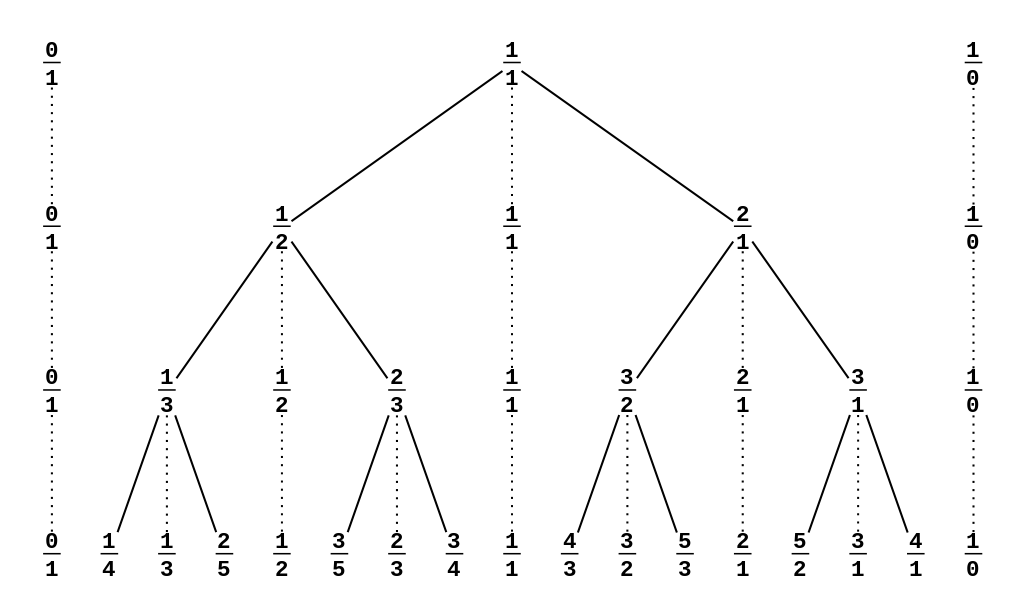
\includegraphics[scale=0.45]{images/stern-brocot1.png} % 插入图片
\end{center}

第$i$层的序列是深度为$i - 1$的Stern-Brocot 树的中序遍历。\par

\textbf{性质:}

\begin{itemize}
\item 单调性\par
在每一层的序列中,真分数是单调递增的。\par
在满足$\displaystyle \frac{a}{b} \leq \frac{c}{d}$,即要证明$\displaystyle \frac{a}{b} \leq \frac{a + c}{b + d} \leq \frac{c}{d}$。\par

此处只证一边,有$\displaystyle \frac{a}{b} \leq \frac{c}{d} \to ad \leq bc \to ad + ab \leq bc + ab \to \frac{a}{b} \leq \frac{a + c}{b + d}$。\par


\item 最简性\par
序列中的分数(除了$\frac{0}{1}, \frac{1}{0}$), 都是最简分数。\par


\end{itemize}


\subsubsection{Farey 序列}

第$i$个Farey序列记作$F_i$, 表示把分母小于等于$i$的所有最简真分数按大小顺序形成的排列。\par

Farey序列$F_i$是Stern-Brocot第$i - 1$次迭代后的序列的子序列。\par

Farey序列同样满足最简性与单调性,对于序列中连续的三个数$\displaystyle \frac{a}{b}, \frac{x}{y}, \frac{c}{d}$,有$x = a + c, y = b + d$。\par
$F_i$的长度$\displaystyle L_i = 1 + \sum\limits_{k = 1}^i \varphi(k)$。\par


\subsubsection{SPOJ-DIVCNT1}

题意:\par

计算$\displaystyle S(n) = \sum \limits_{i=1}^n d(i)$,其中$d(i)$表示$i$的正因子个数。\par

时间复杂度$O(n^{\frac{1}{3}} \log n)$

\begin{lstlisting}
#include<bits/stdc++.h>
typedef long long ll;
typedef __int128 u128;
using namespace std;
const int N = 1e7 + 5;

namespace DIVCNT {
	struct point{
		ll x, y;
		point(ll _x = 0,ll _y = 0){ x = _x; y = _y; }
		point operator + (const point &t) const {
			return point(x + t.x, y + t.y);
		}
	}st[N], L, R, M;
	ll n;
	inline bool inR(ll x,ll y) { return x * y <= n; }
	inline double slope(ll x) { return (double)n / x / x;}
	inline u128 gao(ll _n){
		n = _n;
		u128 ret = 0;
		int t = 0, rt = cbrt(n);
		st[++t] = point(1, 0);
		st[++t] = point(1, 1);
		ll m = sqrt(n), x = n / m, y = m + 1;
		while (1) {
			for (L = st[t--]; !inR(x + L.x, y - L.y); x += L.x, y -= L.y)
				ret += x * L.y + (L.y + 1) * (L.x - 1) / 2;
			if (y <= rt) break;
			for (R = st[t]; inR(x + R.x, y - R.y); R = st[--t]) L = R;
			while (1){
				M = L + R;
				if (!inR(x + M.x, y - M.y)) st[++t] = (R = M);
				else {
					if (slope(x + M.x) <= (double)R.y / R.x) break;
					L = M;
				}
			}
		}
		for (int i = 1; i < y; i++) ret += n / i;
		return ret * 2 - 1ll * m * m;
	}
};

inline void write(u128 x){
	if (x >= 10) write(x / 10);
	putchar(x % 10 + '0');
}

inline void writeln(const u128 &x){
	write(x);
	putchar('\n');
}

int main(){
	int _T; scanf("%d", &_T);
	while (_T--) {
		ll n;
		scanf("%lld", &n);
		writeln(DIVCNT::gao(n));
	}
	return 0;
}
\end{lstlisting}


\subsection{各种表}

\subsubsection{因子个数表}

\begin{itemize}
\item $10^{5}$内, 拥有最大因子个数的数是$83160$, 有$128$个因子
\item $10^{6}$内, 拥有最大因子个数的数是$720720$, 有$240$个因子
\item $10^{7}$内, 拥有最大因子个数的数是$8648640$, 有$448$个因子
\item $10^{8}$内, 拥有最大因子个数的数是$73513440$, 有$768$个因子
\item $10^{9}$内, 拥有最大因子个数的数是$735134400$, 有$1344$个因子
\item $10^{10}$内, 拥有最大因子个数的数是$6983776800$, 有$2304$个因子
\item $10^{11}$内, 拥有最大因子个数的数是$97772875200$, 有$4032$个因子
\item $10^{12}$内, 拥有最大因子个数的数是$963761198400$, 有$6720$个因子
\item $10^{13}$内, 拥有最大因子个数的数是$9316358251200$, 有$10752$个因子
\item $10^{14}$内, 拥有最大因子个数的数是$97821761637600$, 有$17280$个因子
\item $10^{15}$内, 拥有最大因子个数的数是$866421317361600$, 有$26880$个因子
\item $10^{16}$内, 拥有最大因子个数的数是$8086598962041600$, 有$41472$个因子
\item $10^{17}$内, 拥有最大因子个数的数是$74801040398884800$, 有$64512$个因子
\end{itemize}

\section{图论}

\subsection{Dijkstra}


\subsubsection{无向图最小环}

CF 1325E\par
枚举每个起点, 跑$Dijkstra$,对于其中没有状态转移的边,$<u, v>$, 此时$dis[u] + dis[v] + 1$是一个环\par

时间复杂度$O(n^2 \log E)$

\begin{lstlisting}
int pre[N], dis[N], vis[N];
void bfs(int u) {
	queue <int> que;
	for (int i = 1; i < N; ++i) {
		dis[i] = INF;
		vis[i] = 0;
		pre[i] = 0;
	}
	pre[u] = u;
	dis[u] = 0;
	que.push(u);
	while (!que.empty()) {
		int u = que.front(); que.pop();
		for (auto &v : G[u]) {
			if (!vis[v] && dis[v] > dis[u] + 1) {
				vis[v] = 1;
				dis[v] = dis[u] + 1;
				pre[v] = u;
				que.push(v);
			} else {
				if (pre[v] != u && pre[u] != v && dis[v] + dis[u] >= 2) 
					chmin(res, dis[v] + dis[u] + 1); 
			} 
		}
	}
}
\end{lstlisting}

\subsection{Johnson 全源最短路}

添加一个$0$号点,向其它每个点连一条边权为$0$的边。\par
用$SPFA$以$0$号点为源点跑最短路,记为$h_i$, 加入存在一条从$u$到$v$的边, 边权为$w$的边, 则将该边的边权重新设置为$w + h_u - h_v$\par

再以每个点为起点,跑$n$轮$Dijkstra$即可,算法复杂度$O(nm \log n)$\par

\textbf{正确性证明:}\par

重新标注的图上,一条从$s$到$t$的路径$s \rightarrow p_1 \rightarrow p_2 \rightarrow \cdots \rightarrow p_k \rightarrow t$的长度为:

\begin{eqnarray*}
(w(s, p_1) + h_s - h_{p_1}) + (w(p_1, p_2) + h_{p_1} - h_{p_2}) + \cdots + (w(p_k, t) + h_{p_k} - h_t)
\end{eqnarray*}

化简后为:

\begin{eqnarray*}
w(s, p_1) + w(p_1, p_2) + \cdots + w(p_k, t) + h_s - h_t
\end{eqnarray*}

所以对于$s \rightarrow t$的所有路径中,$h_s - h_t$的值不变,可以类比物理中的势能。\par

所以新图上的最短路等价于原图的最短路。\par

根据三角形不等式,新图上任意一条边满足$\displaystyle h_v \leq h_u + w(u, v)$,重新标记后为$\displaystyle w'(u, v) = w(u, v) + h_u - h_v \geq 0$,满足非负。\par


洛谷P5905\par

题意:给出$n$个点$m$条边的带权有向图, 求所有点对的最短路径长度, 边权可能非负,图中可能有重边和自环。\par

若图中有负环,输出$-1$\par

$1 \leq n \leq 3 \cdot 10^3, 1 \leq m \leq 6 \cdot 10^3$\par



\begin{lstlisting}
#include <bits/stdc++.h>
using namespace std;
typedef long long ll;
const int N = 6e3 + 10, INF = 1e9;
int n, m;

struct Graph {
	struct E { int to, nx; ll w; }e[N << 1]; int h[N], cnt;
	void init(int n) { for (int i = 0; i <= n; ++i) h[i] = -1; cnt = -1; }
	void addedge(int u, int v, ll w = 0) { e[++cnt] = { v, h[u], w}; h[u] = cnt; } 
}G;

struct SPFA {
	ll dis[N]; int cnt[N]; bool used[N];
	// true 没有负环
	// false 有负环
	bool gao(int s) {
		for (int i = 0; i <= n; ++i) {
			dis[i] = INF;
			cnt[i] = 0;
			used[i] = 0;
		}
		queue <int> que;
		dis[s] = 0; used[s] = 1;
		que.push(s);
		while (!que.empty()) {
			int u = que.front(); que.pop();
			used[u] = 0;
			for (int i = G.h[u]; ~i; i = G.e[i].nx) {
				int v = G.e[i].to; ll w = G.e[i].w;
				if (dis[v] > dis[u] + w) {
					dis[v] = dis[u] + w;
					if (!used[v]) {
						used[v] = 1;
						que.push(v);
						++cnt[v]; 
						if (cnt[v] == n) return false;
					}
				}
			}
		}
		return true;
	}
}spfa;

struct Dijkstra {
	struct node {
		int u; ll w;
		node(int u = 0, ll w = 0) : u(u), w(w) {}
		bool operator < (const node &other) const { return w > other.w; }		
	};
	ll dis[N]; bool used[N]; 
	void gao(int s) {
		for (int i = 0; i <= n; ++i) {
			dis[i] = INF;
			used[i] = 0;
		}
		priority_queue <node> pq;
		dis[s] = 0;
		pq.push(node(s, dis[s]));
		while (!pq.empty()) {
			int u = pq.top().u; pq.pop();
			if (used[u]) continue;
			used[u] = 1;
			for (int i = G.h[u]; ~i; i = G.e[i].nx) {
				int v = G.e[i].to; ll w = G.e[i].w;
				if (!used[v] && dis[v] > dis[u] + w) {
					dis[v] = dis[u] + w;
					pq.push(node(v, dis[v]));
				}
			}
		}
	}
}dij;

int main() {
	scanf("%d%d", &n, &m);
	G.init(n);
	for (int i = 1, u, v, w; i <= m; ++i) {
		scanf("%d%d%d", &u, &v, &w);
		G.addedge(u, v, w);
	}
	for (int i = 1; i <= n; ++i)
		G.addedge(0, i, 0);
	if (!spfa.gao(0)) {
		puts("-1");
		return 0;	
	}
	ll *h = spfa.dis;
	for (int u = 1; u <= n; ++u) {
		for (int i = G.h[u]; ~i; i = G.e[i].nx) {
			int v = G.e[i].to;
			G.e[i].w += h[u] - h[v];
		}
	}
	for (int i = 1; i <= n; ++i) {
		dij.gao(i);
		ll *f = dij.dis;
		ll res = 0;
		for (int j = 1; j <= n; ++j) {
			if (f[j] == INF) res += 1ll * j * INF;
			else res += 1ll * j * (f[j] + h[j] - h[i]);
		}
		printf("%lld\n", res);
	}
	return 0;
}
\end{lstlisting}

\subsection{最小生成树}

\subsubsection{CDQ分治动态维护}

BZOJ 2001\par
题意:\par
$n$个城市, $m$条边,$q$次修改边权操作,修改不独立,每次修改后给出当前图最小生成树权值和。\par

思路:\par

\begin{itemize}
\item Reduction:\par
把修改$L-R$所影响到的所有边的边权设为$\infty$,然后跑MST,则此时不在修改边集并且不在最小生成树的边集里的边直接舍去, 因为不管怎样这些边都不会被选中。

\item Contraction: \par
把修改$L-R$所影响到的所有边的边权设为$-\infty$,然后跑MST,则此时不在修改边集并且在最小生成树的边集里的边直接选中, 因为不管怎样这些边都会被选中,在下一层分治操作中就不用管这些边了,我们假设所有锁定边为$must$,往下传就好了。
\end{itemize}

考虑每一层的边数与当前图的点数同阶,每次缩边缩掉的是$-\infty$生成树中的未修改边,相当于割掉了$-\infty$生成树中的修改边, 显然最多割掉$O(len)$条边,
$len$为当前层修改边条树, 那么最多分裂成$O(len)$个联通块, 每层图的点数就是$O(len)$级别的。\par

其实不用回滚并茶集,每次直接将当前边集涉及到的点清空以下即可,因为清空复杂度和当前边数同阶。\par
总的复杂度为$O(n \log^2 n)$

\begin{lstlisting}
#include <bits/stdc++.h>
#define SZ(x) (int(x.size()))
using namespace std;
typedef long long ll;
const int N = 5e4 + 10;
const int INF = 0x3f3f3f3f;
int n, m, q, eW[N];

struct Edge { 
	int u, v, id; ll w;
	bool operator < (const Edge &other) const { return w < other.w; }
}e[N];

struct qNode { int id; ll val, ans; } qrr[N]; 

struct UFS {
	int fa[N];
	int find(int x) { return fa[x] == 0 ? x : fa[x] = find(fa[x]); }
	bool merge(int u, int v) {
		int fu = find(u), fv = find(v);
		if (fu != fv) {
			fa[fu] = fv;
			return true;
		}
		return false;
	}
	void reset(const vector <Edge> &e) { for (int i = 0; i < SZ(e); ++i) fa[e[i].u] = fa[e[i].v] = 0; }
}ufs;

namespace CDQ {
	int tag[N];
	vector <Edge> t[30], tmp, ttmp; 
	//删除无用边
	void Reduction() {
		ufs.reset(tmp);
		sort(tmp.begin(), tmp.end());
		int cur = 0;
		for (int i = 0, u, v; i < SZ(tmp); ++i) {
			u = tmp[i].u, v = tmp[i].v;
			if (tmp[i].w == INF || ufs.merge(u, v)) {
				tmp[cur] = tmp[i];
				tag[tmp[cur].id] = cur;
				cur++;
			}
		}
		tmp.resize(cur);
	}
	//缩掉必须边
	void Contraction(ll &must) {
		ufs.reset(tmp);
		sort(tmp.begin(), tmp.end());
		ttmp.clear(); 
		for (int i = 0, u, v; i < SZ(tmp); ++i) {
			u = tmp[i].u, v = tmp[i].v;
			if (ufs.merge(u, v)) {
				ttmp.push_back(tmp[i]);
			}
		}
		ufs.reset(ttmp);
		for (int i = 0, u, v; i < SZ(ttmp); ++i) {
			u = ttmp[i].u, v = ttmp[i].v;
			if (ttmp[i].w != -INF && ufs.merge(u, v)) {
				must += ttmp[i].w;
			}
		}
		int cur = 0;
		for (int i = 0; i < SZ(tmp); ++i) {
			int u = ufs.find(tmp[i].u), v = ufs.find(tmp[i].v);
			if (u != v) {
				tmp[cur] = tmp[i];
				tag[tmp[cur].id] = cur;
				tmp[cur].u = u;
				tmp[cur].v = v;
				++cur;
			}
		}
		tmp.resize(cur);
	}
	void solve(int l, int r, int dep, ll must) { 
		if (l == r) eW[qrr[l].id] = qrr[l].val;
		for (int i = 0; i < SZ(t[dep]); ++i) {
			t[dep][i].w = eW[t[dep][i].id];
			tag[t[dep][i].id] = i;
		}
		tmp = t[dep];
		if (l == r) {
			qrr[l].ans = must;
			ufs.reset(tmp);
			sort(tmp.begin(), tmp.end());
			for (int i = 0, u, v; i < SZ(tmp); ++i) {
				u = tmp[i].u, v = tmp[i].v;
				if (ufs.merge(u, v)) {
					qrr[l].ans += tmp[i].w;
				} 
			}
			return;
		}
		for (int i = l; i <= r; ++i) tmp[tag[qrr[i].id]].w = INF; 
		Reduction();
		for (int i = l; i <= r; ++i) tmp[tag[qrr[i].id]].w = -INF;
		Contraction(must);
		t[dep + 1] = tmp;
		int mid = (l + r) >> 1;
		solve(l, mid, dep + 1, must);
		solve(mid + 1, r, dep + 1, must);
	}
	void gao() {
		memset(tag, 0, sizeof tag);
		t[0].clear();
		for (int i = 1; i <= m; ++i) 
			t[0].push_back(e[i]);
		solve(1, q, 0, 0);
	}
}

int main() {
	scanf("%d%d%d", &n, &m, &q);
	for (int i = 1; i <= m; ++i) {
		e[i].id = i;
		scanf("%d%d%lld", &e[i].u, &e[i].v, &e[i].w);
		eW[i] = e[i].w;
	}
	for (int i = 1; i <= q; ++i) {
		scanf("%d%lld", &qrr[i].id, &qrr[i].val);
	}
	CDQ::gao();
	for (int i = 1; i <= q; ++i) printf("%lld\n", qrr[i].ans);
	return 0;
}
\end{lstlisting}

\subsection{二分图最大权匹配(KM)}
UOJ80\par
$KM$本质是求最佳匹配的(即先保证匹配边最多,再保证权值最大),但是可以通过添加权值为$0$的边使得肯定存在完备匹配,那么就是求最大权匹配了。\par
几个概念:\par
\begin{itemize}
\item 顶标:给每个顶点赋一个数值,成为该顶点的定标。
\item 可行顶标:如果对于所有的边,满足此边两端的两个顶点的定标和不小于此边权重,则称这一组顶标为可行顶标。
\item 相等子图:在当前顶标下,满足边两端的两个顶点的定标和正好等于此边权重的所有边,所构成的子图。
\end{itemize}
相等子图的性质:\par
\begin{itemize}
\item 在任意时刻,相等子图上的最大权匹配一定小于等于相等子图的顶标和。
\item 在任意时刻,相等子图的顶标和即为所有顶点的顶标和。
\item 扩充相等子图后,相等子图的顶标和将会减小。
\item 当相等子图的最大匹配为原图的完备匹配时,匹配边的权值和等于所有顶点的顶标和,此匹配即为最佳匹配
\end{itemize} \par
$KM$算法过程中任意时刻都满足$x_i + y_j \leq w_{i, j}$,所以最终可以求得$\sum x_i + \sum y_j$的最小值,但是相等子图上的最大权匹配一定小于等于相等子图的顶标和,所以取等号时,边权和最大,顶标和最小。\par
相反,如果要满足$x_i + y_j \leq w_{i, j}$,并且使得$\sum x_i + \sum y_j$最大,只需要取负号满足$-(x_i + y_j) \leq -w_{i, j}$,最后将结果也取负即可。\par


\begin{lstlisting}
#include <bits/stdc++.h>
using namespace std;
using ll = long long;
//时间复杂度O(nx * nx * ny) 
//点的编号从1开始
struct KM {
	static const int N = 4e2 + 10;
	static const int INF = 0x3f3f3f3f;
	int lx[N], ly[N], slack[N], w[N][N]; //以上为权值类型
	int vx[N], vy[N], pre[N], left[N], right[N], nl, nr, n;
	void match(int& u) {
		for (; u; swap(u, right[pre[u]])) 
			left[u] = pre[u];
	}
	void bfs(int u) {
		static int q[N], front, rear;
		front = 0; vx[q[rear = 1] = u] = true;
		while (true) {
			while (front < rear) {
				int u = q[++front];
				for (int v = 1; v <= n; ++v) {
					int tmp; 
					if (vy[v] || (tmp = lx[u] + ly[v] - w[u][v]) > slack[v])
						continue;
					pre[v] = u;
					if (!tmp) {
						if (!left[v]) return match(v);
						vy[v] = vx[q[++rear] = left[v]] = true;
					} else {
						slack[v] = tmp;
					}
				}
			}
			int a = INF;
			for (int i = 1; i <= n; ++i) {
				if (!vy[i] && a > slack[i]) a = slack[u = i];
			}
			for (int i = 1; i <= n; ++i) {
				if (vx[i]) lx[i] -= a;
				if (vy[i]) ly[i] += a;
				else slack[i] -= a;
			}
			if (!left[u]) return match(u);
			vy[u] = vx[q[++rear] = left[u]] = true;
		}
	}
	void exec() {
		for (int i = 1; i <= n; ++i) {
			for (int j = 1; j <= n; ++j) {
				slack[j] = INF;
				vx[j] = vy[j] = false;
			}
			bfs(i);
		}
	}
	void init(int _nl, int _nr) {
		nl = _nl, nr = _nr;
		n = max(nl, nr);
		for (int u = 1; u <= n; ++u) {
			lx[u] = ly[u] = 0;
			left[u] = right[u] = 0;
			for (int v = 1; v <= n; ++v) {
				w[u][v] = 0;
			}
		}
	}
	ll work() {
		for (int u = 1; u <= n; ++u) {
			for (int v = 1; v <= n; ++v) {
				lx[u] = max(lx[u], w[u][v]);
			}
		}
		exec();
		ll ans = 0;
		for (int i = 1; i <= n; ++i) {
			ans += lx[i] + ly[i];
		}
		return ans;
	}
	void output() {
		for (int i = 1; i <= nl; ++i) {
			printf("%d%c", (w[i][right[i]] ? right[i] : 0), " \n"[i == nl]);
		}
	}
}km;
int nl, nr, m;

int main() {
	while (scanf("%d%d%d", &nl, &nr, &m) != EOF) {
		km.init(nl, nr);
		for (int i = 1, u, v, w; i <= m; ++i) {
			scanf("%d%d%d", &u, &v, &w);
			km.w[u][v] = w;
		}
		printf("%lld\n", km.work()); 
		km.output();
	}
	return 0;
}
\end{lstlisting}

\section{离散化}
\begin{lstlisting}
struct Hash {
	vector <int> a;
	int& operator[](int x) { return a[x - 1]; }
	int size() { return a.size(); }
	void init() { a.clear(); }
	void add(int x) { a.push_back(x); }
	void gao() { sort(a.begin(), a.end()); a.erase(unique(a.begin(), a.end()), a.end()); }
	int get(int x) { return lower_bound(a.begin(), a.end(), x) - a.begin() + 1; }	
}hs;
\end{lstlisting}

\section{PB-DS}
\begin{lstlisting}
#include<ext/pb_ds/assoc_container.hpp>
#include<ext/pb_ds/tree_policy.hpp>//用tree
#include<ext/pb_ds/hash_policy.hpp>//用hash
#include<ext/pb_ds/trie_policy.hpp>//用trie
#include<ext/pb_ds/priority_queue.hpp>//用priority_queue
using namespace __gnu_pbds;
//或者:
#include<bits/extc++.h>
using namespace __gnu_pbds;
//bits/extc++.h与bits/stdc++.h类似,bits/extc++.h是所有拓展库,bits/stdc++.h是所有标准库
\end{lstlisting}

\subsection{Hash-Table}
\begin{lstlisting}
#include <bits/stdc++.h>
#include <bits/extc++.h>
using namespace std;
using namespace __gnu_pbds;
const int N = 1e5 + 10;
//拉链法
//cc_hash_table<string, int> h;

//探测法
gp_hash_table<string, int> h;
int n;
char s[N];

int main() {
	while (scanf("%d", &n) != EOF) {
		for (int i = 1; i <= n; ++i) {
			scanf("%s", s + 1);
			//支持find和[]
			if (h.find(s + 1) == h.end()) {
				h[s + 1] = 1;
			}
		}
		printf("%d\n", (int)h.size());
	}
	return 0;
}
\end{lstlisting}

\subsection{Hash-Map}

\begin{lstlisting}
#include<bits/stdc++.h>
#include<bits/extc++.h>
#define fi first
#define se second
using namespace std;

struct splitmix64_hash {
    static uint64_t splitmix64(uint64_t x) {
        x += 0x9e3779b97f4a7c15;
        x = (x ^ (x >> 30)) * 0xbf58476d1ce4e5b9;
        x = (x ^ (x >> 27)) * 0x94d049bb133111eb;
        return x ^ (x >> 31);
    }
    size_t operator()(uint64_t x) const {
        static const uint64_t FIXED_RANDOM = std::chrono::steady_clock::now().time_since_epoch().count();
        return splitmix64(x + FIXED_RANDOM);
    }
};

template <typename K, typename V, typename Hash = splitmix64_hash>
using hash_map = __gnu_pbds::gp_hash_table<K, V, Hash>;

template <typename K, typename Hash = splitmix64_hash>
using hash_set = hash_map<K, __gnu_pbds::null_type, Hash>;

int main() {
	hash_map<int64_t, int> mp;
	int n = 1e7;
	for (int i = 1; i <= n; ++i) {
		mp[i] = 1;
	}
	long long res = 0;
	for (auto &it : mp)
		res += it.fi;
	cout << res << endl;
	return 0;
}
\end{lstlisting}

\subsection{Priority-Queue}
一切的开始: 
\begin{lstlisting}
#include <ext/pb_ds/assoc_container.hpp>
#include <ext/pb_ds/priority_queue.hpp>
using namespace __gnu_pbds;
\end{lstlisting}

\subsubsection{TAG类型}
priority\underline{~~}queue<int,greater<int>,TAG> Q;//小根堆,大根堆写less<int> \par
其中的TAG为类型,有以下几种:\par
\begin{itemize}
\item pairing\underline{~~}heap\underline{~~}tag push和join 为$O(1)$,其余为均摊$\Theta(log n)$\par
\item thin\underline{~~}heap\underline{~~}tag 只支持push和pop,均为均摊$\Theta(logn)$\par
\item binomial\underline{~~}heap\underline{~~}tag push为均摊$O(1)$,其余为$\Theta(log n)$\par
\item rc\underline{~~}binomial\underline{~~}heap\underline{~~}tag push为$O(1)$,其余为$\Theta(log n)$\par
\item binary\underline{~~}heap\underline{~~}tag push为$O(1)$, 不支持join, 其余为$\Theta(log n)$, 但是如果只有increase\underline{~~}key,那么modify为均摊$O(1)$\par
\item 其中pairing\underline{~~}heap\underline{~~}tag最快,并且默认就为pairing\underline{~~}heap\underline{~~}tag\par
\end{itemize}

选择:
\begin{itemize}
\item 在只有push, pop的时候, binary\underline{~~}heap\underline{~~}tag速度比较快,在绝大多数情况下优于std::priority\underline{~~}queue
\item 在有modify操作的时候,可以考虑采用pairing\underline{~~}heap\underline{~~}tag, thin\underline{~~}heap\underline{~~}tag或手写数据结构
\item 只有push, pop, join的时候,可以考虑用pairing\underline{~~}heap\underline{~~}tag或binomial\underline{~~}heap\underline{~~}tag
\end{itemize}

\subsubsection{基本操作}
\begin{itemize}
\item it = Q.push(x);  插入时会返回迭代器
\item Q.clear(); 
\item Q.pop(); 
\item Q.top();
\item Q.join(b); // b元素加入到Q中,b清空
\item Q.empty();
\item Q.size(); 
\item Q.modify(it,6);
\item Q.erase(it);
\item 迭代器是point\underline{~~}iterator,可以用迭代器遍历整个优先队列
\end{itemize}

\subsubsection{BZOJ 3040}
堆优化Dijkstra
\begin{lstlisting}
#include <bits/stdc++.h>
#include <bits/extc++.h>
using namespace std;
using namespace __gnu_pbds;

#define ll long long
#define INFLL 0x3f3f3f3f3f3f3f3f
#define N 1000010
#define M 10000010
int n, m, T, rxa, rxc, rya, ryc, rp;
struct Graph {
	struct node {
		int to, nx, w;
		node() {}
		node (int to, int nx, int w) : to(to), nx(nx), w(w) {}
	}a[M];
	int head[N], pos;
	void init() {
		memset(head, -1, sizeof head);
		pos = 0;
	}
	inline void add(int u, int v, int w) {
		a[pos] = node(v, head[u], w); head[u] = pos++; 
	}
}G;
#define erp(u) for (int it = G.head[u], v = G.a[it].to, w = G.a[it].w; ~it; it = G.a[it].nx, v = G.a[it].to, w = G.a[it].w)

struct node {
	int u; ll w;
	node() {}
	node (int u, ll w) : u(u), w(w) {}
	bool operator < (const node &other) const {
		return w > other.w;
	}
};
//less是大根堆,表示使用!<来当排序规则,priority_queue 默认用的也是less
#define heap __gnu_pbds::priority_queue <node, less<node>, pairing_heap_tag>

ll dis[N]; 
heap::point_iterator id[N];
heap pq;
void Dijkstra() {
	for (int i = 2; i <= n; ++i) {
		dis[i] = INFLL;
		id[i] = 0;
	}
	while (!pq.empty()) pq.pop();
	dis[1] = 0;
	id[1] = pq.push(node(1, 0)); 
	while (!pq.empty()) {
		int u = pq.top().u; pq.pop();
		erp(u) if (dis[v] > dis[u] + w) {
			dis[v] = dis[u] + w;
			if (id[v] == 0) {
				id[v] = pq.push(node(v, dis[v]));
			} else {
				pq.modify(id[v], node(v, dis[v]));
			}
		}
	}
}

int main() {
	while (scanf("%d%d", &n, &m) != EOF) {
		scanf("%d%d%d%d%d%d", &T, &rxa, &rxc, &rya, &ryc, &rp);
		G.init();
		ll x = 0, y = 0, a, b;
		for (int i = 1; i <= T; ++i) {
			x = (x * rxa + rxc) % rp;
			y = (y * rya + ryc) % rp;
			a = min(x % n + 1, y % n + 1);
			b = max(x % n + 1, y % n + 1);
			G.add(a, b, 100000000 - 100 * a);
		}
		for (int i = 1, u, v, w; i <= m - T; ++i) {
			scanf("%d%d%d", &u, &v, &w);
			G.add(u, v, w);
		}
		Dijkstra();
		printf("%lld\n", dis[n]);
	}
	return 0;
}
\end{lstlisting}

\subsection{Tree}

TAG有rb\_tree, splay\_tree, ov\_tree, 后两种较慢,一般使用rb\_tree\par

\subsubsection{基本操作}
\begin{lstlisting}=
#include<ext/pb_ds/assoc_container.hpp>
#include<ext/pb_ds/tree_policy.hpp>
using namespace __gnu_pbds;
#define pII pair<int,int>
#define mp(x,y) make_pair(x,y) 
tree<pII,null_type,less<pII>,rb_tree_tag,tree_order_statistics_node_update> tr;
pII //存储的类型
null_type //无映射(低版本g++为null_mapped_type)
如果是map,这里是Mapped,即map中的第二关键字
less<pII> //从小到大排序
rb_tree_tag //红黑树
tree_order_statistics_node_update //更新方式 
tr.insert(mp(x,y)); //插入;
tr.erase(mp(x,y)); //删除;
tr.order_of_key(pII(x,y)); //求排名 
tr.find_by_order(x); //找第x + 1小的元素的迭代器,如果x太大会返回end()
tr.join(b); //将b并入tr,前提是两棵树类型一样且没有重复元素 
tr.split(v,b); //分裂,key小于等于v的元素属于tr,其余的属于b
tr.lower_bound(x); //返回第一个大于等于x的元素的迭代器
tr.upper_bound(x); //返回第一个大于x的元素的迭代器
//以上所有操作的时间复杂度均为O(logn) 
\end{lstlisting}

\subsubsection{Luogu P3369}
题意:\par
维护一些操作:
\begin{enumerate}
\item 插入x数
\item 删除x数(若有多个相同的数,应只删除一个)
\item 查询x数的排名(若有多个相同的数,应输出最小的排名)
\item 查询排名为x的数
\item 求x的前驱(前驱定义为小于x,且最大的数)
\item 求x的后继(后继定义为大于x,且最小的数)
\end{enumerate}
\begin{lstlisting}
#include <bits/stdc++.h>
#include<ext/pb_ds/assoc_container.hpp>
#include<ext/pb_ds/tree_policy.hpp>
using namespace std;
using namespace __gnu_pbds;
using pII = pair<int, int>;
#define fi first
#define se second
tree<pII,null_type,less<pII>,rb_tree_tag,tree_order_statistics_node_update> rbtree;

int main() {
	int n; scanf("%d", &n);
	rbtree.clear();
	int op, x;
	for (int i = 1; i <= n; ++i) {
		scanf("%d%d", &op, &x);
		if (op == 1) {
			rbtree.insert(pII(x, i));	
		} else if (op == 2) {
			rbtree.erase(rbtree.lower_bound(pII(x, 0)));
		} else if (op == 3) {
			printf("%d\n", (int)rbtree.order_of_key(pII(x, 0)) + 1);
		} else if (op == 4) {
			int ans = rbtree.find_by_order(x - 1)->fi;
			printf("%d\n", ans);
		} else if (op == 5) {
			int ans = (--rbtree.lower_bound(pII(x, 0)))->fi;
			printf("%d\n", ans);
		} else if (op == 6) {
			int ans = rbtree.upper_bound(pII(x, n))->fi;
			printf("%d\n", ans);
		}
	}
	return 0;
}
\end{lstlisting}

\subsubsection{CF 459D}
以pari<int, int>作为键值,int作为权值能够查询区间权值和的map。\par
只能插入删除,不可使用[]操作符。\par

\begin{lstlisting}
#include <bits/stdc++.h>
#include <bits/extc++.h>
#define fi first
#define se second
using namespace __gnu_pbds;
using namespace std;
using pII = pair <int, int>;
using ll = long long;
constexpr int N = 1e6 + 10;
int n, m, a[N], f[N];
unordered_map <int, int> cnt;

template<class Node_CItr, class Node_Itr, class Cmp_Fn, class _Alloc>
struct map_node_update {
    virtual Node_CItr node_begin() const = 0;
    virtual Node_CItr node_end() const = 0;
    typedef int metadata_type;
	const static int INF = 0x3f3f3f3f;
    void operator() (Node_Itr it, Node_CItr end_it) {
        Node_Itr l = it.get_l_child();
        Node_Itr r = it.get_r_child();
        metadata_type left = 0, right = 0;
        if(l != end_it) left = l.get_metadata();
        if(r != end_it) right = r.get_metadata();
        const_cast<metadata_type &>(it.get_metadata()) = 
			left + right + (*it)->second; 
    }
	metadata_type querysum(pII x) {
		metadata_type ans = 0;
        Node_CItr it = node_begin();
		while (it != node_end()) {
			Node_CItr l = it.get_l_child();
			Node_CItr r = it.get_r_child();
			//x比当前节点要小,走向左儿子
            if(Cmp_Fn()(x, (*it)->first)) {
                it = l;
    		} else {
				//x大于等于当前节点
				ans += (*it)->second;
                if(l != node_end()) ans += l.get_metadata();
                it = r;
            }
		}
		return ans;
	}
	//[l, r]范围内的权值
	metadata_type querysum(int l, int r) { 
		if (l > r) return 0;
		return querysum(pII(r, INF)) - querysum(pII(l, -INF)); 
	}
};
//pII fi key se id Mapeed value
//不可使用非标准的[]操作, 为了防止重复,用pair当键值, se是id
tree<pII, int, less<pII>, rb_tree_tag, map_node_update> rbtree; 

int main() {
	scanf("%d", &n);
	cnt.clear();
	for (int i = 1; i <= n; ++i) scanf("%d", a + i);
	for (int i = 1; i <= n; ++i) {
		++cnt[a[i]];
		f[i] = cnt[a[i]];
	}
	cnt.clear();
	rbtree.clear();
	ll res = 0;
	for (int i = n; i >= 1; --i) {
		++cnt[a[i]];
		res += rbtree.querysum(1, f[i] - 1);
		rbtree.insert(make_pair(pII(cnt[a[i]], i), 1)); 
	}
	printf("%lld\n", res);
	return 0;
}
\end{lstlisting}

\subsection{Trie}

\subsubsection{基本操作}
\begin{lstlisting}
typedef trie<string,null_type,trie_string_access_traits<>,pat_trie_tag,trie_prefix_search_node_update> tr;
//第一个参数必须为字符串类型,tag也有别的tag,但pat最快,与tree相同,node_update支持自定义
tr.insert(s); //插入s 
tr.erase(s); //删除s 
tr.join(b); //将b并入tr 
//pair的使用如下:
pair<tr::iterator,tr::iterator> range=tr.prefix_range(s);
for(tr::iterator it = range.first; it != range.second; it++)
    cout << *i t<< ' ' <<endl;
//pair中第一个是起始迭代器,第二个是终止迭代器,遍历过去就可以找到所有字符串了。 
\end{lstlisting}

\subsubsection{Times1414}
\begin{lstlisting}
#include<bits/stdc++.h>
#include<ext/pb_ds/assoc_container.hpp>
#include<ext/pb_ds/trie_policy.hpp>
using namespace std;
using namespace __gnu_pbds; 
trie<string,null_type,trie_string_access_traits<>,pat_trie_tag,trie_prefix_search_node_update> tr;

int main() {
	ios::sync_with_stdio(false);
	cin.tie(nullptr); cout.tie(nullptr);
	tr.clear(); tr.insert("sun");
	string s;
	while (cin >> s) {
		if (s[0] == '?') {
			s = s.substr(1);
			cout << s << "\n";
			auto range = tr.prefix_range(s);
			int t = 0;
			for (auto it = range.first; t < 20 && it != range.second; ++t, ++it) {
				cout << "  " << *it << "\n";
			}
		} else {
			tr.insert(s.substr(1));
		}
	}
	return 0;
};
\end{lstlisting}


\subsection{rope}
一切的开始:
\begin{lstlisting}
#include <ext/rope>
using namespace __gnu_cxx;
\end{lstlisting}

\subsubsection{基本操作}
\begin{itemize}
\item insert(int pos, T *s, int n)\par
将字符串$s$的前$n$位插入$rope$的下标$pos$处, 如没有参数$n$则将字符串$s$的所有位都插入$rope$的下标$pos$处
\item append(T *s,int pos,int n) \par
把字符串$s$中从下标$pos$开始的$n$个字符连接到$rope$的结尾, 如没有参数$n$则把字符串$s$中下标$pos$后的所有字符连接到$rope$的结尾, 如没有参数$pos$则把整个字符串$s$连接到$rope$的结尾
\item substr(int pos, int len) \par
提取$rope$的从下标$pos$开始的$len$个字符
\item at(int x) \par
访问$rope$的下标为$x$的元素
\item erase(int pos, int num) \par
从$rope$的下标$pos$开始删除$num$个字符
\item copy(int pos, int len, T *s) \par
从$rope$的下标$pos$开始的$len$个字符用字符串$s$代替,如果$pos$后的位数不够就补足
\item replace(int pos, T *s)\par
从$rope$的下标$pos$开始替换成字符串$s$,$s$的长度为从$pos$开始替换的位数,如果$pos$后的位数不够就补足
\item length()\par
获取rope当前长度
\end{itemize}
原理是用块状链表实现,时间复杂度$O(n\sqrt{n})$


\subsubsection{进阶操作}
\begin{itemize}
\item 区间翻转\par
维护一正一反两个$rope$, 翻转等价于交换两个子串
\item 区间循环位移\par
拆成多个子串,再连接起来
\item 区间字符自增$1$,即$a->b, b->c, \cdots, z->a$\par
维护$26$个$rope$
\item 可持久化\par
维护根结点,可以直接复制之前版本的根结点是$O(1)$的。\par
可以参考BZOJ 3673\par
\end{itemize}


\subsubsection{BZOJ 1269}

题意:\par
\begin{itemize}
\item MOVE(k),将光标移动第$k$个字符后
\item INSERT(n, s), 在光标后插入长度为$n$的字符串$s$,光标位置不变
\item DELETE(n), 删除光标后的$n$个字符
\item ROTATE(n), 反转光标后的$n$个字符
\item GET(), 输出光标后的第一个字符
\item PREV(), 光标前移一个字符
\item NEXT(), 光标后移一个字符
\end{itemize}

\begin{lstlisting}
#include <bits/stdc++.h>
#include <bits/extc++.h>
using namespace std;
using namespace __gnu_cxx;
const int N = 2e6 + 10; 
rope <char> A, B, T;
int n, pos, len;
char s[N], revs[N];

int main() {
	int _T;
	scanf("%d", &_T);
	char op[5];
	pos = 0;
	while (_T--) {
		scanf("%s", op);
		if (op[0] == 'M') {
			scanf("%d", &pos);
		} else if (op[0] == 'I') {
			scanf("%d", &n);
			for (int i = 0; i < n; ++i) {
				do { s[i] = getchar(); }
				while (s[i] == '\n');
				revs[n - i - 1] = s[i];
			}
			s[n] = revs[n] = 0;
			len = A.length();
			A.insert(pos, s);
			B.insert(len - pos, revs);
		} else if (op[0] == 'D') {
			scanf("%d", &n);
			len = A.length();
			A.erase(pos, n);
			B.erase(len - pos - n, n);
		} else if (op[0] == 'R') {
			scanf("%d", &n);
			len = A.length();
			T = A.substr(pos, n);
			A = A.substr(0, pos) + B.substr(len - pos - n, n) + A.substr(pos + n, len - pos - n);
			B = B.substr(0, len - pos - n) + T + B.substr(len - pos, pos); 	
		} else if (op[0] == 'G') {
			printf("%c\n", A.at(pos));
		} else if (op[0] == 'P') {
			--pos;
		} else if (op[0] == 'N') {
			++pos;
		}
	}	
	return 0;
}
\end{lstlisting}

\subsubsection{BZOJ 3673}
\begin{itemize}
\item $1\;a\;b$,合并$a$, $b$所在集合
\item $2\;k$,回到第$k$次操后之后的状态(查询算一次操作)
\item $3\;a\;b$,询问$a$和$b$是否在同一集合
\end{itemize}
\begin{lstlisting}
#include <bits/stdc++.h>
#include <bits/extc++.h>
using namespace std;
using namespace __gnu_cxx;
const int N = 2e5 + 10;
int n, q, a[N];

struct UFS {
	rope <int> *fa;
	int find(int x) {
		if (fa->at(x) == 0) return x;
		fa->replace(x, find(fa->at(x)));
		return fa->at(x);
	}
	void merge(int x, int y) {
		int fx = find(x), fy = find(y);
		if (fx != fy) {
			fa->replace(fx, fy);
		}
	}
	bool same(int x, int y) { return find(x) == find(y); }
}ufs[N]; 

int main() {
    scanf("%d%d", &n, &q);
	memset(a, 0, sizeof (a[0]) * (n + 5));
	//用数组新建rope
	ufs[0].fa = new rope<int> (a, a + 1 + n);
   	for (int i = 1, op, x, y, k; i <= q; ++i) {
		scanf("%d", &op);
		//复制之前版本的rope,不会影响之前的版本
		ufs[i].fa = new rope<int> (*ufs[i - 1].fa);
		if (op == 1) {
			scanf("%d%d", &x, &y);
			ufs[i].merge(x, y);
		} else if (op == 2) {
			scanf("%d", &k);
			//直接继承,会影响之前的版本
			ufs[i].fa = ufs[k].fa; 
		} else if (op == 3) {
			scanf("%d%d", &x, &y);
			printf("%d\n", ufs[i].same(x, y));
		}
	} 
}
\end{lstlisting}


\subsubsection{Luogu P3391}
题意:\par
维护序列的区间翻转\par
\begin{lstlisting}
#include <bits/stdc++.h>
#include <bits/extc++.h>
using namespace std;
using namespace __gnu_cxx;
const int N = 1e5 + 10; 
rope <int> A, B, T; 
int n, q, a[N];

int main() {
	while (scanf("%d%d", &n, &q) != EOF) {
		A.clear(); B.clear();
		for (int i = 1; i <= n; ++i) a[i] = i;
		A = rope<int>(a, a + 1 + n);
		reverse(a + 1, a + 1 + n);
		B = rope<int>(a, a + 1 + n);
		for (int i = 1, l, r; i <= q; ++i) {
			scanf("%d%d", &l, &r);
			T = A.substr(l, r - l + 1);
			A = A.substr(0, (l - 1) + 1) + B.substr(n - r + 1, r - l + 1) + A.substr(r + 1, n - (r + 1) + 1);
			B = B.substr(0, n - r + 1) + T + B.substr(n - l + 2, n - (n - l + 2) + 1); 
		}
		for (int i = 1; i <= n; ++i) 
			printf("%d%c", A[i], " \n"[i == n]);
	}
	return 0;
}
\end{lstlisting}

\section{广义RMQ}

普通的$RMQ$仅仅支持能够重复贡献信息的区间查询功能,如区间最值\par
但是我们可以通过一个黑科技来实现$O(n \log n) + O(1) + O(n \log n)$的复杂度实现支持结合律和快速合并的信息的区间查询\par

这里以区间乘法为例:\par
设$A_{k,i}=\prod\limits_{j=\left\lfloor\frac i{2^k}\right\rfloor2^k}^ia_j,B_{k,i}=\prod\limits_{j=i}^{\left\lceil\frac{i+1}{2^k}\right\rceil2^k-1}a_j$\par

$A_{k,i}$表示的是($\leq i$的最大的$2^k$的倍数)到$i$这一段数的乘积,$B_{k,i}$表示的是$i$到($> i$的最小的$2^k$的倍数$-1$)这一段数的乘积,这两个都可以$O(n\log n)$预处理\par

对于询问$[l,r]$,如果$l=r$那么答案就是$a_l$,下面讨论$l < r$的情况\par

如果我们可以找到一个$k$,使得$[l+1,r]$中只有一个$2^k$的倍数,那么$B_{k,l}A_{k,r}$就是答案\par

容易验证一个满足要求的$k$就是$\log_2\left(\text{highbit}(l \oplus r)\right)$。\par

CodeChef-SEGPROD
\begin{lstlisting}
template <typename RMQItem, RMQItem base> 
struct RMQ {
	vector <RMQItem> v;
	vector <vector<RMQItem>> tl, tr;
	//确立两数运算规则
	RMQItem op(const RMQItem &a, const RMQItem &b) { return 1ll * a * b % p; }
	int log2Up(int n) { 
	    int res = 0;
	    while ((1 << res) < n) res++;
	    return res; 
	}
	//下标从0开始
	RMQ(const vector<RMQItem> &a) {
		int n = a.size();
		v = a;
		tl = tr = vector <vector<RMQItem>>(log2Up(n) + 1, vector <RMQItem>(n));
		for (int k = 0; (1 << k) <= n; ++k) {
			int ones = (1 << k) - 1;
			RMQItem tmp = base;
			for (int i = 0; i < n; ++i) {
				tmp = op(tmp, a[i]);
				tl[k][i] = tmp;
				if ((i & ones) == ones) tmp = base;
			}
			tmp = base;
			for (int i = n - 1; i >= 0; --i) {
				tmp = op(tmp, a[i]);
				tr[k][i] = tmp;
				if ((i & ones) == 0) tmp = base;
			}
		}
	}
	RMQItem query(int l, int r) {
		if (l == r) return v[l];
		int num = 31 - __builtin_clz(l ^ r);
		return op(tl[num][r], tr[num][l]);
	}
};
\end{lstlisting}

\section{线段树}
\subsection{扫描线}
\subsubsection{HDU 1828}

题意:\par
给出 $n$ 个矩形,求周长并。\par

求周长并只需要像面积并一样类似的维护线段,但是这样只能求宽,不能求高,但是我们把矩形转一下,让高变成宽再求一次即可。\par
每次得到的贡献需要和上一次做差。表示这次新增或删除的贡献。

\begin{figure}[ht]
\centering  %居中显示
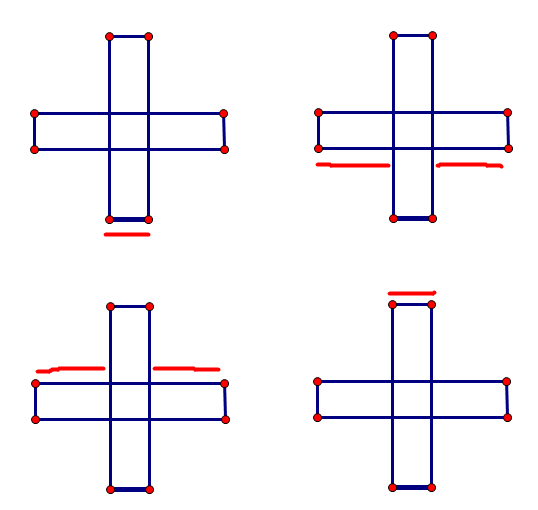
\includegraphics[scale=0.50]{./images/scan_line.png} % 插入图片
\end{figure}

\begin{lstlisting}
#include <bits/stdc++.h>
using namespace std;
const int N = 1e5 + 10;
int n;

namespace RectangularPerimeterUnion {
	int cor[2][N][2], m;
	struct E {
		int l, r, h, d;
		E() {}
		E(int l, int r, int h, int d) : l(l), r(r), h(h), d(d) {}
		bool operator < (const E &other) const { if (h != other.h) return h < other.h; return d > other.d; }
	}e[N << 1];
	struct Hash {
		vector <int> a;
		int operator[](int x) { return a[x - 1]; }
		int size() { return a.size(); }
		void init() { a.clear(); }
		void add(int x) { a.push_back(x); }
		void gao() { sort(a.begin(), a.end()); a.erase(unique(a.begin(), a.end()), a.end()); }
		int get(int x) { return lower_bound(a.begin(), a.end(), x) - a.begin() + 1; }	
	}hs;
	struct SEG {
		struct node {
			int cnt, len;
			node() { cnt = len = 0; }
		}t[N << 2];
		void build(int id, int l, int r) {
			t[id] = node();
			if (l == r) return;
			int mid = (l + r) >> 1;
			build(id << 1, l, mid);
			build(id << 1 | 1, mid + 1, r);
		}
		void up(int id, int l, int r) {
			if (t[id].cnt > 0) {
				t[id].len = hs[r] - hs[l - 1];
			} else {
				if (l == r) {
					t[id].len = 0;
				} else {
					t[id].len = t[id << 1].len + t[id << 1 | 1].len;
				}
			}
		}
		void update(int id, int l, int r, int ql, int qr, int v) {
			if (ql > qr) return;
			if (l >= ql && r <= qr) {
				t[id].cnt += v;
				up(id, l, r);
				return;
			}
			int mid = (l + r) >> 1;
			if (ql <= mid) update(id << 1, l, mid, ql, qr, v);
			if (qr > mid) update(id << 1 | 1, mid + 1, r, ql, qr, v);
			up(id, l, r);
		}
	}seg;
	int calc(int p) {
		hs.init();
		for (int i = 1; i <= n; ++i) {
			hs.add(cor[p][i][0]);
			hs.add(cor[p][i][1]);
		}
		hs.gao();
		m = 0;
		for (int i = 1; i <= n; ++i) {
			int l = hs.get(cor[p][i][0]);
			int r = hs.get(cor[p][i][1]);
			e[++m] = E(l + 1, r, cor[p ^ 1][i][0], 1);
			e[++m] = E(l + 1, r, cor[p ^ 1][i][1], -1);
		}
		sort(e + 1, e + 1 + m);
		int _n = hs.size();
		seg.build(1, 1, _n);
		int last = 0;
		int res = 0;
		for (int i = 1; i <= m; ++i) {
			int l = e[i].l, r = e[i].r;
			seg.update(1, 1, _n, l, r, e[i].d);
			int now = seg.t[1].len;
			res += abs(now - last);
			last = now;
		}
		return res;
	}
	int gao() {
		for (int i = 1; i <= n; ++i) {
			scanf("%d%d%d%d", &cor[0][i][0], &cor[1][i][0], &cor[0][i][1], &cor[1][i][1]);
		}
		return calc(0) + calc(1);
	}
}

int main() {
	while (scanf("%d", &n) != EOF) printf("%d\n", RectangularPerimeterUnion::gao());
    return 0;
}
\end{lstlisting}

只做一遍,同时维护竖线。

\begin{lstlisting}
#include <bits/stdc++.h>
using namespace std;
const int N = 1e5 + 10;
int n;

namespace RectangularPerimeterUnion {
	int m;
	struct E {
		int l, r, h, d;
		E() {}
		E(int l, int r, int h, int d) : l(l), r(r), h(h), d(d) {}
		bool operator < (const E &other) const { if (h != other.h) return h < other.h; return d > other.d; }
	}e[N << 1];
	struct Hash {
		vector <int> a;
		int operator[](int x) { return a[x - 1]; }
		int size() { return a.size(); }
		void init() { a.clear(); }
		void add(int x) { a.push_back(x); }
		void gao() { sort(a.begin(), a.end()); a.erase(unique(a.begin(), a.end()), a.end()); }
		int get(int x) { return lower_bound(a.begin(), a.end(), x) - a.begin() + 1; }	
	}hs; 
	struct SEG {
		struct node {
			int cnt, len, vtl, lbd, rbd;
			node() { cnt = len = vtl = lbd = rbd = 0; }
		}t[N << 2];
		void build(int id, int l, int r) {
			t[id] = node();
			if (l == r) return;
			int mid = (l + r) >> 1;
			build(id << 1, l, mid);
			build(id << 1 | 1, mid + 1, r);
		}
		void up(int id, int l, int r) {
			if (t[id].cnt > 0) {
				t[id].lbd = t[id].rbd = true;
				t[id].len = hs[r] - hs[l - 1];
				t[id].vtl = 2;
			} else {
				if (l == r) {
					t[id] = node();
				} else {
					t[id].lbd = t[id << 1].lbd;
					t[id].rbd = t[id << 1 | 1].rbd;
					t[id].len = t[id << 1].len + t[id << 1 | 1].len;
					t[id].vtl = t[id << 1].vtl + t[id << 1 | 1].vtl;
					if (t[id << 1].rbd && t[id << 1 | 1].lbd) t[id].vtl -= 2;
				}
			}
		}
		void update(int id, int l, int r, int ql, int qr, int v) {
			if (ql > qr) return;
			if (l >= ql && r <= qr) {
				t[id].cnt += v;
				up(id, l, r);
				return;
			}
			int mid = (l + r) >> 1;
			if (ql <= mid) update(id << 1, l, mid, ql, qr, v);
			if (qr > mid) update(id << 1 | 1, mid + 1, r, ql, qr, v);
			up(id, l, r);
		}
	}seg;
	int gao() {
		hs.init();
		m = 0;
		for (int i = 1; i <= n; ++i) {
			int x1, y1, x2, y2;
			scanf("%d%d%d%d", &x1, &y1, &x2, &y2);
			e[++m] = E(x1, x2, y1, 1);
			e[++m] = E(x1, x2, y2, -1);
			hs.add(x1);
			hs.add(x2);
		}
		hs.gao();
		sort(e + 1, e + 1 + m);
		int _n = hs.size();
		seg.build(1, 1, _n);
		int res = 0, last = 0;
		e[m + 1].h = 0;
		for (int i = 1; i <= m; ++i) {
			int l = hs.get(e[i].l) + 1;
			int r = hs.get(e[i].r);
			seg.update(1, 1, _n, l, r, e[i].d);
			res += seg.t[1].vtl * (e[i + 1].h - e[i].h);
			int now = seg.t[1].len;
			res += abs(now - last);
			last = now;
		}
		return res;
	}
}

int main() {
	while (scanf("%d", &n) != EOF) printf("%d\n", RectangularPerimeterUnion::gao());
    return 0;
}
\end{lstlisting}


\subsection{线段树合并与分裂}

时间复杂度:\par
$n$棵线段树初始有$O(n\log n)$的节点, 总点数就是$O(n \log n)$的\par
每次合并会将两个公共节点合并成一个,即删去一个节点,每个节点只会被删去一次, 所以时间复杂度为$O(n\log n)$\par

每一个分裂会产生$O(\log n)$个新节点\par
$m$次分裂最多产生$O(m\log n)$个新节点,所以即使降它们全部合并复杂度也只是$O(m\log n)$\par

Luogu P2824\par
题意:\par
给出一个$[1, n]$的排列, 进行$m$次局部排序。\par
\begin{itemize}
\item $0\;l\;r$, 将区间$[l, r]$进行升序排序
\item $1\;l\;r$, 将区间$[l, r]$进行降序排序
\end{itemize}

考虑排序可以用合并权值线段树来做,并且保存升/降序的标记即可。\par
那么区间排序,如果用$ODT$的思想用set维护区间,并且每次分裂只会分裂出$O(1)$个新区间,每个区间最多只会被合并一次,所以这部分复杂度为$O(m \log n)$\par
然后用线段树合并与分裂来维护set中每段区间对应的权值线段树。\par
这里能分裂是因为每个小区间都是有序的,分裂相当于分割出权值线段树的一段前缀或者后缀\par

\begin{lstlisting}
#include <bits/stdc++.h>
using namespace std;
const int N = 1e5 + 10;
int n, q, a[N];

struct SEG {
	struct node {
		int ls, rs, v;
		node() {}
		void init() { ls = rs = v = 0; }
	}t[N * 60];
	int tot;
	int newnode() { ++tot; t[tot].init(); return tot; }
	void init() { tot = 0; }
	void pushup(int id) { t[id].v = t[t[id].ls].v + t[t[id].rs].v; }
	void update(int &id, int l, int r, int pos, int v) {
		if (!id) id = newnode();
		if (l == r) {
			t[id].v += v;
			return;
		}
		int mid = (l + r) >> 1;
		if (pos <= mid) update(t[id].ls, l, mid, pos, v);
		else update(t[id].rs, mid + 1, r, pos, v);
		pushup(id);
	}
	void merge(int &x, int y, int l, int r) {
		if (!x || !y) { x |= y; return; }
		if (l == r) {
			t[x].v += t[y].v;
			return;
		}
		int mid = (l + r) >> 1;
		merge(t[x].ls, t[y].ls, l, mid);
		merge(t[x].rs, t[y].rs, mid + 1, r);
		pushup(x);
	}
	//k表示保存在y中的区间长度
	void split(int &x, int y, int k, int opt) {
		if (t[y].v == k) return;
		x = newnode();
		t[x].v = t[y].v - k;
		t[y].v = k;
		if (opt) {
			if (k <= t[t[y].rs].v) {
				split(t[x].rs, t[y].rs, k, opt);
				t[x].ls = t[y].ls;
				t[y].ls = 0;
			} else {
				split(t[x].ls, t[y].ls, k - t[t[y].rs].v, opt);
			}
		} else {
			if (k <= t[t[y].ls].v) {
				split(t[x].ls, t[y].ls, k, opt);
				t[x].rs = t[y].rs;
				t[y].rs = 0;
			} else {
				split(t[x].rs, t[y].rs, k - t[t[y].ls].v, opt);
			}
		}
	}
	//查找区间第k大
	int query(int id, int l, int r, int k, int opt) {
		if (l == r) return l;
		int mid = (l + r) >> 1;
		if (opt) {
			if (k <= t[t[id].rs].v) return query(t[id].rs, mid + 1, r, k, opt);
			else return query(t[id].ls, l, mid, k - t[t[id].rs].v, opt);
		} else {
			if (k <= t[t[id].ls].v) return query(t[id].ls, l, mid, k, opt);
			else return query(t[id].rs, mid + 1, r, k - t[t[id].ls].v, opt);
		}
	}
}seg;

struct ODT {
	//opt 0 升序 1 降序
	struct node {
		int l;
		mutable int r, segrt, opt;
		node() {}
		node(int l, int r = -1, int segrt = 0, int opt = 0) : l(l), r(r), segrt(segrt), opt(opt) {}
		bool operator < (const node &other) const { return l < other.l; }
	};
	using IT = set<node>::iterator;
	set <node> se;
	void init() { se.clear(); }
	IT split(int pos) {
		IT it = se.lower_bound(node(pos));
		if (it != se.end() && it->l == pos)
			return it;
		--it;
		int l = it->l, r = it->r, opt = it->opt, segrt = it->segrt, newsegrt; 
		seg.split(newsegrt, it->segrt, pos - it->l, opt);
		se.erase(it);
		se.insert(node(l, pos - 1, segrt, opt));
		return se.insert(node(pos, r, newsegrt, opt)).first;
	}
	void assign(int l, int r, int opt) {
		IT itr = split(r + 1), itl = split(l), it = itl;
		itl->opt = opt; 
		itl->r = r;
		for (++it; it != itr; ++it) {
			seg.merge(itl->segrt, it->segrt, 1, n);
		}
		it = itl; ++it;
		se.erase(it, itr);
	}
    int query(int pos) {
		IT it = se.upper_bound(node(pos)); --it; 
		return seg.query(it->segrt, 1, n, pos - it->l + 1, it->opt);
	}
}odt;

int main() {
	while (scanf("%d%d", &n, &q) != EOF) {
		for (int i = 1; i <= n; ++i) {
			scanf("%d", a + i);
		}
		seg.init();
		odt.init();
		for (int i = 1; i <= n; ++i) { 
			auto it = odt.se.insert(ODT::node(i, i, 0, 0)).first;
			seg.update(it->segrt, 1, n, a[i], 1);
		}
		for (int i = 1, op, l, r; i <= q; ++i) {
			scanf("%d%d%d", &op, &l, &r);
			odt.assign(l, r, op);
		}
		int x; scanf("%d", &x);
		printf("%d\n", odt.query(x));
	}
	return 0;
}
\end{lstlisting}

\subsection{势能线段树}

\subsubsection{HDU 5306}
HDU5306\par
题意:\par
三种操作:\par
\begin{itemize}
\item 将区间$[l_i, r_i]$内的数$a_i$变成$min(a_i, t)$\par
\item 输出区间最大值
\item 输出区间和
\end{itemize}

思路:\par
维护区间最大值和次大值, 以及最大值的个数:
\begin{itemize}
\item 如果更新值大于等于最大值那么不用往下更新
\item 如果更新值小于最大值大于次大值,那么直接更改最大值即可
\item 否则暴力往下更新
\end{itemize}
时间复杂度$O(n\log n)$

\begin{lstlisting}
#include <bits/stdc++.h>
using namespace std;
typedef long long ll;
const int N = 1e6 + 10, INF = 0x3f3f3f3f;
int n, q, a[N];

struct SEG {
	//+ < 取Min, 询问Max  - > 取Max, 询问Min 修改build初始化叶子结点
	static const int INF = 0x3f3f3f3f;
	static bool cmp(int x, int y) { return x < y; }
	static int get(int x, int y) { return cmp(x, y) ? y : x; }
	struct TAG {
		int v[2], cnt;
		TAG() {}
		void init() { v[0] = v[1] = -INF, cnt = 0;  } 
		TAG operator + (const TAG &other) const {
			TAG res; res.init();
			if (v[0] == other.v[0]) {
				res.v[0] = v[0];
				res.cnt = cnt + other.cnt;
				res.v[1] = get(v[1], other.v[1]);
			} else {
				if (cmp(v[0], other.v[0])) {
					res = other;
					res.v[1] = get(other.v[1], v[0]);
				} else {
					res = *this;
					res.v[1] = get(v[1], other.v[0]);
				}
			}	
			return res;
		}
	};
	struct node {
		ll sum; int lazy; 
	   	TAG tag; 
		node() { tag.init(); sum = 0; lazy = INF; }
		void up(int _lazy) {
		    if (cmp(_lazy, tag.v[0]) == 0) return; 
			sum += 1ll * tag.cnt * (_lazy - tag.v[0]); 
			tag.v[0] = _lazy;
			lazy = _lazy;
		}
		node operator + (const node &other) const {
			node res = node();
			res.sum = sum + other.sum; 
			res.tag = tag + other.tag;
			return res;
		}
	}t[N << 2], res; 
	void build(int id, int l, int r) {
		t[id] = node();
		if (l == r) {
			t[id].tag.cnt = 1;
			t[id].tag.v[0] = a[l];
			t[id].sum = a[l]; 
			return;
		}
		int mid = (l + r) >> 1;
		build(id << 1, l, mid);
		build(id << 1 | 1, mid + 1, r);
		t[id] = t[id << 1] + t[id << 1 | 1];
	}
	void pushdown(int id) {
		int &lazy = t[id].lazy;
		if (lazy == INF) return;
		t[id << 1].up(lazy);
		t[id << 1 | 1].up(lazy);
		lazy = INF;
	}
	void update(int id, int l, int r, int ql, int qr, int x) {
		if (cmp(x, t[id].tag.v[0]) == 0) return; 
		if (l == r) {
			x = cmp(x, t[id].tag.v[0]) ? x : t[id].tag.v[0];
			t[id].sum = x;
			t[id].tag.v[0] = x;
			t[id].tag.v[1] = -INF;
			return;
		} 
		if (l >= ql && r <= qr && cmp(x, t[id].tag.v[0]) && cmp(t[id].tag.v[1], x)) {
			t[id].up(x);
			return;
		}
		int mid = (l + r) >> 1;
		pushdown(id); 
		if (ql <= mid) update(id << 1, l, mid, ql, qr, x);
		if (qr > mid) update(id << 1 | 1, mid + 1, r, ql, qr, x);
		t[id] = t[id << 1] + t[id << 1 | 1];
	}
	void query(int id, int l, int r, int ql, int qr) {
		if (l >= ql && r <= qr) {
			res = res + t[id];
			return;
		}
		int mid = (l + r) >> 1;
		pushdown(id);
		if (ql <= mid) query(id << 1, l, mid, ql, qr);
		if (qr > mid) query(id << 1 | 1, mid + 1, r, ql, qr);
	}
}seg;

int main() {
	int T; scanf("%d", &T);
	while (T--) {
		scanf("%d%d", &n, &q);
		for (int i = 1; i <= n; ++i) {
			scanf("%d", a + i);
		}
		seg.build(1, 1, n);
		int op, x, y, t;
		while (q--) {
			scanf("%d%d%d", &op, &x, &y);
			if (!op) {
				scanf("%d", &t);
				seg.update(1, 1, n, x, y, t);
			} else {
				seg.res = SEG::node();
				seg.query(1, 1, n, x, y);
				printf("%lld\n", (op == 1 ? seg.res.tag.v[0] : seg.res.sum));
			}
		}
	}
	return 0;
}
\end{lstlisting}

\subsection{李超线段树}
\textbf{定义:}\par
支持动态维护一个平面直角坐标系,支持在中间插入一条线段或者直线,支持询问与$x = k$这条直线相交的所有线段中,交点的$y$轴坐标的最值\par
\textbf{维护什么?}\par
维护这个区间内的所有直线中,从上往下能够看到的最长的那个线段,也就是没有被其他直线覆盖长度最长的段\par
\textbf{怎么插入?}\par
\begin{itemize}
\item 如果这个区间没有记录最长的线段,那么直接把这个区间记录的线段修改为这条线段,然后返回。
\item 如果当前线段在这个区间内已经被这个区间内的最长线段为覆盖,那么直接返回。
\item 反过来,如果完全覆盖了之前记录的线段,那么直接赋值、返回。
\item 否则和已经记录的直线有交,判断哪根线段覆盖的区域较长,把这个区间记录的值给修改一下,然后把短的那一半丢下去递归。
\end{itemize} \par
\textbf{复杂度?}\par
每次递归下去直线的长度至少减少一半,复杂度为一个$log$。 \par
如果是插入线段,要先找到对应的区间插入,复杂度是两个$log$。\par

\subsubsection{插入直线}
BZOJ 1568
\begin{lstlisting}
#include <bits/stdc++.h>
using namespace std;
typedef double db;
const db eps = 1e-8;
int sgn(db x) { if (fabs(x) < eps) return 0; return x < 0 ? -1 : 1; }
const int N = 5e4 + 10;
#define N 50010
int n, q;

struct SEG {
	struct node {
		bool F; db k, b; 
		node(bool F = 0, db k = 0, db b = 0) : F(F), k(k), b(b) {}
		db calc(db x) { return k * x + b; }
	}t[N << 2];
	void build(int id, int l, int r) {
		t[id] = node();
		if (l == r) return;
		int mid = (l + r) >> 1;
		build(id << 1, l, mid);
		build(id << 1 | 1, mid + 1, r);
	}
	db div(db a, db b) { return a / b; }
//	db div(db a, db b) { return a / b - ((a ^ b) < 0 && a % b); }
	void update(int id, int l, int r, node tmp) { 
		if (t[id].F == 0) {
			t[id] = tmp; 
			return;
		}
		int mid = (l + r) >> 1;
		db preL = t[id].calc(l), preR = t[id].calc(r);
		db newL = tmp.calc(l), newR = tmp.calc(r);
		//维护最大值优势线段
		if (sgn(preL - newL) >= 0 && sgn(preR - newR) >= 0) return;
		if (newL > preL && newR > preR) {
			t[id] = tmp;
			return;
		}
		//计算交点
		db x = div(tmp.b - t[id].b, t[id].k - tmp.k);
		if (newL > preL) { 
			if (x > mid) {
				update(id << 1 | 1, mid + 1, r, t[id]); 
				t[id] = tmp;
			} else {
				update(id << 1, l, mid, tmp); 
			}
		} else {
			if (x > mid) {
				update(id << 1 | 1, mid + 1, r, tmp);
			} else {
				update(id << 1, l, mid, t[id]);
				t[id] = tmp;
			}
		}
	}
	void update(int id, int l, int r, db k, db b) { update(id, l, r, node(1, k, b)); }
	db query(int id, int l, int r, int x) {
		if (l == r) return t[id].calc(x);
		int mid = (l + r) >> 1;
		db res = t[id].calc(x);
		if (x <= mid) res = max(res, query(id << 1, l, mid, x));
		else res = max(res, query(id << 1 | 1, mid + 1, r, x));
		return res;
	}
}seg;

int main() {
	n = 50000;
	while (scanf("%d", &q) != EOF) {
		seg.build(1, 1, n);
		char op[20]; db k, b; int x;
		for (int _q = 1; _q <= q; ++_q) {
			scanf("%s", op + 1);
			switch(op[1]) {
				case 'P' :
					scanf("%lf%lf", &b, &k);
					seg.update(1, 1, n, k, b - k);
					break;
				case 'Q' :
					scanf("%d\n", &x);
					printf("%lld\n", (long long)(seg.query(1, 1, n, x) / 100));
					break;
			}
		}	
	}
	return 0;
}
\end{lstlisting}

\subsubsection{插入线段}
BZOJ 3165 LOJ 6034\par
更新复杂度$O(\log^2 n)$, 查询复杂度$O(\log n)$\par
\begin{lstlisting}
#include <bits/stdc++.h>
using namespace std;
typedef double db;
const int N = 1e5 + 10;
const db eps = 1e-8;
int sgn(db x) { if (fabs(x) < eps) return 0; return x < 0 ? -1 : 1; }
int q, ans, tot;
db K[N], B[N];
struct SEG { 
	struct node {
		db k, b; int pos; 
		bool F;
		node(db k = 0, db b = 0, int pos = 0, bool F = 0) : k(k), b(b), pos(pos), F(F) {}
		db calc(db x) { return k * x + b; }
	}t[N << 2];
	void build(int id, int l, int r) {
		t[id] = node();
		if (l == r) return;
		int mid = (l + r) >> 1;
		build(id << 1, l, mid);
		build(id << 1 | 1, mid + 1, r);
	}
	db div(db a, db b) { return a / b; }
//	db div(db a, db b) { return a / b - ((a ^ b) < 0 && a % b); }
	void update(int id, int l, int r, node tmp) { 
		if (t[id].F == 0) {
			t[id] = tmp;
			return;
		}
		int mid = (l + r) >> 1;
		db preL = t[id].calc(l), preR = t[id].calc(r);
		db newL = tmp.calc(l), newR = tmp.calc(r);
		if (sgn(preL - newL) >= 0 && sgn(preR - newR) >= 0) return;
		if (newL > preL && newR > preR) {
			t[id] = tmp;
			return;
		}
		db x = div(tmp.b - t[id].b, t[id].k - tmp.k);
		if (newL > preL) { 
			if (x > mid) {
				update(id << 1 | 1, mid + 1, r, t[id]); 
				t[id] = tmp;
			} else {
				update(id << 1, l, mid, tmp); 
			}
		} else {
			if (x > mid) {
				update(id << 1 | 1, mid + 1, r, tmp);
			} else {
				update(id << 1, l, mid, t[id]);
				t[id] = tmp;
			}
		}
	}
	void update(int id, int l, int r, int ql, int qr, node tmp) {
		if (l >= ql && r <= qr) {
			update(id, l, r, tmp);
			return;
		}
		int mid = (l + r) >> 1;
		if (ql <= mid) update(id << 1, l, mid, ql, qr, tmp);
		if (qr > mid) update(id << 1 | 1, mid + 1, r, ql, qr, tmp);
	}
	void update(int id, int l, int r, int ql, int qr, db k, db b, int pos) { update(id, l, r, ql, qr, node(k, b, pos, 1)); }
	void Cmax(int &a, int b, int x) { 
		db ya = K[a] * x + B[a];
		db yb = K[b] * x + B[b];
		if (ya < yb || (fabs(ya - yb) < eps && a > b)) a = b; 
	}
	int query(int id, int l, int r, int x) {
		if (l == r) return t[id].pos;
		int mid = (l + r) >> 1;
		int res = t[id].pos;
		if (x <= mid) Cmax(res, query(id << 1, l, mid, x), x);
		else Cmax(res, query(id << 1 | 1, mid + 1, r, x), x);
		return res;
	}
}seg;

int main() {
	while(scanf("%d", &q) != EOF) {
		int n = 100000;
		seg.build(1, 1, n);
		int op, x[2], y[2];
		int mod = 39989;
		ans = 0;
		for (int _q = 1; _q <= q; ++_q) {
			scanf("%d", &op);
			switch(op) {
				case 0 :
					scanf("%d", x);
					x[0] = (x[0] + ans - 1) % mod + 1;
					printf("%d\n", ans = seg.query(1, 1, n, x[0]));
					break;
				case 1 :
					for (int i = 0; i < 2; ++i) {
						scanf("%d%d", x + i, y + i);
						x[i] = (x[i] + ans - 1) % mod + 1;
						y[i] = (y[i] + ans - 1) % 1000000000 + 1;
					}
					if (x[0] > x[1]) {
						swap(x[0], x[1]);
						swap(y[0], y[1]);
					}
					++tot;
					K[tot] = 1.0 * (y[0] - y[1]) / (x[0] - x[1]);
					B[tot] = y[0] - K[tot] * x[0];
					seg.update(1, 1, n, x[0], x[1], K[tot], B[tot], tot);
					break;
			}
		}
	} 
	return 0;
}
\end{lstlisting}


\subsection{历史最值线段树}

BZOJ 3064\par
题意:\par
\begin{itemize}
\item $Q\;x\;y$, 查询$[x, y]$之间的历史最大值
\item $A\;x\;y$, 查询$[x, y]$之间的最大值
\item $P\;x\;y\;z$, 使得$[x, y]$之间的$a_i = a_i + z$
\item $C\;x\;y\;z$, 使得$[x, y]$之间的$a_i = z$
\end{itemize}

思路:\par
定义标记$(a, b)$为$A_i = max(A_i + a, b)$\par
区间加操作等价于标记$(a, -\infty)$, 区间赋值操作等价于$(-\infty, a)$\par
两个标记合并:$(a, b) + (c, d) = (a + c, max(b + c, d))$\par
两个标记取最大值:$(a, b) * (c, d) = (max(a, c), max(b, d))$\par

维护当前最大值,当前标记,历史最大值,历史标记最大值即可\par

\begin{lstlisting}
#include <bits/stdc++.h>
using namespace std;
typedef long long ll;
const int N = 1e5 + 10;
int n, q, a[N];

struct SEG {
	const static ll INF = 0x3f3f3f3f3f3f3f3f;
	struct TAG {
		ll a, b;
		TAG() {}
		TAG(ll a, ll b) : a(a), b(b) {}
		void init() { a = 0, b = -INF; }
		TAG operator + (const TAG &other) { return {max(-INF, a + other.a), max(b + other.a, other.b)}; } 
		TAG operator * (const TAG &other) { return {max(a, other.a), max(b, other.b)}; } 
		ll calc(ll x) { return max(x + a, b); }
	};
	struct node {
		ll v, hv; 
		TAG lazy, hlazy;
		node() {}
		void init() { v = hv = -INF; lazy.init(); hlazy.init(); }
		void up(TAG _lazy, TAG _hlazy) {
			hlazy = hlazy * (lazy + _hlazy);
			lazy = lazy + _lazy;
			hv = max(hv, _hlazy.calc(v));
			v = _lazy.calc(v);
		}
		node operator + (const node &other) const {
			node res; res.init();
			res.v = max(v, other.v);
			res.hv = max(hv, other.hv);
			return res;
		}
	}t[N << 2], res;
	void pushdown(int id) {
		TAG &lazy = t[id].lazy, &hlazy = t[id].hlazy;
		t[id << 1].up(lazy, hlazy);
		t[id << 1 | 1].up(lazy, hlazy);
		lazy.init(); hlazy.init();
	}
	void build(int id, int l, int r) {
		t[id].init();
		if (l == r) {
			t[id].v = t[id].hv = a[l];
			return;
		}
		int mid = (l + r) >> 1;
		build(id << 1, l, mid);
		build(id << 1 | 1, mid + 1, r);
		t[id] = t[id << 1] + t[id << 1 | 1];
	}
	void update(int id,int l, int r, int ql, int qr, TAG v) {
		if (l >= ql && r <= qr) {
			t[id].up(v, v);
			return;
		}
		int mid = (l + r) >> 1;
		pushdown(id);
		if (ql <= mid) update(id << 1, l, mid, ql, qr, v);
		if (qr > mid) update(id << 1 | 1, mid + 1, r, ql, qr, v);
		t[id] = t[id << 1] + t[id << 1 | 1];
	}
	void query(int id, int l, int r, int ql, int qr) {
		if (l >= ql && r <= qr) {
			res = res + t[id];
			return;
		}
		int mid = (l + r) >> 1;
		pushdown(id);
		if (ql <= mid) query(id << 1, l, mid, ql, qr);
		if (qr > mid) query(id << 1 | 1, mid + 1, r, ql, qr);
	}
}seg;

int main() {
	while (scanf("%d", &n) != EOF) {
		for (int i = 1; i <= n; ++i) scanf("%d", a + i);
		seg.build(1, 1, n);
		scanf("%d", &q);
		char op[10];
		for (int _q = 1, x, y, z; _q <= q; ++_q) {
			scanf("%s%d%d", op, &x, &y);
			if (op[0] == 'Q') {
				seg.res.init();
				seg.query(1, 1, n, x, y);
				printf("%lld\n", seg.res.v);
			} else if (op[0] == 'A') {
				seg.res.init();
				seg.query(1, 1, n, x, y);
				printf("%lld\n", seg.res.hv);
			} else if (op[0] == 'P') {
				scanf("%d", &z);
				seg.update(1, 1, n, x, y, SEG::TAG(z, -SEG::INF)); 
			} else if (op[0] == 'C') {
				scanf("%d", &z);
				seg.update(1, 1, n, x, y, SEG::TAG(-SEG::INF, z));
			}
		}
	}
	return 0;
}
\end{lstlisting}

\subsection{线段树维护立方和}
HDU 4578\par
题意:\par
\begin{itemize}
\item 区间加
\item 区间乘
\item 区间赋值
\item 给出$l, r, p(1 \leq p \leq 3)$, 询问$\sum\limits_{i = l}^r a_i^p$
\end{itemize} \par

\begin{lstlisting}
#include <bits/stdc++.h>
using namespace std;
const int N = 1e5 + 10, mod = 1e4 + 7;
int n, q;
struct SEG {
	struct node {
		int l, r;
		int sum[3], lazy[3]; 
		node() {} 
		node(int _l, int _r) {
			l = _l, r = _r;
			memset(sum, 0, sizeof sum);
			lazy[0] = 0, lazy[1] = 1, lazy[2] = -1; 
		}
	}t[N << 2];
	void pushup(int id) {
		for (int i = 0; i < 3; ++i) {
			t[id].sum[i] = (t[id << 1].sum[i] + t[id << 1 | 1].sum[i]) % mod;
		}
	}
	//add
	void work1(node &r, int b) {
		int len = r.r - r.l + 1;  
		r.sum[2] = (r.sum[2] + (len * b % mod * b % mod * b % mod) + (3 * b % mod * b % mod * r.sum[0] % mod) + (3 * b % mod * r.sum[1] % mod)) % mod;
		r.sum[1] = (r.sum[1] + (2 * b % mod * r.sum[0] % mod) + (len * b % mod * b % mod)) % mod;
		r.sum[0] = (r.sum[0] + len * b % mod) % mod;
		r.lazy[0] = (r.lazy[0] + b) % mod; 
	} 
	//mul
	void work2(node &r, int b) {
		r.sum[0] = (r.sum[0] * b) % mod;
		r.sum[1] = (r.sum[1] * b % mod * b) % mod;
		r.sum[2] = (r.sum[2] * b % mod * b % mod * b) % mod;
		r.lazy[0] = r.lazy[0] * b % mod;
		r.lazy[1] = r.lazy[1] * b % mod;
	} 
	//change
	void work3(node &r, int b) {
		int len = r.r - r.l + 1;
		r.sum[0] = len * b % mod;
		r.sum[1] = r.sum[0] * b % mod;
		r.sum[2] = r.sum[1] * b % mod; 
		r.lazy[0] = 0; r.lazy[1] = 1;  
		r.lazy[2] = b;   
	} 
	void pushdown(int id) {
		if (t[id].l >= t[id].r) return; 
		if (~t[id].lazy[2]) {
			work3(t[id << 1], t[id].lazy[2]);
			work3(t[id << 1 | 1], t[id].lazy[2]); 
			t[id].lazy[2] = -1;  
		}
		if (t[id].lazy[1] != 1) {
			work2(t[id << 1], t[id].lazy[1]);
			work2(t[id << 1 | 1], t[id].lazy[1]);
			t[id].lazy[1] = 1; 
		}
		if (t[id].lazy[0]) {
			work1(t[id << 1], t[id].lazy[0]);
			work1(t[id << 1 | 1], t[id].lazy[0]);
			t[id].lazy[0] = 0; 
		}
	}
	void build(int id, int l, int r) {
		t[id] = node(l, r);
		if (l == r) return;
		int mid = (l + r) >> 1;
		build(id << 1, l, mid);
		build(id << 1 | 1, mid + 1, r);
	}
	void update(int id, int l, int r, int vis, int val) {
		if (t[id].l >= l && t[id].r <= r) {
			if (vis == 1) work1(t[id], val); 
			else if (vis == 2) work2(t[id], val);
			else work3(t[id], val);   
			return;  
		}
		pushdown(id); 
		int mid = (t[id].l + t[id].r) >> 1;
		if (l <= mid) update(id << 1, l, r, vis, val);
		if (r > mid) update(id << 1 | 1, l, r, vis, val);  
		pushup(id);
	}
	int query(int id, int l, int r, int p) {
		if (t[id].l >= l && t[id].r <= r) return t[id].sum[p]; 
		int res = 0;
		pushdown(id); 
		int mid = (t[id].l + t[id].r) >> 1;
		if (l <= mid) res = (res + query(id << 1, l, r, p)) % mod; 
		if (r > mid) res = (res + query(id << 1 | 1, l, r, p)) % mod; 
		return res;
	}
}seg;

int main() {
	while (scanf("%d%d", &n, &q), n || q) {
		seg.build(1, 1, n);
		for (int i = 1, op, x, y, c; i <= q; ++i) {
			scanf("%d%d%d%d", &op, &x, &y, &c);
			if (op <= 3) seg.update(1, x, y, op, c); 
			else printf("%d\n", seg.query(1, x, y, c - 1));
		}
	}
	return 0;
}
\end{lstlisting}

\subsection{可持久化区间线段树}
SPOJ-TTM\par
给出一个序列$a_i$,维护四种操作:\par
\begin{itemize}
\item $C\;l\;r\;d$, 将$a_i, i \in [l, r]$加上$d$,并且使当前时间戳$+1$
\item $Q\;l\;r$, 查询当前版本$\sum\limits_{i = l}^r a_i$
\item $H\;l\;r\;t$, 查询时间戳为$t$的版本的$\sum\limits_{i = l}^r a_i$
\item $B\;t$,回到时间戳$t$
\end{itemize}

可持久化区间线段树不能用$pushdown$和$pushup$,因为$pushdown$的时候那些儿子是旧版本中的儿子,$down$下去后应该变成新版本的,但是各种版本的$lazy$标记打在一个点上的时候就没法处理了。\par
使用标记永久化,对于当前点以及其祖先的贡献直接在$update$过程中更新好,对于它孩子的贡献,直接在那个点处打个标记,查询的时候加上即可。\par

\begin{lstlisting}
#include <bits/stdc++.h>
using namespace std; 
using ll = long long;
const int N = 1e5 + 10;
int n, q, a[N], rt[N]; 

struct SEG {
	struct node {
		int ls, rs;
		ll lazy, sum;
		node() { ls = rs = lazy = sum = 0; }
	}t[N * 40];
	int tot;
	int newnode() { ++tot; t[tot] = node();  return tot; }
	void init() { tot = 0; }
	void build(int &id, int l, int r) {
		if (!id) id = newnode();
		if (l == r) {
			t[id].sum = a[l];
			return;
		}
		int mid = (l + r) >> 1;
		build(t[id].ls, l, mid);
		build(t[id].rs, mid + 1, r);
		t[id].sum = t[t[id].ls].sum + t[t[id].rs].sum;
	}
	void update(int &now, int pre, int l, int r, int ql, int qr, ll v) {
		now = newnode();
		t[now] = t[pre];
		t[now].sum += v * (min(r, qr) - max(l, ql) + 1);
		if (l >= ql && r <= qr) {
			t[now].lazy += v;
			return;
		}
		int mid = (l + r) >> 1;
		if (ql <= mid) update(t[now].ls, t[pre].ls, l, mid, ql, qr, v);
		if (qr > mid) update(t[now].rs, t[pre].rs, mid + 1, r, ql, qr, v);
	}
	ll query(int id, int l, int r, int ql, int qr) {
		if (ql > qr) return 0;
		if (l >= ql && r <= qr) return t[id].sum;
		int mid = (l + r) >> 1;
		ll res = t[id].lazy * (min(r, qr) - max(l, ql) + 1);
		if (ql <= mid) res += query(t[id].ls, l, mid, ql, qr);
		if (qr > mid) res += query(t[id].rs, mid + 1, r, ql, qr);
		return res;
	}
}seg;

int main() {
	while (scanf("%d%d", &n, &q) != EOF) {
		for (int i = 1; i <= n; ++i) scanf("%d", a + i); 
		seg.init();
		seg.build(rt[0], 1, n);
		int cntrt = 0;
		char op; int l, r, t; ll d; 
		for (int i = 1; i <= q; ++i) {
			scanf(" %c", &op);
			if (op == 'C') {
				scanf("%d%d%lld", &l, &r, &d); 
				++cntrt;
				rt[cntrt] = rt[cntrt - 1];
				seg.update(rt[cntrt], rt[cntrt], 1, n, l, r, d);
			} else if (op == 'Q') {
				scanf("%d%d", &l, &r);
				printf("%lld\n", seg.query(rt[cntrt], 1, n, l, r));
			} else if (op == 'H') {
				scanf("%d%d%d", &l, &r, &t);
				printf("%lld\n", seg.query(rt[t], 1, n, l, r));
			} else {
				scanf("%d", &t);
				cntrt = t;
			}
		}
	}
	return 0;
}
\end{lstlisting}

\subsection{区间线段树套区间线段树}
Luogu P3437\par
题意:\par
查询矩形区间最大值,更新矩形区间最大值\par
思路: \par
区间线段树套区间线段树,建树复杂度$O(n^2)$,直接暴力建树即可,如果有初始值就暴力遍历取$max$即可,更新和查询复杂度$O(\log^2n)$。\par
但是考虑到$pushup$的复杂度是不对的,所以不要$pushup$,直接用标记永久化。\par
内存不够可以尝试开两倍或者三倍内存,不一定要开四倍,因为单棵线段树长度比较小。\par

\begin{lstlisting}
#include <bits/stdc++.h>
using namespace std;
const int N = 1e3 + 5;
int n, m, q;

struct ODTree {
	struct node {
		int Max, lazy; 
		node() {};
		void init() { Max = lazy = 0; }
	}t[N * 3];
	void build(int id, int l, int r, int Tl, int Tr) {
		t[id].init();
		if (l == r) return;
		int mid = (l + r) >> 1;
		build(id << 1, l, mid, Tl, Tr);
		build(id << 1 | 1, mid + 1, r, Tl, Tr); 
	}
	void update(int id, int l, int r, int ql, int qr, int v) {
		if (min(r, qr) - max(l, ql) + 1 > 0) {
			t[id].Max = max(t[id].Max, v);
		}
		if (l >= ql && r <= qr) {
			t[id].lazy = max(t[id].lazy, v);
			return;
		}
		int mid = (l + r) >> 1;
		if (ql <= mid) update(id << 1, l, mid, ql, qr, v);
		if (qr > mid) update(id << 1 | 1, mid + 1, r, ql, qr, v);
	}	
	int query(int id, int l, int r, int ql, int qr) {
		if (l >= ql && r <= qr) return t[id].Max;
		int mid = (l + r) >> 1;
		int res = t[id].lazy;
		if (ql <= mid) res = max(res, query(id << 1, l, mid, ql, qr));
		if (qr > mid) res = max(res, query(id << 1 | 1, mid + 1, r, ql, qr));
		return res;	
	}
};

struct TDTree {
	struct node {
		ODTree Max, lazy;
		node() {}
	}t[N * 3];
	void build(int id, int l, int r) {
		t[id].Max.build(1, 1, m, l, r);
		t[id].lazy.build(1, 1, m, l, r);
		if (l == r) return;
		int mid = (l + r) >> 1;
		build(id << 1, l, mid);
		build(id << 1 | 1, mid + 1, r);
	}
	void update(int id, int l, int r, int ql, int qr, int Ol, int Or, int v) {
		if (min(r, qr) - max(l, ql) + 1 > 0) {
			t[id].Max.update(1, 1, m, Ol, Or, v);
		}
		if (l >= ql && r <= qr) {
			t[id].lazy.update(1, 1, m, Ol, Or, v);
			return;
		}
		int mid = (l + r) >> 1;
		if (ql <= mid) update(id << 1, l, mid, ql, qr, Ol, Or, v);
		if (qr > mid) update(id << 1 | 1, mid + 1, r, ql, qr, Ol, Or, v);
	}
	int query(int id, int l, int r, int ql, int qr, int Ol, int Or) {
		if (l >= ql && r <= qr) return t[id].Max.query(1, 1, m, Ol, Or);
		int mid = (l + r) >> 1;
		int res = t[id].lazy.query(1, 1, m, Ol, Or);
		if (ql <= mid) res = max(res, query(id << 1, l, mid, ql, qr, Ol, Or));
		if (qr > mid) res = max(res, query(id << 1 | 1, mid + 1, r, ql, qr, Ol, Or));
		return res;
	}
}td;

int main() {
	while (scanf("%d%d%d", &n, &m, &q) != EOF) {
		++n, ++m;
		td.build(1, 1, n);
		for (int i = 1, d, s, w, x, y; i <= q; ++i) {
			scanf("%d%d%d%d%d", &d, &s, &w, &x, &y);
			td.update(1, 1, n, x + 1, x + d, y + 1, y + s, td.query(1, 1, n, x + 1, x + d, y + 1, y + s) + w);
		} 
		printf("%d\n", td.query(1, 1, n, 1, n, 1, m));
	}
	return 0;
}
\end{lstlisting}

\subsection{区间线段树套权值线段树}
牛客 3979I\par
题意:\par
一个序列,维护两种操作:\par
\begin{itemize}
\item $1\;l\;r\;x$, 对$i \in [l, r]$,令$A_i = min(A_i, x)$
\item $2\;l\;r\;k$,询问$[l, r]$中第$k$小的数字
\end{itemize} \par
思路:\par
考虑区间线段树上的每一个节点$[l, r]$,可以用一个动态开点权值线段树记录$[l, r]$中每种权值出现了多少次。\par
询问可以转化成在$O(logn)$棵线段树上二分,询问复杂度$o(log^2n)$。\par
修改的时候,定位到一些节点$[l_i, r_i]$,将所有$> x$的数都并到$x$处,主要要将$[l_i, r_i]$及其祖先的内层线段树都要操作,时间复杂度$O(tlog^2n)$,$t$为合并的节点数。\par
然后打标记下传即可,注意$pushdown$的时候不需要更新祖先的内层线段树,因为已经更新过了。\par
每个节点只会被合并一次,一共有$O(nlogn)$个节点,所以总的时间复杂度$O(nlog^3n)$\par
\begin{lstlisting}
#include <bits/stdc++.h>
using namespace std;
const int N = 8e4 + 10;
int n, q, a[N];
 
struct VSEG {
    struct node {
        int sum, Max, ls, rs;
        node() {}
        void init() {
            sum = Max = 0;
            ls = rs = 0;
        }
    }t[N * 400];
    int cnt = 0;
    void init() { cnt = 0; }
    int newnode() {
        ++cnt;
        t[cnt].init();
        return cnt;
    }
    void up(int id) {
        int ls = t[id].ls, rs = t[id].rs;
        t[id].sum = t[ls].sum + t[rs].sum;
        t[id].Max = max(t[ls].Max, t[rs].Max);
    }
    void update(int id, int l, int r, int pos, int v) {
        if (l == r) {
            t[id].sum += v;
            if (t[id].sum) t[id].Max = pos;
            else t[id].Max = 0;
            return;
        }
        int mid = (l + r) >> 1;
        if (pos <= mid) {
            if (!t[id].ls) t[id].ls = newnode();
            update(t[id].ls, l, mid, pos, v);
        } else {
            if (!t[id].rs) t[id].rs = newnode();
            update(t[id].rs, mid + 1, r, pos, v);
        }
        up(id);
    }
    int query(int id, int l, int r, int pos) {
        if (!id) return 0;
        if (l == r) return t[id].sum;
        int mid = (l + r) >> 1;
        if (pos <= mid) return query(t[id].ls, l, mid, pos);
        else return query(t[id].rs, mid + 1, r, pos);
    }
}vseg;
 
struct SEG {
    struct node {
        int id, lazy, l, r;
        node() {}
        void init() {
            id = l = r = 0;
        }
    }t[N << 2];
    vector <int> vec;
    void build(int id, int l, int r) {
        t[id].l = l; t[id].r = r;
        t[id].id = vseg.newnode();
        for (int i = l; i <= r; ++i) {
            vseg.update(t[id].id, 1, n, a[i], 1);
        }
        t[id].lazy = n;
        if (l == r) {
            t[id].lazy = a[l];
            return;
        }
        int mid = (l + r) >> 1;
        build(id << 1, l, mid);
        build(id << 1 | 1, mid + 1, r);
    }
    void down(int id) {
        int &lazy = t[id].lazy;
        t[id << 1].lazy = min(lazy, t[id << 1].lazy);
        t[id << 1 | 1].lazy = min(lazy, t[id << 1 | 1].lazy);
        for (auto &it : {t[id << 1].id, t[id << 1 | 1].id}) {
            while (vseg.t[it].Max > lazy) {
                int pos = vseg.t[it].Max;
                int del = vseg.query(it, 1, n, pos);
                vseg.update(it, 1, n, pos, -del);
                vseg.update(it, 1, n, lazy, del);
            }
        }
    }
    void update(int id, int l, int r, int ql, int qr, int x) {
        if (l >= ql && r <= qr) {
            vector <int> vec;
            int it = id;
            while (it) {
                vec.push_back(t[it].id);
                it >>= 1;
            }
            while (vseg.t[t[id].id].Max > x) {
                int pos = vseg.t[t[id].id].Max;
                int del = vseg.query(t[id].id, 1, n, pos);
                for (auto &it : vec) {
                    vseg.update(it, 1, n, pos, -del);
                    vseg.update(it, 1, n, x, del);
                }
            }
            t[id].lazy = min(t[id].lazy, x);
            return;
        }
        int mid = (l + r) >> 1;
        down(id);
        if (ql <= mid) update(id << 1, l, mid, ql, qr, x);
        if (qr > mid) update(id << 1 | 1, mid + 1, r, ql, qr, x);
    }
    void add(int id, int l, int r, int ql, int qr) {
        if (l >= ql && r <= qr) {
            vec.push_back(t[id].id);
            return;
        }
        int mid = (l + r) >> 1;
        down(id);
        if (ql <= mid) add(id << 1, l, mid, ql, qr);
        if (qr > mid) add(id << 1 | 1, mid + 1, r, ql, qr);
    }
    int querygao(int l, int r, int k) {
        if (l == r) return l;
        int mid = (l + r) >> 1;
        int lsum = 0;
        for (auto &it : vec) lsum += vseg.t[vseg.t[it].ls].sum;
        if (lsum >= k) {
            for (auto &it : vec) it = vseg.t[it].ls;
            return querygao(l, mid, k);
        } else {
            for (auto &it : vec) it = vseg.t[it].rs;
            return querygao(mid + 1, r, k - lsum);
        }
    }
    int query(int l, int r, int k) {
        vec.clear();   
        add(1, 1, n, l, r);
        return querygao(1, n, k); 
    }
}seg;
 
int main() {
    while (scanf("%d%d", &n, &q) != EOF) {
        for (int i = 1; i <= n; ++i) scanf("%d", a + i);
        vseg.init();
        seg.build(1, 1, n);
        for (int _q = 1, tp, l, r, x; _q <= q; ++_q) {
            scanf("%d%d%d%d", &tp, &l, &r, &x);
            if (tp == 1) {
                if (x >= n) continue;
                seg.update(1, 1, n, l, r, x);
            } else {
                printf("%d\n", seg.query(l, r, x));
            }
        }
    }
    return 0;
}
\end{lstlisting}

\section{KD-Tree}

\subsection{Luogu P1429}

平面最近点对。\par

建树时的两个优化:
\begin{itemize}
\item 选择的维度要满足其内部点的分布的差异度最大,即每次选择的切割维度是方差最大的维度。
\item 每次在维度上选择切割点时选择该维度上的 中位数 ,这样可以保证每次分成的左右子树大小尽量相等。
\end{itemize}
使用优化$2$能够保证树高最多为$O(\log n)$。\par

查询的时候要用全局最优化剪枝\par

\begin{lstlisting}
#include <bits/stdc++.h>
using namespace std;
typedef double db;
const int N = 2e5 + 10;
const int K = 2;
const db INF = 0x3f3f3f3f3f3f3f3f;
int n; db ans;
inline db sqr(db x) { return x * x; }

struct Point {
	db x[K]; int id;
	db dis(const Point &b) const {
		db res = 0;
		for (int i = 0; i < K; ++i)
			res += sqr(x[i] - b.x[i]);
		return res;
	}
}s[N];

struct KDTree {
	struct cmpx {
		int div;
		cmpx(int div = 0) : div(div) {}
		bool operator () (const Point &a, const Point &b) {
			for (int i = 0; i < K; ++i)
				if (a.x[(i + div) % K] != b.x[(i + div) % K])
					return a.x[(i + div) % K] < b.x[(i + div) % K];
			return true;
		}
	};
	bool cmp(const Point &a, const Point &b, int div) { return cmpx(div)(a, b); }
	struct Node {
		Point e;
		db Min[K], Max[K]; 
		Node *ls, *rs;
		int div;
	}pool[N], *tail, *root;
	void init() { tail = pool; }
	void pushup(Node *a) {
		for (int i = 0; i < K; ++i) {
			a->Min[i] = a->Max[i] = a->e.x[i];
		}
	    if (a->ls) {
			for (int i = 0; i < K; ++i) {
				a->Min[i] = min(a->Min[i], a->ls->Min[i]);
				a->Max[i] = max(a->Max[i], a->ls->Max[i]);
			}
		}
		if (a->rs) {
			for (int i = 0; i < K; ++i) {
				a->Min[i] = min(a->Min[i], a->rs->Min[i]);
				a->Max[i] = max(a->Max[i], a->rs->Max[i]);
			}
		}
	}
	Node* build(int l, int r) {
		if (l > r) return nullptr;
		int mid = (l + r) >> 1;
		Node *p = tail++;
		p->div = 0;
		if (l == r) {
			p->e = s[mid];
			pushup(p);
			return p;
		}
		//average variance
		double avx[K] = {0}, vax[K] = {0};
		for (int i = l; i <= r; ++i) 
			for (int j = 0; j < K; ++j) 
				avx[j] += s[i].x[j];
		for (int i = 0; i < K; ++i) avx[i] /= (double)(r - l + 1);
		for (int i = l; i <= r; ++i) 
			for (int j = 0; j < K; ++j) 
				vax[j] += sqr(s[i].x[j] - avx[j]);
		for (int i = 1; i < K; ++i) {
			if (vax[i] > vax[p->div])
				p->div = i;
		}
		nth_element(s + l, s + mid, s + r + 1, cmpx(p->div));
		p->e = s[mid];
		p->ls = build(l, mid - 1);
		p->rs = build(mid + 1, r);
		pushup(p);
		return p;	
	}
	db calc(Node *a, Point &e) {
		if (a == nullptr) return INF; 
	    db res = 0;
		for (int i = 0; i < K; ++i) {
			if (a->Min[i] > e.x[i])
				res += sqr(a->Min[i] - e.x[i]);
			if (a->Max[i] < e.x[i])
				res += sqr(a->Max[i] - e.x[i]);
		}
		return res;
	}
	void query(Node *t, int l, int r, Point &e) {
	    if (l > r) return;
	    int mid = (l + r) >> 1;
	    if (t->e.id != e.id) ans = min(ans, e.dis(t->e));  
	    if (l == r) return;
	    db distl = calc(t->ls, e), distr = calc(t->rs, e);
	    if (distl < ans && distr < ans) {
	        if (distl < distr) {
	            query(t->ls, l, mid - 1, e);
	            if (distr < ans) query(t->rs, mid + 1, r, e);
	        } else {
	            query(t->rs, mid + 1, r, e);
	            if (distl < ans) query(t->ls, l, mid - 1, e); 
	        }
	    } else {
	        if (distl < ans) query(t->ls, l, mid - 1, e);
	        if (distr < ans) query(t->rs, mid + 1, r, e);
	    }
	}
}kdTree;

int main() {
    scanf("%d", &n);
    for (int i = 1; i <= n; i++) {
		scanf("%lf%lf", &s[i].x[0], &s[i].x[1]); 
		s[i].id = i;	
	}
	kdTree.init();
	kdTree.root = kdTree.build(1, n);
	ans = 2e18;
    for (int i = 1; i <= n; i++) kdTree.query(kdTree.root, 1, n, s[i]); 
    printf("%.4f\n", sqrt(ans));
    return 0;
}
\end{lstlisting}


\subsection{BZOJ 4520}

给出$n$个点,找欧式距离下的第$k$远点对。\par
点对为无序点对。\par
复杂度跟$k$有关,$k$不能太大。\par

\begin{lstlisting}
#include <bits/stdc++.h>
#define SZ(x) (int(x.size()))
using namespace std;
typedef long long db;
const int N = 1e5 + 10;
const int DIM = 2;
const int K = 2;
const db INF = 0x3f3f3f3f3f3f3f3f;
int n, k; 
inline db sqr(db x) { return x * x; }

struct Point {
	db x[DIM]; int id;
	void scan() { for (int i = 0; i < K; ++i) scanf("%lld", x + i); }
	void print() { for (int i = 0; i < K; ++i) printf("%lld%c", x[i], " \n"[i == K - 1]); }
	db dis(const Point &b) const {
		db res = 0;
		for (int i = 0; i < K; ++i)
			res += sqr(x[i] - b.x[i]); 
		return res;
	}
}s[N];

struct KDTree {
	struct cmpx {
		int div;
		cmpx(int div = 0) : div(div) {}
		bool operator () (const Point &a, const Point &b) {
			for (int i = 0; i < K; ++i)
				if (a.x[(i + div) % K] != b.x[(i + div) % K])
					return a.x[(i + div) % K] < b.x[(i + div) % K];
			return true;
		}
	};
	bool cmp(const Point &a, const Point &b, int div) { return cmpx(div)(a, b); }
	struct Node {
		Point e;
		db Min[DIM], Max[DIM];
		Node *ls, *rs;
		int div;
		void init() { ls = rs = NULL; div = 0;}
	}pool[N], *tail, *root;
	void init() { tail = pool; }
 	Node* newnode() { tail->init(); return tail++; }
	void pushup(Node *a) { 
		for (int i = 0; i < K; ++i) {
			a->Min[i] = a->Max[i] = a->e.x[i]; 
		} 
	    if (a->ls) {
			for (int i = 0; i < K; ++i) {
				a->Min[i] = min(a->Min[i], a->ls->Min[i]);
				a->Max[i] = max(a->Max[i], a->ls->Max[i]);
			}
		}
		if (a->rs) {
			for (int i = 0; i < K; ++i) {
				a->Min[i] = min(a->Min[i], a->rs->Min[i]);
				a->Max[i] = max(a->Max[i], a->rs->Max[i]);
			}
		}
	}
	Node* build(int l, int r, int div) {
		if (l > r) return NULL;
		int mid = (l + r) >> 1;
		Node *p = newnode();
		p->div = div;
		nth_element(s + l, s + mid, s + r + 1, cmpx(div));
		p->e = s[mid];
		p->ls = build(l, mid - 1, (div + 1) % K);
		p->rs = build(mid + 1, r, (div + 1) % K);
		pushup(p);
		return p;
	}	
	struct qnode {
		Point p;
		db dis;
		qnode() {}
		qnode(Point p, db dis) : p(p), dis(dis) {}
		bool operator < (const qnode &other) const { return dis > other.dis; }
	};
	priority_queue <qnode> pq;
	db calc(Node *t, Point e) {
		if (t == NULL) return 0;
		db res = 0;
		for (int i = 0; i < K; ++i) {
			res += max(sqr(e.x[i] - t->Max[i]), sqr(e.x[i] - t->Min[i]));
		}
		return res;
	}
	void search(Node *t, int k, Point p) {
		if (!t) return;
		if (!cmp(p, t->e, t->div)) {
			search(t->ls, k, p);	
			if (SZ(pq) < k) {
				if (p.id > t->e.id) pq.push(qnode(t->e, p.dis(t->e)));
				search(t->rs, k, p);
			} else {
				if (p.id > t->e.id && p.dis(t->e) > pq.top().dis) {
					pq.pop();
					pq.push(qnode(t->e, p.dis(t->e))); 
				} 
				if (calc(t->rs, p) > pq.top().dis)
					search(t->rs, k, p);
			}
		} else {
			search(t->rs, k, p);
			if (SZ(pq) < k) {
				if (p.id > t->e.id) pq.push(qnode(t->e, p.dis(t->e)));
				search(t->ls, k, p);
			} else {
				if (p.id > t->e.id && p.dis(t->e) > pq.top().dis) {
					pq.pop();
					pq.push(qnode(t->e, p.dis(t->e)));
				}
				if (calc(t->ls, p) > pq.top().dis)
					search(t->ls, k, p);
			}
		}
	}
}kdTree;

int main() {
	while (scanf("%d%d", &n, &k) != EOF) { 
		for (int i = 1; i <= n; ++i) {
			s[i].scan();
			s[i].id = i;
		}	
		kdTree.init();
		kdTree.root = kdTree.build(1, n, 0);
		for (int i = 1; i <= n; ++i) kdTree.search(kdTree.root, k, s[i]);
		printf("%lld\n", kdTree.pq.top().dis);
	}
    return 0;
}
\end{lstlisting}

\subsection{Luogu P4148}

单点加,矩形求和,强制在线,卡空间, 坐标范围$5 \cdot 10^5$, 操作次数$2 \cdot 10^5$\par


\textbf{查询流程:}
\begin{itemize}
\item 在查询矩形区域内的所有点的权值和时,仍然需要记录子树内每一维度上的坐标的最大值和最小值。如果当前子树对应的矩形与所求矩形没有交点,则不继续搜索其子树;
\item 如果当前子树对应的矩形完全包含在所求矩形内,返回当前子树内所有点的权值和;
\item 否则,判断当前点是否在所求矩形内,更新答案并递归在左右子树中查找答案。
\end{itemize}

插入操作直接暴力插入,用替罪羊思想重构即可。\par
如果有删除操作,直接打标记,有必要的话可以进行删除重构。\par

在$2D$树上进行矩阵查询, 已经被完全覆盖或者完全不相交的子树不会继续查询。\par
则单次查询时间复杂度最优是$O(\log n)$, 最坏是$O(\sqrt{n})$, 在$k$维的情况下, 最坏时间复杂度为$O(n^{1 - \frac{1}{k}})$的

\begin{lstlisting}
#include <bits/stdc++.h>
using namespace std;
typedef int db;
const int N = 2e5 + 10;
const int DIM = 2;
const int K = 2;

struct Point {
	db x[DIM]; int v;  
	bool In(db *Min, db *Max) {
		for (int i = 0; i < K; ++i) {
			if (x[i] < Min[i] || x[i] > Max[i])
				return 0;
		}
		return 1;
	}
}s[N]; int cntS; 

struct KDTree {
	static constexpr double alpha = 0.75;
	struct cmpx {
		int div;
		cmpx(int div = 0) : div(div) {}
		bool operator () (const int &a, const int &b) {
			return s[a].x[div] < s[b].x[div];
		}
	};
	bool cmp(const int &a, const int &b, const int &div) { return s[a].x[div] <= s[b].x[div]; }
	struct Node {
		int ls, rs, div;
		db Min[DIM], Max[DIM];
		int sze, sum;
		bool In(db *_Min, db *_Max) {
			for (int i = 0; i < K; ++i) {
				if (_Min[i] > Min[i] || _Max[i] < Max[i])
					return 0;
			}
			return 1;
		}
		bool Out(db *_Min, db *_Max) {
			for (int i = 0; i < K; ++i) {
				if (_Max[i] < Min[i] || _Min[i] > Max[i])
					return 1;
			}
			return 0;
		}
	}t[N]; 
	int root, g[N];
	void init() { root = 0; }
	void print(int o) {
	    if (!o) return;
	    print(t[o].ls);
	    g[++*g] = o;
	    print(t[o].rs);
	}
	void pushup(int o) {
	    t[o].sze = t[t[o].ls].sze + t[t[o].rs].sze + 1;
	    t[o].sum = t[t[o].ls].sum + t[t[o].rs].sum + s[o].v; 
		for (int i = 0; i < K; ++i) {
			t[o].Min[i] = t[o].Max[i] = s[o].x[i];
		}
	    if (t[o].ls) {
			for (int i = 0; i < K; ++i) {
				t[o].Min[i] = min(t[o].Min[i], t[t[o].ls].Min[i]);
				t[o].Max[i] = max(t[o].Max[i], t[t[o].ls].Max[i]);
			}
		}
	    if (t[o].rs) {
			for (int i = 0; i < K; ++i) {
				t[o].Min[i] = min(t[o].Min[i], t[t[o].rs].Min[i]);
				t[o].Max[i] = max(t[o].Max[i], t[t[o].rs].Max[i]);
			}
		}
	}
	int build(int l, int r) {
	    if (l > r) return 0;
	    int mid = (l + r) >> 1;
	    double ave[2] = {0}, vax[2] = {0};
	    for (int i = l; i <= r; i++) 
			for (int j = 0; j < K; ++j)
				ave[j] += s[g[i]].x[j];
		for (int i = 0; i < K; ++i) ave[i] /= (r - l + 1);
	    for (int i = l; i <= r; i++)
			for (int j = 0; j < K; ++j)
				vax[j] += (s[g[i]].x[j] - ave[j]) * (s[g[i]].x[j] - ave[j]);
		int div = 0;
		for (int i = 1; i < K; ++i) {
			if (vax[i] > vax[div])
				div = i;
		}
		nth_element(g + l, g + mid, g + r + 1, cmpx(div));
		int o = g[mid];
		t[o].div = div;
		t[o].ls = build(l, mid - 1);
		t[o].rs = build(mid + 1, r);
	    pushup(o);
	    return o;
	}
	void rebuild(int &o) {
	    *g = 0;
		print(o);
	    o = build(1, *g);
	}
	bool bad(int o) { return alpha * t[o].sze <= (double)max(t[t[o].ls].sze, t[t[o].rs].sze); } 
	void insert(int &o, int v) {
	    if (!o) {
	        o = v;
	        pushup(o);
	        return;
	    }
		if (cmp(v, o, t[o].div))
			insert(t[o].ls, v);
		else
			insert(t[o].rs, v);
	    pushup(o);
	    if (bad(o)) rebuild(o);
	}
	int query(int o, db *Min, db *Max) {
		if (!o || t[o].Out(Min, Max)) return 0;
		if (t[o].In(Min, Max)) return t[o].sum;
	    int res = 0;
		if (s[o].In(Min, Max)) res += s[o].v;
	    return query(t[o].ls, Min, Max) + query(t[o].rs, Min, Max) + res;
	}
}kdTree;

int main() {
	int n, op, ans = 0;
	db Min[DIM], Max[DIM];	
    scanf("%d", &n);
    while (scanf("%d", &op) != EOF) {
        if (op == 1) {
			++cntS;
            scanf("%d%d%d", &s[cntS].x[0], &s[cntS].x[1], &s[cntS].v);
            s[cntS].x[0] ^= ans;
            s[cntS].x[1] ^= ans;
            s[cntS].v ^= ans;
            kdTree.insert(kdTree.root, cntS);
        }
        if (op == 2) {
			for (int i = 0; i < K; ++i) scanf("%d", Min + i), Min[i] ^= ans;
			for (int i = 0; i < K; ++i) scanf("%d", Max + i), Max[i] ^= ans;
            printf("%d\n", ans = kdTree.query(kdTree.root, Min, Max));
        }
        if (op == 3) break;
    }
	return 0;
}
\end{lstlisting}

\subsection{BZOJ 2716}

每次插入一个点,或者给出一个点,询问已经被插入的点中和它曼哈顿距离最近的点的距离。\par

带插入平面最近点对加上信仰剪枝即可。\par

\begin{lstlisting}
#include <bits/stdc++.h>
using namespace std;
typedef int db;
const int N = 1e6 + 10;
const int DIM = 2;
const int K = 2;
const db INF = 0x3f3f3f3f;

struct Point {
	db x[DIM]; 
	void scan() { for (int i = 0; i < K; ++i) scanf("%d", x + i); }
	db dis(const Point &b) const {
		db res = 0;
		for (int i = 0; i < K; ++i)
			res += abs(x[i] - b.x[i]);  
		return res;
	}
}s[N]; int cntS; 

struct KDTree {
	#define alpha 0.725
	struct cmpx {
		int div;
		cmpx(int div = 0) : div(div) {} 
		bool operator () (const int &a, const int &b) {
			return s[a].x[div] < s[b].x[div];
		}
	};
	bool cmp(const int &a, const int &b, const int &div) { return s[a].x[div] <= s[b].x[div]; }
	struct Node {
		int ls, rs, div;
		db Min[DIM], Max[DIM];
		int sze;
	}t[N]; 
	int root, g[N];
	db ans;
	void init() { root = 0; }
	void print(int o) {
	    if (!o) return;
	    print(t[o].ls);
	    g[++*g] = o;
	    print(t[o].rs);
	}
	void pushup(int o) {
	    t[o].sze = t[t[o].ls].sze + t[t[o].rs].sze + 1;
		for (int i = 0; i < K; ++i) {
			t[o].Min[i] = t[o].Max[i] = s[o].x[i];
		}
	    if (t[o].ls) {
			for (int i = 0; i < K; ++i) {
				t[o].Min[i] = min(t[o].Min[i], t[t[o].ls].Min[i]);
				t[o].Max[i] = max(t[o].Max[i], t[t[o].ls].Max[i]);
			}
		}
	    if (t[o].rs) {
			for (int i = 0; i < K; ++i) {
				t[o].Min[i] = min(t[o].Min[i], t[t[o].rs].Min[i]);
				t[o].Max[i] = max(t[o].Max[i], t[t[o].rs].Max[i]);
			}
		}
	}
	int build(int l, int r) {
	    if (l > r) return 0;
	    int mid = (l + r) >> 1;
	    double ave[2] = {0}, vax[2] = {0};
	    for (int i = l; i <= r; i++) 
			for (int j = 0; j < K; ++j)
				ave[j] += s[g[i]].x[j];
		for (int i = 0; i < K; ++i) ave[i] /= (r - l + 1);
	    for (int i = l; i <= r; i++)
			for (int j = 0; j < K; ++j)
				vax[j] += (s[g[i]].x[j] - ave[j]) * (s[g[i]].x[j] - ave[j]);
		int div = 0;
		for (int i = 1; i < K; ++i) {
			if (vax[i] > vax[div])
				div = i;
		}
		nth_element(g + l, g + mid, g + r + 1, cmpx(div));
		int o = g[mid];
		t[o].div = div;
		t[o].ls = build(l, mid - 1);
		t[o].rs = build(mid + 1, r);
	    pushup(o);
	    return o;
	}
	void rebuild(int &o) {
	    *g = 0;
		print(o);
	    o = build(1, *g);
	}
	bool bad(int o) { return alpha * t[o].sze <= (double)max(t[t[o].ls].sze, t[t[o].rs].sze); } 
	void insert(int &o, int v) {
	    if (!o) {
	        o = v;
	        pushup(o);
	        return;
	    }
		if (cmp(v, o, t[o].div))
			insert(t[o].ls, v);
		else
			insert(t[o].rs, v);
	    pushup(o);
	    if (bad(o)) rebuild(o);
	}
	db calc(int o, Point &e) {
		if (!o) return INF;
	    db res = 0;
		for (int i = 0; i < K; ++i) {
			if (t[o].Min[i] > e.x[i])
				res += abs(t[o].Min[i] - e.x[i]);
			if (t[o].Max[i] < e.x[i])
				res += abs(t[o].Max[i] - e.x[i]);
		}
		return res;
	}
	void query(int o, Point &e) {
	    if (!o) return;
		ans = min(ans, e.dis(s[o])); 
		db dl = calc(t[o].ls, e), dr = calc(t[o].rs, e);
		if (dl < dr) {
			if (dl < ans) query(t[o].ls, e);
			if (dr < ans) query(t[o].rs, e);
		} else {
			if (dr < ans) query(t[o].rs, e);
			if (dl < ans) query(t[o].ls, e);
		}
	}
	db query(Point &e) {
		ans = INF;
		query(root, e);
		return ans;
	}
}kdTree;

int main() {
	int n, q, op;
    Point e;
	cntS = 0;
	scanf("%d%d", &n, &q); 
	for (int i = 1; i <= n; ++i) {
		++cntS;
		s[cntS].scan();
		kdTree.g[i] = i;
	}
	kdTree.root = kdTree.build(1, n);
	while (q--) {
		scanf("%d", &op);
		if (op == 1) {
			++cntS; s[cntS].scan();
			kdTree.insert(kdTree.root, cntS);
		} else {
			e.scan();
			printf("%d\n", kdTree.query(e));
		}
	}
	return 0;
}
\end{lstlisting}

\section{CDQ分治}

\textbf{解决和点对$(i, j)$有关的问题:}\par
\begin{enumerate}
\item 找到序列中点$mid$
\item 将点分成三类:
\begin{itemize}
\item $i \in [l, mid], j \in [l, mid]$的点对
\item $i \in [l, mid], j \in [mid + 1, r]$的点对
\item $i \in [mid + 1, r], j \in [mid + 1, r]$的点对
\end{itemize}
\item 只需处理第二类点,第一类和第三类直接递归即可。
\end{enumerate}

\subsection{HDU 5126}

单点加,立方体求和\par
相当于四维偏序问题,多套一层CDQ即可。\par

\begin{lstlisting}
#include <bits/stdc++.h>
using namespace std;
const int N = 1e5 + 10;
int ans[N];

struct Hash {
	vector <int> a;
	int& operator[](int x) { return a[x - 1]; }
	int size() { return a.size(); }
	void init() { a.clear(); }
	void add(int x) { a.push_back(x); }
	void gao() { sort(a.begin(), a.end()); a.erase(unique(a.begin(), a.end()), a.end()); }
	int get(int x) { return lower_bound(a.begin(), a.end(), x) - a.begin() + 1; }	
}hs;

struct BIT {
	int a[N], n;
	void init(int _n = N - 5) { n = _n; memset(a, 0, sizeof (a[0]) * (n + 5)); }
    void update(int x, int v) { for (; x <= n; x += x & -x) a[x] += v; }
	int query(int x) {
		int res = 0;
		for (; x > 0; x -= x & -x)
			res += a[x];
		return res;
	}	
}bit;

namespace CDQ {
	struct node {
		// 0 加点 -1, 1询问
		int op, x, y, z, id;
		node() {}
		node(int op, int x, int y, int z, int id = 0) : op(op), x(x), y(y), z(z), id(id) {}
	}t[N * 8], t1[N * 8], t2[N * 8]; 
	bool cmp1(const node &a, const node &b) {
		if (a.x == b.x)
			return a.id < b.id;
		return a.x < b.x;	
	}
	bool cmp2(const node &a, const node &b) {
		if (a.y == b.y)
			return a.id < b.id;
		return a.y < b.y;
	}
	int tot, tot1, tot2;
	void init() { hs.init(); tot = 0; }
	void addModify(int x, int y, int z) {
		t[++tot] = node(0, x, y, z);
		hs.add(z);
	}
	void addQuery(int x1, int y1, int z1, int x2, int y2, int z2, int id) {
		t[++tot] = node(1, x2, y2, z2, id);
		t[++tot] = node(-1, x2, y2, z1 - 1, id);
		t[++tot] = node(-1, x2, y1 - 1, z2, id);
		t[++tot] = node(-1, x1 - 1, y2, z2, id);
		t[++tot] = node(1, x2, y1 - 1, z1 - 1, id);
		t[++tot] = node(1, x1 - 1, y2, z1 - 1, id);
		t[++tot] = node(1, x1 - 1, y1 - 1, z2, id);
		t[++tot] = node(-1, x1 - 1, y1 - 1, z1 - 1, id); 
		hs.add(z2); hs.add(z1 - 1);
	}
	void calc() {
		for (int i = 1; i <= tot2; ++i) {
			if (t2[i].op == 0) {
				bit.update(t2[i].z, 1);
			} else {
				ans[t2[i].id] += t2[i].op * bit.query(t2[i].z);
			}
		}
		for (int i = 1; i <= tot2; ++i)
			if (t2[i].op == 0)
				bit.update(t2[i].z, -1);
	}
	void solve2(int l, int r) {
		if (l >= r) return;
		int mid = (l + r) >> 1;
		solve2(l, mid); solve2(mid + 1, r);
		tot2 = 0;
		for (int i = l; i <= mid; ++i) {
			if (t1[i].op == 0) 
				t2[++tot2] = t1[i];
		}
		for (int i = mid + 1; i <= r; ++i) {
			if (t1[i].op)
				t2[++tot2] = t1[i];
		}
		sort(t2 + 1, t2 + 1 + tot2, cmp2);
		calc();
	}
	void solve1(int l, int r) {
		if (l >= r) return;
		int mid = (l + r) >> 1;
		solve1(l, mid); solve1(mid + 1, r);
		tot1 = 0;
		for (int i = l; i <= mid; ++i) {
			if (t[i].op == 0)
				t1[++tot1] = t[i];
		}
		for (int i = mid + 1; i <= r; ++i) {
			if (t[i].op)
				t1[++tot1] = t[i];
		}
		sort(t1 + 1, t1 + 1 + tot1, cmp1); 
		solve2(1, tot1);
	}
	void gao() {
		hs.gao();
		bit.init(hs.size());
		for (int i = 1; i <= tot; ++i)
			t[i].z = hs.get(t[i].z);
		solve1(1, tot);
	}
}

int main() {
	int _T; scanf("%d", &_T);
	while (_T--) {
		int q;
		scanf("%d", &q);
		CDQ::init();	
		int _q = 0;
		for (int i = 1; i <= q; ++i) {
			int op, x[2], y[2], z[2];
			scanf("%d%d%d%d", &op, x, y, z);
			if (op == 1) CDQ::addModify(x[0], y[0], z[0]);
			else {
			   	scanf("%d%d%d", x + 1, y + 1, z + 1);
				CDQ::addQuery(x[0], y[0], z[0], x[1], y[1], z[1], ++_q);
			}
		}
		memset(ans, 0, sizeof (ans[0]) * (_q + 1));
		CDQ::gao();
		for (int i = 1; i <= _q; ++i)
			printf("%d\n", ans[i]);
	}
	return 0;
}
\end{lstlisting}

\subsection{Luogu P2487}

题意:\par
给出$n$个二元祖,对每个元祖求其在最长上升子序列中的方案数除总的最长上升子序列方案数。\par

转移方程类似:
\begin{eqnarray*}
dp_i = 1 + max_{j = 1}^{i - 1} dp_j[a_j < a_i][b_j < b_i]
\end{eqnarray*}
令递归$(l, mid)$,然后处理当前区间跨过$mid$的贡献,然后递归$(mid + 1, r)$。\par
dp的时候多维护方案即可。

\begin{lstlisting}
#include <bits/stdc++.h>
using namespace std;
#define dbg(x...) do { cout << "\033[32;1m" << #x << " -> "; err(x); } while (0) 
void err() { cout << "\033[39;0m" << endl; } 
template <class T, class... Ts> void err(const T& arg, const Ts&... args) { cout << arg << ' '; err(args...); }
typedef double db;
typedef pair<int, db> pID;
#define fi first
#define se second
const int N = 5e4 + 10;
int n;

pID op(pID a, pID b) {
	if (a.fi > b.fi) return a;
	if (a.fi < b.fi) return b;
	return pID(a.fi, a.se + b.se);
}

struct Hash {
	vector <int> a;
	int& operator[](int x) { return a[x - 1]; }
	int size() { return a.size(); }
	void init() { a.clear(); }
	void add(int x) { a.push_back(x); }
	void gao() { sort(a.begin(), a.end()); a.erase(unique(a.begin(), a.end()), a.end()); }
	int get(int x) { return lower_bound(a.begin(), a.end(), x) - a.begin() + 1; }	
}hy, hz;

struct SEG {
	pID t[N << 2];
	void build(int id, int l, int r) {
		t[id] = pID(0, 1); 
		if (l == r) return;
		int mid = (l + r) >> 1;
		build(id << 1, l, mid);
		build(id << 1 | 1, mid + 1, r);
	}
	void update(int id, int l, int r, int pos, pID v) {
		if (l == r) {
			if (v == pID(-1, -1)) t[id] = pID(0, 1);
			else t[id] = op(t[id], v); 
			return;
		}
		int mid = (l + r) >> 1;
		if (pos <= mid) update(id << 1, l, mid, pos, v);
		else update(id << 1 | 1, mid + 1, r, pos, v);
		t[id] = op(t[id << 1], t[id << 1 | 1]);
	}
	pID query(int id, int l, int r, int ql, int qr) {
		if (l >= ql && r <= qr) return t[id];
		int mid = (l + r) >> 1;
		pID res = pID(0, 1);
		if (ql <= mid) res = op(res, query(id << 1, l, mid, ql, qr));
		if (qr > mid) res = op(res, query(id << 1 | 1, mid + 1, r, ql, qr));
		return res;
	}
}seg;

struct E { int x, y, z; }e[N];

struct CDQ {
	struct node {
		int x, y, z;
		bool operator < (const node &other) const { return x < other.x; }
	}t[N], t1[N]; 
	static bool cmp(const node &a, const node &b) {
		if (a.y == b.y)
			return a.x < b.x;
		return a.y < b.y;
	}
	int tot;
	void init() { tot = 0; }
    void addNode(int x, int y, int z) { t[++tot] = {x, y, z}; }	
	pID f[N]; 
	void solve(int l, int r) {
		if (l == r) {
			if (f[l].fi <= 1)
				f[l] = pID(1, 1);
			return;
		}
		int mid = (l + r) >> 1;
		solve(l, mid);
		for (int i = l; i <= r; ++i) t1[i] = t[i];
		sort(t1 + l, t1 + r + 1, cmp);
		for (int i = l; i <= r; ++i) {
			if (t1[i].x <= mid) { 
				seg.update(1, 1, hz.size(), t1[i].z, f[t1[i].x]); 
			} else {
				pID tmp = seg.query(1, 1, hz.size(), 1, t1[i].z);
				++tmp.fi;
				f[t1[i].x] = op(f[t1[i].x], tmp);
			}
		}
		for (int i = l; i <= r; ++i) {
			if (t1[i].x <= mid) {
				seg.update(1, 1, hz.size(), t1[i].z, pID(-1, -1));
			}
		}
		solve(mid + 1, r);
	}
	void gao() {
		seg.build(1, 1, hz.size());
		memset(f, 0, sizeof (f[0]) * (tot + 5));
		sort(t + 1, t + 1 + tot);
		solve(1, tot);
	}
}cdqF, cdqG;

int main() {
	while (scanf("%d", &n) != EOF) {
		hy.init(); hz.init(); 
		for (int i = 1; i <= n; ++i) {
			e[i].x = i;
			scanf("%d%d", &e[i].y, &e[i].z);
			hy.add(e[i].y);
			hz.add(e[i].z);
		}
		hy.gao(); hz.gao();
		for (int i = 1; i <= n; ++i) {
			e[i].y = hy.get(e[i].y);
			e[i].z = hz.get(e[i].z);
		}
		cdqF.init();
		for (int i = 1; i <= n; ++i) {
			cdqF.addNode(e[i].x, hy.size() - e[i].y + 1, hz.size() - e[i].z + 1);
		}
		cdqF.gao();
		cdqG.init();
		for (int i = 1; i <= n; ++i) {
			cdqG.addNode(n - e[i].x + 1, e[i].y, e[i].z);
		}
		cdqG.gao();
		pID res = pID(0, 0);
		for (int i = 1; i <= n; ++i) res = op(res, cdqF.f[i]);
		printf("%d\n", res.fi);
		for (int i = 1; i <= n; ++i) {
			int j = n - i + 1;
			pID _f = cdqF.f[i], _g = cdqG.f[j];
			db ans = 0; 
			if (_f.fi + _g.fi - 1 == res.fi) {
				ans = _f.se * _g.se / res.se;
			}
			printf("%.5f%c", ans, " \n"[i == n]);
		}
	}
	return 0;
}
\end{lstlisting}

\subsection{LOJ 135}

题意:维护矩形加、矩形求和。\par

考虑静态问题,就是给出一堆矩形,每次询问一个矩形内的和。\par
考虑线段树+扫描线的做法,对矩形加用一次前缀和思想拆成两次单点加,对矩形求和再用一次前缀和思想拆成两次单点求和, 另一维度直接用线段树维护前缀增量与前缀和即可\par

那么现在动态矩形加,使用$CDQ$分治时间维度,那么只需要考虑跨$mid$的修改和询问对,这个时候就变成了上述的静态问题。\par


\begin{lstlisting}
#include <bits/stdc++.h>
using namespace std;
typedef long long ll;
const int N = 4e5 + 10, M = 2e3 + 100;
int n, m; ll ans[N];

struct BIT_2D {
    struct BIT {
        ll a[M];
		void init() { memset(a, 0, sizeof a); }
        void add(int x, ll v) { for (; x < M; a[x] += v, x += x & -x); }
        ll ask(int x) { ll res = 0; for (; x > 0; res += a[x], x -= x & -x); return res; }
    }bit1, bit2;
	void init() { bit1.init(); bit2.init(); }
    ll ask(int x) { return bit1.ask(x) * (x + 1) - bit2.ask(x); }
    void add(int x, ll v) { bit1.add(x, v); bit2.add(x, x * v); }
    ll ask(int l, int r) { return ask(r) - ask(l - 1); }
    void add(int l, int r, ll v) { add(l, v); add(r + 1, -v); }
}bit[2];

namespace CDQ {	
	struct node {
		int tp, opt, x, y, z1, z2, id, v;
		node() {}
		node(int tp, int opt, int x, int y, int z1, int z2, int id, int v) : tp(tp), opt(opt), x(x), y(y), z1(z1), z2(z2), id(id), v(v) {}
		bool operator < (const node &other) const { return x < other.x; } 
	}t[N], t1[N];
	bool cmp1(const node &a, const node &b) {
		if (a.y == b.y)
			return a.x < b.x;
		return a.y < b.y;
	}
	int tot, tot1;
	void init() { tot = 0; }
	void addQuery(int tp, int opt, int x, int y, int z1, int z2, int id) { t[++tot] = node(tp, opt, x, y, z1, z2, id, 0); }
	void addModify(int tp, int opt, int x, int y, int z1, int z2, int v) { t[++tot] = node(tp, opt, x, y, z1, z2, 0, v); }
	void calc() {
		for (int i = 1; i <= tot1; ++i) {
			if (t1[i].tp == 0) {
				bit[0].add(t1[i].z1, t1[i].z2, -1ll * (t1[i].y - 1) * t1[i].v * t1[i].opt);
				bit[1].add(t1[i].z1, t1[i].z2, t1[i].v * t1[i].opt);
			} else {
				ans[t1[i].id] += 1ll * t1[i].opt * (bit[0].ask(t1[i].z1, t1[i].z2) + 1ll * t1[i].y * bit[1].ask(t1[i].z1, t1[i].z2));
			}
		}
		for (int i = 1; i <= tot1; ++i) {
			if (t1[i].tp == 0) {
				bit[0].add(t1[i].z1, t1[i].z2, -1ll * (t1[i].y - 1) * t1[i].v * t1[i].opt * -1);
				bit[1].add(t1[i].z1, t1[i].z2, t1[i].v * t1[i].opt * -1);
			}
		}
	}
	void solve(int l, int r) {
		if (l == r) return;
		int mid = (l + r) >> 1;
		solve(l, mid); solve(mid + 1, r);
		tot1 = 0;
		for (int i = l; i <= mid; ++i) {
			if (t[i].tp == 0)
				t1[++tot1] = t[i];
		}
		for (int i = mid + 1; i <= r; ++i) {
			if (t[i].tp == 1)
				t1[++tot1] = t[i];
		}
		sort(t1 + 1, t1 + 1 + tot1, cmp1);
		calc();
	}
	void gao() {
		memset(ans, 0, sizeof (ans[0]) * (tot + 5));
		bit[0].init();
		bit[1].init();
		solve(1, tot);
	}
}

int main() {
	scanf("%d%d", &n, &m);
	int op, x[2], y[2], v;
	CDQ::init();
	int q = 0, _q = 0;
	while (scanf("%d", &op) != EOF) {
		++q;
		scanf("%d%d%d%d", x, y, x + 1, y + 1);
		if (op == 1) {
			scanf("%d", &v);
			CDQ::addModify(0, 1, q, x[0], y[0], y[1], v);	
			CDQ::addModify(0, -1, q, x[1] + 1, y[0], y[1], v);
		} else {
			++_q;
			CDQ::addQuery(1, -1, q, x[0] - 1, y[0], y[1], _q);
			CDQ::addQuery(1, 1, q, x[1], y[0], y[1], _q);
		}
	}
	CDQ::gao();
	for (int i = 1; i <= _q; ++i)
		printf("%lld\n", ans[i]);
	return 0;
}
\end{lstlisting}


\section{树上问题}
\subsection{动态维护树的直径}
CF 1192B\par
题意:给出一棵树,每次修改一条边的权值,针对每次修改都需要输出当前树的直径。强制在线。\par

\subsubsection{解法一}

考虑树的全$DFS$序,(长度为$2n - 1$的$DFS$序,允许一个节点在$DFS$序中出现多次)。$p_1, p_2, \cdots, p_{2n - 1}$\par
令$index(x)$表示节点$x$在全$DFS$序中第一次出现的下标,即$p_{index(x)} = x$\par
考虑两个节点$x$和$y$, 其下标$a = index(x), b = index(y)$, 不妨设$a \leq b$, 这两个节点之间的距离:
\begin{eqnarray*}
dis(x, y) &=& dis(r, x) + dis(r, y) - 2 \cdot dis(r, LCA(x, y)) \\
&=& dis(r, x) + dis(r, y) - 2 \cdot \min\limits_{a \leq c \leq b} \{dis(r, p_c)\}
\end{eqnarray*}

那么树的直径为:
\begin{eqnarray*}
\max_{x, y}\{\text{dis}(x,y)\}  = \max_{1 \leq a \leq c \leq b \leq 2n-1 } \{ \text{dis}(r, p_a)+\text{dis}(r, p_b)-2\text{dis}(r, p_c) \}.
\end{eqnarray*}
可以发现这个信息可以合并,那么用线段树维护全$DFS$序的信息,时间复杂度$O(n + q\log n)$

\begin{lstlisting}
#include <bits/stdc++.h>
using namespace std;
typedef long long ll;
const int N = 1e5 + 10;
int n, q; ll W;
struct Edge { int u, v; ll w; }e[N];

struct Graph {
	struct E { int to, nx; ll w; }e[N << 1]; int h[N], cnt;
	void init(int n) { for (int i = 0; i <= n; ++i) h[i] = -1; cnt = -1; }
	void addedge(int u, int v, ll w = 0) { e[++cnt] = { v, h[u], w}; h[u] = cnt; } 
}G;

struct SEG {
	struct node {
		ll val, M, LM, MR, LMR, lazy;
		node() { val = M = LM = MR = LMR = lazy = 0; }
		void up(ll _lazy) {
			val += _lazy;
			M -= _lazy * 2;
			LM -= _lazy;
			MR -= _lazy;
			lazy += _lazy;
		}	
		node operator + (const node &other) const {
			node res = node();
			res.val = max(val, other.val);
			res.M = max(M, other.M);
			res.LM = max(LM, max(other.LM, val + other.M));
			res.MR = max(MR, max(other.MR, M + other.val));
			res.LMR = max(LMR, max(other.LMR, max(LM + other.val, val + other.MR)));
			return res;
		}
	}t[(N * 2) << 2];
	void build(int id, int l, int r) {
		t[id] = node();
		if (l == r) return;
		int mid = (l + r) >> 1;
		build(id << 1, l, mid);
		build(id << 1 | 1, mid + 1, r);
	}
	void pushdown(int id) {
		ll &lazy = t[id].lazy;
		t[id << 1].up(lazy);
		t[id << 1 | 1].up(lazy);
		lazy = 0;
	}
	void update(int id, int l, int r, int ql, int qr, ll v) {
		if (l >= ql && r <= qr) { 
			t[id].up(v);
			return;
		}
		int mid = (l + r) >> 1;
		pushdown(id);
		if (ql <= mid) update(id << 1, l, mid, ql, qr, v);
		if (qr > mid) update(id << 1 | 1, mid + 1, r, ql, qr, v);
		t[id] = t[id << 1] + t[id << 1 | 1];
	}
}seg;

namespace Tree {
	int fa[N], in[N], out[N], r[N << 1]; ll weight[N]; 
	void dfs(int u) {
		r[++*r] = u;
		in[u] = *r;
		for (int i = G.h[u]; ~i; i = G.e[i].nx) {
			int v = G.e[i].to; ll w = G.e[i].w;
			if (v == fa[u]) continue;
			fa[v] = u; 
			weight[v] = w;
			dfs(v);
			r[++*r] = u; 
		}
		out[u] = *r;
	}
	void gao() {
		*r = 0;
		dfs(1);
		seg.build(1, 1, *r);
		for (int i = 1; i < n; ++i) {
			if (fa[e[i].u] == e[i].v) swap(e[i].u, e[i].v);
			seg.update(1, 1, *r, in[e[i].v], out[e[i].v], weight[e[i].v]); 
		}
		ll lst = 0;
		for (int i = 1; i <= q; ++i) {
			int _d; ll _w;
			scanf("%d%lld", &_d, &_w);
			_d = (_d + lst) % (n - 1) + 1;
			_w = (_w + lst) % W;
			seg.update(1, 1, *r, in[e[_d].v], out[e[_d].v], _w - weight[e[_d].v]);
			weight[e[_d].v] = _w;
			lst = seg.t[1].LMR;
			printf("%lld\n", lst);
		}
	}
}

int main() {
	while (scanf("%d%d%lld", &n, &q, &W) != EOF) {
		G.init(n);
		for (int i = 1; i < n; ++i) {
			scanf("%d%d%lld", &e[i].u, &e[i].v, &e[i].w);
			G.addedge(e[i].u, e[i].v, e[i].w);
			G.addedge(e[i].v, e[i].u, e[i].w);
		}
		Tree::gao();
	}
	return 0;
}
\end{lstlisting}

\subsubsection{解法二}

注意到树的直径有以下性质:
定理:令$farthest(x)$表示与节点$x$距离最远的节点的集合。则对任意节点$x$,都有任意$a \in farthest(x)$与$b \in farthest(a)$,$a$与$b$的距离即为直径。\par

我们任选一个节点$r$作为树的根,任意边$(x,y)$,若$x$为$y$的父节点,则把边权置于节点$y$上,视作点权,记作$w[y]$,则修改边权都可以视作修改点权。\par

我们考虑询问树的直径,可以分成两个步骤:1. 找到离$r$距离最远的叶子节点$x$。2. 找到离$x$距离最远的节点$y$。\par

\begin{enumerate}
\item 找到离$r$距离最远的叶子节点$x$。我们在树的DFS序$p_1, p_2, \cdots, p_n$上查找$dis(r,p_i)$的最大值及其下标$i$,则$x = p_i$。可在$O(\log n)$时间复杂度内解决。
\item 找到离$x$距离最远的节点$y$。设$LCA(x, y) = u$,则$dis(x,y)=dis(r,x)+dis(r,y)−2dis(r,u)$。
考虑重链剖分,在$x$到$r$的路径中的所有重链中,找到最大的节点$u$,使得$dis(r,light(u)) − 2dis(r, u)$最大,其中$light(u)$表示节点$u$的轻链连接出去的后代节点集合(包括$u$本身)。可在$O(\log n)$时间复杂度内解决。
\end{enumerate}

接下来考虑修改操作,我们只需要维护

\begin{enumerate}
\item 步骤1 的 $dis(r,p_i)$。受影响的只有其子树中的点,只需要用线段树维护区间整体加减,以及区间最值即可。时间复杂度$O(\log n)$

\item 步骤2的$dis(r,light(u))−2dis(r,u)$。对于其子树中的点,同样需要用线段树维护区间整体加减,以及区间最值。
此外,对于子树外的点,考虑改变一条边权,在它的祖先方向,它只会影响到$O(log  n)$个点(即每次跳到重链头节点的父节点)的轻链贡献。
既然第一步的贡献已经维护好了,对于这$O(\log  n)$个点的轻链贡献,可以暴力往上跳$O(\log n)$步,每次在另一棵线段树上查询代价,时间复杂度$O(\log^2 n)$
\end{enumerate}

于是,我们可以在时间复杂度$O(n+q \log^2 n)$内解决。

\begin{lstlisting}
#include <bits/stdc++.h>
using namespace std;
typedef long long ll;
const int N = 1e5 + 10;
const ll INF = 1e18;
int n, q; ll W;
struct Edge { int u, v; ll w; }e[N]; 

struct Graph {
	struct E { int to, nx; ll w; }e[N << 1]; int h[N], cnt;
	void init(int n) { for (int i = 0; i <= n; ++i) h[i] = -1; cnt = -1; }
	void addedge(int u, int v, ll w = 0) { e[++cnt] = { v, h[u], w}; h[u] = cnt; } 
}G;

struct SEG {
	struct node {
		ll val, lazy;
		node() { val = lazy = 0; }
		void up(ll _lazy) {
			lazy += _lazy;
			val += _lazy;
		}
		node operator + (const node &other) const {
			node res = node();
			res.val = max(val, other.val);
			return res;
		}
	}t[N << 2];
	void build(int id, int l, int r) {
		t[id] = node();
		if (l == r) return;
		int mid = (l + r) >> 1;
		build(id << 1, l, mid);
		build(id << 1 | 1, mid + 1, r);
	}
	void pushdown(int id) {
		ll &lazy = t[id].lazy;
		t[id << 1].up(lazy);
		t[id << 1 | 1].up(lazy);
		lazy = 0;
	}
	void update(int id, int l, int r, int ql, int qr, ll v) {
		if (ql > qr) return;
		if (l >= ql && r <= qr) {
			t[id].up(v);
			return;
		}
		int mid = (l + r) >> 1;
		pushdown(id);
		if (ql <= mid) update(id << 1, l, mid, ql, qr, v);
		if (qr > mid) update(id << 1 | 1, mid + 1, r, ql, qr, v);
		t[id] = t[id << 1] + t[id << 1 | 1];
	}
	ll query(int id, int l, int r, int ql, int qr) {
		if (ql > qr) return -INF;
		if (l >= ql && r <= qr) return t[id].val;
		int mid = (l + r) >> 1;
		pushdown(id);
		ll res = -INF;
		if (ql <= mid) res = max(res, query(id << 1, l, mid, ql, qr));
		if (qr > mid) res = max(res, query(id << 1 | 1, mid + 1, r, ql, qr));
		return res;
	}
	int getPos(int id, int l, int r, ll v) {
		if (l == r) return l;
		int mid = (l + r) >> 1;
		pushdown(id);
		if (t[id << 1].val == v) return getPos(id << 1, l, mid, v);
		else return getPos(id << 1 | 1, mid + 1, r, v);
	}
	void modify(int pos, ll v) {
		ll pre = query(1, 1, n, pos, pos);
	   	update(1, 1, n, pos, pos, v - pre);	
	}
}seg[2];

struct HLD { 
	int fa[N], deep[N], sze[N], son[N], top[N], in[N], fin[N], out[N]; 
	ll dis[N], weight[N]; 
	void dfs(int u) {
		sze[u] = 1; son[u] = 0;
		for (int i = G.h[u]; ~i; i = G.e[i].nx) {
			int v = G.e[i].to; ll w = G.e[i].w;
			if (v == fa[u]) continue;
			fa[v] = u; 
			deep[v] = deep[u] + 1; 
			weight[v] = w;
			dis[v] = dis[u] + w;
			dfs(v);
			sze[u] += sze[v];
			if (!son[u] || sze[v] > sze[son[u]]) son[u] = v; 
		}
	}
	void gettop(int u, int tp) { 
		in[u] = ++*in;
		fin[*in] = u;
		top[u] = tp; 
		if (son[u]) gettop(son[u], tp);
		for (int i = G.h[u]; ~i; i = G.e[i].nx) {
			int v = G.e[i].to;
			if (v != son[u] && v != fa[u]) {
				gettop(v, v);
			}
		}
		out[u] = *in;
	}
	void modify(int u, ll w) {
		seg[0].update(1, 1, n, in[u], out[u], w - weight[u]);
		seg[1].update(1, 1, n, in[u], out[u], weight[u] - w);
		weight[u] = w;
		while (u) {
			u = fa[top[u]]; 
			if (u) {
				ll Max = max(seg[0].query(1, 1, n, in[u], in[u]), seg[0].query(1, 1, n, out[son[u]] + 1, out[u]));
				seg[1].modify(in[u], Max - seg[0].query(1, 1, n, in[u], in[u]) * 2);
			}		
		}	
	}
	ll diameter() {
		ll Mdis = seg[0].t[1].val;
		int u = fin[seg[0].getPos(1, 1, n, Mdis)];
		ll res = 0;
		while (u) {
			int _u = top[u];
			if (in[_u] < in[u]) {
				res = max(res, seg[1].query(1, 1, n, in[_u], in[u] - 1));
			}
			u = fa[_u];
			if (u) {
				ll Max = max(seg[0].query(1, 1, n, in[u], in[_u] - 1), seg[0].query(1, 1, n, out[_u] + 1, out[u]));
				res = max(res, Max - seg[0].query(1, 1, n, in[u], in[u]) * 2);
			}
		}
		return res + Mdis;
	}
	void gao() {
		*in = 0;
		fa[1] = 0; 
		deep[1] = 0;
		dfs(1);
		gettop(1, 1);
		for (int i = 1; i < n; ++i) {
			if (fa[e[i].u] == e[i].v)
				swap(e[i].u, e[i].v);
		}
		seg[0].build(1, 1, n);
		seg[1].build(1, 1, n);
		for (int i = 1; i <= n; ++i) {
			seg[0].update(1, 1, n, i, i, dis[fin[i]]); 
		}
		for (int i = 1; i <= n; ++i) {
			ll Max = dis[fin[i]];
			Max = max(Max, seg[0].query(1, 1, n, out[son[fin[i]]] + 1, out[fin[i]]));
			seg[1].update(1, 1, n, i, i, Max - dis[fin[i]] * 2);
		}
		ll lst = 0; 
		for (int i = 1; i <= q; ++i) {
			int _d; ll _w;
			scanf("%d%lld", &_d, &_w);
			_d = (_d + lst) % (n - 1) + 1;
			_w = (_w + lst) % W;
			modify(e[_d].v, _w);
			lst = diameter();
			printf("%lld\n", lst);
		}
	}
}hld;

int main() {
	while (scanf("%d%d%lld", &n, &q, &W) != EOF) {
		G.init(n);
		for (int i = 1; i < n; ++i) {
			scanf("%d%d%lld", &e[i].u, &e[i].v, &e[i].w);
			G.addedge(e[i].u, e[i].v, e[i].w);
			G.addedge(e[i].v, e[i].u, e[i].w);
		}
		hld.gao();
	}
	return 0;
}
\end{lstlisting}

\subsection{树的重心}
性质:\par
\begin{itemize}
\item 一个点是树的重心,当且仅当去掉这个点后,剩下的连通块中最大的$sze$都不会超过原树大小的一半
\end{itemize} \par
CF 686D\par
题意:\par
给出一棵$n$个点,根为$1$的有根树,有$q$次询问,每次询问以$u$为根的子树中的重心编号。\par
$1 \leq n, q \leq 3 \cdot 10^5$
做法:\par
因为$q$与$n$同阶,不妨预处理出所有子树的答案:\par
显然叶子节点的重心就是其本身,然后再考虑某个非叶子节点$u$的重心:\par
$u$的重心肯定它最大的儿子$v$的重心和$u$的路径上,所以每次往上走,然后判断就可以了,并且容易发现每个点只会被判断一次,所以总复杂度$O(n)$\par
证明:\par
\begin{itemize}
\item 如果$u$的最大的儿子$v$的$sze$不超过$u$子树大小的一半,那么$u$就是重心,显然$u$在$u$到$v$重心的路径上
\item 否则在其他子树中都不可能存在重心,并且我们发现在父亲方向处加了点,往下走肯定是不优的,肯定要往上走
\end{itemize} \par

\begin{lstlisting}
#include <bits/stdc++.h>
using namespace std;
const int N = 3e5 + 10;
int n, q, fa[N], f[N], sze[N], ma_sze[N]; 
vector <vector<int>> G;

bool ok(int goal, int u) {
	if (ma_sze[goal] * 2 > sze[u] || (sze[u] - sze[goal]) * 2 > sze[u])
		return false;
	return true;
}

void dfs(int u) {
	sze[u] = 1;
	ma_sze[u] = 0;
	int Max = 0, pos = 0;
	for (auto &v : G[u]) {
		dfs(v);
		sze[u] += sze[v]; 
		ma_sze[u] = max(ma_sze[u], sze[v]);
		if (sze[v] > Max) {
			Max = sze[v];
			pos = f[v];
		}	
	}
	if (!pos) f[u] = u;
	else {
		f[u] = pos; 
		while (!ok(f[u], u)) f[u] = fa[f[u]];
	}
}

int main() {
	while (scanf("%d%d", &n, &q) != EOF) {
		G.clear(); G.resize(n + 1);
		fa[1] = 1;
		for (int i = 2; i <= n; ++i) {
			scanf("%d", fa + i);
			G[fa[i]].push_back(i);
		}
		dfs(1);
		for (int i = 1, x; i <= q; ++i) {
			scanf("%d", &x);
			printf("%d\n", f[x]);
		}
	}
	return 0;
}
\end{lstlisting}

\subsection{树的直径}
ZOJ 3820\par
题意:\par
在一棵树上放置两点,定义其他点的权值为到这两点的距离的小的那个\par
问选择哪两点,使得最大的其他点的权值最小\par
思路:\par
考虑只放一个点的情况,那么显然是直径上的中点\par
再考虑放两个点,那肯定以直径中点为界将树分成两半,一边放一个\par
那么各自取各自直径的中点即可\par
\begin{lstlisting}
#include <bits/stdc++.h>
using namespace std;
const int N = 2e5 + 10;
int n;
vector <vector<int>> G;

namespace DiameterTree {
	//获得直径,先以任意点为根,找出离它最远的点
	//再以最远的点为根,找出离它最远的点,这两个点就是直径的两个端点	
	int fa[N], dep[N], far;
	void get_far(int st) {
		queue <int> q;		
		q.push(st);
		dep[st] = 1;
		fa[st] = -1;
		while (!q.empty()) {
			int u = q.front(); q.pop();
			far = u;
			for (auto v : G[u]) {
				if (v == fa[u]) continue;
				fa[v] = u;
				dep[v] = dep[u] + 1;
				q.push(v);
			}
		}
	}
	//找直径的中点,直接从下端点往上找父亲找len / 2次就好了 
	int get_center(int st) {
		get_far(st);
		get_far(far);
		int shift = dep[far] / 2;
		if (dep[far] % 2 == 0) --shift; 
		while (shift--)
			far = fa[far];
		return far;
	}
};

int main() {
	int _T; cin >> _T;
	while (_T--) {
		scanf("%d", &n);
		G.clear(); G.resize(n + 1);
		for (int i = 1, u, v; i < n; ++i) {
			scanf("%d%d", &u, &v);
			G[u].push_back(v);
			G[v].push_back(u);
		}
		int center = DiameterTree::get_center(1);
		for (vector <int>::iterator it = G[center].begin(); it != G[center].end(); ++it)
			if (*it == DiameterTree::fa[center]) {
				G[center].erase(it);
				break;
			}	
		for (vector <int>::iterator it = G[DiameterTree::fa[center]].begin(); it != G[DiameterTree::fa[center]].end(); ++it)
			if (*it == center) {
				G[DiameterTree::fa[center]].erase(it);
				break;
			}
		int p1, p2, dis;
		p1 = DiameterTree::get_center(DiameterTree::fa[center]);
		dis = DiameterTree::dep[p1];
		p2 = DiameterTree::get_center(center);
		dis = max(dis, DiameterTree::dep[p2]) - 1;
		printf("%d %d %d\n", dis, p1, p2);
	}
	return 0;
}
\end{lstlisting}

\section{猫树}

给出一个某种元素的序列 $a_1, a_2, \cdots, a_n$, 进行$m$次询问, 每次询问一段$[l, r]$的某种支持结合律和快速合并的信息,要求在线。\par

\begin{lstlisting}
template <typename CatTreeItem, CatTreeItem base> 
struct CatTree {
	int lev, sz;
	vector <CatTreeItem> v;  
	vector <vector<CatTreeItem>> t;
	//确立两数运算规则
	CatTreeItem op(const CatTreeItem &a, const CatTreeItem &b) { return 1ll * a * b % p; }
	int log2Up(int n) { return 31 - __builtin_clz(n); } 
	void build(int id, int l, int r) {
		if (l == r) return;
		int mid = (l + r) >> 1;
		t[id][mid] = v[mid];
		for (int i = mid - 1; i >= l; --i) t[id][i] = op(t[id][i + 1], v[i]);
		if (mid < r) {
			t[id][mid + 1] = v[mid + 1];
			for (int i = mid + 2; i <= r; ++i) t[id][i] = op(t[id][i - 1], v[i]);
		}
		build(id + 1, l, mid);
		build(id + 1, mid + 1, r);
	}
	//下标从0开始
	CatTree(const vector<CatTreeItem> &a) {
		int n = a.size();
		lev = __builtin_clz(n);
		sz = 1 << (31 - lev);
		if (n != sz) { sz <<= 1; --lev; }
		v = vector<CatTreeItem>(sz, base);
		t = vector <vector<CatTreeItem>>(log2Up(n) + 1, vector <CatTreeItem>(sz, base));
	    for (int i = 0; i < n; ++i) v[i] = a[i];
		build(0, 0, sz - 1);
	}
	CatTreeItem query(int l, int r) {
		if (l == r) return v[l];
		int id = __builtin_clz(l ^ r) - lev - 1;
		return op(t[id][l], t[id][r]); 
	}
};
\end{lstlisting}

\section{SqrtTree}

给一个长度为$n$的序列$a_i$, 再给出一个满足结合律的运算$\circ$(譬如$gcd$, $\min$, $\max$, $+$均满足结合律), 每次询问区间$[l, r]$, 要计算$\circ_{i = l}^r a_i$。\par
SqrtTree以在$O(n \log \log n)$时间预处理,$O(1)$回答询问(但是常数很大),$O(\sqrt{n})$单点修改,空间复杂度$O(n)$。\par


CodeChef-SEGPROD
\begin{lstlisting}
template <class SqrtTreeItem>
class SqrtTree {
private:
    int n, lg, indexSz;
    vector<SqrtTreeItem> v;
    vector<int> clz, layers, onLayer;
    vector<vector<SqrtTreeItem> > pref, suf, between;
	//确立两数运算法则
	inline SqrtTreeItem op(const SqrtTreeItem &a, const SqrtTreeItem &b) { return 1ll * a * b % p; }
	
	inline int log2Up(int n) { 
	    int res = 0;
	    while ((1 << res) < n) {
	        res++;
	    }
	    return res; 
	}

    inline void buildBlock(int layer, int l, int r) {
        pref[layer][l] = v[l];
        for (int i = l + 1; i < r; i++) {
            pref[layer][i] = op(pref[layer][i - 1], v[i]);
        }
        suf[layer][r - 1] = v[r - 1];
        for (int i = r - 2; i >= l; i--) {
            suf[layer][i] = op(v[i], suf[layer][i + 1]);
        }
    }

    inline void buildBetween(int layer, int lBound, int rBound, int betweenOffs) {
        int bSzLog = (layers[layer] + 1) >> 1;
        int bCntLog = layers[layer] >> 1;
        int bSz = 1 << bSzLog;
        int bCnt = (rBound - lBound + bSz - 1) >> bSzLog;
        for (int i = 0; i < bCnt; i++) {
            SqrtTreeItem ans;
            for (int j = i; j < bCnt; j++) {
                SqrtTreeItem add = suf[layer][lBound + (j << bSzLog)];
                ans = (i == j) ? add : op(ans, add);
                between[layer - 1][betweenOffs + lBound + (i << bCntLog) + j] = ans;
            }
        }
    }

    inline void buildBetweenZero() {
        int bSzLog = (lg + 1) >> 1;
        for (int i = 0; i < indexSz; i++) {
            v[n + i] = suf[0][i << bSzLog];
        }
        build(1, n, n + indexSz, (1 << lg) - n);
    }

    inline void updateBetweenZero(int bid) {
        int bSzLog = (lg + 1) >> 1;
        v[n + bid] = suf[0][bid << bSzLog];
        update(1, n, n + indexSz, (1 << lg) - n, n + bid);
    }

    inline void build(int layer, int lBound, int rBound, int betweenOffs) {
        if (layer >= (int)layers.size()) {
            return;
        }
        int bSz = 1 << ((layers[layer] + 1) >> 1);
        for (int l = lBound; l < rBound; l += bSz) {
            int r = min(l + bSz, rBound);
            buildBlock(layer, l, r);
            build(layer + 1, l, r, betweenOffs);
        }
        if (layer == 0) {
            buildBetweenZero();
        } else {
            buildBetween(layer, lBound, rBound, betweenOffs);
        }
    }

    inline void update(int layer, int lBound, int rBound, int betweenOffs, int x) {
        if (layer >= (int)layers.size()) {
            return;
        }
        int bSzLog = (layers[layer] + 1) >> 1;
        int bSz = 1 << bSzLog;
        int blockIdx = (x - lBound) >> bSzLog;
        int l = lBound + (blockIdx << bSzLog);
        int r = min(l + bSz, rBound);
        buildBlock(layer, l, r);
        if (layer == 0) {
            updateBetweenZero(blockIdx);
        } else {
            buildBetween(layer, lBound, rBound, betweenOffs);
        }
        update(layer + 1, l, r, betweenOffs, x);
    }

    inline SqrtTreeItem query(int l, int r, int betweenOffs, int base) {
        if (l == r) {
            return v[l];
        }
        if (l + 1 == r) {
            return op(v[l], v[r]);
        }
        int layer = onLayer[clz[(l - base) ^ (r - base)]];
        int bSzLog = (layers[layer] + 1) >> 1;
        int bCntLog = layers[layer] >> 1;
        int lBound = (((l - base) >> layers[layer]) << layers[layer]) + base;
        int lBlock = ((l - lBound) >> bSzLog) + 1;
        int rBlock = ((r - lBound) >> bSzLog) - 1;
        SqrtTreeItem ans = suf[layer][l];
        if (lBlock <= rBlock) {
            SqrtTreeItem add =
                (layer == 0) ? (query(n + lBlock, n + rBlock, (1 << lg) - n, n))
                             : (between[layer - 1][betweenOffs + lBound + (lBlock << bCntLog) + rBlock]);
            ans = op(ans, add);
        }
        ans = op(ans, pref[layer][r]);
        return ans;
    }

public:
    inline SqrtTreeItem query(int l, int r) { return query(l, r, 0, 0); }

    inline void update(int x, const SqrtTreeItem &item) {
        v[x] = item;
        update(0, 0, n, 0, x);
    }

	//下标从0开始
    SqrtTree(const vector<SqrtTreeItem> &a)
        : n((int)a.size()), lg(log2Up(n)), v(a), clz(1 << lg), onLayer(lg + 1) {
        clz[0] = 0;
        for (int i = 1; i < (int)clz.size(); i++) {
            clz[i] = clz[i >> 1] + 1;
        }
        int tlg = lg;
        while (tlg > 1) {
            onLayer[tlg] = (int)layers.size();
            layers.push_back(tlg);
            tlg = (tlg + 1) >> 1;
        }
        for (int i = lg - 1; i >= 0; i--) {
            onLayer[i] = max(onLayer[i], onLayer[i + 1]);
        }
        int betweenLayers = max(0, (int)layers.size() - 1);
        int bSzLog = (lg + 1) >> 1;
        int bSz = 1 << bSzLog;
        indexSz = (n + bSz - 1) >> bSzLog;
        v.resize(n + indexSz);
        pref.assign(layers.size(), vector<SqrtTreeItem>(n + indexSz));
        suf.assign(layers.size(), vector<SqrtTreeItem>(n + indexSz));
        between.assign(betweenLayers, vector<SqrtTreeItem>((1 << lg) + bSz));
        build(0, 0, n, 0);
    }
};
\end{lstlisting}

\section{主席树}
\subsection{BZOJ 3524}
题意:\par
给出一个长度为$n$的序列$a_i$,每次询问一个区间$[l, r]$中是否存在一个数出现的次数大于$\frac{r - l + 1}{2}$\par
如果存在,输出这个数,否则输出$0$\par
做法:\par
直接判断左子树和是否大于$r - l + 1$或者右子树和是否大于即可,这两个条件不可能同时成立。\par
\begin{lstlisting}
#include <bits/stdc++.h>
using namespace std;
const int N = 5e5 + 10;
int n, q, m, a[N];

struct Hash {
	vector <int> a;
	void init() { a.clear(); }
	void add(int x) { a.push_back(x); }
	void gao() { sort(a.begin(), a.end()); a.erase(unique(a.begin(), a.end()), a.end()); }
	int get(int x) { return lower_bound(a.begin(), a.end(), x) - a.begin() + 1; }
}hs;
 
struct SEG {
    struct node {
		int ls, rs, cnt;
		void init() { ls = rs = cnt = 0; }
	}t[N * 40];
	int rt[N], tot;
    void init() { memset(rt, 0, sizeof rt); tot = 0; t[0].init(); } 
	int newnode() {
		++tot;
		t[tot].init();
		return tot;
	}
	void up(int id) {
		int ls = t[id].ls, rs = t[id].rs;
		t[id].cnt = 0;
		if (ls) t[id].cnt += t[ls].cnt;
		if (rs) t[id].cnt += t[rs].cnt;
	}
	void build(int &id, int l, int r) {
        id = newnode();
        if (l == r) return;
        int mid = (l + r) >> 1;
        build(t[id].ls, l, mid);
        build(t[id].rs, mid + 1, r);
    }
	void update(int &now, int pre, int l, int r, int pos, int v) {
		now = newnode();
		t[now] = t[pre];
		if (l == r) {
			t[now].cnt += v;
			return;
		}
		int mid = (l + r) >> 1;
		if (pos <= mid) update(t[now].ls, t[pre].ls, l, mid, pos, v);
		else update(t[now].rs, t[pre].rs, mid + 1, r, pos, v);
		up(now);
	}
	int query(int tl, int tr, int l, int r, int cnt) {
		if (l == r) return l - 1;
		int mid = (l + r) >> 1;
		int lsum = t[t[tr].ls].cnt - t[t[tl].ls].cnt;
		int rsum = t[t[tr].rs].cnt - t[t[tl].rs].cnt;
		if (lsum > cnt) {
			return query(t[tl].ls, t[tr].ls, l, mid, cnt);
		} else if (rsum > cnt) {
			return query(t[tl].rs, t[tr].rs, mid + 1, r, cnt);
		} else {
			return -1;
		}
	}
}seg;
 
int main() {
    while (scanf("%d%d", &n, &q) != EOF) {
		hs.init();
        for (int i = 1; i <= n; ++i) scanf("%d", a + i), hs.add(a[i]);
		hs.gao(); m = hs.a.size();
		for (int i = 1; i <= n; ++i) a[i] = hs.get(a[i]); 
		seg.init(); seg.build(seg.rt[0], 1, m);
        for (int i = 1; i <= n; ++i) seg.update(seg.rt[i], seg.rt[i - 1], 1, m, a[i], 1);
        for (int i = 1, l, r; i <= q; ++i) {
            scanf("%d%d", &l, &r);
			int ans = seg.query(seg.rt[l - 1], seg.rt[r], 1, m, (r - l + 1) >> 1);
			if (ans == -1) ans = 0;
			else ans = hs.a[ans];
			printf("%d\n", ans);
        }
    }
	return 0;
}
\end{lstlisting}

\subsection{树状数组套主席树}
BZOJ 1901\par
带修改区间第$k$小的数\par
时空复杂度$O(n \log^2 n)$。

\begin{lstlisting}
#include <bits/stdc++.h>
using namespace std;
#define SZ(x) (int(x.size()))
const int N = 2e4 + 10;
int n, m, q, a[N]; 

struct Hash {
	vector <int> a;
	int& operator[](int x) { return a[x - 1]; }
	int size() { return a.size(); }
	void init() { a.clear(); }
	void add(int x) { a.push_back(x); }
	void gao() { sort(a.begin(), a.end()); a.erase(unique(a.begin(), a.end()), a.end()); }
	int get(int x) { return lower_bound(a.begin(), a.end(), x) - a.begin() + 1; }	
}hs;

struct SEG {
    struct node {
        int ls, rs, sum;
        void init() { ls = rs = sum = 0; }
    }t[N * 50];
    int tot;
    int newnode() {
        ++tot;
        t[tot].init();
        return tot;
    }
    void init() { tot = 0; }
    void update(int &rt, int l, int r, int pos, int v) {
        if (!rt) rt = newnode();
        t[rt].sum += v;
        if (l == r) return;
        int mid = (l + r) >> 1;
        if (pos <= mid) update(t[rt].ls, l, mid, pos, v);
        else update(t[rt].rs, mid + 1, r, pos, v);
    }
    int query(int l, int r, int k, vector<int> &L, vector<int> &R) {
        if (l == r) return l;
        int mid = (l + r) >> 1;
        int lsum = 0, rsum = 0;
        for (int i = 0; i < SZ(L); ++i) lsum += t[t[L[i]].ls].sum;
        for (int i = 0; i < SZ(R); ++i) rsum += t[t[R[i]].ls].sum;
        if (rsum - lsum >= k) {
            for (int i = 0; i < SZ(L); ++i) L[i] = t[L[i]].ls;
            for (int i = 0; i < SZ(R); ++i) R[i] = t[R[i]].ls;
            return query(l, mid, k, L, R);
        } else {
            for (int i = 0; i < SZ(L); ++i) L[i] = t[L[i]].rs;
            for (int i = 0; i < SZ(R); ++i) R[i] = t[R[i]].rs;
            return query(mid + 1, r, k - (rsum - lsum), L, R);
        }
    } 
}seg;

struct BIT {
	int rt[N], n;
	void init(int _n) { n = _n; memset(rt, 0, sizeof (rt[0]) * (n + 5)); seg.init(); }
	int lowbit(int x) { return x & -x; }
	void update(int x, int pos, int v) {
		for (int i = x; i <= n; i += lowbit(i))
			seg.update(rt[i], 1, m, pos, v);
	}	
	vector <int> get(int x) {
		vector <int> vec;
		for (int i = x; i; i -= lowbit(i)) 
			vec.push_back(rt[i]);
		return vec;
	}
	int query(int l, int r, int k) {
		vector <int> L(get(l - 1)), R(get(r));
		return seg.query(1, m, k, L, R);
	}
}bit;

struct E {
    int op, x, y, z;
    E() {}
    E(int op, int x, int y, int z) : op(op), x(x), y(y), z(z) {}
}e[N]; 

int main() {
    while (scanf("%d%d", &n, &q) != EOF) {
        hs.init();
        for (int i = 1; i <= n; ++i) {
            scanf("%d", a + i);
            hs.add(a[i]);
        }
		scanf("%d", &q);
        for (int i = 1, x, y, z; i <= q; ++i) {   
			static char op[10];
			scanf("%s", op);
            scanf("%d%d", &x, &y);
			if (op[0] == 'C') {
				e[i] = E(1, x, y, 0);
				hs.add(y);
			} else if (op[0] == 'Q') {
				scanf("%d", &z);
				e[i] = E(2, x, y, z);
			}
        }
        hs.gao(); m = hs.size();  
        for (int i = 1; i <= n; ++i) a[i] = hs.get(a[i]);
        for (int i = 1; i <= q; ++i) if (e[i].op == 1) e[i].y = hs.get(e[i].y);  
		bit.init(n); 
        for (int i = 1; i <= n; ++i) { 
			bit.update(i, a[i], 1);
        }
        for (int i = 1; i <= q; ++i) { 
            if (e[i].op == 2) {
				printf("%d\n", hs[bit.query(e[i].x, e[i].y, e[i].z)]);
            } else {
				bit.update(e[i].x, a[e[i].x], -1);
				a[e[i].x] = e[i].y;
				bit.update(e[i].x, a[e[i].x], 1);
            }
        }
    }
    return 0;
}
\end{lstlisting}

\subsection{树上主席树}
Luogu3302\par
题意:\par
支持两种操作:\par
\begin{itemize}
\item 查询$(x, y)$路径上第$k$小的权值
\item 增加一条边$(x, y)$,保证这条边之前不存在
\end{itemize} \par
强制在线\par
思路:\par
裸的树上主席树,对于加边,看作两颗树的合并,直接启发式暴力合并即可。\par
\begin{lstlisting}
#include <bits/stdc++.h>
using namespace std;
const int N = 8e4 + 10, M = 17;
int n, m, ce, q, a[N], fa[N][M], deep[N], lst; 
vector <vector<int>> G;

struct Hash {
	vector <int> a;
	void init() { a.clear(); }
	void add(int x) { a.push_back(x); }
	void gao() { sort(a.begin(), a.end()); a.erase(unique(a.begin(), a.end()), a.end()); }
	int get(int x) { return lower_bound(a.begin(), a.end(), x) - a.begin() + 1; }
}hs;

struct UFS {
	int fa[N], sze[N]; 
	void init(int n) { for (int i = 0; i <= n; ++i) fa[i] = i, sze[i] = 1; }
	int find(int x) { return fa[x] == x ? x : fa[x] = find(fa[x]); }
	void merge(int x, int y) { 
		x = find(x); y = find(y); 
		if (x != y) { 
			if (sze[x] > sze[y]) swap(x, y); 
			fa[x] = y;
			sze[y] += sze[x];
		}
	}
}ufs;

struct SEG {
	struct node {
		int ls, rs, sum;
		void init() { ls = rs = sum = 0; }
	}t[N * 300];
	int rt[N], tot; 
	void init() { memset(rt, 0, sizeof rt); tot = 0; t[0].init(); }
	int newnode() {
		++tot;
		t[tot].init();
		return tot;
	}
	void build(int &id, int l, int r) {
		id = newnode();
		if (l == r) return;
		int mid = (l + r) >> 1;
		build(t[id].ls, l, mid);
		build(t[id].rs, mid + 1, r);
	}
	void update(int &now, int pre, int l, int r, int pos, int v) {
		now = newnode();
		t[now] = t[pre];
		t[now].sum += v;
		if (l == r) return;
		int mid = (l + r) >> 1;
		if (pos <= mid) update(t[now].ls, t[pre].ls, l, mid, pos, v);
		else update(t[now].rs, t[pre].rs, mid + 1, r, pos, v);
	}
	int query(int x, int y, int lca, int falca, int l, int r, int k) {
		if (l == r) return l;
		int lsum = t[t[x].ls].sum + t[t[y].ls].sum - t[t[lca].ls].sum - t[t[falca].ls].sum;
		int mid = (l + r) >> 1;
		if (lsum >= k) {
			return query(t[x].ls, t[y].ls, t[lca].ls, t[falca].ls, l, mid, k);
		} else {
			return query(t[x].rs, t[y].rs, t[lca].rs, t[falca].rs, mid + 1, r, k - lsum); 
		}
	}
}seg;

void dfs(int u) {
	for (int i = 1; i < M; ++i) {
		fa[u][i] = fa[fa[u][i - 1]][i - 1];
	}
	for (auto &v : G[u]) if (v != fa[u][0]) {
		deep[v] = deep[u] + 1;
		fa[v][0] = u;
		seg.update(seg.rt[v], seg.rt[u], 1, m, a[v], 1);
		dfs(v);
	}
}

int querylca(int u, int v) {
	if (deep[u] < deep[v]) swap(u, v);
	int deg = deep[u] - deep[v];
    for (int i = 0; i < M; ++i) {
		if ((deg >> i) & 1) {
			u = fa[u][i];
		}
	}	
	if (u == v) return u;
	for (int i = M - 1; i >= 0; --i) {
		if (fa[u][i] != fa[v][i]) {
			u = fa[u][i];
			v = fa[v][i];
		}
	}
	return fa[u][0];
}

int main() {
	int _T; scanf("%d", &_T);
	scanf("%d%d%d", &n, &ce, &q);
	G.clear(); G.resize(n + 1); ufs.init(n);
	hs.init(); lst = 0;  
	for (int i = 1; i <= n; ++i) {
		scanf("%d", a + i);
		hs.add(a[i]);
	}	
	hs.gao(); m = hs.a.size();
	for (int i = 1; i <= n; ++i) a[i] = hs.get(a[i]);
	for (int i = 1, u, v; i <= ce; ++i) {
		scanf("%d%d", &u, &v);
		G[u].push_back(v);
		G[v].push_back(u); 
		ufs.merge(u, v);
	}	
	seg.init(); seg.build(seg.rt[0], 1, m);
	memset(deep, 0, sizeof deep); 
	for (int i = 1; i <= n; ++i) {
		if (deep[i] == 0) {
			deep[i] = 1;
			fa[i][0] = 0;
			seg.update(seg.rt[i], seg.rt[0], 1, m, a[i], 1); 
			dfs(i);
		}	
	}
	char op[10]; int x, y, z;
	for (int i = 1; i <= q; ++i) {
		scanf("%s", op);
		if (*op == 'Q') {
			scanf("%d%d%d", &x, &y, &z); 
			x ^= lst; y ^= lst; z ^= lst;
			int lca = querylca(x, y);
			lst = hs.a[seg.query(seg.rt[x], seg.rt[y], seg.rt[lca], seg.rt[fa[lca][0]], 1, m, z) - 1];
			printf("%d\n", lst);
		} else {
			scanf("%d%d", &x, &y);
			x ^= lst; y ^= lst;
			G[x].push_back(y);
			G[y].push_back(x);
			if (ufs.sze[ufs.find(x)] > ufs.sze[ufs.find(y)]) swap(x, y);
			ufs.merge(x, y);
			seg.update(seg.rt[x], seg.rt[y], 1, m, a[x], 1);
			deep[x] = deep[y] + 1;
			fa[x][0] = y;
			dfs(x);
		}
	}
	return 0;
}
\end{lstlisting}

\section{本质不同子序列}


\subsection{牛客4853C}

题意:求长度为$k$的本质不同的子序列个数。\par

考虑$f_{i, j}$表示前$i$个字符,长度为$j$的本质不同的子序列个数。\par

如果当前字符第一次出现,那么有$\displaystyle f_{i, j} = f_{i - 1, j} + f_{i - 1, j - 1}$。\par
否则,令$pre$为上一次出现的位置,转移有:$\displaystyle f_{i, j} = f_{i - 1, j} + f_{i - 1, j - 1} - f_{pre - 1, j - 1}$。\par

时间复杂度$O(nk)$。

\begin{lstlisting}
#include <bits/stdc++.h>
using namespace std;
using ll = long long;
constexpr int mod = 1e9 + 7; 
constexpr int N = 1e3 + 10; 
int n, K, pre[330]; ll f[N][N]; char s[N];

int main() {
	scanf("%d%d", &n, &K);
	scanf("%s", s + 1);
	memset(f, 0, sizeof f);
	memset(pre, -1, sizeof pre);
	f[0][0] = 1;
	for (int i = 1; i <= n; ++i) {
		int ch = s[i] - 'a';
		for (int j = 0; j < i; ++j) {
			if (pre[ch] == -1) {
				(f[i][j + 1] += f[i - 1][j + 1] + f[i - 1][j]) %= mod;
			} else {
				(f[i][j + 1] += f[i - 1][j + 1] + f[i - 1][j] - f[pre[ch] - 1][j] + mod) %= mod;
			}
		}
		f[i][0] = 1;
		pre[ch] = i;
	}
	printf("%lld\n", f[n][K]);
	return 0;
}
\end{lstlisting}

\subsection{CCCC L3-020}

题意:\par
给出一个字符串,至多删除$3$个字符,有多少种本质不同的子序列。\par

思路:\par

考虑$f[i][j]$表示前$i$个字符,删去$j$个字符的本质不同子序列个数。\par
有转移方程:$\displaystyle f[i][j] = f[i - 1][j] + f[i - 1][j - 1]$\par

考虑重复情况:比如$aabab$,当递推到第$5$个位置的时候,删去第$3$位和第$4$位的$ba$,但是保留着第$5$位的$b$,和递推到第$3$个位置时,保留着第三位的$b$的情况是一样的,所以要减去。即$\displaystyle f[i][j] -= f[d - 1][j - (i - d)]$。\par

时间复杂度$O(n)$。\par

\begin{lstlisting}
#include <bits/stdc++.h>
using namespace std;
typedef long long ll;
const int N = 1e6 + 10;
int n, pos[220]; ll f[N][4]; char s[N];

int main() {
	scanf("%s", s + 1);
	n = strlen(s + 1);
	memset(pos, -1, sizeof pos);
	f[0][0] = 1;
	for (int i = 1; i <= n; ++i) {
		int d = pos[s[i]];
		pos[s[i]] = i;
		f[i][0] = f[i][1] = 1;
		for (int j = 1; j < 4; ++j) {
			f[i][j] += f[i - 1][j];
			f[i][j + 1] = f[i - 1][j];
			if (d != -1 && j - i + d >= 0)
				f[i][j] -= f[d - 1][j - (i - d)];
		}
	}
	printf("%lld\n", f[n][0] + f[n][1] + f[n][2] + f[n][3]);
	return 0;
}
\end{lstlisting}

\section{KMP}
\subsection{CF 291E}

题意:\par
给出一棵压缩字母树,问存在多少对$(u, v)$使得$u$是$v$的祖先,并且$u \rightarrow v $的路径上组成的字符串能够跟给出的字符串$t$匹配上。\par

字符串总长小于等于$3 \cdot 10^5$\par

思路:\par

考虑$kmp$匹配过程中跳$fail$过程的复杂度是均摊$O(n + m)$,那么在树上跑$kmp$就不能暴力跑,我们可以优化以下跳$fail$的过程,发现跳$fail$的终点和当前匹配的字符有关,可以提前预处理好,一步跳到位。\par

\begin{lstlisting}
#include <bits/stdc++.h>
#define SZ(x) (int(x.size()))
using namespace std;
typedef long long ll;
constexpr int N = 3e5 + 10; 
int n, fa[N]; string s[N], t; ll res;
vector <vector<int>> G;

struct KMP {
	int Next[N], nx[N][27], len;
	void get_Next(string &s) {
		len = SZ(s);
		int i, j;
		j = Next[0] = -1;
		i = 0;
		while (i < len) {
			while (-1 != j && s[i] != s[j]) j = Next[j];
			Next[++i] = ++j;
		}
		for (int i = 0; i < len; ++i) {
			for (int j = 0; j < 26; ++j) {
				nx[i][j] = i;
				if (nx[i][j] != -1 && s[nx[i][j]] != 'a' + j) {
					nx[i][j] = Next[nx[i][j]];
					if (nx[i][j] != -1 && s[nx[i][j]] != 'a' + j) 
						nx[i][j] = nx[nx[i][j]][j];
				}
			}
		}
	}
	int Match(int &pos, string &s) {
		int cnt = 0;
		for (int i = 0; i < SZ(s); ++i) {
			int ch = s[i] - 'a';
			if (pos != -1) pos = nx[pos][ch];
			++pos;
			if (pos == len) {
				++cnt;
				pos = Next[pos];
			}
		}
		return cnt;
	}
}kmp;

void dfs(int u, int kmpPos) {
	for (auto &v : G[u]) {
		int pos = kmpPos;
		res += kmp.Match(pos, s[v]);
		dfs(v, pos);
	}
}

int main() {
	ios::sync_with_stdio(false);
	cin.tie(nullptr); cout.tie(nullptr);
	cin >> n;
	G.clear(); G.resize(n + 1);
	for (int i = 2; i <= n; ++i) {
		cin >> fa[i] >> s[i];
		G[fa[i]].push_back(i);
	}	
	cin >> t;
	kmp.get_Next(t);
	res = 0;
	dfs(1, 0);
	cout << res << "\n";
	return 0;
}
\end{lstlisting}

\section{失配树}

一个字符串$s$,定义他的$k$前缀$pre_k$为$s_{1 \cdots k}$,定义它的$k$后缀$suf_k$为$s_{|s| - k + 1 \cdots |s|}$,其中$1 \leq k \leq |s|$。\par

定义$Border(s)$为对于$i \in [1, |s|)$, 满足$pre_i = suf_i$的字符串$pre_i$的集合。$Border(s)$中的每个元素都称为字符串$s$的$border$。\par

$border$的性质:

\begin{itemize}
\item $Border(s)$中的所有元素都小于$s$
\item $Border(s)$中任意一个元素的$border$都是$Border(s)$的一个子集
\item 设$f_s$为$Border(s)$中最大的元素, 那么有递推式$Border(s) = Border(f_s) \bigcup \{f_s\}$
\end{itemize}



洛谷 P5829\par

给出一个字符串$s$,有$q$次询问,每次询问给出$p$和$q$,询问前缀$p$和前缀$q$的最长公共$border$的长度。\par

思路:\par

根据$border$的性质,两个前缀的公共$border$肯定直接沿着$Next$数组往上跳跳到一个相同的前缀即可,这个等价于树上找$lca$的过程,建树求$lca$即可,注意自己不是自己的$border$。

\begin{lstlisting}
#include <bits/stdc++.h>
using namespace std;
const int N = 1e6 + 5;
int q; char s[N];

struct Graph {
	struct E { int to, nx, w; }e[N]; int h[N], cnt;
	void init(int n) { for (int i = 0; i <= n; ++i) h[i] = -1; cnt = -1; }
	void addedge(int u, int v, int w = 0) { e[++cnt] = { v, h[u], w}; h[u] = cnt; } 
}G;

struct BorderTree {
	int Next[N], sze[N], top[N], son[N], deep[N], len; 
	//0-index
	void get_Next(char *s) {
		int i, j;
		j = Next[0] = -1;
		i = 0;
		while (i < len) {
			while (-1 != j && s[i] != s[j]) j = Next[j];
			Next[++i] = ++j;
		}
	}
	void dfs(int u) {
		son[u] = 0; sze[u] = 1;
		for (int i = G.h[u]; ~i; i = G.e[i].nx) {
			int v = G.e[i].to;
			deep[v] = deep[u] + 1;
			dfs(v);
			sze[u] += sze[v];
			if (!son[u] || sze[v] > sze[son[u]]) son[u] = v;
		}	
	}
	void gettop(int u, int tp) {
		top[u] = tp;
		if (son[u]) gettop(son[u], tp);
		for (int i = G.h[u]; ~i; i = G.e[i].nx) {
			int v = G.e[i].to;
			if (v == son[u]) continue;
			gettop(v, v);
		}
	}
	int query(int u, int v) {
		u = Next[u], v = Next[v];
		while (top[u] != top[v]) {
			if (deep[top[u]] < deep[top[v]]) swap(u, v);
			u = Next[top[u]];
		}
		if (deep[u] > deep[v]) swap(u, v);
		return u;
	}
	void build(char *s) {
		len = strlen(s);
		get_Next(s);
		G.init(len);
		for (int i = 1; i <= len; ++i) G.addedge(Next[i], i);
		Next[0] = 0;
		deep[0] = 0;
		dfs(0);
		gettop(0, 0);
	}
}borderTree;

int main() {
	scanf("%s", s);
	borderTree.build(s); 
	scanf("%d", &q);
	while (q--) {
		int u, v;
		scanf("%d%d", &u, &v);
  		printf("%d\n", borderTree.query(u, v));
	}
	return 0;
}
\end{lstlisting}

\section{AC自动机}
\subsection{牛客4010K}
题意:\par
给出$n$个模式串$s_i$, 每个模式串的代价为$p_i$, 现在要求用这些模式串恰好组成一个文本串,使得代价和最小。\par
模式串总长$ \leq 5 \cdot 10^5$。\par
文本串长度$ \leq 5 \cdot 10^5$。\par
思路: \par
考虑模式串的$len$的种类是根号级别的,那么文本串中每个位置最多匹配上根号级别个模式串,暴力$dp$即可。\par
这里如果用结构体存Trie树上的节点可能会$TLE$,因为暴力跳$fail$进行$dp$转移的过程,需要访问很多次$fail$数组,用数组会进$cache$,加快访问速度。\par
\begin{lstlisting}
#include <bits/stdc++.h>
using namespace std;
using ll = long long;
const int N = 1e6 + 10, ALP = 26, INF = 0x3f3f3f3f;
const ll INFLL = 0x3f3f3f3f3f3f3f3f;
char s[N]; int n; 

struct ACAM {
	int nx[N][ALP];
	int fail[N];
	int len[N], val[N]; ll f[N];
	int root, tot; 
	int que[N], ql, qr; 
	//节点从1开始
	int newnode() { 
		++tot;
		memset(nx[tot], -1, sizeof nx[tot]);
		len[tot] = 0; val[tot] = INF;
		return tot;
	}
	void init() { tot = 0; root = newnode(); }
	void insert(char *s, int _val) {
		int now = root;
		for (int i = 0; s[i]; ++i) {
			if (nx[now][s[i] - 'a'] == -1)
				nx[now][s[i] - 'a'] = newnode();
			now = nx[now][s[i] - 'a'];
			len[now] = i + 1;
		}
		val[now] = min(val[now], _val);
	}
	void build() {
		ql = 1, qr = 0;
		for (int i = 0; i < ALP; ++i) {
			if (nx[root][i] == -1) {
				nx[root][i] = root;
			} else {
				fail[nx[root][i]] = root;
				que[++qr] = nx[root][i];
			}
		}
		while (ql <= qr) {
			int now = que[ql++];
			for (int i = 0; i < ALP; ++i) {
				if (nx[now][i] == -1) {
					nx[now][i] = nx[fail[now]][i];
				} else {
					fail[nx[now][i]] = nx[fail[now]][i];
					que[++qr] = nx[now][i];
				}
			}
		}
		//剪枝 缩减跳fail过程中的无效点
        vector <int> vec;
        for (int i = 1; i <= tot; ++i) vec.push_back(i);
        sort(vec.begin(), vec.end(), [&](int x, int y) { return len[x] < len[y]; });
        for (auto &it : vec) {
            while (fail[it] != root) {
				if (val[fail[it]] != INF) break;
                fail[it] = fail[fail[it]];
            }
        }
	}
	ll query(char *s) {
		int n = strlen(s + 1);
		int now = root; 
		memset(f, 0x3f, sizeof f); 
		f[0] = 0;
		for (int i = 1; i <= n; ++i) {
			now = nx[now][s[i] - 'a'];
			for (int j = now; j != root; j = fail[j]) {
				if (val[j] != INF) {
					f[i] = min(f[i], f[i - len[j]] + val[j]);
				} 
			}
		}
		return f[n] == INFLL ? -1 : f[n];
	}
}acam;

int main() {
	scanf("%d", &n);
	acam.init();
	for (int i = 1, x; i <= n; ++i) {
		scanf("%s%d", s, &x);
		acam.insert(s, x);
	}
	acam.build();
	scanf("%s", s + 1);
	printf("%lld\n", acam.query(s));
	return 0;
}
\end{lstlisting}

\section{FFT匹配字符串}
BZOJ 4259\par
题意:\par
给出两个字符串$S$和$T$,其中有的字符为'*',表示该字符可以匹配任意字符。\par
输出$S$在$T$中所有完全匹配位置的开头的下标。\par

思路:\par
考虑令'*'位置为$0$,那么式子$\sum_{i = 0}^{n - 1} (a_i - b_j)^2 \cdot a_i \cdot b_j = 0$成立的$j$即为答案。\par
拆式子后为:$a_i^3b_j + a_ib_j^3 - 2a_i^2b_j^2$。\par
然后将$S$串翻转,发现该式子的下标之和为定值,是一个卷积形式,做三遍卷积即可。\par

\begin{lstlisting}
#include <bits/stdc++.h>
using namespace std;
typedef long long ll;
typedef double db;
const db PI = acos(-1.0);
const db eps = 1e-8;
const int N = 1e6 + 10; 
char s[N], t[N];
int n, m, a[N], b[N]; db f[N]; 

//此处省略FFT模板

int main() {
	while (scanf("%d%d", &n, &m) != EOF) {
		scanf("%s%s", s, t);
		reverse(s, s + n);
		for (int i = 0; i < n; ++i) {
			if (s[i] == '*') a[i] = 0;
			else a[i] = s[i] - 'a' + 1;
		}
		for (int i = 0; i < m; ++i) {
			if (t[i] == '*') b[i] = 0;
			else b[i] = t[i] - 'a' + 1;
		}
		
		int len = 1;
		while (len < n + m) len <<= 1;
		
		for (int i = 0; i < len; ++i) x1[i] = x2[i] = Complex(0.0, 0.0);
		for (int i = 0; i < n; ++i) x1[i] = Complex(1ll * a[i] * a[i] * a[i], 0.0);
		for (int i = 0; i < m; ++i) x2[i] = Complex(1ll * b[i], 0.0);
		fft.gao(x1, len, 1);
		fft.gao(x2, len, 1);
		for (int i = 0; i < len; ++i) x1[i] = x1[i] * x2[i];
		fft.gao(x1, len, -1);
		for (int i = 0; i < m; ++i) f[i] += x1[i].x;

		for (int i = 0; i < len; ++i) x1[i] = x2[i] = Complex(0.0, 0.0);
		for (int i = 0; i < n; ++i) x1[i] = Complex(1ll * a[i], 0.0);
		for (int i = 0; i < m; ++i) x2[i] = Complex(1ll * b[i] * b[i] * b[i], 0.0);
		fft.gao(x1, len, 1);
		fft.gao(x2, len, 1);
		for (int i = 0; i < len; ++i) x1[i] = x1[i] * x2[i];
		fft.gao(x1, len, -1);
		for (int i = 0; i < m; ++i) f[i] += x1[i].x;

		for (int i = 0; i < len; ++i) x1[i] = x2[i] = Complex(0.0, 0.0);
		for (int i = 0; i < n; ++i) x1[i] = Complex(1ll * a[i] * a[i], 0.0);
		for (int i = 0; i < m; ++i) x2[i] = Complex(1ll * b[i] * b[i], 0.0);
		fft.gao(x1, len, 1);
		fft.gao(x2, len, 1);
		for (int i = 0; i < len; ++i) x1[i] = x1[i] * x2[i];
		fft.gao(x1, len, -1);
		for (int i = 0; i < m; ++i) f[i] += -2.0 * x1[i].x;

		vector <int> res;
		for (int i = n - 1; i < m; ++i) if (int(f[i] + 0.2) == 0) res.push_back(i - (n - 1) + 1);
		int sze = res.size();
		printf("%d\n", sze);
		for (int i = 0; i < sze; ++i)
			printf("%d%c", res[i], " \n"[i == sze - 1]);
	}
	return 0;
}
\end{lstlisting}

\section{Hash}
\subsection{BZOJ 4084}
题意:\par
有两个字符串集合$S$和$T$,$S$中所有字符串长度为$n$,$T$中所有字符串长度为$m$,保证$n + m$为偶数。\par
询问有多少对$(i, j)$使得$S_i$和$T_j$拼接之后得到的字符串满足双旋转性。\par
双旋转性:\par
将字符串分成等长的两部分,这两部分循环同构。\par
\par
思路:\par
考虑$Rabin-Karp$:\par
\begin{eqnarray*}
H(s) = \sum\limits_{i = 0}^{|S| - 1} base^i \cdot s[i]
\end{eqnarray*}\par
\par
注意到$n \geq m$,那么拼接之后必然在$S_i$中的末尾$n - \frac{n + m}{2}$的部分是固定拼接在$T_j$前面,并成为分割后的后半部分。\par
那么直接把$T_j$的$Hash$值丢进$map$,然后枚举$S_i$前$\frac{n + m}{2}$部分的循环同构,处理一下$S_i$后半部分与$T_j$的拼接,然后计算答案即可。\par
\par
如何枚举$S_i$前$\frac{n + m}{2}$部分的循环同构?\par
考虑一个字符串$s_1s_2s_3 \cdots s_n$,我们要得到$s_ns_1s_2\cdots s_{n - 1}$的$Hash$值。\par
那么就是先将$H(s)$减去$Base^{i - 1} \cdot s_n$,再乘上$Base$,再加上$s_n$即可。\par
\begin{lstlisting}
#include <bits/stdc++.h>
using namespace std;
 
#define ll long long
#define ull unsigned long long
const ull basep = 31;
int n, m, lens, lent;
vector <string> s, t;
vector <ull> Ht;
map <ull, int> used, has;    
ull qmod(ull base, int n) {
    ull res = 1;
    while (n) {
        if (n & 1) {
            res = res * base;
        }
        base = base * base;
        n >>= 1;
    }
    return res;
}
void Hash(vector <string> &s, vector <ull> &H, int sze, int len, ull base) {
    H.clear(); H.resize(sze); 
    for (int i = 0; i < sze; ++i) {
        H[i] = 0;
        ull tmp = base; 
        for (int j = 0; j < len; ++j) {
            H[i] = H[i] + tmp * s[i][j];
            tmp *= basep;
        }
    }
}
 
int main() {
    ios::sync_with_stdio(false);
    cin.tie(0); cout.tie(0);
    while (cin >> n >> m >> lens >> lent) {
        s.clear(); s.resize(n);
        t.clear(); t.resize(m); 
        Ht.clear(); Ht.resize(m);
        for (int i = 0; i < n; ++i) cin >> s[i];
        for (int i = 0; i < m; ++i) cin >> t[i];
        Hash(t, Ht, m, lent, qmod(basep, lens - (lens + lent) / 2 + 1));
        has.clear(); for (int i = 0; i < m; ++i) ++has[Ht[i]];
        int need = (lens + lent) / 2;
        ll res = 0;
        ull D = qmod(basep, need);
        for (int i = 0; i < n; ++i) {
            used.clear(); 
            ull L = 0, R = 0, base; 
            base = basep;
            for (int j = need; j < lens; ++j) {
                R = R + base * s[i][j];
                base *= basep;
            }
            base = basep;
            for (int j = 0; j < need; ++j) {
                L = L + base * s[i][j];
                base *= basep;    
            }
            for (int j = need - 1; j >= 0; --j) { 
                if (used.find(L) == used.end() && has.find(L - R) != has.end()) {
                    used[L] = 1;
                    res += has[L - R];  
                }
                L -= D * s[i][j];
                L *= basep;
                L += basep * s[i][j]; 
            }
        }
        cout << res << "\n";
    }
    return 0;
}
\end{lstlisting}

\subsection{求两个串的LCP}
BZOJ 4892\par
考虑:
\begin{eqnarray*}
w_{str} = (s_0p^{n - 1} + s_1p^{n - 2} + \cdots + s_{n - 1}p^{0})
\end{eqnarray*} \par
那么有:
\begin{eqnarray*}
w_{pre_{i - 1}} &=& (s_0p^{i - 1} + s_1p^{i - 2} + \cdots + a_{i - 1}p^{0}) \\
w_{pre_j} &=& (s_0p^j + s_1p^{j - 1} + \cdots + s_jp^0)
\end{eqnarray*} \par
所以有:
\begin{eqnarray*}
w_{str_{i, j}} &=& (s_ip^{j - i} + s_{i + 1}p^{j - i - 1} + \cdots + s_jp^0) \\
&=& w_{pre_j} - w_{pre_{i - 1}}p^{j - i + 1}
\end{eqnarray*} \par
\begin{lstlisting}
#include <bits/stdc++.h>
using namespace std;

const int N = 1e5 + 10;
int n, m;
char s[N], t[N]; 

typedef unsigned long long ull;
struct Hash {
	static ull base[N]; 
	static void init() {
		base[0] = 1;
		for (int i = 1; i < N; ++i)
			base[i] = base[i - 1] * 131; 
	}
	ull a[N]; 
	//最好改成从1开始,因为查询区间Hash值是前缀和形式
	inline void gao(char *s) { 
		a[0] = s[0];
		for (int i = 1; s[i]; ++i) {
			a[i] = a[i - 1] * 131 + s[i]; 
		}	
	}
	inline ull get(int l, int r) { 
		return a[r] - a[l - 1] * base[r - l + 1]; 
	}
}hs, ht;
ull Hash::base[N] = {0};

//二分求两个串的lcp
inline int gao(int x, int y) { 
	int l = 1, r = min(n - x, m - y), res = 0;
	while (r - l >= 0) {
		int mid = (l + r) >> 1;
		if (hs.get(x, x + mid - 1) == ht.get(y, y + mid - 1)) {
			res = mid;
			l = mid + 1;
		} else {
			r = mid - 1;
		}
	}
	return res;
}

//倍增求两个串的lcp
inline int gao2(int x, int y) {
	int res = 0;
	for (int i = 1 << 17; i >= 1; i >>= 1) {
		if (x + i - 1 < n && y + i - 1 < m && hs.get(x, x + i - 1) == ht.get(y, y + i - 1)) {
			x += i;
			y += i;
			res += i;
		}
	}
	return res; 
}

//倍增高效求两个串的lcp
inline int gao3(int x, int y) {
	int k = 0, p = 1;
	while (p != 0) {
		if (hs.get(x, x + k + p - 1) == ht.get(y, y + k + p - 1)) {
			k += p;
			p <<= 1;
		} else {
			p >>= 1;
		}
		while (x + k + p > n || y + k + p > m) p >>= 1;
	}
	return k;
}

inline int ok(int x) {
	int y = 0;
	for (int j = 1; j <= 4; ++j) {
		int lcp = gao3(x, y);
		x += lcp + 1, y += lcp + 1;
		if (j == 4) return y > m;
		if (y >= m) return 1; 
	}
	return 0;
}

void gogogo() {
	scanf("%s%s", s, t);
	hs.gao(s); ht.gao(t);
	n = strlen(s), m = strlen(t);
	if (n < m) return (void) puts("0");
	int res = 0;
	for (int i = 0; i + m - 1 < n; ++i) {
		res += ok(i);
	}
	printf("%d\n", res); 
}

int main() {
	Hash::init();
	int T; scanf("%d", &T);
	while (T--) gogogo(); 
	return 0;
}
\end{lstlisting}

\subsection{双模数Hash}
题意:\par
给出一个字符串$S$,然后每次询问给出$k$个$S$的子串。\par
要求有多少个子集,使得每个串都不是其他串的前缀。\par

思路:\par
可以先将所有子串按字典序排序,然后用栈构建出前缀关系的树,然后就是树形$dp$。\par
树中的关系是每个点是它子树中其他任意一点的前缀。\par
那么$dp$就是当前点不选,那么儿子任选,否则只选当前点。\par

\begin{lstlisting}
#include <bits/stdc++.h>
using namespace std;
using ll = long long;
using pLL = pair <ll, ll>;
using P = pair<ll, int>;
#define fi first
#define se second
const int N = 4e5 + 10;
int n, m, q, mod, cnt[N], f[N], sta[N]; char s[N]; 
vector <vector<int>> G;
struct Hash {
	constexpr static ll seed[2] = {233, 13331};
	constexpr static ll mod[2] = {998244353, 1000000007};
	static ll base[2][N];
	static void init() {
		base[0][0] = base[1][0] = 1;
		for (int i = 1; i < N; ++i) {
			base[0][i] = base[0][i - 1] * seed[0] % mod[0];
			base[1][i] = base[1][i - 1] * seed[1] % mod[1];
		}
	}
	ll a[2][N];  
	inline void gao(char *s) {  
		a[0][0] = a[1][0] = 0;
		for (int i = 1; s[i]; ++i) {
			a[0][i] = (a[0][i - 1] * seed[0] % mod[0] + s[i]) % mod[0];
			a[1][i] = (a[1][i - 1] * seed[1] % mod[1] + s[i]) % mod[1];
		}	
	}
	inline pLL get(int l, int r) {
	//	return (a[0][r] - a[0][l - 1] * base[0][r - l + 1] % mod[0] + mod[0]) % mod[0] * mod[0] + (a[1][r] - a[1][l - 1] * base[1][r - l + 1] % mod[1] + mod[1]) % mod[1];
		return pLL((a[0][r] - a[0][l - 1] * base[0][r - l + 1] % mod[0] + mod[0]) % mod[0], (a[1][r] - a[1][l - 1] * base[1][r - l + 1] % mod[1] + mod[1]) % mod[1]);
	}
}hs;
ll Hash::base[2][N] = {{0}, {0}};
int querylcp(int a, int b, int c, int d) {
	int l = 1, r = min(b - a + 1, d - c + 1), res = 0;
	while (r - l >= 0) {
		int mid = (l + r) >> 1;
		if (hs.get(a, a + mid - 1) == hs.get(c, c + mid - 1)) {
			res = mid;
			l = mid + 1;
		} else {
			r = mid - 1; 
		}
	}
	return res; 
}
struct node {
	int l, r, len;
	bool operator < (const node &other) const {
		int lcp = querylcp(l, r, other.l, other.r);
		if (lcp == len) {
			if (len == other.len) return 0;
			return 1;
		}
		if (lcp == other.len) return 0;
		return s[l + lcp] < s[other.l + lcp];
	}
}a[N];
bool equal(node &a, node &b) {
	if (a.len != b.len) return 0;
	int lcp = querylcp(a.l, a.r, b.l, b.r);
	return lcp == a.len;
}
bool isprefix(node &a, node &b) {
	int lcp = querylcp(a.l, a.r, b.l, b.r);
	return lcp == a.len;
}
void dfs(int u) {
	f[u] = 1;
	for (auto &v: G[u]) {
		dfs(v);
		f[u] = 1ll * f[u] * f[v] % mod;
	}
	f[u] = (f[u] + cnt[u]) % mod;
}
int main() {
	Hash::init();
	while (scanf("%d%d", &n, &q) != EOF) {
		scanf("%s", s + 1);
		hs.gao(s);
		while (q--) {
			scanf("%d%d", &m, &mod);
			for (int i = 1; i <= m; ++i) {
				scanf("%d%d", &a[i].l, &a[i].r);
				a[i].len = a[i].r - a[i].l + 1;
			}
			sort(a + 1, a + 1 + m);
			*sta = 0;
			memset(cnt, 0, sizeof (cnt[0]) * (m + 10));
			cnt[0] = 1;
			G.clear(); G.resize(m + 1);
			for (int i = 1; i <= m; ++i) {
				if (*sta && equal(a[sta[*sta]], a[i])) {
					++cnt[sta[*sta]];
					continue;
				}
				while (*sta && !isprefix(a[sta[*sta]], a[i])) --*sta;
				if (!*sta) G[0].push_back(i);
				else G[sta[*sta]].push_back(i);
				cnt[i] = 1;
				sta[++*sta] = i; 
			}
			dfs(0);
			printf("%d\n", ((f[0] - 1) % mod + mod) % mod); 
		}
	}
	return 0;
}
\end{lstlisting}


\subsection{动态维护Hash值}
CometOJ 64D\par
\begin{lstlisting}
#include <bits/stdc++.h>
#include <bits/extc++.h>
using namespace std;
using namespace __gnu_pbds;
using ll = long long;
using ull = unsigned long long;
const int N = 5e5 + 10; 
int n, m, q, rt, a[N], fa[N], deep[N];
vector <vector<int>> G;
cc_hash_table <ull, int> mp; 

ull seed = 19260817; 
ull base[N];
struct HashNode { 
	ull val; int len;
	HashNode() { val = 0; len = 0; }
	HashNode(ull val, int len) : val(val), len(len) {}
	HashNode operator + (const HashNode &other) const {
		HashNode res = HashNode();
		res.len = len + other.len;
		res.val = val * base[other.len] + other.val;
		return res;
	}
}Ha[N];

struct SEG {
	HashNode t[N << 2], res;
	int done;
	void build(int id, int l, int r) {
		t[id] = HashNode(0, 1);
		if (l == r) return;
		int mid = (l + r) >> 1;
		build(id << 1, l, mid);
		build(id << 1 | 1, mid + 1, r);
		t[id] = t[id << 1] + t[id << 1 | 1];
	}
	void update(int id, int l, int r, int pos, int v) {
		if (l == r) {
			t[id] = HashNode(v, 1);
			return;
		}
		int mid = (l + r) >> 1;
		if (pos <= mid) update(id << 1, l, mid, pos, v);
		else update(id << 1 | 1, mid + 1, r, pos, v);
		t[id] = t[id << 1] + t[id << 1 | 1];
	}
	void query(int id, int l, int r, int ql, int qr) {
		if (done) return;
		if (l >= ql && r <= qr) {
			if (mp[(res + t[id]).val]) {
				res = res + t[id];
				return;
			}
			if (l == r) done = 1;
		}
		if (l == r) return;
		int mid = (l + r) >> 1;
		if (ql <= mid) query(id << 1, l, mid, ql, qr);
		if (qr > mid) query(id << 1 | 1, mid + 1, r, ql, qr);
	}
}seg;

void dfs(int u) {
	mp[Ha[u].val] = u;
	for (int i = 0, sze = G[u].size(); i < sze; ++i) {
		int rk = i + 1, v = G[u][i];
		deep[v] = deep[u] + 1;
		Ha[v] = Ha[u] + HashNode(rk, 1);
		dfs(v);
	}
}

int main() {
	base[0] = 1;
	for (int i = 1; i < N; ++i) {
		base[i]= base[i - 1] * seed;
	}
	scanf("%d%d%d", &n, &m, &q);
	rt = 1;
	G.clear(); G.resize(n + 10);
	mp.clear();
	for (int i = 1; i <= n; ++i) {
		scanf("%d", fa + i);
		if (fa[i] == 0) rt = i;
		else {
			G[fa[i]].push_back(i);
		}
	} 
	deep[rt] = 0;
	Ha[rt] = HashNode(0, 1);
	dfs(rt);
	seg.build(1, 1, m);
	for (int i = 1; i <= m; ++i) {
		scanf("%d", a + i);
		seg.update(1, 1, m, i, a[i]);
	}
	for (int _q = 1, op, x, l, r, t, k; _q <= q; ++_q) {
		scanf("%d", &op);
		if (op == 1) {
			scanf("%d%d%d", &x, &l, &r);
			seg.done = 0;
			seg.res = Ha[x]; 
			seg.query(1, 1, m, l, r);
			printf("%d\n", mp[seg.res.val]);
		} else {
			scanf("%d%d", &t, &k);
			a[t] = k;
			seg.update(1, 1, m, t, a[t]);
		}
	}
	return 0;
}
\end{lstlisting}

\subsection{一维Hash}

\begin{lstlisting}
namespace Hash {
	ll base[N], seed = 131, mod = 1e9 + 7; 
	void init() {
		base[0] = 1;
		for (int i = 1; i < N; ++i)
			base[i] = (base[i - 1] * 131) % mod; 
	}
	struct ValNode { 
		ll val; int len;
		ValNode() { val = 0; len = 0; }
		ValNode(ll val, int len) : val(val), len(len) {}
		ValNode operator + (const ValNode &other) const {
			ValNode res = ValNode();
			res.len = len + other.len;
			res.val = val * base[other.len] + other.val;
			res.val %= mod;
			return res;
		}
	};
	ValNode one = ValNode(base[1] * '1', 1);
}
\end{lstlisting}

\subsection{二维Hash}

\begin{lstlisting}
struct Hash2D { // 1-index
    static const ll px = 131, py = 233, mod = 998244353;
    static ll pwx[N], pwy[N];
    ll hv[N][N];
    static void init() {
        pwx[0] = pwy[0] = 1;
        for (int i = 1; i < N; ++i) {
            pwx[i] = pwx[i - 1] * px % mod;
            pwy[i] = pwy[i - 1] * py % mod;
        }
    }
    void init_hash(int n, int m, int a[][N]) {
		for (int i = 1; i <= n; ++i) {
			ll s = 0;
			for (int j = 1; j <= m; ++j) {
                s = (s * py + a[i][j]) % mod;
                hv[i][j] = (hv[i - 1][j] * px + s) % mod;
            }
        }
    }
    ll get(int x, int y, int dx, int dy) {
        --x; --y;
        ll ret = hv[x + dx][y + dy] + hv[x][y] * pwx[dx] % mod * pwy[dy]
                 - hv[x][y + dy] * pwx[dx] - hv[x + dx][y] * pwy[dy];
        return (ret % mod + mod) % mod;
    }
}ha, hb;
ll Hash2D::pwx[N], Hash2D::pwy[N];
\end{lstlisting}

\section{SOSDP}
CF1208F\par
题意:\par
给出一个序列$a_i$,询问$a_i \;|\; (a_j \& a_k)$这个式子的最大值,其中$i < j < k$\par
思路:\par
考虑固定$a_i$,然后我们只需要关心$a_i$那些二进制位上为$0$的位,从高位到低位确定。\par
比如说对于第$x$位,那么我们相当于固定了一个前缀,去找$i < j < k$是否存在一个$a_j$以及一个$a_k$,它们都有这样的前缀。\par
那么直接枚举子集标记前缀即可。 但是这样复杂度不对。\par
我们可以倒着来,因为我们发现对于一个$(j, k)$,那么肯定希望$j, k$越大越好,那么倒着标记即可,这样标记过了肯定不用再标记了,因为被标记过说明下标肯定大于等于当前的下标。\par
但是要注意下标等于的情况\par
\begin{lstlisting}
#include <bits/stdc++.h>
using namespace std;
int n, a[N]; pII id[1 << 22];  
void DFS(int mask, int x) {
	if (id[mask].fi != -1) return;
	if (id[mask].se == -1) id[mask].se = x;
	else if (id[mask].se != x) id[mask].fi = x;
	else return;
	for (int i = 21; i >= 0; --i) if ((mask >> i) & 1)
		DFS(mask ^ (1 << i), x);
}
void run() {
	memset(id, -1, sizeof id); 
	for (int i = 1; i <= n; ++i) cin >> a[i];
	for (int i = n; i >= 1; --i) DFS(a[i], i);
	int res = 0;
	for (int i = 1; i <= n; ++i) {
		int now = 0;
		for (int j = 21; j >= 0; --j) if (((a[i] >> j) & 1) == 0) {
			if (id[now ^ (1 << j)].fi > i) { 
				now = now ^ (1 << j); 
			}
		}
		if (id[now].fi > i) res = max(res, a[i] | now);
	}
	cout << res << endl;
}

int main() {
	ios::sync_with_stdio(false);
	cin.tie(nullptr); cout.tie(nullptr);
	cout << fixed << setprecision(20);
	while (cin >> n) run();
	return 0;
}
\end{lstlisting}

\section{决策单调性}

第一种是优化形如:
\begin{eqnarray*}
f_{i}=\min/\max w_{i,j}
\end{eqnarray*}
且对于每一个$i$和它的最优决策点$j$都有单调性的方程,其实就是双指针。\par

第二种是优化形如:

\begin{eqnarray*}
f_i=\min/\max_{j=1}^{i-1} g_j+w_{i,j}
\end{eqnarray*}
且记$f_i$的最优决策点为$p_i$(也就是$f_i$从$g_{p_i} + w_{i, p_i}$处转移最优),若满足$p_i \leq p_{i + 1}$,则该方程满足决策单调性。\par


\subsection{二分栈}

我们可以把$g_j+w_{i,j}$视为关于$j$的函数。因为决策单调,所以对于栈中的任意相邻两个决策点,我们都可以通过二分找到一个临界值$k$,使得序列中在$k$之前的时候,其中一个作为决策转移到$f_k$更优,而$k$以后另一个更优。可以借助函数图像来理解这个过程。\par

我们需要栈顶为当前的最优解。而如果栈中有不止一个元素,则可能存在一个$i$,使得到$i$之后栈里面的决策比栈顶优了。这个时候,如何快速判断并弹掉栈顶呢?\par

上面提到的这个可二分的性质就派上用场了。对于当前的$j$,如果当前栈顶下面与栈顶相邻的决策在$i$之前就比栈顶更优了,就要把栈顶弹掉。\par

二分栈是在线处理,但是$w_{i, j}$要能够$O(1)$计算,否则复杂度会退化。

BZOJ 4709\par

题意:\par
有$n$只贝壳,第$i$只贝壳的大小为$s_i$, 每次从一端取下一小段连续的贝壳,并选择一种贝壳大小$S$, 如果这种贝壳在这一小段中的个数为$t$,那么获得收益$S \cdot t^2$。\par
问如果操作使得收益最大。\par

显然,肯定是分成若干段,并且每段的开头和结尾的贝壳种类相同,选择的贝壳大小就是开头的贝壳种类。\par
那么转移方程有$\displaystyle f_i = \max \{f_j + a_i \cdot (S_i - S_j + 1)^2\}$,其中$S_i$表示前$i$个元素中,$a_i$的个数。\par
那么考虑$S_i$是递增的,并且$(S_i - S_j + 1)^2$是以平方级的速度在增加,钦定$j < k$,一旦$j$这个决策点超过了$k$,之后肯定会一直比$k$要优。\par
所以可以用单调栈来维护这个东西,并且考虑离栈顶第二个元素比第一个元素优,就弹出第一个元素。这时候栈顶就是最优决策点。\par
但是还要考虑第二个元素劣与第一个元素,但是第三个元素优于第一个元素,我们考虑$i < j < k < l$, 如果$i$超过$k$的时间小于$j$超过$k$的时间,那么$i$超过$l$的时间肯定小于$j$超过$l$的时间,所以这个时候$j$就可以直接弹栈。\par


\begin{lstlisting}
#include <bits/stdc++.h>
#define SZ(x) (int(x.size()))
using namespace std;
typedef long long ll;
const int N = 1e5 + 10, M = 1e4 + 10; 
int n, a[N], S[N], cnt[M];
ll f[N];

namespace DP {
	vector <int> sta[M]; 
	ll calc(int x, int y) { return f[x - 1] + 1ll * a[x] * y * y; }
	//x < y 表示需要多少步 x这个决策点就能够比y这个决策点优
	int better(int x, int y) {
		int l = 1, r = n, res = r + 1;
		while (r - l >= 0) {
			int mid = (l + r) >> 1;
			if (calc(x, mid - S[x] + 1) >= calc(y, mid - S[y] + 1)) { 
				res = mid;
				r = mid - 1;
			} else {
				l = mid + 1;
			}
		}
		return res;
	}
	void gao() {
		for (int i = 1; i <= n; ++i) {
			int x = a[i];
			while (SZ(sta[x]) >= 2 && better(sta[x].end()[-2], sta[x].end()[-1]) <= better(sta[x].end()[-1], i)) sta[x].pop_back();
			sta[x].push_back(i);
			while (SZ(sta[x]) >= 2 && better(sta[x].end()[-2], sta[x].end()[-1]) <= S[i]) sta[x].pop_back();
			f[i] = calc(sta[x].end()[-1], S[i] - S[sta[x].end()[-1]] + 1);
		}
		printf("%lld\n", f[n]);
	}
}

int main() {
	scanf("%d", &n);
	for (int i = 1; i <= n; ++i) scanf("%d", a + i), S[i] = ++cnt[a[i]]; 
	DP::gao();
	return 0;
}
\end{lstlisting}

\subsection{二分队列}

队头为当前最优决策点,维护队列中决策点的$bound$,即决策边界点,当前的$i$超过这个边界点时即可以弹出队头。\par
每次要将当前$i$入队的时候,可以比较一下倒数队列中队尾倒数第二个元素的边界点在$que[tail]$和$i$哪个更优,如果在$i$更优,那么$que[tail]$可以直接出队,它不会做出贡献。\par

使用单调队列处理的问题一般是对于$i > j$, 其决策点的关系$p_i \geq p_j$。

Luogu P3515\par
题意:\par

给出一个长度为$n$的序列$a_i$, 对于每个$i \in [1, n]$, 求出最小的非负整数$p$, 使得$\forall j \in [1, n]$,都有$\displaystyle a_i \leq a_j + p - \sqrt{|i - j|}$。\par

\begin{eqnarray*}
p_i &\geq& a_j - a_i + \sqrt{|i - j|} \\
p_i &=& \max\limits_{j=1}^n\{a_j+\sqrt{|i-j|}\}-a_i
\end{eqnarray*}

拆绝对值,有:

\begin{eqnarray*}
p_i = \max(\max_{j=1}^i\{a_j+\sqrt{i-j}\},\max_{j=i}^n\{a_j+\sqrt{j-i}\})-a_i
\end{eqnarray*}

两部分为同一形式,分别做两遍即可。\par
因为$f(x) = x$的增速大于$f(x) = \sqrt{x}$,所以该式子具有决策单调性。

\begin{lstlisting}
#include <bits/stdc++.h>
using namespace std;
const int N = 5e5 + 10; 
int n, a[N]; 
double ans[N];

namespace DP {
	int bound[N], que[N], head, tail;
    double sqr[N];
	void init() {
		for (int i = 0; i < N; ++i) sqr[i] = sqrt(i);
	}	
	inline double calc(int i, int j) { return 1. * a[j] + sqr[i - j]; }
	int getBound(int x, int y) {
		int l = y, r = bound[x] == -1 ? n : bound[x];
		int res = r + 1;
		while (r - l >= 0) {
			int mid = (l + r) >> 1;
			if (calc(mid, x) <= calc(mid, y)) {
				res = mid;
				r = mid - 1;
			} else {
				l = mid + 1;
			}
		}
		return res;
	}
	void gao() {
		memset(bound, -1, sizeof bound);
		head = 1, tail = 0;
		for (int i = 1; i <= n; ++i) {
			while (head < tail && calc(bound[tail - 1], que[tail]) < calc(bound[tail - 1], i)) --tail;
			bound[tail] = getBound(que[tail], i); que[++tail] = i;
			while (head < tail && bound[head] <= i) ++head;
			ans[i] = max(ans[i], calc(i, que[head]));
		}
	}
}

int main() {
	DP::init();
	while (scanf("%d", &n) != EOF) {
		for (int i = 1; i <= n; ++i) scanf("%d", a + i);
		memset(ans, 0, sizeof ans);
		DP::gao();
		reverse(a + 1, a + 1 + n);
		reverse(ans + 1, ans + 1 + n);
		DP::gao();
		for (int i = n; i >= 1; --i)
			printf("%d\n", max((int)ceil(ans[i]) - a[i], 0));
	}
	return 0;
}
\end{lstlisting}

\subsection{分治}

对于转移过程是单调并且离线的,我们考虑分治。假设当前我们求解一段区间$f_{l,r}$,而所有$f_{l,r}$的最优决策点在$[L, R]$之间。\par
对于$[L, R]$的中点$mid$,我们可以暴力扫一遍$L-\min(mid, R)$,找到它的最优决策点$k$。\par
因为决策单调,所以$f_{l, mid - 1}$的决策落在$[L,k]$上,而$f_{mid + 1, r}$的决策落在$[k, R]$上,变成了两个规模减半的小问题。

时间复杂度$O(n \log n)$

CF 868F\par

题意:\par
定义一段数的代价为无序对$(i, j)$的数量,其中$(i, j)$满足$a_i = a_j$。\par
现在给出$n(1 \leq n \leq 10^5)$个数$a_i$, 恰好分成$k(1 \leq k \leq 20)$段,使得每段代价之和最少。\par

思路:\par
注意到分的段数越多答案越小,所以可以看成最多分$k$段。\par
设$f_{i, j}$为前$i$个数分成$j$段的最小花费,$w_{l, r}$为$[l, r]$全在一段的费用。\par
有:
\begin{eqnarray*}
f_{i,j}=\min\limits_{k=1}^{i}\{f_{k,j-1}+w_{k + 1,i}\}
\end{eqnarray*}

考虑$w_{l, r}$可以$O(1)$转移到$w_{l - 1, r}, w_{l + 1, r}, w_{l, r - 1}, w_{l, r + 1}$。\par
那么可以开个桶记录一下每种数出现的个数。\par

求解区间:$|\gets \mbox{预处理} \to|l\frac{\qquad\qquad\qquad\downarrow^{mid}\qquad\qquad\qquad}{}r$\par
决策区间:$|L\frac{\qquad\qquad\qquad\qquad\downarrow^{k}\qquad\qquad\qquad}{}R|$\par


为了保证分治的复杂度,当进入求解区间时,应该要确保$[L, l - 1]$的信息存在。\par

考虑进入子问题前,先预处理出子问题区间所需的贡献:
\begin{itemize}
\item 对于左边的子问题$([l, mid - 1], [L, k])$,和当前区间的$[L, l - 1]$是一致的,修改后还原回去即可。
\item 对于右边的子问题$([mid + 1, r], [k, R])$, 它要预处理的是$[k, mid]$, 当前是$[L, l - 1]$,先把右端点从$l - 1$移到$mid$, 再将左端点从$k$移到$L - 1$,然后递归下去处理,回溯上来的时候记得还原成$[L, l - 1]$即可。
\end{itemize}


\begin{lstlisting}
#include <bits/stdc++.h>
using namespace std;
typedef long long ll;
const int N = 1e5 + 10;
int n, k, a[N], w[N], vis[N];
ll tt[2][N], *f = tt[0], *g = tt[1]; 
void gao(int l, int r, int kl, int kr, ll W) {
	if (l > r) return;
	int mid = (l + r) >> 1; 
	int p = mid < kr ? mid : kr; int k = kr;  
	for (int i = l; i <= mid; ++i) W += w[a[i]]++; 
	for (int i = kl; i <= p; ++i) {
		W -= --w[a[i]];
		if (f[mid] > W + g[i]) {
			f[mid] = W + g[i];
			k = i;
		}
	}
	vis[mid] = k;
	for (int i = kl; i <= p; ++i) W += w[a[i]]++;
	for (int i = l; i <= mid; ++i) W -= --w[a[i]];
	gao(l, mid - 1, kl, k, W);
	for (int i = l; i <= mid; ++i) W += w[a[i]]++;
	for (int i = kl; i < k; ++i) W -= --w[a[i]];
	gao(mid + 1, r, k, kr, W);
	for (int i = kl; i < k; ++i) W += w[a[i]]++;
	for (int i = l; i <= mid; ++i) W -= --w[a[i]];
}

int main() {
	while (scanf("%d%d", &n, &k) != EOF) {
		for (int i = 1; i <= n; ++i) scanf("%d", a + i);
		memset(w, 0, sizeof w);
		g[0] = 0;
		for (int i = 1; i <= n; ++i) {
			g[i] = g[i - 1] + w[a[i]];
			++w[a[i]];
		}
		memset(w, 0, sizeof w);
		while (--k) {
			memset(f, 0x3f, sizeof tt[0]);
			gao(1, n, 1, n, 0);
			swap(f, g);
		}
		printf("%lld\n", g[n]); 
	}
	return 0;
}
\end{lstlisting}

\section{斜率优化}

对于决策单调性的式子, 考虑转移方程$\displaystyle f_i= \max / \min_{j=1}^{i-1}g_j+w_{j + 1,i}$, 考虑两个决策$k < j$, 如果$j$比$k$, 那么满足$\displaystyle g_j + w_{j + 1, i} \geq g_k + w_{k + 1, i}$。\par
将$w$展开, 如果式子能化成$\displaystyle \frac{y_j - y_k}{x_j - x_k} \leq k_i$的形式,那么就能够进行斜率优化。\par

\begin{itemize}
\item 当不等式为小于等于号, 且不等式右边$k_i$单调递增时,单调队列维护斜率递增的上凸包即可。
\item 当不等式为大于等于号,且不等式右边$k_i$单调递减时,单调队列维护斜率递减的下凸包即可。
\end{itemize}

还有一种是将每个决策函数看成一条直线,然后维护直线与直线的交点,求出每条直线的优势范围,如果每次询问的$x$也是单调的,那么也可以单调维护询问,但是这样需要满足斜率和询问都是单调的,才是单调的,如果询问的$x$不是单调的,直接凸优化即可。\par

\subsection{洛谷 P2900}

题意:\par
有$n$块土地,每块土地的大小为$w_i \cdot h_i$, 购买一块土地的花费为$w_i \cdot h_i$, 但是购买一堆土地的花费这堆土地中最大的长乘最大的宽\par
求将所有土地都买下的最小花费。\par

思路:\par
考虑一块土地如果长宽都小于等于另外一块,那么这一块土地肯定能够被并购掉,那么剔除掉这些土地,然后按长从大到小排序,容易发现对应的宽是从小到大的。\par
那么考虑$f_i$表示前$i$块土地的最小代价,有转移方程:

\begin{eqnarray*}
f_i = \min\limits_{j = 0}^{i - 1} \{f_j + w_{j + 1} \cdot h_i\}
\end{eqnarray*}

考虑该式子有决策单调性,再考虑斜率优化, 任取$j, k$满足$0 \leq k < j < i$,如果$j$比$k$更优,那么满足:

\begin{eqnarray*}
f_j + w_{j + 1} \cdot h_i &\leq& f_k + w_{k + 1} \cdot h_i \\
\end{eqnarray*}

注意到宽是递减的,有$\displaystyle w_{k + 1} \leq w_{j + 1}$,直接移项有:

\begin{eqnarray*}
\frac{f_j - f_k}{w_{k + 1} - w_{j + 1}} &\leq& h_i 
\end{eqnarray*}

由于$h_i$是递增的,用单调队列维护斜率递增的上凸包即可。\par

\begin{lstlisting}
#include <bits/stdc++.h>
using namespace std;
typedef double db;
typedef long long ll;
typedef pair<int, int> pII;
#define fi first
#define se second
const int N = 1e5 + 10;
int n; pII a[N];

namespace DP {
	ll f[N];
	int que[N], head, tail;
	db slope(int i, int j) { return (f[i] - f[j]) * 1.0 / (a[j + 1].fi - a[i + 1].fi); }
	void gao() {
		memset(f, 0, sizeof f);
		head = 1, tail = 0;
		que[++tail] = 0;
		for (int i = 1; i <= n; ++i) {
			while (head < tail && slope(que[head], que[head + 1]) <= a[i].se) ++head;
			f[i] = f[que[head]] + 1ll * a[que[head] + 1].fi * a[i].se;
			while (head < tail && slope(que[tail - 1], que[tail]) >= slope(que[tail], i)) -- tail;
			que[++tail] = i;
		}
		printf("%lld\n", f[n]);
	}
}

int main() {
	while (scanf("%d", &n) != EOF) {
		for (int i = 1; i <= n; ++i) scanf("%d%d", &a[i].fi, &a[i].se);
		sort(a + 1, a + 1 + n, [&](pII a, pII b) {
			if (a.fi != b.fi)
				return a.fi > b.fi;
			return a.se > b.se;		
		});
		int _n = 1;
		for (int i = 2; i <= n; ++i) {
			if (a[i].se > a[_n].se)
				a[++_n] = a[i];	
		}
		n = _n;
		DP::gao();
	}
	return 0;
}
\end{lstlisting}


\subsection{洛谷 P3628}

题意:\par
有$n$个人,每个人的战斗力为$x_i$, 可以将连续的一段人进行分组,每个人属于一个小组,每一组的战斗力为$aX^2 + bX + c$, $X$为该组人战斗力之和,其中$a < 0$\par

问如何分组能够使得最大和最大,求出最大和。\par

思路:\par
令$f_i$为安排前$i$个人的最大值, 并且令$x_i = \sum\limits_{j = 1}^i x_j$:
\begin{eqnarray*}
f_i &=& \max\limits_{j=0}^{i-1}\{f_j+a(x_i-x_j)^2+b(x_i-x_j)+c\} \\
&=& \max\limits_{j=0}^{i-1}\{f_j-2ax_ix_j+ax_j^2-bx_j\}+ax_i^2+bx_i+c
\end{eqnarray*}

决策$j > k$, 并且$j$比$k$优满足:

\begin{eqnarray*}
f_j-2ax_ix_j+ax_j^2-bx_j &\geq& f_k-2ax_ix_k+ax_k^2-bx_k \\
\frac{f_j+ax_j^2-bx_j-(f_k+ax_k^2-bx_k)}{x_j-x_k} &\ge& 2ax_i
\end{eqnarray*}

考虑$a < 0, x_i\mbox{递增}$,所以不等式右边是递减的,直接用单调队列维护斜率递减的下凸包即可。\par



\begin{lstlisting}
#include <bits/stdc++.h>
using namespace std;
typedef long long ll;
typedef double db;
const int N = 1e6 + 10;
int n; ll a, b, c, x[N]; 

namespace DP {
	ll f[N], y[N]; 
	int que[N], head, tail; 
	db slope(int i, int j) { return (y[i] - y[j]) * 1.0 / (x[i] - x[j]); }
	void gao() {
		memset(f, 0, sizeof f);
		head = 1, tail = 0;
		que[++tail] = 0;
		for (int i = 1; i <= n; ++i) { 
			while (head < tail && slope(que[head], que[head + 1]) >= x[i] * a * 2) ++head;
			f[i] = f[que[head]] + a * (x[i] - x[que[head]]) * (x[i] - x[que[head]]) + b * (x[i] - x[que[head]]) + c;
			y[i] = f[i] + a * x[i] * x[i] - b * x[i];
			while (head < tail && slope(que[tail - 1], que[tail]) <= slope(que[tail], i)) -- tail;
			que[++tail] = i;
		}
		printf("%lld\n", f[n]);
	}
}

int main() {
	while (scanf("%d", &n) != EOF) {
		scanf("%lld%lld%lld", &a, &b, &c);
		for (int i = 1; i <= n; ++i) {
			scanf("%lld", x + i);
			x[i] += x[i - 1]; 
		}
		DP::gao();
	}
	return 0;
}
\end{lstlisting}

\subsection{HDU 3480}

题意:\par
给出$n$个数$a_i$, 最多将数分成$m$个集合,每个集合的代价是$(Max - Min)^2$,其中$Max$为集合中最大的数,$Min$为集合中最小的数。\par
求如何分数,使得总代价最小。\par

先将数从小到大排序,显然是分成连续的段,考虑$f_{i, j}$表示前$i$个数,分成$j$段的最小代价。\par
那么考虑斜率优化, 令$0 \leq k < j < i$, 如果$j$比$k$优,那么满足:
\begin{eqnarray*}
f_j + (a_i - a_{j + 1})^2 &\leq& f_k + (a_i - a_{k + 1})^2 \\
\frac{(f_j + a_{j + 1}^2) - (f_k + a_{k + 1}^2)}{a_{j + 1} - a_{k + 1}} &\leq& 2a_i
\end{eqnarray*}

因为$a_i$递增,如果维护斜率递增的上凸包即可。\par

但是被卡精度,就不能用浮点数存斜率,用分数的方式进行判断,但是要注意分母的正负,要强制保证分母是正的,这样乘到不等式另一边才不用变号,保证正确性。\par

\begin{lstlisting}
#include <bits/stdc++.h>
using namespace std;
typedef int ll;
const int N = 1e4 + 10, INF = 0x3f3f3f3f;
int n, k; ll a[N], ff[N], gg[N], *f, *g;  

namespace DP {
	struct frac {
		ll x, y;
		frac(ll x = 0, ll y = 0) : x(x), y(y) { }
		bool operator <= (const frac &other) const { return x * other.y <= other.x * y; }
		bool operator >= (const frac &other) const { return x * other.y >= other.x * y; }
	};
	ll y[N];
	int que[N], head, tail;
    //k < j < i	
	frac slope(int k, int j) { return frac(y[j] - y[k], a[j + 1] - a[k + 1]); }
	void gao() {
		head = 1, tail = 0;
		que[++tail] = 0;
		f[0] = 0; 
		for (int i = 1; i <= n; ++i) { 
			while (head < tail && slope(que[head], que[head + 1]) <= frac(2 * a[i], 1)) ++head;
			f[i] = g[que[head]] + (a[i] - a[que[head] + 1]) * (a[i] - a[que[head] + 1]);
			y[i] = g[i] + a[i + 1] * a[i + 1];
			while (head < tail && slope(que[tail - 1], que[tail]) >= slope(que[tail], i)) --tail;
			que[++tail] = i;
		}
	}
}

int main() {
	int _T; scanf("%d", &_T);
	for (int kase = 1; kase <= _T; ++kase) { 
		printf("Case %d: ", kase);
		scanf("%d%d", &n, &k);
		for (int i = 1; i <= n; ++i) scanf("%d", a + i);
		sort(a + 1, a + 1 + n);
		f = ff, g = gg;
		g[0] = 0;
		for (int i = 1; i <= n; ++i) {
			g[i] = (a[i] - a[1]) * (a[i] - a[1]);
		}
		--k;
		while (k--) {
			DP::gao();
			swap(f, g);
		}
		printf("%d\n", g[n]);
	}
	return 0;
}
\end{lstlisting}

\subsection{牛客890J}

题意:\par
有$n$个矩形,高度相同的矩形可以拼起来。\par
现在需要拼出$k$块矩形,可以切掉一些矩形的一部分,使得它可以和别的矩形拼起来。\par
问拼出$k$块矩形需要切掉的最小面积。\par

思路:\par
\begin{itemize}
\item 将问题转化成保留最多的面积。
\item 然后将矩形按高度从大到小排序
\item 令$f[i][k]$表示前$i$个矩形分成了$k$个保留的最大面积
\item 那么转移就是:
\begin{eqnarray*}
f[i][k] &=& f[j][k - 1] + (sumw[i] - sumw[j]) \cdot h[i] \\
&=& f[j][k - 1] - sumw[j] \cdot h[i] + sumw[i] \cdot h[i]
\end{eqnarray*} \par
\end{itemize} \par
注意式子的前面部分:$f[j][k - 1] - sumw[j] \cdot h[i]$是一个$b - kx$的直线形式。\par
直接维护一个上凸壳进行转移即可\par

这个板子需要满足插入的直线的斜率具有单调性,询问的$x$值也具有单调性,复杂度为$O(n)$。\par
\begin{lstlisting}
#include <bits/stdc++.h>
using namespace std;
 
#define ll long long
const int N = 5e3 + 10;
const int INF = 0x3f3f3f3f;
int n, k;
struct node {
    int w, h;
    node() {}
    node(int w, int h) : w(w), h(h) {}
    void scan() {
        scanf("%d%d", &w, &h);
    }
    bool operator < (const node &other) const {
        return h > other.h;
    }
}a[N];
ll sum[N], f[N];
 
struct Line {
    struct node {
        ll a, b, x;
        node() {}
        node(ll a, ll b, ll x) : a(a), b(b), x(x) {}
    }t[N * 3]; int l, r, pos;
    void init() {
        l = N * 3 - 10, r = l - 1;
        pos = r;
    }
    void insert(ll a, ll b) {
        if (r < l) {
            t[--l] = node(a, b, INF);
            return;
        }
        ll x = -INF;
        while (l <= r) {
            node tmp = t[l];
            ll cross = (tmp.b - b) / (a - tmp.a);
            if (cross <= x) break;
            if (cross < t[l].x) {
                x = cross;
                break;
            } else {
                x = t[l].x;
                ++l;
            }
        }
        t[--l] = node(a, b, x);
    }
    ll query(ll x) {
        while (l < pos && t[pos - 1].x >= x) --pos;
        return 1ll * t[pos].a * x + t[pos].b;
    }
}L;
 
int main() {
    while (scanf("%d%d", &n, &k) != EOF) {
        for (int i = 1; i <= n; ++i) a[i].scan();
        sort(a + 1, a + 1 + n);
        sum[0] = 0;
        ll tot = 0;
        for (int i = 1; i <= n; ++i) {
            sum[i] = sum[i - 1] + a[i].w;
            tot += 1ll * a[i].w * a[i].h;
        }
        L.init();
        for (int i = 1; i <= n; ++i) {
            f[i] = 1ll * a[i].h * sum[i];
            L.insert(-sum[i], f[i]);
        }
        for (int o = 2; o <= k; ++o) {
            for (int i = 1; i <= n; ++i) {
                ll base = a[i].h * sum[i];
                f[i] = base + L.query(a[i].h); 
            }
            L.init();
            for (int i = 1; i <= n; ++i) {
                L.insert(-sum[i], f[i]);
            }
        }
        printf("%lld\n", tot - f[n]); 
    }
    return 0;
}
\end{lstlisting}

\section{凸优化}

\subsection{短板}
CF1303G\par
要G++14以上才能用\par
\begin{lstlisting}
struct Line {
	mutable ll k, m, p;
	bool operator < (const Line& o) const { return k < o.k; }
	bool operator < (ll x) const { return p < x; }
};

struct LineContainer : multiset<Line, less<>> {
	ll div(ll a, ll b) { return a / b - ((a ^ b) < 0 && a % b); }
	bool isect(iterator x, iterator y) {
		if (y == end()) { x->p = INF; return false; }
		if (x->k == y->k) x->p = x->m > y->m ? INF : -INF;
		else x->p = div(y->m - x->m, x->k - y->k);
		return x->p >= y->p;
	}
	void add(ll k, ll m) {
		auto z = insert({k, m, 0}), y = z++, x = y;
		while (isect(y, z)) z = erase(z);
		if (x != begin() && isect(--x, y)) isect(x, y = erase(y));
		while ((y = x) != begin() && (--x)->p >= y->p)
			isect(x, erase(y));
	}
	ll query(ll x) {
		if (empty()) return 0;
		auto it = lower_bound(x);
		assert(it != end());
		return (*it).k * x + (*it).m;
	}
};
\end{lstlisting}


\subsection{长板}
CF1303G\par
只能求最大值,要求最小值,可以将$(x, y)$取反成$(-x, -y)$插入,然后将查询结果取反即可\par
支持G++11\par
\begin{lstlisting}
// upHull enables you to do the following two operations in amortized O(log n) time:
// 1. Insert a pair (a_i, b_i) into the structure
// 2. For any value of x, query the maximum value of a_i * x + b_i
// All values a_i, b_i, and x can be positive or negative.
struct UpHull {
	struct Point {
	    db x, y; 
	    Point(db _x = 0, db _y = 0) : x(_x), y(_y) {}
	};
    struct segment {
        Point p;
        mutable Point next_p;
        segment(Point _p = {0, 0}, Point _next_p = {0, 0}) : p(_p), next_p(_next_p) {}
        bool operator < (const segment &other) const {
            // Sentinel value indicating we should binary search the set for a single x-value.
            if (sgn(p.y - INF) == 0)
            	return sgn(p.x * (other.next_p.x - other.p.x) - (other.p.y - other.next_p.y)) <= 0;
            return sgn(p.x - other.p.x) == 0 ? sgn(p.y - other.p.y) < 0 : p.x < other.p.x;
        }
    };
    set<segment> segments;
	void clear() { segments.clear(); }
    int size() const { return segments.size(); }
    set<segment>::iterator prev(set<segment>::iterator it) const { return it == segments.begin() ? it : --it; }
    set<segment>::iterator next(set<segment>::iterator it) const { return it == segments.end() ? it : ++it; }
    //double类型使用
	//static db floor_div(db a, db b) { return a / b; }
	static db floor_div(db a, db b) { return a / b - ((a ^ b) < 0 && a % b != 0); }
	static bool bad_middle(const Point &a, const Point &b, const Point &c) {
        // This checks whether the x-value where b beats a comes after the x-value where c beats b. It's fine to round
        // down here if we will only query integer x-values. (Note: plain C++ division rounds toward zero)
        return sgn(floor_div(a.y - b.y, b.x - a.x) - floor_div(b.y - c.y, c.x - b.x)) >= 0;
    }
    bool bad(set<segment>::iterator it) const {
        return it != segments.begin() && next(it) != segments.end() && bad_middle(prev(it)->p, it->p, next(it)->p);
    }
    void insert(const Point &p) {
        set<segment>::iterator next_it = segments.lower_bound(segment(p));
        if (next_it != segments.end() && p.x == next_it->p.x)
            return;
        if (next_it != segments.begin()) {
            set<segment>::iterator prev_it = prev(next_it);
            if (p.x == prev_it->p.x)
                segments.erase(prev_it);
            else if (next_it != segments.end() && bad_middle(prev_it->p, p, next_it->p))
                return;
        }
        // Note we need the segment(p, p) here for the single x-value binary search.
        set<segment>::iterator it = segments.insert(next_it, segment(p, p));
        while (bad(prev(it)))
            segments.erase(prev(it));
        while (bad(next(it)))
            segments.erase(next(it));
        if (it != segments.begin())
            prev(it)->next_p = it->p;
        if (next(it) != segments.end())
            it->next_p = next(it)->p;
    }
    void insert(db a, db b) { insert(Point(a, b)); }
    // Queries the maximum value of ax + b.
    db query(db x) {
		if (size() == 0) return -INF;
        set<segment>::iterator it = segments.upper_bound(segment(Point(x, INF)));
      	return it->p.x * x + it->p.y;
    }
};
\end{lstlisting}

\section{四边形不等式优化}

\textbf{四边形不等式}

设函数$w(x, y)$是定义在$Z$上的函数, 若对于任意$a, b, c, d \in Z$,其中$a \leq b \leq c \leq d$, 都有:

\begin{eqnarray*}
w(a,d)+w(b,c)\ge w(a,c)+w(b,d)
\end{eqnarray*}

则称函数$w$满足四边形不等式。\par

\textbf{推论}\par

设函数$w(x, y)$是定义在$Z$上的函数,若对于任意$a, b \in Z$,其中$a < b$, 都有:

\begin{eqnarray*}
w(a, b + 1) + w(a + 1, b) \geq w(a, b) + w(a + 1, b + 1)
\end{eqnarray*}

则称函数$w$满足四边形不等式。\par

\textbf{定理一}\par

对于任意$a, b, c, d \in Z$, 如果函数$w$满足四边形不等式, 且$w(a, b) \geq w(b, c)$, 则函数$f$也满足四边形不等式, 其中$f$满足:

\begin{eqnarray*}
f(x,y)=min(f(x,z)+f(z+1,y)+w(x,y)|x\leq z <y)
\end{eqnarray*}

特别的, 我们令$f(x, y) = w(x, y) = 0$\par

\textbf{定理二}\par

对于任意$a, b, c, d \in Z$, 如果函数$w$满足四边形不等式, 且函数$f$满足:

\begin{eqnarray*}
f(x,y)=min(f(x,z)+f(z+1,y)+w(x,y)|x\leq z <y)
\end{eqnarray*}

特别的,我们令$f(x, y) = w(x, y) = 0$\par

记$P(x, y)$为令$f(x, y)$取到最小值的$k$值。如果函数$f$满足四边形不等式, 那么对于任意$x, y$,我们有:

\begin{eqnarray*}
P(x,y-1)\leq P(x,y)\leq P(x+1,y)
\end{eqnarray*}

洛谷 P1880\par

题意:一个环上有$n$个石子, 每次能够选择相邻的两堆进行合并,新的一堆的石子数是用于合并的两堆的石子数量的和,新石子堆的数量也是合并的代价,求最后合并成一堆的最小代价和最大代价。\par

思路:\par

考虑区间$DP$,那么对于环的情况,我们将原序列复制一遍成$2n$,那么环就是任意连续长度为$n$的子区间的代价最值。\par

令$dp[i][j]$表示$i$到$j$之间石子合并的最大值(最小值), 有转移方程:\par

\begin{eqnarray*}
dp[i][j] = \max / \min(dp[i][j],dp[i][k]+dp[k+1][j]+d(i,j)\;|\;i\leq k < j)
\end{eqnarray*}
其中$d(i, j)$表示$i$到$j$之间的石子数量。\par

对于最小值,可以用四边形不等式优化, 对于$dp[i][j]$, 只需要在区间$[P[i][j - 1], P[i + 1][j]]$枚举$k$即可,时间复杂度$O(n^2)$。\par

最大值不满足单调性,不能用四边形不等式优化, 但是最大值有一个性质,使最大值最优的决策$P[i][j]$要么是$i$,要么是$j - 1$。\par


\begin{lstlisting}
#include <bits/stdc++.h>
using namespace std;
const int N = 2e2 + 10, INF = 0x3f3f3f3f;
int n, a[N], S[N], Min[N][N], Max[N][N], PMin[N][N];

int main() {
	scanf("%d", &n);
	for (int i = 1; i <= n; ++i) {
		scanf("%d", a + i);
		a[i + n] = a[i];
	}
	for (int i = 1; i <= n * 2; ++i) S[i] = S[i - 1] + a[i], PMin[i][i] = i;
	for (int len = 2; len <= n * 2; ++len) {
		for (int i = 1; i + len - 1 <= n * 2; ++i) {
			int j = i + len - 1;
			Min[i][j] = INF;
			Max[i][j] = max(Max[i][i] + Max[i + 1][j], Max[i][j - 1] + Max[j][j]) + S[j] - S[i - 1];
			for (int k = PMin[i][j - 1]; k <= PMin[i + 1][j]; ++k) {
				int V = Min[i][k] + Min[k + 1][j] + S[j] - S[i - 1];
				if (V < Min[i][j]) {
					Min[i][j] = V;
					PMin[i][j] = k;
				} else if (V == Min[i][j]) {
					PMin[i][j] = max(PMin[i][j], k);
				}
			}
		}
	}
	int resMin = INF, resMax = 0;
	for (int i = 1; i <= n; ++i) {
		resMin = min(resMin, Min[i][i + n - 1]);
		resMax = max(resMax, Max[i][i + n - 1]);
	}
	printf("%d\n%d\n", resMin, resMax);
	return 0;
}
\end{lstlisting}



\section{WQS二分}

解决的问题:有$n$个物品, 规定以若干方式选择物品有若干代价, 需要在强制选出$C$个物品的前提下最大/最小化代价。\par
该类题目一般还满足如下特点,设$g(x)$表示强制选$x$个物品的最值:

\begin{itemize}
\item 无法直接求出$g(C)$的值
\item 可以直接求出$g$的值, 以及使$g(x)$取到最值的$x$
\item $g$是一个凸函数
\end{itemize}

\begin{center}
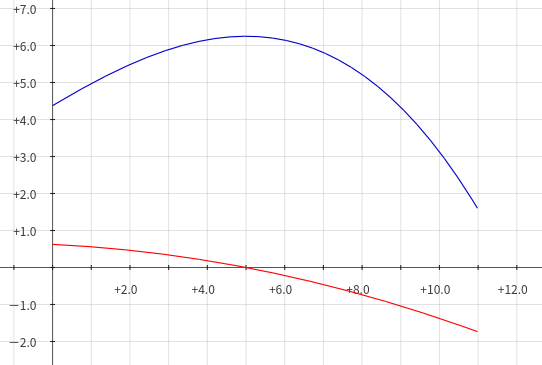
\includegraphics[scale=0.5]{images/wqs.png} % 插入图片
\end{center}

考虑原函数的导数的关系进行理解,令蓝色曲线为$g(x)$, 红色曲线为$g'(x)$。\par
设$C = 7$, 我们要求出$g(7)$, 因为$g(x)$是凸的,所以$g'(x)$是单调递减的,并且可以直接求出$g(x)$的最值,并且它是导函数与$x$轴的交点,发现$x = 5$的时候取到最值,但是它并不是我们想要的。\par
我们想要让导函数与$x$轴的交点移到$x = 7$的位置,这样直接求$g(x)$的最值就可以了。\par
令$f(x) = g(x) + kx$, $k$的现实意义是每多选一个物品,就要多付出$k$的代价, 并且发现$f'(x) = g'(x) + k$,那么$k$的函数意义就是让导函数向上平移了$k$个单位。\par
相当于导函数与$x$轴的交点右移,等价于$k$越大,交点也越向右,这样便是可二分的。\par
$k$的值域就是导函数的值域,根据求得的交点和$C$的大小关系,调整二分的方向。\par


\subsection{洛谷P2619}

题意:\par
给出一个无向带权连通图,每条边是黑色或白色, 求一棵最小权的恰好有$k$条边的生成树。\par

考虑不管$k$条边限制的最优值就是求最小生成树,那么带上权去二分即可。\par
直观的解释就是,如果白色的边多了,那么就增加选白色边的代价,这样在最小生成树中白色的边就会相应减少,反之亦然。

\begin{lstlisting}
#include <bits/stdc++.h>
using namespace std;
typedef long long ll;
const int N = 1e5 + 10;
const ll INF = 0x3f3f3f3f3f3f3f3f; 
int n, m, C; 

struct Edge { 
	int u, v, w, k, vis; 
	Edge() {}
	Edge(int u, int v, int w, int vis) : u(u), v(v), w(w), vis(vis) {k = 0;}
	bool operator < (const Edge &other) const {
		if (k + w == other.k + other.w) return vis > other.vis;
		return k + w < other.k + other.w;
	}
}e[N];

struct UFS {
	int fa[N];
	void init() { memset(fa, 0, sizeof fa); }
	int find(int x) { return fa[x] == 0 ? x : fa[x] = find(fa[x]); }
	bool merge(int u, int v) {
		int fu = find(u), fv = find(v);
		if (fu != fv) {
			fa[fu] = fv;
			return true;
		}
		return false;
	}
}ufs;

namespace WQS {
	int check(int K) {
		for (int i = 1; i <= m; ++i) {
			e[i].k = e[i].vis * K; 
		}
		sort(e + 1, e + 1 + m);
		ufs.init();
		int cnt_e = 0;  
		for (int i = 1; i <= m; ++i) {
			int u = e[i].u, v = e[i].v;
			if (ufs.merge(u, v)) cnt_e += e[i].vis;
		} 
		return cnt_e;
	}
	int calc(int K) {
		for (int i = 1; i <= m; ++i) {
			e[i].k = e[i].vis * K;
		}
		sort(e + 1, e + 1 + m);
		ufs.init();
		ll tot = 0; 
		for (int i = 1; i <= m; ++i) {
			int u = e[i].u, v = e[i].v, w = e[i].w;
			if (ufs.merge(u, v)) tot += w + e[i].k;
		}
		return tot - C * K;
	}
	void gao() {
		int l = -200, r = 100, res = -200;  
		while (r - l >= 0) {
		    int mid = (l + r) >> 1;	
			if (check(mid) >= C) {
				l = mid + 1;
				res = mid;
			} else {
				r = mid - 1;
			}
		}
		printf("%d\n", calc(res));
	}
}

int main() {
	while (scanf("%d%d%d", &n, &m, &C) != EOF) {
		for (int i = 1, u, v, w, vis; i <= m; ++i) {
			scanf("%d%d%d%d", &u, &v, &w, &vis);
			++u, ++v;
			e[i] = Edge(u, v, w, vis ^ 1);
		}
		WQS::gao();
	}
	return 0;
}
\end{lstlisting}

\subsection{Gym 101981B}

题意:\par

有$n$个人,他们所处的位置为$a_i(0 = a_1 < a_2 < \cdots < a_n \leq 10^9)$, 要恰好安排$k$个垃圾桶,令$D(a_i)$表示第$i$个人到离它最近的垃圾桶的距离,现在要安排$k$个垃圾桶的位置,使得$\sum\limits_{i = 1}^n D(a_i)$最少。

思路:\par

现在如果没有$k$这个限制,很好求,有这个限制套一个$WQS$二分即可。\par

再考虑怎么求$g(x)$的最值?\par
显然垃圾桶一定可以安排在某个人的位置,所以可选的位置只有$n$个。\par 

令$f_i$表示前$i$个位置的最短距离和,$g_i$表示当$i$放了一个垃圾桶,前$i$个位置的最短距离和,$S_i$表示$\sum\limits_{i = 1}^n a_i$。\par

我们考虑转移:

\begin{eqnarray*}
g_i &=& \min\limits_{j = 0}^{i - 1} f_j - (S_i - S_j) + (i - j) \cdot a_i \\
f_i &=& \min\limits_{j = 1}^{i - 1} g_j + (S_i - S_j) - (i - j) \cdot a_j
\end{eqnarray*}

考虑斜率优化,令$j > k$, 有:
\begin{eqnarray*}
\frac{(f_j + S_j) - (f_k + S_k)}{j - k} &\leq& a_i \\
\frac{(f_j - S_j + ja_j) - (f_k - S_k + ka_k)}{a_j - a_k} &\leq& i
\end{eqnarray*}

然后单调队列维护上凸包的斜率即可。\par

但是要注意这里还有一个垃圾桶个数的限制,这个转移的时候递推以下即可,并且我们发现当距离和相同的时候,垃圾桶个数越少越好,并且注意到$f_i, g_i$也有单调性,所以等价于维护斜率单调性的时候,如果存在$f_i = f_j(j > i)$的情况,是不会剔除$f_i$的,相当于维护斜率单调性的时候的等于号需要去掉。\par

这里$WQS$二分的时候的带的权可以考虑为每多加一个垃圾桶需要多付出的代价,如果当前放的垃圾桶比较少,那么我们就减少代价,否则增加代价。\par
上下界可以取为$[0, Sum[n] + 1]$即可。其实应该是$[-\infty, \infty]$,只是$[0, Sum[n] + 1]$和$[-\infty, \infty]$能达到的效果是一样的,即下界为$0$时,肯定是放$n$个垃圾桶距离和取到最小值,上界为$Sum[n] + 1$时,肯定是放$1$个垃圾桶距离和取到最大值。\par

时间复杂度$O(n \log n)$\par

\begin{lstlisting}
#include <bits/stdc++.h>
using namespace std;
using ll = long long;
using db = double;
using pLI = pair<ll, int>;
#define fi first
#define se second
const int N = 3e5 + 10;
const ll INF = 2e18;
int n, C, a[N]; ll S[N];

namespace WQS {
	//0 前i个位置的最值
	//1 前i个位置,并且第i个位置是集结点的最值
	struct frac {
		db x, y;
		frac(db x = 0, db y = 0) : x(x), y(y) { }
		bool operator < (const frac &other) const { return x * other.y < other.x * y; }
		bool operator > (const frac &other) const { return x * other.y > other.x * y; }
	};
	ll f[2][N]; db y[2][N], x[2][N]; int cnt[2][N];  
	int que[2][N], head[2], tail[2];
	frac slope(int k, int j, int id) { return frac(y[id][j] - y[id][k], x[id][j] - x[id][k]); }
	pLI check(ll k) {
		head[0] = 1; tail[0] = 0;
		head[1] = 1; tail[1] = 0; 
		que[0][++tail[0]] = 0;
		for (int i = 1, j; i <= n; ++i) {
			//第i个位置是集结点的最值
			while (head[0] < tail[0] && slope(que[0][head[0]], que[0][head[0] + 1], 0) < frac(a[i], 1)) ++head[0];
			j = que[0][head[0]];
			f[1][i] = f[0][j] - (S[i] - S[j]) + 1ll * (i - j) * a[i] + k;
			cnt[1][i] = cnt[0][j] + 1;
			y[1][i] = f[1][i] - S[i] + 1ll * i * a[i];
			x[1][i] = a[i];
			while (head[1] < tail[1] && slope(que[1][tail[1] - 1], que[1][tail[1]], 1) > slope(que[1][tail[1]], i, 1)) --tail[1];
			que[1][++tail[1]] = i;
			//前i个位置的最值
			while (head[1] < tail[1] && slope(que[1][head[1]], que[1][head[1] + 1], 1) < frac(i, 1)) ++head[1];
			j = que[1][head[1]];
			f[0][i] = f[1][j] + (S[i] - S[j]) - 1ll * (i - j) * a[j];
			cnt[0][i] = cnt[1][j];
			y[0][i] = f[0][i] + S[i];
			x[0][i] = i;
			while (head[0] < tail[0] && slope(que[0][tail[0] - 1], que[0][tail[0]], 0) > slope(que[0][tail[0]], i, 0)) --tail[0];
			que[0][++tail[0]] = i;
		}
		return pLI(f[0][n], cnt[0][n]); 
	}
	void gao() {
		ll l = 0, r = S[n] + 1, pos = 0;
		while (r - l >= 0) {
			ll mid = (l + r) >> 1;
			if (check(mid).se <= C) {
				r = mid - 1;
				pos = mid;	
			} else {
				l = mid + 1;
			}
		}
		printf("%lld\n", check(pos).fi - 1ll * pos * C);
	}
}

int main() {
	while (scanf("%d%d", &n, &C) != EOF) {
		S[0] = 0;
		for (int i = 1; i <= n; ++i) scanf("%d", a + i), S[i] = S[i - 1] + a[i];
		WQS::gao();	
	}
	return 0;
}
\end{lstlisting}

\section{高维前缀和}


子集:\par
$\forall i \in [0, 2^n - 1]$,求解$\sum\limits_{j \subset i} a_j$\par
\begin{lstlisting}
for(int j = 0; j < n; j++) 
    for(int i = 0; i < 1 << n; i++)
        if(i >> j & 1) f[i] += f[i ^ (1 << j)];
\end{lstlisting} \par

超集:\par
$\forall i \in [0, 2^n - 1]$,求解$\sum\limits_{i \subset j} a_j$\par
\begin{lstlisting}
for(int j = 0; j < n; j++) 
    for(int i = 0; i < 1 << n; i++)
        if(!(i >> j & 1)) f[i] += f[i ^ (1 << j)];
\end{lstlisting}

二维前缀和:\par
\begin{lstlisting}
for(int j = 0; j < n; j++) 
    for(int i = 0; i < 1 << n; i++)
        if(i >> j & 1) f[i] += f[i ^ (1 << j)];
\end{lstlisting} \par

三维前缀和:\par
\begin{lstlisting}
for(int i = 1; i <= n; i++)
    for(int j = 1; j <= n; j++)
        for(int k = 1; k <= n; k++) 
            a[i][j][k] += a[i - 1][j][k];
for(int i = 1; i <= n; i++)
    for(int j = 1; j <= n; j++)
        for(int k = 1; k <= n; k++)
            a[i][j][k] += a[i][j - 1][k];
for(int i = 1; i <= n; i++)
    for(int j = 1; j <= n; j++)
        for(int k = 1; k <= n; k++)
            a[i][j][k] += a[i][j][k - 1];
\end{lstlisting} \par

\subsection{ARC 100E}

题意:\par
给出$2^n$个数$a_i$,之后对于$\forall k \in [1, 2^n - 1]$,求出$a_i + a_j$的最大值,并且满足$i \; or \; j \leq k$\par
思路:\par
\begin{itemize}
\item 我们对于每个$k$都求出最大的$a_i + a_j$并且满足$i\; or \; j = k$,最后答案就是一个前缀最大值
\item 所以可以进一步转化为$i \; or \; j \subset k$,那么就将问题转化为了子集问题
\item 所以对于每个$k$,求出其所有子集的最大值和次大值即可
\end{itemize} \par
\begin{lstlisting}
#include <bits/stdc++.h>
using namespace std;
using pII = pair<int, int>;
#define fi first
#define se second
const int N = 1e6 + 10, INF = 0x3f3f3f3f;
int n, a[N], ans[N]; pII f[N];  
int main() {
	scanf("%d", &n);
	a[1 << n] = -INF;
	for (int i = 0; i < 1 << n; ++i) scanf("%d", a + i);
	for (int i = 0; i < 1 << n; ++i) f[i] = pII(i, 1 << n);
	for (int i = 0; i < n; ++i) {	
		for (int j = 0; j < 1 << n; ++j) {
			if ((j >> i) & 1) {
				int k = j ^ (1 << i);
				if (a[f[k].fi] > a[f[j].fi]) {
					f[j].se = f[j].fi;
					f[j].fi = f[k].fi;
				//	cout << j << " " << f[j].fi << " " << f[j].se << endl;
				} 
				if (f[k].fi != f[j].fi && a[f[k].fi] > a[f[j].se]) {
					f[j].se = f[k].fi;
				}
				if (f[k].se != f[j].fi && a[f[k].se] > a[f[j].se]) {
					f[j].se = f[k].se;
				} 
			//	cout << j << " " << f[j].fi << " " << f[j].se << endl;
			}
		}
	}
	memset(ans, 0, sizeof ans);
	for (int i = 1; i < 1 << n; ++i) {
		ans[i] = ans[i - 1];
	//	cout << i << " " << f[i].fi << " " << f[i].se << endl;
		if (f[i].fi != f[i].se && f[i].se != (1 << n)) {
			ans[i] = max(ans[i], a[f[i].fi] + a[f[i].se]);
		}
		printf("%d\n", ans[i]);
	}
	return 0;
}
\end{lstlisting}

\subsection{opentrains 010413F}


题意:\par
给出$n$个数,最多去掉$k$个数,使得剩下的数的$gcd$最大。\par
其中$k \leq \frac{n}{2}$\par

思路:\par

转化成至少保留$n - k$个数,使得$gcd$最大,因为$k \leq \frac{n}{2}$,故每个数属于最优解的概率至少为$\frac{1}{2}$,多随机几次,假设随机了$x$次,每次随机出来都不是
最优解的概率为$(\frac{1}{2})^x$,多随机几次,就能保证出答案。\par
然后枚举这个数的因数,看看剩下的数中出现的次数,大于等于$n - k - 1$就可以作为答案,可以大$gcd(a[i], k)$处统计答案,然后用高维前缀和统计出现次数。\par


\begin{lstlisting}
#include <bits/stdc++.h>
using namespace std;
using ll = long long;
const int N = 3e5 + 10;
int n, m, f[N];  
ll a[N], ans, fac[N], bk[N]; int tot;
vector <ll> vec;
mt19937 rd(time(0));
inline ll gcd(ll a, ll b) {
	return b ? gcd(b, a % b) : a;
}
inline ll mul(ll a, ll b, ll p) {
	return (a * b - (ll)(a / (long double)p * b + 1e-3) * p + p) % p;
}
inline ll qmod(ll base, ll n, ll p) {
	ll res = 1;
	base %= p;
	while (n) {
		if (n & 1) {
			res = mul(res, base, p);
		}
		base = mul(base, base, p);
		n >>= 1;
	}
	return res;
}

//此处需要Mill板子

inline int id(ll x) { return lower_bound(vec.begin(), vec.end(), x) - vec.begin(); }
void gao(ll x) {
	if (x == 1) return;
	mill.gao(x, vec);
	sort(fac + 1, fac + 1 + tot);
    tot = unique(fac + 1, fac + 1 + tot) - fac - 1;	
	memset(f, 0, sizeof f); 
	for (int i = 1; i <= n; ++i) {
		ll G = gcd(x, a[i]);
		++f[id(G)];
	}
	int sze = vec.size();
	for (int i = 1; i <= tot; ++i) {
		int j, k;
		for (j = k = sze - 1; j >= 0; --j) if (vec[j] % fac[i] == 0) {
			ll goal = vec[j] / fac[i];
			while (vec[k] > goal) --k;
			f[k] += f[j];
		}
	}
	for (int i = sze - 1; i >= 0; --i) {
		if (f[i] >= m) {
			ans = max(ans, vec[i]);
			break;
		}
	}
}

int main() {
	while (scanf("%d%d", &n, &m) != EOF) {
		m = n - m;
		for (int i = 1; i <= n; ++i)
			scanf("%lld", a + i);
		ans = 1;
		for (int i = 1; i <= 8; ++i) {
			int x = (rd() % n + n) % n + 1;
			gao(a[x]);
		}
		printf("%lld\n", ans); 
	}
	return 0;
}
\end{lstlisting}

\section{状压DP}
\subsection{带位置信息的状压}
CometOJ 52C\par
题意:\par
给出$n$张牌,一个合法的排列当且仅当编号为$i$的牌不在位置$p_i$上。\par
一个合法的排列的价值为:\par
\begin{eqnarray*}
\sum\limits_{i = 1}^n\sum\limits_{j = i + 1}^n [pos_j < pos_i] \cdot |j - i| \cdot |pos_i - pos_j|
\end{eqnarray*}
现在要求计算所有合法排列的价值和。\par
思路:\par
将贡献拆成$|j - i| \cdot pos_i$和$-|j - i| \cdot pos_j$\par
考虑$f[mask].fi$表示前$popcount(mask)$个位置已经放下了$mask$状态的牌的贡献和。\par
转移的时候枚举$mask$中一个已经存在的元素进行转移,并且钦定它放在$popcount(mask)$个位置,那么之前的元素都在它前面,还没放的元素都在它后面。\par
并且转移的时候需要维护一下方案数,时间复杂度$O(n^2 \cdot 2^n)$

\begin{lstlisting}
#include <bits/stdc++.h>
using namespace std;
using ll = long long;
using pLL = pair<ll, ll>;
#define fi first
#define se second
int n, p[20];
pLL f[(1 << 16) + 10];

int main() {
	int _T; cin >> _T;
	while (_T--) {
		scanf("%d", &n);
		for (int i = 1; i <= n; ++i) scanf("%d", p + i);
		memset(f, 0, sizeof f);
		f[0] = pLL(0, 1);
		for (int mask = 1; mask < (1 << n); ++mask) {
			int cnt = __builtin_popcount(mask);
			for (int i = 0; i < n; ++i) {
				if (((mask >> i) & 1) && p[i + 1] != cnt) {
					ll fee = 0;
					for (int j = 0; j < n; ++j) if (j != i) {
						if ((mask >> j) & 1) {
							if (i < j) fee += abs(i - j) * cnt;
						} else {
							if (i > j) fee -= abs(i - j) * cnt;
						}
					}
					int pre = mask ^ (1 << i);
					f[mask].se += f[pre].se;
					f[mask].fi += f[pre].fi + fee * f[pre].se;
				}
			}
		}
		printf("%lld\n", f[(1 << n) - 1].fi);
	}
	return 0;
}
\end{lstlisting}


\subsection{CometOJ 13D}

生成树装压$dp$。\par

题意:\par
有$n$个点,$m$条双向边$(u_i, v_i, w_i)$,表示连接了$u_i$和$v_i$,通过的时间为$w_i$。\par
令$d(i, j)$表示$i$到$j$的最短时间,定义一个道路系统的复杂度为$\sum\limits_{i = 1}^n \sum\limits_{j = 1}^n d(i, j)$。\par
删除一些道路,使得图连通的情况下,复杂度尽量高。\par
图中没有重边和自环,保证图连通, $1 \leq n \leq 14$。\par

思路:\par
最后的结果肯定是一棵生成树,因为边删的越多,复杂度越高。\par
考虑$f[S][i]$表示点集$S$是一棵子树,第$i$个点是根,转移的时候枚举以$j$为根,包含的点集为$T$,那么考虑可以从$f[i][S - T]$和$f[j][T]$转移过来,并且考虑$(i, j)$这条边产生的贡献。\par
考虑一条边$(i, j)$的转移,如果转移的贡献跟两边的子树大小有关,注意以$j$为根的子树是确定的,假设大小为$Size_j$,但是另一半的子树还没有确定,但是大小是知道的,是$n - Size_j$。\par

时间复杂度:$O(3^n \cdot n^2)$。\par

\begin{lstlisting}
#include <bits/stdc++.h>
#define SZ(x) ((int)x.size())
using namespace std;
typedef long long ll;
const ll INFLL = 0x3f3f3f3f3f3f3f3f;
const int N = 110;
int n, m;
int dist[20][20];
ll f[1 << 15][15];
vector <int> vec[1 << 15];

int main() {
	while (scanf("%d%d", &n, &m) != EOF) {
		memset(dist, -1, sizeof dist); 
		memset(f, -1, sizeof f);
	    for (int S = 0, len = (1 << n); S < len; ++S) {
			for (int i = 0; i < n; ++i) if ((S >> i) & 1)
				vec[S].push_back(i + 1); 
			if (SZ(vec[S]) == 1)
				f[S][*vec[S].begin()] = 0;
		}	
		for (int i = 1, u, v, w; i <= m; ++i) {
			scanf("%d%d%d", &u, &v, &w);
			dist[u][v] = dist[v][u] = w; 
		}
		ll res = 0;  
		for (int S = 1; S < (1 << n); ++S) { 
			for (auto &u : vec[S]) {
				// 枚举子集  
				for (int T = (S - 1) & S; T != 0; T = (T - 1) & S) {
					for (auto &v : vec[T]) {
						if (dist[u][v] == -1 || f[T][v] == -1 || f[S - T][u] == -1) continue;   
						f[S][u] = max(f[S][u], f[T][v] + f[S - T][u] + 1ll * dist[u][v] * SZ(vec[T]) * (n - SZ(vec[T])));  
					}
				}
				if (S == (1 << n) - 1)res = max(res, f[S][u]);
			}
		}
		printf("%lld\n", res);
	}
	return 0;
}
\end{lstlisting}

\section{数位DP}
2019Nowcoder多校第七场H. Pair\par

题意:\par
给出三个数$(A, B, C)$,问有多少对$(x, y)$满足:\par
\begin{itemize}
\item $1 \leq x \leq A$
\item $1 \leq y \leq B$
\item $x\;and\;y > C$ 或者 $x \; xor \; y < C$
\end{itemize} \par


思路:\par
考虑$f[i][j][k][l][m]$表示:
\begin{itemize}
\item 枚举到前$i$位
\item $x$是否卡到$A$的上界
\item $y$是否卡到$B$的上界
\item $x \; and \; y$是否已经大于$C$
\item $x \; and \; y$是否已经小于$C$
\end{itemize} \par
最后注意一下$0$的贡献,强行删去或者再加两位状态标记。\par

\begin{lstlisting}
#include <bits/stdc++.h>
using namespace std;
typedef long long ll;
#define N 100
 
ll A, B, C;
int a[N], b[N], c[N];
ll dp[N][3][3][2][2][2][2];
 
//位置 x&y x^y (=0 <1 >2)
ll DFS(int pos, int flag1, int flag2, int limit1, int limit2, int one1, int one2) {
    if (pos == -1 && (flag1 == 2 || flag2 == 1) && one1 == 1 && one2 == 1) {
        return 1ll;
    } else if (pos == -1) {
        return 0ll;
    }
    ll &res = dp[pos][flag1][flag2][limit1][limit2][one1][one2];
    if (res != -1) {
        return res;
    }
    res = 0;
    if (flag1 == 1 && flag2 == 2) {//x&y<C x^y>C 不合法
        return 0ll;
    }
    int l1 = limit1 ? a[pos] : 1;
    int l2 = limit2 ? b[pos] : 1;
    for (int i = 0; i <= l1; ++i) {
        for (int j = 0; j <= l2; ++j) {
            int x = i & j;
            int y = i ^j;
            int f1 = flag1;
            if (f1 == 0) {
                if (x > c[pos]) {
                    f1 = 2;
                } else if (x == c[pos]) {
                    f1 = 0;
                } else {
                    f1 = 1;
                }
            }
            int f2 = flag2;
            if (f2 == 0) {
                if (y > c[pos]) {
                    f2 = 2;
                } else if (y == c[pos]) {
                    f2 = 0;
                } else {
                    f2 = 1;
                }
            }
            res += DFS(pos - 1, f1, f2, limit1 && (i == a[pos]),
                       limit2 && (j == b[pos]), one1 | i, one2 | j);
        }
    }
    return res;
}
 
int main() {
    int T;
    scanf("%d", &T);
    while (T--) {
        scanf("%lld %lld %lld", &A, &B, &C);
        for (int i = 30; i >= 0; --i) {
            if (A & (1ll << i)) {
                a[i] = 1;
            } else {
                a[i] = 0;
            }
            if (B & (1ll << i)) {
                b[i] = 1;
            } else {
                b[i] = 0;
            }
            if (C & (1ll << i)) {
                c[i] = 1;
            } else {
                c[i] = 0;
            }
        }
        memset(dp, -1, sizeof dp);
        printf("%lld\n", DFS(30, 0, 0, 1, 1, 0, 0));
    }
    return 0;
}
\end{lstlisting}

\section{分治DP}

\subsection{二维分治}

CF 364E\par
题意:\par
给出一个$n \cdot m$的$01$矩形,找出有多少个子矩形满足其矩形和为$k$\par
$1 \leq n, m \leq 2500, 0 \leq k \leq 6$\par
思路:\par
考虑暴力就是枚举上下界再根据前缀和进行计数,复杂度是$O(n^2m)$\par
我们考虑分治能够改变统计的东西,我们考虑横向切一刀,统计跨过$mid$的合法区间个数,那么我们统计一下$up_{0, k}$表示从$mid$往上走矩形和$\geq k$的第一个位置,$up_{1, k}$表示$mid + 1$往下走矩形和$\geq k$的第一个位置,这个随着另一维度区间长度的缩小具有单调性,那么最后答案就是
\begin{eqnarray*}
\sum\limits_{i = 0}^K (up[0][i] - up[0][i + 1]) * (up[1][K - k + 1] - up[1][K - k])
\end{eqnarray*} \par
注意要判断一下$up_{0, k}$和$up_{1, K - k}$这两个位置是否是矩形和恰好等于$k$和$K - k$的。\par
时间复杂度$O(n^2klogn)$

\begin{lstlisting}
#include <bits/stdc++.h>
using namespace std;
using ll = long long;
const int N = 3e3 + 10;
int n, m, K, a[N][N], S[N][N], up[2][10]; 
ll res;

inline int get(int x1, int x2, int y1, int y2) {
	if (x1 > x2 || y1 > y2) return 0;
	x1 = max(x1, 1); y1 = max(y1, 1);
	return S[x2][y2] - S[x1 - 1][y2] - S[x2][y1 - 1] + S[x1 - 1][y1 - 1];
}

void gao(int x1, int x2, int y1, int y2) {
	if (x1 > x2 || y1 > y2) return;
	if (x1 == x2 && y1 == y2) {
		res += a[x1][y1] == K;
		return;
	}
	if (x2 - x1 > y2 - y1) {
		int mid = (x1 + x2) >> 1;
		gao(x1, mid, y1, y2);
		gao(mid + 1, x2, y1, y2);
		for (int i = y1; i <= y2; ++i) {
			for (int k = 0; k <= K + 1; ++k) up[0][k] = mid, up[1][k] = mid + 1;
			for (int j = y2; j >= i; --j) {
				for (int k = 0; k <= K + 1; ++k) {
					while (up[0][k] >= x1 && get(up[0][k], mid, i, j) < k) --up[0][k];
					while (up[1][k] <= x2 && get(mid + 1, up[1][k], i, j) < k) ++up[1][k];	
				}
				for (int k = 0; k <= K; ++k) {
					if (get(up[0][k], mid, i, j) == k && get(mid + 1, up[1][K - k], i, j) == K - k) {
						res += 1ll * (up[0][k] - up[0][k + 1]) * (up[1][K - k + 1] - up[1][K - k]);
					}
				}
			}
		}
	} else {
		int mid = (y1 + y2) >> 1;
		gao(x1, x2, y1, mid);
		gao(x1, x2, mid + 1, y2);
		for (int i = x1; i <= x2; ++i) {
			for (int k = 0; k <= K + 1; ++k) up[0][k] = mid, up[1][k] = mid + 1;
		   	for (int j = x2; j >= i; --j) {
				for (int k = 0; k <= K + 1; ++k) {
					while (up[0][k] >= y1 && get(i, j, up[0][k], mid) < k) --up[0][k];
					while (up[1][k] <= y2 && get(i, j, mid + 1, up[1][k]) < k) ++up[1][k];
				}
				for (int k = 0; k <= K; ++k) {
					if (get(i, j, up[0][k], mid) == k && get(i, j, mid + 1, up[1][K - k]) == K - k) {
						res += 1ll * (up[0][k] - up[0][k + 1]) * (up[1][K - k + 1] - up[1][K - k]);
					}
				}
		   	}	
		}
	}
}

int main() {
	scanf("%d%d%d", &n, &m, &K);
	for (int i = 1; i <= n; ++i) {
		static char s[N]; scanf("%s", s);
		for (int j = 0; j < m; ++j) {
			a[i][j + 1] = s[j] - '0';
			S[i][j + 1] = S[i - 1][j + 1] + S[i][j] - S[i - 1][j] + a[i][j + 1];
		}
	}
	res = 0;
	gao(1, n, 1, m);
	printf("%lld\n", res);
	return 0;
}
\end{lstlisting}


\section{基础知识}

弧度制和角度制:$\displaystyle 1rad = \frac{180}{\pi} \approx 57.3\degree\;\;\; 1\degree = \frac{\pi}{180} \approx 0.01745rad$\par

包围凸包的圆角多边形: 弄一个圆角多边形包围凸包,并且使得凸包上的每个点到圆角多边形的距离为$d$,那么该圆角多边形的周长为凸包的周长$+$半径为$d$的圆的周长\par

阿波罗尼斯圆:\par

\begin{figure}[ht]
\centering  %居中显示
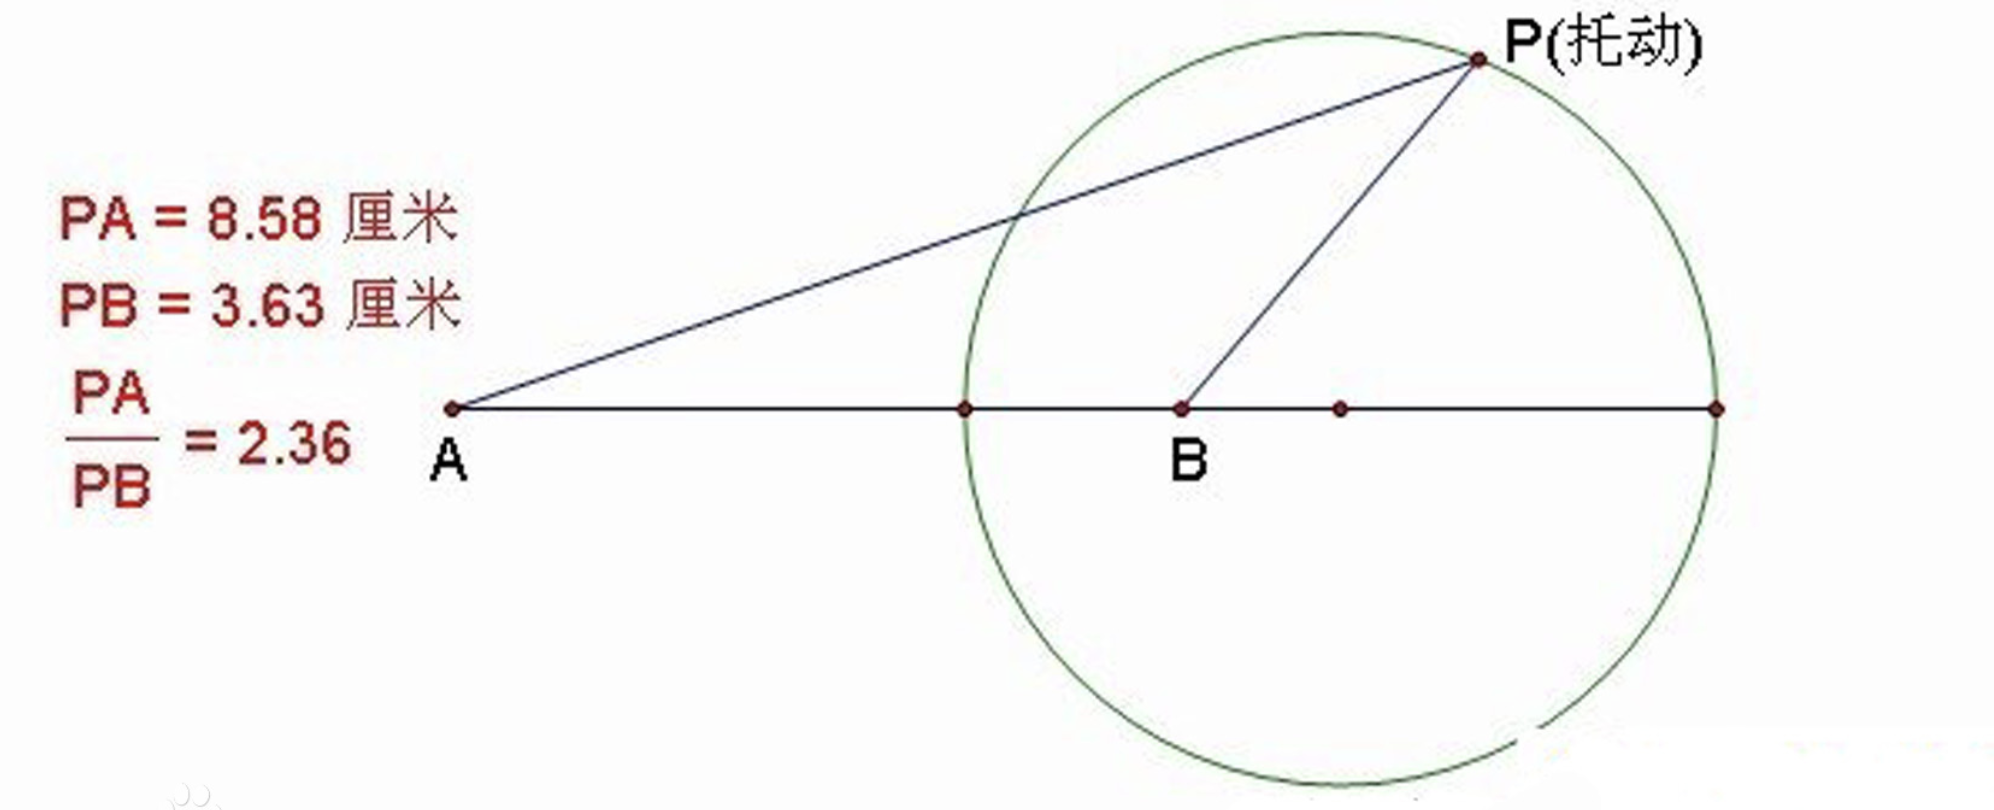
\includegraphics[scale=0.35]{images/Apollonius_circle.png} % 插入图片
\end{figure}

令$B$为坐标原点, $A$的坐标为$(a, 0)$, 则动点$P(x, y)$满足$\displaystyle \frac{PA}{PB} = k(k > 0 \mbox{且} k \neq 1)$\par
且$\displaystyle PA = \sqrt{(x - a)^2 + y^2}$, $\displaystyle PB = \sqrt{x^2 + y^2}$\par
整理得:$\displaystyle (k^2 - 1)(x^2 + y^2) + 2ax - a^2 = 0$\par
\begin{itemize}
\item 当$k > 0 \mbox{且} k \neq 1$时, 它是圆
\item 当$k = 1$时, 轨迹是两点连线的中垂线
\end{itemize}

球缺:\par
用一个平面截去一个球所得部分叫球缺。\par
球缺面积:$\displaystyle 2\pi h$。\par
球缺体积:$\displaystyle \pi \cdot h^2 \cdot (R - \frac{h}{3})$\par
球缺质心:匀质球缺的质心位于它的中轴线上,并且与底面的距离为$\displaystyle C = \frac{(4\cdot R - h) \cdot h}{12 \cdot R - 4 \cdot h} = \frac{(d^2 + 2\cdot h^2) \cdot h}{3\cdot d^2 + 4\cdot h^2}$\par
其中,$h$为球缺的高,$R$为大圆半径,$d$为球缺的底面直径。\par

\section{皮克定理}
给定顶点坐标均是整点(或正方形格子点)的简单多边形,皮克定理说明了其面积$S$和内部格点数目$i$、边上格点数目$b$的关系:
\begin{eqnarray*}
S = i + \frac{b}{2} - 1
\end{eqnarray*}

\section{欧拉公式}
\begin{eqnarray*}
V - E + F = 2
\end{eqnarray*}\par
其中$V$是顶点, $E$是边, $F$是面。\par
适用于所有多边形,无论维度。\par

\section{婆罗摩笈多公式}
\begin{center}
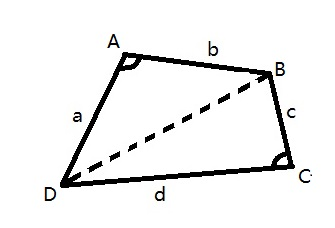
\includegraphics[scale=0.65]{images/Snipaste_2019-09-28_15-09-51.png} % 插入图片
\end{center}
已知四边形四边长$a, b, c, d$,那么其面积为:
\begin{eqnarray*}
S = \sqrt{(p - a)(p - b)(p - c)(p - d) - abcdcos^2\theta}
\end{eqnarray*}\par
其中$p = \frac{a + b + c + d}{2}$。

\section{点积}
对于向量$a$和向量$b$,有:
\begin{eqnarray*}
	a &=& [a_1, a_2, \cdots, a_n] \\
	b &=& [b_1, b_2, \cdots, b_n]
\end{eqnarray*} \par
$a$和$b$的点积公式为:
\begin{eqnarray*}
	a \cdot b = a_1b_1 + a_2b_2 + \cdots + a_nb_n
\end{eqnarray*} \par

\textbf{几何意义}\par
点积的几何意义用来表示或计算两个向量之间的夹角,以及向量$b$在向量$a$上的投影:
\begin{eqnarray*}
	a \cdot b = |a| \cdot |b|\cos\theta
\end{eqnarray*} \par

其含义为向量$a$在$b$上的投影长度和$|b|$的乘积。\par

点积和两向量之间的夹角关系:\par
$a \cdot b > 0$,夹角范围:$[0^\circ, 90^\circ)$ \par
$a \cdot b = 0$,两向量垂直 \par
$a \cdot b < 0$,夹角范围:$(90^\circ, 180^\circ]$ \par

\section{叉积}
我们令$\overrightarrow{A} = (x_1, y_1, z_1), \overrightarrow{B} = (x_2, y_2, z_2)$,那么有:\par
\begin{eqnarray*}
\overrightarrow{A} \times \overrightarrow{B} = 
\left|
\begin{array} {cccc}
 i &    j    & k \\ 
 x_1 &  y_1   & z_1\\ 
 x_2 & y_2 & z_2 
\end{array}
\right| 
= 
\left|
\begin{array}{cccc}
y_1 & z_1 \\
y_2 & z_2 \\
\end{array}
\right|i
- 
\left|
\begin{array}{cccc}
x_1 & z_1 \\
x_2 & z_2 
\end{array}
\right|j
+ 
\left|
\begin{array}{cccc}
x_1 & y_1 \\
x_2 & y_2
\end{array}
\right|k
= (y_1z_2 - z_1y_2)i - (x_1z_2 - z_1x_2)j + (x_1y_2 - y_1x_2)k 
\end{eqnarray*}

\subsection{代数性质}
对于任意三个向量$\overrightarrow{A}$、$\overrightarrow{B}$、$\overrightarrow{C}$、$\overrightarrow{D}$有:
\begin{itemize}
\item $\overrightarrow{A} \times \overrightarrow{A} = \overrightarrow{0}$
\item $\overrightarrow{A} \times \overrightarrow{0} = \overrightarrow{0}$
\item $\overrightarrow{A} \times \overrightarrow{B} = -(\overrightarrow{B} \times \overrightarrow{A})$ (反交换律)
\item $\overrightarrow{A} \times (\overrightarrow{B} + \overrightarrow{C}) = \overrightarrow{A} \times \overrightarrow{B} + \overrightarrow{A} \times \overrightarrow{C}$,(加法的左分配律)
\item $(\overrightarrow{A} + \overrightarrow{B}) \times \overrightarrow{C} = \overrightarrow{A} \times \overrightarrow{C} + \overrightarrow{B} \times \overrightarrow{C}$,(加法的右分配律)
\item $(\lambda\overrightarrow{A}) \times \overrightarrow{B} = \lambda(\overrightarrow{A} \times \overrightarrow{B}) = \overrightarrow{A} \times (\lambda\overrightarrow{B})$
\item $\overrightarrow{A} \times \overrightarrow{B} + \overrightarrow{C} \times \overrightarrow{D} = (\overrightarrow{A} - \overrightarrow{C}) \times (\overrightarrow{B} - \overrightarrow{D}) + \overrightarrow{A} \times \overrightarrow{D} + \overrightarrow{C} \times \overrightarrow{B}$
\item 
\begin{eqnarray*}
\left|
\begin{array}{cccc}
\overrightarrow{A} \times \overrightarrow{B}
\end{array}
\right|
=
\left|
\begin{array}{cccc}
\overrightarrow{B} \times \overrightarrow{A}
\end{array}
\right|
\end{eqnarray*}
\item
\begin{eqnarray*}
\left|
\begin{array}{cccc}
\overrightarrow{A} \times \overrightarrow{B}
\end{array}
\right|^2 
=
|\overrightarrow{A}|^2|\overrightarrow{B}|^2 - (\overrightarrow{A} \cdot \overrightarrow{B})^2
=
\left|
\begin{array}{cccc}
\overrightarrow{A} \cdot \overrightarrow{A} \;&\; \overrightarrow{A} \cdot \overrightarrow{B} \\
\overrightarrow{A} \cdot \overrightarrow{B} \;&\; \overrightarrow{B} \cdot \overrightarrow{B}
\end{array}
\right|
\end{eqnarray*} 
\centerline{(拉格朗日恒等式)}
\end{itemize}

\subsection{二维向量叉积}
我们令$\overrightarrow{A} = (x_1, y_1, 0), \overrightarrow{B} = (x_2, y_2, 0)$,那么有:
\begin{eqnarray*}
\overrightarrow{A} \times \overrightarrow{B} 
= 
(x_1y_2 - y_1x_2)k
\end{eqnarray*} \par
那么向量的模:
\begin{eqnarray*}
|\overrightarrow{A} \times \overrightarrow{B}| = |\overrightarrow{A}||\overrightarrow{B}|\sin\theta = (x_1y_2 - x_2y_1)
\end{eqnarray*} \par
其意义为两向量构成的平行四边形的有向面积。
\subsection{二维向量叉积的几何意义}
\begin{itemize}
\item $\overrightarrow{A} \times \overrightarrow{B} < 0$时,$\overrightarrow{B}$对应的向量在$\overrightarrow{A}$的顺时针方向(右边)。
\item $\overrightarrow{A} \times \overrightarrow{B} = 0$时,$\overrightarrow{A}$、$\overrightarrow{B}$共线。
\item $\overrightarrow{A} \times \overrightarrow{B} > 0$时,$\overrightarrow{B}$在$\overrightarrow{A}$的逆时针方向(左边)。
\end{itemize}

\section{直线}
\begin{enumerate}
\item 一般式 
\begin{eqnarray*}
Ax + By + C = 0
\end{eqnarray*} \par
一般式说明了平面直角坐标系上一个一元二次方程表示一条直线。\par
斜率:$k = -\frac{A}{B}$。\par
法向量:$\overrightarrow{n} = (A, B)$。\par
方向向量:$\overrightarrow{a} = (B, -A)$。\par
$x$轴上的截距:$-\frac{C}{A}$,$y$轴上的截距:$-\frac{C}{B}$。

\item 点斜式 
\begin{eqnarray*}
y - y_0 = k(x - x_0)
\end{eqnarray*} \par
点斜式是由一个定点$P(x_0, y_0)$和斜率$k$确定的直线方程。\par
斜率:$k$。\par
法向量:$\overrightarrow{n} = (k, -1)$。\par
方向向量:$\overrightarrow{a} = (1, k)$。\par
$x$轴上的截距为:$-\frac{y_0}{k} + x_0$,$y$轴上的截距为:$y_0 - kx_0$。

\item 斜截式 
\begin{eqnarray*}
y = kx + b
\end{eqnarray*} \par
斜截式是由斜率$k$和$y$轴上的截距$b$确定的直线方程。\par
斜率:$k$。\par
法向量:$\overrightarrow{n} = (k, -1)$。\par
方向向量:$\overrightarrow{a} = (1, k)$。\par
$x$轴上的截距为:$-\frac{b}{k}$,$y$轴上的截距为:$-b$。

\item 两点式 
\begin{eqnarray*}
\frac{y - y_1}{y_2 - y_1} = \frac{x - x_1}{x_2 - x_1}
\end{eqnarray*} \par
两点式是由已知的两个点$(x_1,y_1)$、$(x_2,y_2)$所确定的直线方程。\par
斜率:$k = \frac{y_2 - y_1}{x_2 - x_1}$\par
法向量:$\overrightarrow{n} = (y_2 - y_1, x_1 - x_2)$\par
方向向量:$\overrightarrow{a} = (x_2 - x_1, y_2 - y_1)$\par
$x$轴上的截距:$\frac{x_1y_2 - x_2y_1}{y_2 - y_1}$,$y$轴上的截距:$\frac{x_2y_1 - x_1y_2}{x_2 - x_1}$\par
通过变形有:
\begin{eqnarray*}
\frac{y - y_1}{y_2 - y_1} = \frac{x - x_1}{x_2 - x_1} 
\end{eqnarray*} \par
等价于:
\begin{eqnarray*}
(y - y_1)(x_2 - x_1) = (x - x_1)(y_2 - y_1)
\end{eqnarray*} \par
有:
\begin{eqnarray*}
(y_2 - y_1)x - (x_2 - x_1)y = y_1x_2 - y_2x_1
\end{eqnarray*}\par
令:
\begin{eqnarray*}
a &=& y_2 - y_1 \\
b &=& x_2 - x_1 \\
c &=& y_1x_2 - y_2x_1
\end{eqnarray*} \par
这样就可以写成$ax - by = c$的形式,并且当给出的两点均为整数时,$a, b, c$均为整数。

\item 点向式 
\begin{eqnarray*}
\frac{y - y_0}{b} = \frac{x - x_0}{a}
\end{eqnarray*} \par
点向式是由已知的定点$P(x_0,y_0)$和方向向量$\overrightarrow{\textbf{a}}=(a,b)$所确定的直线方程。\par
斜率:$k = \frac{b}{a}$\par
法向量:$\overrightarrow{n} = (b, -a)$\par
方向向量:$\overrightarrow{a} = (a, b)$\par
$x$轴上的截距为:$\frac{x_1y_2-x_2y_1}{y_2-y_1}$,$y$轴上的截距为:$\frac{x_1y_1-x_1y_2}{x_2-x_1}$\par

\item 参数式
\begin{eqnarray*}
\left\{
\begin{array}{cccc}
&x=x_0+at  & \\ 
&y = y_0+bt  & \\
\end{array}
\right.
\end{eqnarray*}\par
这里的参数是$t$,是点向式的变式,也是由定点$P(x_0,y_0)$和方向向量$\overrightarrow{\textbf{a}}=(a,b)$确定的。\par
斜率:$k = \frac{b}{a}$\par
法向量:$\overrightarrow{\textbf{n}}=(b,-a)$\par
方向向量:$\overrightarrow{\textbf{a}}=(a,b)$\par
$x$轴上的截距为:$x_0-\frac{a}{b}y_0$,$y$轴上的截距为:$y_0-\frac{b}{a}x_0$\par

\item 特别参数式
\begin{eqnarray*}
\left\{
\begin{array}{cccc}
&x=x_0+tcos\alpha   & \\ 
&y = y_0+tsin\alpha   & \\
\end{array}
\right.
\end{eqnarray*}\par
这里的参数是$t$,是参数式的特例,即以直线的倾角$\alpha$为参数。
斜率:$tan\alpha$ \par
法向量:$\overrightarrow{\textbf{n}}=(sin\alpha ,-cos\alpha )$\par
方向向量:$\overrightarrow{\textbf{a}}=(cos\alpha ,sin\alpha )$\par
x轴上的截距为:$x_0-\frac{1}{tan\alpha }y_0$,$y$轴上的截距为:$y_0-tan\alpha x_0$\par

\item 点法式
\begin{eqnarray*}
A(x-x_0)+B(y-y_0)=0
\end{eqnarray*}\par
点法式是由定点$P(x_0,y_0)$和方向量$\overrightarrow{\textbf{n}}=(A ,B)$直接确定的直线方程。\par
斜率:$-\frac{A}{B}$\par
法向量:$\overrightarrow{\textbf{n}}=(A ,B)$\par
方向向量:$\overrightarrow{\textbf{a}}=(B ,-A )$\par
x轴上的截距为:$x_0+\frac{B}{A}y_0$,$y$轴上的截距为:$y_0+\frac{A}{B} x_0$

\item 截距式
\begin{eqnarray*}
\frac{x}{a} + \frac{y}{b} = 1
\end{eqnarray*}\par
截距式是由$x$轴上的截距$a$和$y$轴上的截距$b$直接确定的直线方程,当然必须要截距不为$0$。\par
斜率:$k = - \frac{b}{a}$\par
法向量:$\overrightarrow{\textbf{n}}=(\frac{1}{a},\frac{1}{b})$\par
方向向量:$\overrightarrow{\textbf{a}}=(a,-b)$\par
$x$轴上的截距为:$a$,$y$轴上的截距为:$b$\par

\item 点法式
\begin{eqnarray*}
xcos\theta + ysin\theta -p=0
\end{eqnarray*}\par
点法式是由直线与$y$轴的夹角$\theta$与原点$O$到直线的距离$p$,这里$p>0$,$\theta$是直线逆时针转向$y$轴的夹角。\par
斜率:$k = -tan\theta$\par 
法向量:$\overrightarrow{\textbf{n}}=(cos\theta ,sin\theta )$\par
方向向量:$\overrightarrow{\textbf{a}}=(sin\theta ,-cos\theta )$\par
$x$轴上的截距为:$\frac{p}{cos\theta }$,$y$轴上的截距为:$\frac{p}{sin\theta }$\par

\item 切线式
\begin{eqnarray*}
x_0x+y_0y=r^2
\end{eqnarray*} \par
切线式表达的几何意义是,以原点$O$为圆心,$r$为半径,$P(x_0,y_0)$为切点的圆的切线。\par
斜率:$k = -\displaystyle{\frac{x_0}{y_0}}$\par
法向量:$\overrightarrow{\textbf{n}}=(x_0 ,y_0)$\par
方向向量:$\overrightarrow{\textbf{a}}=(y_0 ,-x_0 )$\par
$x$轴上的截距为:$\displaystyle{\frac{r^2}{y_0 }}$,$y$轴上的截距为:$\displaystyle{\frac{r^2}{x_0}}$\par

\item 直线与直线的位置关系\par
设有两条直线$l_1$、$l_2$,斜率分别为$k_1$、$k_2$,法向量分别为$\overrightarrow{n_1}$、$\overrightarrow{n_2}$,放量向量分别为$\overrightarrow{a_1}$、$\overrightarrow{a_2}$,那么则有:\par
两直线平行的判定:$l_1//l_2\Leftrightarrow k_1=k_2\Leftrightarrow \overrightarrow{n_1}//\overrightarrow{n_2}\Leftrightarrow \overrightarrow{a_1}//\overrightarrow{a_2}$\par
两直线垂直的判定:$l_1\bot l_2\Leftrightarrow k_1\cdot k_2=-1\Leftrightarrow \overrightarrow{n_1}\bot \overrightarrow{n_2}\Leftrightarrow \overrightarrow{a_1}\bot \overrightarrow{a_2}$\par
两直线的夹角$\theta$ :$cos\theta =|\frac{k_1-k_2}{1+k_1k_2}| =|\frac{\overrightarrow{n_2}\cdot \overrightarrow{n_1}}{|\overrightarrow{n_1}|\cdot |\overrightarrow{n_2}|}| =|\frac{\overrightarrow{a_2}\cdot \overrightarrow{a_1}}{|\overrightarrow{a_1}|\cdot |\overrightarrow{a_2}|}| $\par
直线上两点间距离$d$(主要用于求解弦长):$d=\sqrt{1+k^2} |x_2-x_1|=\sqrt{1+k^2} |y_2-y_1|= |t_2-t_1|$,这里的$t$就是参数方程中的$t$,$t$的几何意义便是直线上动点$(x,y)$到定点$(x_0,y_0)$的有向线段的数量。\par

\textbf{总结}:直线的斜率表达了直线与x轴的夹角,法向量是垂直于直线的向量,方向向量是平行于直线的向量,因此可以用斜率、法向量、方向向量来判断平行、垂直与夹角。\par


\end{enumerate}


\section{三角形相关}

\subsection{面积}

\begin{itemize}
\item 叉积
\begin{eqnarray*}
\frac{1}{2} \overrightarrow{AB} \times \overrightarrow{AC}
\end{eqnarray*} 

\item 海伦公式
\begin{eqnarray*}
S = \sqrt{p(p-a)(p-b)(p-c)},\;\;\;p=\frac{a+b+c}{2}
\end{eqnarray*} 

\item 
\begin{eqnarray*}
S = \frac{absinC}{2}
\end{eqnarray*}
\end{itemize}

\subsection{费马点}
该点到三角形三个顶点的距离之和最小。\par
如果三角形有一个内角大于或等于$120\degree$,这个内角的顶点就是费马点;如果$3$个内角均小于$120\degree$,则在三角形内部对$3$边张角均为$120\degree$的点,是三角形的费马点。\par
设三角形三条边为$a, b, c$, 且不妨假设$a \leq b \leq c$,那么费马点到三点的距离和为: 
\begin{itemize}
\item 有一个内角大于$120\degree$, 距离为$a + b$
\item 三个内角均小于$120\degree$, 距离为$\displaystyle \sqrt{\frac{a^2 + b^2 + c^2 + 4\sqrt{3} \cdot s}{2}}$
\end{itemize}


\subsection{外心}
三边中垂线交点,到三角形三个顶点距离相同, 外接圆圆心。

\subsection{内心}
角平分线的交点,到三角形三边的距离相同, 内切圆圆心。


\subsection{垂心}
三条高线的交点。

\subsection{重心}
三条中线的交点,到三角形三顶点距离的平方和最小的点,三角形内到三边距离之积最大的点


\section{欧拉四面体公式}
HDU 1411\par

\begin{eqnarray*}
V^2 = \frac{1}{36}
\left|
\begin{array}{cccc}
p^2 & \frac{p^2 + q^2 - n^2}{2} & \frac{p^2 + r^2 - m^2}{2} \\
\frac{p^2 + q^2 - n^2}{2} & q^2 & \frac{q^2 + r^2 - l^2}{2} \\
\frac{p^2 + r^2 - m^2}{2} & \frac{q^2 + r^2 - l^2}{2} & r^2
\end{array}
\right|
\end{eqnarray*}

\begin{lstlisting}
#include <bits/stdc++.h>
using namespace std;
using db = double;

// 求四面体的体积,欧拉公式
// p, q, r 为AB,AC,AD, n, m, l 为BC, BD, CD
db V(db p, db q, db r, db n, db m, db l) {
    db rr = r * r, mm = m * m, nn = n * n;
    db pp = p * p, qq = q * q, ll = l * l;
    db x1 = (pp + qq - nn) / 2.0, x2 = (pp + rr - mm) / 2.0, x3 = (qq + rr - ll) / 2.0;
    db v = pp * (qq * rr - x3 * x3) - x1 * (x1  * rr - x2 * x3) + x2 * (x1 * x3 - qq * x2);
    return sqrt(v) / 6.0;
}

int main() {
	db p, q, r, n, m, l;
	while (cin >> p >> q >> r >> n >> m >> l) {
		printf("%.4lf\n", V(p, q, r, n, m, l));
	}
	return 0;
}
\end{lstlisting}

\section{一切的开始}

\begin{lstlisting}
typedef double db;
const db eps = 1e-10;
const db PI = acos(-1.0L); 
//long long类型时使用
//int sgn(db x) { if (x == 0) return 0; return x < 0 ? -1 : 1; }
int sgn(db x) { if (fabs(x) < eps) return 0; return x < 0 ? -1 : 1; }
db sqr(db x) { return x * x; }
db fixOut(db x) { if (sgn(x) == 0) return 0; return x; }
db toRad(db angle) { return angle / 180 * PI; }
\end{lstlisting}

\section{二维几何}


\subsection{点、线}
\begin{lstlisting}
struct Point {
	db x, y;
	Point(db x = 0, db y = 0) : x(x), y(y) {}
	void scan() { db _x, _y; scanf("%lf%lf", &_x, &_y); x = _x, y = _y; }
	void print() { printf("%.11f %.11f\n", x, y); }
	bool operator == (const Point &b) const { return sgn(x - b.x) == 0 && sgn(y - b.y) == 0; }
	bool operator < (const Point &b) const { return sgn(x - b.x) == 0 ? sgn(y - b.y) < 0 : x < b.x; }
	Point operator + (const Point &b) const { return Point(x + b.x, y + b.y); }
	Point operator - (const Point &b) const { return Point(x - b.x, y - b.y); }
	Point operator * (const db &b) const { return Point(x * b, y * b); }
	Point operator / (const db &b) const { return Point(x / b, y / b); }
	db operator ^ (const Point &b) const { return x * b.y - y * b.x; }
	db operator * (const Point &b) const { return x * b.x + y * b.y; }
	db len() { return hypot(x, y); }
	db len2() { return x * x + y * y; }
	db dis(Point b) { return hypot(x - b.x, y - b.y); }
	db dis2(Point b) { return (x - b.x) * (x - b.x) + (y - b.y) * (y - b.y); }
	int quad() {
		int _x = sgn(x), _y = sgn(y);
		if (_x > 0 && _y >= 0) return 1;
		if (_x <= 0 && _y > 0) return 2;
		if (_x < 0 && _y <= 0) return 3;
		if (_x >= 0 && _y < 0) return 4;
	}
	//求PA和PB构成的夹角 lightOJ 1203
	db getRad(Point a, Point b) {
		Point p = *this;
		return fabs(atan2(fabs((a - p) ^ (b - p)), (a - p) * (b - p)));
	}
	//单位法向量
	Point normal() { return Point(-y, x) / len(); }
	//化为长度为r的向量
	Point trunc(db r) {
		db l = len();
		if (!sgn(l)) return *this;
		r /= l;
		return Point(x * r, y * r);
	}
	//逆时针旋转90度
	Point rotleft() { return Point(-y, x); }
	//顺时针旋转90度
	Point rotright() { return Point(y, -x); }
	//绕点p旋转rad弧度
	Point rotate(Point p, db rad) {
		Point v = (*this) - p;
		db c = cos(rad), s = sin(rad);
		return Point(p.x + v.x * c - v.y * s, p.y + v.x * s + v.y * c);
	}
};

struct Line {
	Point s, e;
	Line() {}
	Line(Point s, Point e) : s(s), e(e) {}
	void scan() { s.scan(); e.scan(); }
	void print() { s.print(); e.print(); }
	bool operator == (const Line &b) const { return s == b.s && e == b.e; }
	//根据一个点和倾斜角确定直线,0 <= angle <= PI
	Line(Point p, db rad) {
		s = p;
		if (sgn(rad - PI / 2) == 0) {
			e = (s + Point(0, 1));
		} else {
			e = (s + Point(1, tan(rad)));
		}
	}
	//ax + by + c = 0
	Line(db a, db b, db c) {
		if (sgn(a) == 0) {
			s = Point(0, -c / b);
			e = Point(1, -c / b);
		} else if (sgn(b) == 0) {
			s = Point(-c / a, 0);
			e = Point(-c / a, 1);
		} else {
			s = Point(0, -c / b);
			e = Point(1, (-c - a) / b);
		}
	}
	void adjust() { if (e < s) swap(s, e); }
	db length() { return s.dis(e); }
	//返回直线倾斜角 0 <= rad <= PI
	db getAngle() {
		db k = atan2(e.y - s.y, e.x - s.x);
		if (sgn(k) < 0) k += PI;
		if (sgn(k - PI) == 0) k -= PI;
		return k;
	}
	//点和直线关系
	//1 在左侧
	//2 在右侧
	//3 在直线上
	int relationPoint(Point p) {
		int c = sgn((p - s) ^ (e - s));
		if (c < 0) return 1;
		if (c > 0) return 2;	
		return 3;
	}
	//判断点是否在线段上
	bool pointOnSeg(Point p) { return sgn((p - s) ^ (e - s)) == 0 && sgn((p - s) * (p - e)) <= 0; }
	//判断两向量是否平行
	bool parallel(Line b) { return sgn((e - s) ^ (b.e - b.s)) == 0; }
	//两线段相交判断
	//2 规范相交
	//1 非规范相交
	//0 不相交
	int segCrossSeg(Line b) {
		int d1 = sgn((e - s) ^ (b.s - s));
		int d2 = sgn((e - s) ^ (b.e - s));
		int d3 = sgn((b.e - b.s) ^ (s - b.s));
		int d4 = sgn((b.e - b.s) ^ (e - b.s));
		if ((d1 ^ d2) == -2 && (d3 ^ d4) == -2) return 2;
		return ((d1 == 0 && sgn((b.s - s) * (b.s - e)) <= 0) ||
				(d2 == 0 && sgn((b.e - s) * (b.e - e)) <= 0) ||
				(d3 == 0 && sgn((s - b.s) * (s - b.e)) <= 0) ||
				(d4 == 0 && sgn((e - b.s) * (e - b.e)) <= 0));
	}
	//直线和线段相交判断
	//2 规范相交
	//1 非规范相交
	//0 不相交
	int lineCrossSeg(Line b) {
		int d1 = sgn((e - s) ^ (b.s - s));
		int d2 = sgn((e - s) ^ (b.e - s));
		if ((d1 ^ d2) == -2) return 2;
		return (d1 == 0 || d2 == 0);
	}
	//两直线关系
	//0 平行
	//1 重合
	//2 相交
	int lineCrossLine(Line b) {
		if ((*this).parallel(b)) return b.relationPoint(s) == 3;
		return 2;
	}
	//求两直线交点
	//要保证两直线不平行或重合
	Point crossPoint(Line b) {
		db a1 = (b.e - b.s) ^ (s - b.s);
		db a2 = (b.e - b.s) ^ (e - b.s);
		return Point((s.x * a2 - e.x * a1) / (a2 - a1), (s.y * a2 - e.y * a1) / (a2 - a1));
	}
	//点到直线的距离
	db disPointToLine(Point p) { return fabs((p - s) ^ (e - s)) / length(); } 
	//点到线段的距离
	db disPointToSeg(Point p) {
		if (sgn((p - s) * (e - s)) < 0 || sgn((p - e) * (s - e)) < 0)
			return min(p.dis(s), p.dis(e));
		return disPointToLine(p);
	}
	//线段到线段的距离
	//如果两线段相交,距离为0
	db disSegToSeg(Line b) {
		return min(min(disPointToSeg(b.s), disPointToSeg(b.e)),
				   min(b.disPointToSeg(s), b.disPointToSeg(e)));
	}
	//返回点p在直线上的投影
	Point lineProg(Point p) { return s + (((e - s) * ((e - s) * (p - s))) / ((e - s).len2())); }
	//返回点p关于直线的对称点
	Point symmetryPoint(Point p) {
		Point q = lineProg(p);
		return Point(q.x * 2 - p.x, q.y * 2 - p.y);
	}
};
\end{lstlisting}


\subsection{圆}

\begin{lstlisting}
struct Circle {
	Point p; db r;
	Circle() {}
	Circle(Point p, db r) : p(p), r(r) {}
	Circle(db x, db y, db r) : p(Point(x, y)), r(r) {}
	//三角形的相关圆
	//外接圆 opt = 0 可处理三点共线的情况
	//内切圆 opt = 1 
	//UVA 12304
	Circle(Point a, Point b, Point c, int opt = 0) {
		if (opt == 0) {
			Point p0 = (a + b) / 2;
			Point v0 = (b - a).rotright();
			Point p1 = (a + c) / 2;
			Point v1 = (c - a).rotright();
			db t = ((p1 - p0) ^ v1) / (v0 ^ v1);
			p = p0 + v0 * t;
			r = p.dis(a);
		} else {
			Line u, v;
			db m = atan2(b.y - a.y, b.x - a.x), n = atan2(c.y - a.y, c.x - a.x);
			u.s = a;
			u.e = u.s + Point(cos((n + m) / 2), sin((n + m) / 2));
			v.s = b;
			m = atan2(a.y - b.y, a.x - b.x), n = atan2(c.y - b.y, c.x - b.x);
			v.e = v.s + Point(cos((n + m) / 2), sin((n + m) / 2));
			p = u.crossPoint(v);
			r = Line(a, b).disPointToSeg(p);
		}
	}
	//阿波罗尼斯圆
	//HDU 5130
	Circle(Point a, Point b, db k) {
		db mu = k * k - 1;
		p = Point(-(b.x - k * k * a.x), -(b.y - k * k * a.y)) / mu;
		db L = (a - b).len();
		r = L * k / (1 - k * k);
	} 	
	void scan() { p.scan(); scanf("%lf", &r); }
	void print() { printf("%.10f %.10f %.10f\n", p.x, p.y, r); }
	bool operator == (const Circle &b) const { return (p == b.p) && sgn(r - b.r) == 0; }
	bool operator < (const Circle &b) const { return ((p < b.p) || ((p == b.p) && sgn(r - b.r) < 0)); }
	db area() { return PI * r * r; }
	db circumference() { return PI * r * 2; }
	//根据圆心角求圆上的点
	Point getPoint(db rad) { return Point(p.x + cos(rad) * r, p.y + sin(rad) * r); }
	//点和圆的关系
	//0 圆外
	//1 圆上
	//2 圆内
	int relationPoint(Point b) {
		db dis = b.dis(p);
		if (sgn(dis - r) < 0) return 2;
		if (sgn(dis - r) == 0) return 1;
		return 0;
	}
	//线段和圆的关系
	//比较的是圆心到线段的距离和半径的关系
	int relationSeg(Line b) {
		db dis = b.disPointToSeg(p);
		if (sgn(dis - r) < 0) return 2;
		if (sgn(dis - r) == 0) return 1;
		return 0;
	}
	//直线和圆的关系
	//比较的是圆心到直线的距离和半径的关系
	int relationLine(Line b) {
		db dis = b.disPointToLine(p);
		if (sgn(dis - r) < 0) return 2;
		if (sgn(dis - r) == 0) return 1;
		return 0;
	}
	//两圆的关系
	//5 相离
	//4 外切
	//3 相交
	//2 内切
	//1 内含
	//UVA12304
	int relationCircle(Circle b) {
		db dis = p.dis(b.p);
		if (sgn(dis - r - b.r) > 0) return 5;
		if (sgn(dis - r - b.r) == 0) return 4;
		db l = fabs(r - b.r);
		if (sgn(dis - r - b.r) && sgn(dis - l) > 0) return 3;
		if (sgn(dis - l) == 0) return 2;
		if (sgn(dis - l) < 0) return 1;
		//不可达分支
	    return 0;	
	}
	//求直线和圆的交点 返回值为交点个数
	int pointCrossLine(Line b, Point &p1, Point &p2) {
		if (!(*this).relationLine(b)) return 0;
		Point a = b.lineProg(p);
		db d = b.disPointToLine(p);
		d = sqrt(r * r - d * d);
		if (sgn(d) == 0) {
			p1 = p2 = a;
			return 1;
		}
		p1 = a + (b.e - b.s).trunc(d);
		p2 = a - (b.e - b.s).trunc(d);
		return 2;
	}
	//求两个圆的交点 返回值为交点个数
	//UVA12304
	int pointCrossCircle(Circle b, Point &p1, Point &p2) {
		int rel = relationCircle(b);
		if (rel == 1 || rel == 5) return 0;
		db d = p.dis(b.p);
		db l = (d * d + r * r - b.r * b.r) / (d * 2);
	    db h = sqrt(r * r - l * l);
		Point tmp = p + (b.p - p).trunc(l);
		p1 = tmp + ((b.p - p).rotleft().trunc(h));
		p2 = tmp + ((b.p - p).rotright().trunc(h));
		if (rel == 2 || rel == 4) return 1;
		return 2;
	}
	//过一点作圆的切线(先判断点和圆的关系) 返回切线条数
	//UVA12304
	int tangentLine(Point q, Line &u, Line &v) {
		int x = relationPoint(q);
		if (x == 2) return 0;
		if (x == 1) {
			u = Line(q, q + (q - p).rotleft());
			v = u;
			return 1;
		}
		db d = p.dis(q);
		db l = r * r / d;
		db h = sqrt(r * r - l * l);
		u = Line(q, p + ((q - p).trunc(l) + (q - p).rotleft().trunc(h)));
		v = Line(q, p + ((q - p).trunc(l) + (q - p).rotright().trunc(h)));
		return 2;
	}
	//得到与直线u相切, 过点q, 半径为r1的圆
	//UVA12304
	static int getCircle(Line u, Point q, db r1, Circle &c1, Circle &c2) {
		db dis = u.disPointToLine(q);
		if (sgn(dis - r1 * 2) > 0) return 0;
		if (sgn(dis) == 0) {
			c1.p = q + ((u.e - u.s).rotleft().trunc(r1));
			c2.p = q + ((u.e - u.s).rotright().trunc(r1));
			c1.r = c2.r = r1;
			return 2;
		}
		Line u1 = Line((u.s + (u.e - u.s).rotleft().trunc(r1)), (u.e + (u.e - u.s).rotleft().trunc(r1)));
		Line u2 = Line((u.s + (u.e - u.s).rotright().trunc(r1)), (u.e + (u.e - u.s).rotright().trunc(r1)));
		Circle cc = Circle(q, r1);
		Point p1, p2;
		if (!cc.pointCrossLine(u1, p1, p2)) cc.pointCrossLine(u2, p1, p2);
		c1 = Circle(p1, r1);
		if (p1 == p2) {
			c2 = c1;
			return 1;
		}
		c2 = Circle(p2, r1);
		return 2;
	}
	//同时与直线u, v相切, 半径为r1的圆
    static int getCircle(Line u, Line v, db r1, Circle &c1, Circle &c2, Circle &c3, Circle &c4){
        if(u.parallel(v)) return 0;
        Line u1 = Line(u.s + (u.e - u.s).rotleft().trunc(r1), u.e + (u.e - u.s).rotleft().trunc(r1));
        Line u2 = Line(u.s + (u.e - u.s).rotright().trunc(r1), u.e + (u.e - u.s).rotright().trunc(r1));
        Line v1 = Line(v.s + (v.e - v.s).rotleft().trunc(r1), v.e + (v.e - v.s).rotleft().trunc(r1));
        Line v2 = Line(v.s + (v.e - v.s).rotright().trunc(r1), v.e + (v.e - v.s).rotright().trunc(r1));
        c1.r = c2.r = c3.r = c4.r = r1;
        c1.p = u1.crossPoint(v1);
        c2.p = u1.crossPoint(v2);
        c3.p = u2.crossPoint(v1);
        c4.p = u2.crossPoint(v2);
        return 4;
    }
	//同时与不相交圆cx, cy相切, 半径为r1的圆
	//UVA12304
	static int getCircle(Circle cx, Circle cy, db r1, Circle &c1, Circle &c2) {
		Circle x(cx.p, r1 + cx.r), y(cy.p, r1 + cy.r);
		int t = x.pointCrossCircle(y, c1.p, c2.p);
		if (!t) return 0;
		c1.r = c2.r = r1;
		return t;
	}
	//得到过a, b两点,半径为r1的两个圆
	static int getCircle(Point a, Point b, db r1, Circle &c1, Circle &c2) {
		Circle x(a, r1), y(b, r1);
		int t = x.pointCrossCircle(y, c1.p, c2.p);
		if (!t) return 0;
		c1.r = c2.r = r1;
		return t;
	}
	//两个圆的公切线
	//返回切线的条数, -1表示无穷条
	//a[i] b[i]分别是第i条切线在圆A, 和圆B上的切点
	//UVA 10674
	static int tangentLineCC(Circle A, Circle B, vector<Point> &a, vector<Point> &b) {
	    int cnt = 0;
		//交换引用的话,要交换回去
		int Swap = 0; 
	    if(A.r < B.r) { swap(A, B), swap(a, b); Swap = 1; }
		db d = (A.p - B.p).len();
		db d2 = (A.p - B.p).len2();
	    db rdiff = A.r - B.r;
	    db rsum = A.r + B.r;
	    if(sgn(d2 - rdiff * rdiff) < 0) return 0; //内含
	    db base = atan2(B.p.y - A.p.y, B.p.x - A.p.x);
	    if(sgn(d2) == 0 && sgn(A.r - B.r) == 0) return -1; //无限多条
	    if(sgn(d2 - rdiff * rdiff) == 0) { // 内切,一条切线
			a.push_back(A.getPoint(base)); b.push_back(B.getPoint(base)); ++cnt;
			return 1;
	    }
	    //有外公切线
	    db ang = acos((A.r - B.r) / d);
		a.push_back(A.getPoint(base + ang)); b.push_back(B.getPoint(base + ang)); ++cnt;
		a.push_back(A.getPoint(base - ang)); b.push_back(B.getPoint(base - ang)); ++cnt;
	    if(sgn(d2 - rsum * rsum) == 0) { //一条内公切线
			a.push_back(A.getPoint(base)); b.push_back(B.getPoint(PI + base)); ++cnt;
	    } else if(sgn(d2 - rsum * rsum) > 0) { // 两条内公切线
	        db ang = acos((A.r + B.r) / d);
	       	a.push_back(A.getPoint(base + ang)); b.push_back(B.getPoint(PI + base + ang)); ++cnt;
			a.push_back(A.getPoint(base - ang)); b.push_back(B.getPoint(PI + base - ang)); ++cnt;
	    }
		if (Swap) swap(a, b);
	    return cnt;
	}
	//求两圆相交面积
	db areaIntersectCircle(Circle b) {
		int rel = relationCircle(b);
		if (rel >= 4) return 0.0;
		if (rel <= 2) return min(area(), b.area());
		db d = p.dis(b.p);
		db hf = (r + b.r + d) / 2.0;
		db ss = sqrt(hf * (hf - r) * (hf - b.r) * (hf - d)) * 2.0;
		db a1 = acos((r * r + d * d - b.r * b.r) / (2.0 * r * d)) * r * r;
		db a2 = acos((b.r * b.r + d * d - r * r) / (2.0 * b.r * d)) * b.r * b.r;
		return a1 + a2 - ss;	
	}
	//求圆和三角形pab的相交面积
	//POJ 3675 HDU 3982 HDU 2892
	db areaIntersectTriangle(Point a, Point b) {
		if (sgn((p - a) ^ (p - b)) == 0) return 0.0;
		Point q[5];
		int len = 0;
		q[len++] = a;
		Line l(a, b);
		Point p1, p2;
		if (pointCrossLine(l, q[1], q[2]) == 2) {
			if (sgn((a - q[1]) * (b - q[1])) < 0) q[len++] = q[1];
			if (sgn((a - q[2]) * (b - q[2])) < 0) q[len++] = q[2];
		}
		q[len++] = b;
		if (len == 4 && sgn((q[0] - q[1]) * (q[2] - q[1])) > 0) swap(q[1], q[2]);
		db res = 0;
		for (int i = 0; i < len - 1; ++i) {
			if (relationPoint(q[i]) == 0 || relationPoint(q[i + 1]) == 0) {
				db arg = p.getRad(q[i], q[i + 1]);
				res += r * r * arg / 2.0;
			} else {
				res += fabs((q[i] - p) ^ (q[i + 1] - p)) / 2.0;
			}
		}
		return res;
	}
};
\end{lstlisting}

\subsection{多边形}
\begin{lstlisting}
struct Polygon {
	vector <Point> p;
	Polygon() { p.clear(); }
	Polygon(int n) { p.clear(); p.resize(n); }
	int sze() { return p.size(); }
	Point& operator[](int x) { return p[(x + sze()) % sze()]; }
	void add(Point q) { p.push_back(q); }
	void scan(int n = -1) { if (n == -1) scanf("%d", &n); (*this) = Polygon(n); for (int i = 0; i < n; ++i) p[i].scan(); }
	vector<Line> getline() { 
		vector <Line> l(sze());
		for (int i = 0; i < sze(); ++i) {
			int j = (i + 1) % sze();
			l[i] = Line(p[i], p[j]);
		}
		return l;
	}
	//极角排序
	//POJ 2007
	struct cmpNorm {
		Point p;
		cmpNorm(Point p) : p(p) {}
		bool operator () (Point a, Point b) {
			int d = sgn((a - p) ^ (b - p));
			if (d == 0) {
				return sgn(a.dis2(p) - b.dis2(p) < 0);
			} else {
				return d > 0;
			}
		}
	};
	void norm() {
		Point mi = *p.begin();
		for (int i = 1; i < sze(); ++i) mi = min(mi, p[i]);
		sort(p.begin(), p.end(), cmpNorm(mi)); 
	}
	void norm(Point mi) { sort(p.begin(), p.end(), cmpNorm(mi)); }
	//Andrw 求凸包
	//opt=1 严格 不会有三点共线
	//opt=0 非严格 有三点共线
	//LightOJ 1203
	//凸包上的点不超过sqrt(m), m为坐标系范围
	void convexHull(int opt = 1) {
		sort(p.begin(), p.end());
		Polygon res; res.p.resize(sze() * 2);
		int top = -1;
	    for (int i = 0; i < sze(); ++i) {
			while (top > 0 && sgn((res[top] - res[top - 1]) ^ (p[i] - res[top - 1])) < opt) --top;
			res[++top] = p[i];
	    }
	    int pre = top; 
	    for (int i = sze() - 2; i >= 0; --i) {
			while (top > pre && sgn((res[top] - res[top - 1]) ^ (p[i] - res[top - 1])) < opt) --top;
			res[++top] = p[i];
	    }
		if (top > 0) res.p.resize(top);
		p = res.p;
	}
	//返回点集直径的平方 需要先求凸包
	//POJ 2187
	db convexDimmeter2() {
	    if (sze() == 1) return 0;
	    if (sze() == 2) return p[0].dis2(p[1]);
	    db ans = 0;
	    for (int u = 0, v = 1; u < sze(); ++u) {
	        //一条直线贴住边p[u] - p[u + 1]
	        while (1) {
	            // 当Area(p[u], p[u + 1], p[v + 1]) <= Area(p[u], p[u + 1], p[v])时停止旋转
	            // 即Cross(p[u + 1] - p[u], p[v + 1] - p[u]) - Cross(p[u + 1] - p[u], p[v] - p[u]) <= 0
	            // 根据Cross(A, B) - Cross(A, C) = Cross(A, B - C)
	            // 化简得Cross(p[u + 1] - p[u], p[v + 1] - p[v]) <= 0
				int diff = sgn((p[(u + 1) % sze()] - p[u]) ^ (p[(v + 1) % sze()] - p[v]));
				if (diff <= 0) { 
					// u 和 v 是对踵点
	                ans = max(ans, p[u].dis2(p[v]));
					//diff == 0 时 u 和 v + 1也是对踵点
					if (diff == 0) ans = max(ans, p[u].dis2(p[(v + 1) % sze()]));
	                break;
	            }
	            v = (v + 1) % sze();
	        }
	    }
	    return ans;
	}
	//计算周长
	//LightOJ 1239
	db getCircumference() {
		db res = 0;
		for (int i = 0; i < sze(); ++i) {
			int j = (i + 1) % sze();
			res += p[i].dis(p[j]);
		}
		return res;
	}
	//计算有向面积
	//顺时针 负 逆时针 正
	//POJ 3348
	db getArea() {
		db res = 0;
		for (int i = 0; i < sze(); ++i) {
			int j = (i + 1) % sze();
			res += (p[i] ^ p[j]);
		}
		return res / 2;
	}
	//得到方向
	//1 逆时针 0 顺时针
	bool getDir() { return sgn(getArea()) > 0; }
	//得到重心
	//HDU 1115
	Point getBarycenter() {
		Point res(0, 0);
		db area = 0;
		for (int i = 1; i < sze() - 1; ++i) {
			db tmp = (p[i] - p[0]) ^ (p[i + 1] - p[0]);
			if (sgn(tmp) == 0) continue;
			area += tmp;
			res.x += (p[0].x + p[i].x + p[i + 1].x) * tmp;
			res.y += (p[0].y + p[i].y + p[i + 1].y) * tmp;
		}
		if (sgn(area)) res = res / (area * 3);
		return res;
	}
	//判断是不是凸多边形
	//HDU 2108
	bool isConvex() {
		bool s[3] = {0, 0};
		for (int i = 0; i < sze(); ++i) {
			int j = (i + 1) % sze();
			int k = (j + 1) % sze();
			s[sgn((p[j] - p[i]) ^ (p[k] - p[i])) + 1] = true;
			if (s[0] && s[2]) return false;
		}
		return true;
	}
	//判断点和凸包的关系 O(log n)
	//1 边上
	//0 内部
	//-1 外部
	//UVA 10256
	int pointInConvex(Point q) {
		int l = 1, r = sze() - 2;
		while (r - l >= 0) {
			int mid = (l + r) >> 1;
			int a1 = sgn((p[mid] - p[0]) ^ (q - p[0]));
			int a2 = sgn((p[mid + 1] - p[0]) ^ (q - p[0]));
			if (a1 >= 0 && a2 <= 0) {
				int a3 = sgn((q - p[mid]) ^ (q - p[mid + 1]));
				if (a3 < 0) return -1;
				else if (a1 || a2 || a3) return 0;
				return 1;
			} else if (a1 < 0) {
				r = mid - 1;
			} else {
				l = mid + 1;
			}
		}
		return -1;
	}
	//判断点和任意多边形的关系
	//3 点上
	//2 边上
	//1 内部
	//0 外部
	int relationPoint(Point q) {
		for (int i = 0; i < sze(); ++i) {
			if (p[i] == q) return 3;
		}
		vector<Line> l(getline());
		for (int i = 0; i < (int)l.size(); ++i) {
			if (l[i].pointOnSeg(q)) return 2;
		}
		int cnt = 0;
		for (int i = 0; i < sze(); ++i) {
			int j = (i + 1) % sze();
			int k = sgn((q - p[j]) ^ (p[i] - p[j]));
			int u = sgn(p[i].y - q.y);
			int v = sgn(p[j].y - q.y);
			if (k > 0 && u < 0 && v >= 0) cnt++;
			if (k < 0 && v < 0 && u >= 0) cnt--;
		}
		return cnt != 0;
	}
	//向量u切割凸多边形
	//注意向量方向 保留的是向量左边的部分
	//HDU 3982
	Polygon convexCut(Line u) {
		Polygon res;
		for (int i = 0; i < sze(); ++i) {
			int j = (i + 1) % sze();
			int d1 = sgn((u.e - u.s) ^ (p[i] - u.s));
			int d2 = sgn((u.e - u.s) ^ (p[j] - u.s));
			if (d1 >= 0) res.add(p[i]);
			if (d1 * d2 < 0) res.add(u.crossPoint(Line(p[i], p[j])));
		}	
		return res;
	}
	//多边形和圆交的面积
	//HDU3982 HDU2892 HDU5130
	db areaIntersectCircle(Circle c) {
		db res = 0;
		for (int i = 0; i < sze(); ++i) {
			int j = (i + 1) % sze();
			if (sgn((p[j] - c.p) ^ (p[i] - c.p)) >= 0) {
				res += c.areaIntersectTriangle(p[i], p[j]);
			} else {
				res -= c.areaIntersectTriangle(p[i], p[j]);
			}
		}
		return fabs(res);
	}	
	//多边形和圆的关系
	//2 圆完全在多边形内
	//1 圆在多边形里面, 碰到了多边形边界
	//0 其它
	//POJ 1584
	int relationCircle(Circle c) {
		vector<Line>l(getline());
		int x = 2;
		if (relationPoint(c.p) != 1) return 0; //圆心不在内部
		for (int i = 0; i < sze(); ++i) {
			if (c.relationSeg(l[i]) == 2) return 0;
			if (c.relationSeg(l[i]) == 1) return 1;
		}
		return x;
	}
	//判断两凸包是否有交点
	//UVA 10256
	bool ConvexPolygonDisjoint(Polygon &b) { 
	    for (int i = 0; i < sze(); ++i) 
			if (b.pointInConvex(p[i]) >= 0) 
				return true;
	    for (int i = 0; i < b.sze(); ++i)
			if (pointInConvex(b[i]) >= 0)
				return true;
	    for (int i = 0; i < sze(); ++i)
	        for(int j = 0; j < b.sze(); ++j) {
				int _i = (i + 1) % sze();
				int _j = (j + 1) % b.sze();
				if (Line(p[i], p[_i]).segCrossSeg(Line(b[j], b[_j])))
					return true;
			}
	    return false;
	}
	//两凸包最值距离
	//求最大 就将Min改成Max即可
	//POJ 3608
	db disConvexToConvex(Polygon &q) {
		int _p = 0, _q = 0;
	    for (int i = 1; i < sze(); ++i)
			if (sgn(p[i].y - p[_p].y) < 0) _p = i;
	    for (int i = 1; i < q.sze(); ++i)
			if (sgn(q[i].y - q[_q].y) > 0) _q = i;
	    db ans = p[_p].dis(q[_q]); 
	    for(int i = 0; i < sze(); ++i) {
			while (1) {
				int diff = sgn(((p[(_p + 1) % sze()] - p[_p]) ^ (q[(_q + 1) % q.sze()] - p[_p])) - ((p[(_p + 1) % sze()] - p[_p]) ^ (q[_q] - p[_p])));
				if (diff > 0) {
					_q = (_q + 1) % q.sze();
					continue;
				}
				ans = min(ans, Line(p[_p], p[(_p + 1) % sze()]).disPointToSeg(q[_q]));
				ans = min(ans, Line(p[_p], p[(_p + 1) % sze()]).disSegToSeg(Line(q[_q], q[(_q + 1) % q.sze()])));
				ans = min(ans, p[_p].dis(q[_q]));
				ans = min(ans, p[_p].dis(q[(_q + 1) % q.sze()]));
				_p = (_p + 1) % sze();
				break;
			}
	    }
	    return ans;
	}
	//凸包最大内接三角形面积 O(n^2)
	//HDU2202 CF682E
	Polygon convexMaxInnerTriangle() {
	    if (sze() < 3) return Polygon();
	    Polygon res(3);	
		db ans = 0;
	    for(int i = 0, j, k; i < sze(); ++i) {
	        j = (i + 1) % sze();
	        k = (j + 1) % sze();
	        while((j != k) && (k != i)) {
	            while(sgn(((p[j] - p[i]) ^ (p[(k + 1) % sze()] - p[i])) - ((p[j] - p[i]) ^ (p[k] - p[i]))) > 0) k = (k + 1) % sze();
	            db tmp = (p[j] - p[i]) ^ (p[k] - p[i]);
	            if(tmp > ans) {
					res[0] = p[i]; res[1] = p[j]; res[2] = p[k];
	                ans = tmp;
	            }
	            j = (j + 1) % sze();
	        }
	    }
		return res;
	}
	//凸包最小矩形覆盖
	//返回的矩形的点以逆时针给出
	//LuoguP3187 HDU5251
	Polygon convexMinRectangleCover() {
		Polygon res(4);
	    db area = 1e18;
	    int l = 1, r = 1, u = 1; 
	    for (int i = 0; i < sze(); ++i) {
			int _i = (i + 1) % sze(); 
	        while (sgn(((p[_i] - p[i]) ^ (p[u] - p[i])) - ((p[_i] - p[i]) ^ (p[(u + 1) % sze()] - p[i]))) < 0) u = (u + 1) % sze(); 
			while (sgn((p[_i] - p[i]) * (p[r] - p[i]) - (p[_i] - p[i]) * (p[(r + 1) % sze()] - p[i])) <= 0) r = (r + 1) % sze();
			if (i == 0) l = r;
			while (sgn((p[_i] - p[i]) * (p[l] - p[i]) - (p[_i] - p[i]) * (p[(l + 1) % sze()] - p[i])) > 0) l = (l + 1) % sze();
	        Point A = Line(p[i], p[_i]).lineProg(p[l]);
			Point B = Line(p[i], p[_i]).lineProg(p[r]);
			Point v = (p[_i] - p[i]).rotleft().trunc(1);
			db w = (B - A).len(), h = Line(p[i], p[_i]).disPointToLine(p[u]);
	        Point C = B + v * h;
	        Point D = A + v * h;
	        if (sgn(w * h - area) < 0) {
	            area = w * h;
				res[0] = A; res[1] = B; res[2] = C; res[3] = D;
	        }
	    }
		return res;
	}
	//得到上下凸壳
	void getUpDownHull(Polygon &upHull, Polygon &downHull) { 
		sort(p.begin(), p.end());
		upHull.p.clear(); downHull.p.clear();
		for (int i = 0; i < sze(); ++i) {
			while (upHull.sze() > 1 && sgn((p[i] - upHull[-1]) ^ (upHull[-2] - upHull[-1])) >= 0) upHull.p.pop_back();
			upHull.add(p[i]);
			while (downHull.sze() > 1 && sgn((p[i] - downHull[-1]) ^ (downHull[-2] - downHull[-1])) <= 0) downHull.p.pop_back();
			downHull.add(p[i]);
		}
	}
	//查询 a.x * b.x + a.y * b.y 的最大
	//当前维护的是上凸壳 b.y > 0
	//当前维护的是下凸壳 b.y < 0
	//b.y = 0 上下凸壳都可
	//其中a为凸包上的点, b为给定点
	db querySlopeMax(Point b) {
		int l = 1, r = sze() - 1, pos = 0;
		while (r - l >= 0) {
			int mid = (l + r) >> 1;
			if (b * p[mid] > b * p[mid - 1]) {
				pos = mid;
				l = mid + 1;
			} else {
				r = mid - 1;
			}
		}
		return b * p[pos];
	}
};
\end{lstlisting}


\subsection{半平面交}

\begin{itemize}
\item 半平面:平面的一半。一条直线会把平面分成两部分,就是两个半平面。对于半平面,常用的是用向量表示,默认向量的左侧为我们所需要的半平面。
\item 半平面交:多个半平面求交集。其结果可能是一个凸多边形、无穷平面、直线、线段、点等。
\item 多边形的核:如果多边形中存在一个区域使得在区域中可以看到多边形中任意位置(反之亦然),则这个区域就是多边形的核。可以用半平面交来求解。
\item 极点:极点就是点$(x,, y)$与原点的连线与$x$轴的夹角,其范围为$[0,360]$
\end{itemize}

应用: 
\begin{itemize}
\item 多个凸多边形面积交: BZOJ 2618
\item 求多边形中可以放入的最大圆半径: POJ 3535\par
考虑最大半径为$r$,那么将多边形的核的每条边往里推$r$,那么其多边形的核仍然存在,所以直接二分$r$,然后半平面交判断其多边形的核是否存在即可
\end{itemize}
\begin{lstlisting}
struct halfplane:public Line {
	db rad;
	//表示向量s -> e 逆时针(左侧)的半平面
	halfplane() {}
	halfplane(Point _s, Point _e) { s = _s, e = _e; }
	halfplane(Line v) { s = v.s, e = v.e; } 
	void calcangle() { rad = atan2(e.y - s.y, e.x - s.x); }
	//将向量往逆时针方向平移d距离
	//POJ 3525
	Line move(db d) { 
		db len = s.dis(e), dx = (s.y - e.y) / len * d, dy = (e.x - s.x) / len * d; 
		return Line(s + Point(dx, dy), e + Point(dx, dy));
	}
	bool operator < (const halfplane &b) const { return rad < b.rad; }
};

struct halfplanes {
	vector <halfplane> hps, deq; 
	halfplanes() { hps.clear(); }
	halfplanes(int n) { hps.clear(); hps.resize(n); }
	int st, ed;
	int sze() { return hps.size(); }
	halfplane& operator[] (int x) { return hps[(x + sze()) % sze()]; }
	void add(halfplane hp) { hps.push_back(hp); }
	void unique() {
		int m = 1;
		for (int i = 1; i < sze(); ++i) {
			if (sgn(hps[i].rad - hps[i - 1].rad) != 0) {
				hps[m++] = hps[i];
			} else if (sgn((hps[m - 1].e - hps[m - 1].s) ^ (hps[i].s - hps[m - 1].s)) > 0) {
				hps[m - 1] = hps[i];
			}
		} 
		hps.resize(m);
	}
	bool halfPlaneIntersect() { 
		for (int i = 0; i < sze(); ++i) hps[i].calcangle();
		sort(hps.begin(), hps.end()); unique();	
		if (sze() < 2) return false;
		deq.resize(sze() + 5); st = 1, ed = 2;
		deq[1] = hps[0]; deq[2] = hps[1];
		for (int i = 2; i < sze(); ++i) {
			while (st < ed && hps[i].relationPoint(deq[ed].crossPoint(deq[ed - 1])) == 2) --ed;
			while (st < ed && hps[i].relationPoint(deq[st].crossPoint(deq[st + 1])) == 2) ++st;
			deq[++ed] = hps[i];
		}
		while (st < ed && deq[st].relationPoint(deq[ed].crossPoint(deq[ed - 1])) == 2) --ed;
		if (st + 1 >= ed) return false;
		return true;
	}
	//得到多边形的核
	Polygon getConvex() {
		deq[st - 1] = deq[ed];
		Polygon po; 
		for (int i = st; i <= ed; ++i) 
			po.add(deq[i].crossPoint(deq[i - 1]));
		return po;
	}
};
\end{lstlisting}

\subsection{K圆覆盖}
SPOJ - CIRUT\par
对于$i \in [1, n]$,求被圆覆盖$i$次的面积并\par

该板子的k圆覆盖无法处理有相同圆的情况\par

时间复杂度$O(n^2 \log n)$
\begin{lstlisting}
#include <bits/stdc++.h>
using namespace std;
#define fi first
#define se second
typedef double db;
const db eps = 1e-8;
const db PI = acos(-1.0);
const int N = 1e3 + 10, INF = 0x3f3f3f3f;
int n;
db sqr(db x) { return x * x; }
int sgn(db x) { return fabs(x) < eps ? 0 : x < 0 ? -1 : 1; }

struct Point {
	db x, y;
	Point(db x = 0, db y = 0) : x(x), y(y) {}
	void scan() { db _x, _y; scanf("%lf%lf", &_x, &_y); x = _x, y = _y; }
	void print() { printf("%.11f %.11f\n", x, y); }
	bool operator == (const Point &b) const { return sgn(x - b.x) == 0 && sgn(y - b.y) == 0; }
	bool operator < (const Point &b) const { return sgn(x - b.x) == 0 ? sgn(y - b.y) < 0 : x < b.x; }
	Point operator + (const Point &b) const { return Point(x + b.x, y + b.y); }
	Point operator - (const Point &b) const { return Point(x - b.x, y - b.y); }
	Point operator * (const db &b) const { return Point(x * b, y * b); }
	Point operator / (const db &b) const { return Point(x / b, y / b); }
	db operator ^ (const Point &b) const { return x * b.y - y * b.x; }
	db operator * (const Point &b) const { return x * b.x + y * b.y; }
	db len() { return hypot(x, y); }
	db dis(Point b) { return hypot(x - b.x, y - b.y); }
};

struct Circle {
	Point p; db r;
	Circle() {}
	Circle(Point p, db r) : p(p), r(r) {}
	Circle(db x, db y, db r) : p(Point(x, y)), r(r) {}
	void scan() { p.scan(); scanf("%lf", &r); }
	void print() { printf("%.10f %.10f %.10f\n", p.x, p.y, r); }
	bool operator == (const Circle &b) const { return (p == b.p) && sgn(r - b.r) == 0; }
	bool operator < (const Circle &b) const { return ((p < b.p) || ((p == b.p) && sgn(r - b.r) < 0)); }
	db area() { return PI * r * r; }
	db circumference() { return PI * r * 2; }
	//两圆的关系
	//5 相离
	//4 外切
	//3 相交
	//2 内切
	//1 内含
	//UVA12304
	int relationCircle(Circle b) {
		db dis = p.dis(b.p);
		if (sgn(dis - r - b.r) > 0) return 5;
		if (sgn(dis - r - b.r) == 0) return 4;
		db l = fabs(r - b.r);
		if (sgn(dis - r - b.r) && sgn(dis - l) > 0) return 3;
		if (sgn(dis - l) == 0) return 2;
		if (sgn(dis - l) < 0) return 1;
		//不可达分支
	    return 0;	
	}
	//本圆是否被圆b包含
	bool InnerCircle(Circle b) { 
		if (relationCircle(b) != 1) return 0;
		return sgn(r - b.r) <= 0 ? 1 : 0;
	}
};

struct CircleUnion {
	vector <Circle> cir;
	//ans[i] 表示被覆盖了i次的面积
	vector <db> ans, pre;
	int sze() { return cir.size(); }
    CircleUnion(int n = 0) { cir.clear(); cir.resize(n); }
	void scan(int n = -1) { if (n == -1) scanf("%d", &n); (*this) = CircleUnion(n); for (int i = 0; i < n; ++i) cir[i].scan(); }
	void add(Circle c) { cir.push_back(c); }
	Circle& operator[](int x) { return cir[x]; }
	//返回 半径为r的圆 弧度为th的弓形的面积
	db areaArc(db th, db r) { return 0.5 * r * r * (th - sin(th)); }
	//去掉相同圆及内含圆
	//求圆并的时候需要调用 然后答案就是 \sum ans[i]	
	void init_Unique() {
		vector <bool> mark(sze() + 5, 0);
		for (int i = 0; i < sze(); ++i) {
			for (int j = 0; j < sze(); ++j) {
				if (i != j && !mark[j]) {
					if (cir[i] == cir[j] || cir[i].InnerCircle(cir[j])) {
						mark[i] = 1;
						break;
					}
				}
			}
		}
		int cnt = 0;
		for (int i = 0; i < sze(); ++i) {
			if (!mark[i]) {
				cir[cnt++] = cir[i];
			}
		}
		cir.resize(cnt);
	}
	void gao() {
		ans.clear(); ans.resize(sze() + 5, 0);
		pre.clear(); pre.resize(sze() + 5, 0);
		vector < pair<db, int> > v;
		for (int i = 0; i < sze(); ++i) {
			v.clear();
			v.push_back(make_pair(-PI, 1));
			v.push_back(make_pair(PI, -1));
			for (int j = 0; j < sze(); ++j) {
				if (i != j) {
					Point q = (cir[j].p - cir[i].p);
					db ab = q.len(), ac = cir[i].r, bc = cir[j].r;
					if (sgn(ab + ac - bc) <= 0) {
						v.push_back(make_pair(-PI, 1));
						v.push_back(make_pair(PI, -1));
						continue;
					}
					if (sgn(ab - ac + bc) <= 0) continue;
					if (sgn(ab - ac - bc) > 0) continue;
					db th = atan2(q.y, q.x), fai = acos((ac * ac + ab * ab - bc * bc) / (2.0 * ac * ab));
					db a0 = th - fai;
					if (sgn(a0 + PI) < 0) a0 += PI * 2;
					db a1 = th + fai;
					if (sgn(a1 - PI) > 0) a1 -= PI * 2;
					if (sgn(a0 - a1) > 0) {
						v.push_back(make_pair(a0, 1));
						v.push_back(make_pair(PI, -1));
						v.push_back(make_pair(-PI, 1));
						v.push_back(make_pair(a1, -1));
					} else {
						v.push_back(make_pair(a0, 1));
						v.push_back(make_pair(a1, -1));
					}
				}
			}
			sort(v.begin(), v.end());
			int cur = 0;
			for (int j = 0; j < (int)v.size(); ++j) {
				if (cur > 0 && sgn(v[j].fi - pre[cur])) {
					ans[cur] += areaArc(v[j].fi - pre[cur], cir[i].r);
					ans[cur] += 0.5 * (Point(cir[i].p.x + cir[i].r * cos(pre[cur]), cir[i].p.y + cir[i].r * sin(pre[cur])) ^
							           Point(cir[i].p.x + cir[i].r * cos(v[j].fi), cir[i].p.y + cir[i].r * sin(v[j].fi)));
				}
				cur += v[j].se;
				if (cur > 0) pre[cur] = v[j].fi;
			}
		}
		for (int i = 1; i < sze(); ++i)
			ans[i] -= ans[i + 1];
	} 
};

int main() {
	while (scanf("%d", &n) != EOF) {
		CircleUnion cu; cu.scan(n);
		cu.gao();
		for (int i = 1; i <= n; ++i) {
			printf("[%d] = %.3f\n", i, cu.ans[i]);
		}
		return 0;
	}
}
\end{lstlisting}


\subsection{多边形面积交}
Nowcoder 1112J\par
题意:给出一个直角三角形和一个矩形,求面积交\par
只能求两个多边形\par
多边形的边一定是要按逆时针方向给出\par
\begin{lstlisting}
namespace PolyIntersectArea {
	//ConvexPolygonIntersectArea
	db CPIA(Polygon a, Polygon b) {
		Polygon p, tmp; 
	    p = b;
	    for (int i = 0; i < a.sze() && b.sze() > 2; i++) {
			int sflag = sgn((a[i + 1] - a[i]) ^ (p[0] - a[i])), eflag;
	        tmp = Polygon(0);
	        for (int j = 0; j < b.sze(); j++, sflag = eflag) {
			   	if (sflag >= 0) tmp.add(p[j]);
	            eflag = sgn((a[i + 1] - a[i]) ^ (p[j + 1] - a[i]));
	            if ((sflag ^ eflag) == -2) 
	                tmp.add(Line(a[i], a[i + 1]).crossPoint(Line(p[j], p[j + 1]))); 
	        }
			p = tmp;
	        b.p.resize(tmp.sze());
	    }
	    if(b.sze() < 3) return 0.0;
		return p.getArea();
	}
	//SimplePolygonIntersectArea 
	db SPIA(Polygon a, Polygon b) { 
		Polygon t1(3), t2(3); 
	    db res = 0, num1, num2;
	    t1[0] = a[0], t2[0] = b[0]; 
	    for(int i = 2; i < a.sze(); i++) {
	        t1[1] = a[i - 1], t1[2] = a[i];
	        num1 = sgn((t1[1] - t1[0]) ^ (t1[2] - t1[0]));
	        if(num1 < 0) swap(t1[1], t1[2]);
	        for(int j = 2; j < b.sze(); j++) {
	            t2[1] = b[j - 1], t2[2] = b[j];
	            num2 = sgn((t2[1] - t2[0]) ^ (t2[2] - t2[0]));
	            if(num2 < 0) swap(t2[1], t2[2]);
	            res += CPIA(t1, t2) * num1 * num2;
	        }
	    }
	    return res;
	}
}

int main() {
	int x[4], y[4];
	while (scanf("%d%d%d%d", x, y, x + 1, y + 1) != EOF) {
		scanf("%d%d%d%d", x + 2, y + 2, x + 3, y + 3);
		vector <Polygon> poly(2);
		poly[0].add(Point(x[0], y[0]));
		poly[0].add(Point(x[0], y[1]));
		poly[0].add(Point(x[1], y[0]));
		poly[1].add(Point(x[2], y[2]));
		poly[1].add(Point(x[2], y[3]));
		poly[1].add(Point(x[3], y[3]));
		poly[1].add(Point(x[3], y[2]));
		for (int i = 0; i < 2; ++i) {
			if (poly[i].getDir() == 0) 
				reverse(poly[i].p.begin(), poly[i].p.end());
		}
		printf("%.8f\n", PolyIntersectArea::CPIA(poly[0], poly[1]));
	}
	return 0;
}
\end{lstlisting}

\subsection{多边形面积并}
Gym101673A\par
题意:给出给出$n$个一般多边形,求$n$个多边形分别的面积和,以及面积并\par
时间复杂度$O(m^2 \log m)$,$m$为总点数\par

要求多边形的点按逆时针给出\par
LuoguP4406, 牛客1112J\par
\begin{lstlisting}
namespace PolyUnion {
	Point dir(Line ln) { return ln.e - ln.s; }
	db pos(Point p, Line ln){ return ((p - ln.s) * dir(ln)) / dir(ln).len2(); } 
	db gao(vector <Polygon> po) {
		int n = po.size();
		db res = 0;
		for (int i = 0; i < n; ++i) {
			for(int ii = 0; ii < po[i].sze(); ++ii) {
				Point A = po[i][ii], B = po[i][(ii + 1) % po[i].sze()];
				Line AB = Line(A,B);
				vector<pair<db, int> > c;
				for (int j = 0; j < n; ++j) if (i != j) {
					for(int jj = 0; jj < po[j].sze(); ++jj) {
						Point C = po[j][jj], D = po[j][(jj + 1) % po[j].sze()];
						Line CD = Line(C,D);
						int f1 = sgn((B - A) ^ (C - A));
						int f2 = sgn((B - A) ^ (D - A));
						if (!f1 && !f2) {
							if (i < j && sgn((dir(AB) * dir(CD))) > 0) {
								c.push_back(make_pair(pos(C, AB), 1));
								c.push_back(make_pair(pos(D, AB), -1));
							}
							continue;
						}
						db s1 = (D - C) ^ (A - C);
						db s2 = (D - C) ^ (B - C);
						db t = s1 / (s1 - s2);
						if (f1 >= 0 && f2 < 0) c.push_back(make_pair(t, 1));
						if (f1 < 0 && f2 >= 0) c.push_back(make_pair(t,-1));
					}
				}
				c.push_back(make_pair(0.0, 0));
				c.push_back(make_pair(1.0, 0));
				sort(c.begin(), c.end());
				db s = 0.5 * (A ^ B), z = min(max((db)c[0].second, (db)0.0), (db)1.0);
				for(int j = 1, k = c[0].second; j < (int)c.size(); ++j) {
					db w = min(max(c[j].first, (db)0.0), (db)1.0);
					if (k == 0) res += s * (w - z);
					k += c[j].second;
					z = w;
				}
			}
		}
		return fabs(res);
	}
}

int main() {
	int n;
    while (scanf("%d", &n) != EOF) {
		vector <Polygon> poly;
		poly.resize(n);
        db tot = 0;
        for (int i = 0; i < n; ++i) {
			poly[i].scan();
            tot += fabs(poly[i].getArea());
        }
        printf("%.10f %.10f\n", tot, PolyUnion::gao(poly));
    }
	return 0;
}
\end{lstlisting}

\section{三维几何}


\subsection{点、线、面}

\begin{lstlisting}
struct Point3 {
	db x, y, z;
	Point3(db x = 0, db y = 0, db z = 0) : x(x), y(y), z(z) {}
	void scan() { scanf("%lf%lf%lf", &x, &y, &z); }
	void print() { printf("%.5f %.5f %.5f\n", x, y, z); }
	bool operator == (const Point3 &b) const { return sgn(x - b.x) == 0 && sgn(y - b.y) == 0 && sgn(z - b.z) == 0; }
	bool operator < (const Point3 &b) const { return sgn(x - b.x) == 0 ? (sgn(y - b.y == 0) ? sgn(z - b.z) < 0 : y < b.y) : x < b.x; }
	Point3 operator + (const Point3 &b) const { return Point3(x + b.x, y + b.y, z + b.z); }
	Point3 operator - (const Point3 &b) const { return Point3(x - b.x, y - b.y, z - b.z); }
	Point3 operator * (const db &k) const { return Point3(x * k, y * k, z * k); }
	Point3 operator / (const db &k) const { return Point3(x / k, y / k, z / k); }
	db operator * (const Point3 &b) const { return x * b.x + y * b.y + z * b.z; }
	Point3 operator ^ (const Point3 &b) const { return Point3(y * b.z - z * b.y, z * b.x - x * b.z, x * b.y - y * b.x); }
	db len() { return sqrt(x * x + y * y + z * z); }
	db len2() { return x * x + y * y + z * z; }
	db dis(Point3 b) { return sqrt((x - b.x) * (x - b.x) + (y - b.y) * (y - b.y) + (z - b.z) * (z - b.z)); }
	db dis2(Point3 b) { return (x - b.x) * (x - b.x) + (y - b.y) * (y - b.y) + (z - b.z) * (z - b.z); }
	db rad(Point3 a, Point3 b) {
		Point3 p = (*this);
		return acos(((a - p) * (b - p)) / (a.dis(p) * b.dis(p)));
	}
	//变换长度
	Point3 trunc(db r) {
		db l = len();
		if (!sgn(l)) return *this;
		r /= l;
		return (*this) * r;
	}
};

struct Line3 {
	Point3 s, e;
	Line3() {}
	Line3(Point3 s, Point3 e) : s(s), e(e) {}
	void scan() { s.scan(); e.scan(); }
	void print() { s.print(); e.print(); }
	bool operator == (const Line3 &b) { return s == b.s && e == b.e; }
	db len() { return s.dis(e); }
	//点到直线距离
	db disPointToLine(Point3 b) { return ((e - s) ^ (b - s)).len() / s.dis(e); }
	//点到线段距离
	db disPointToSeg(Point3 b) {
		if (sgn((b - s) * (e - s)) < 0 || sgn((b - e) * (s - e)) < 0)
			return min(s.dis(b), e.dis(b));
		return disPointToLine(b);
	}
	//点b 在直线上的投影
	Point3 lineProg(Point3 b) { return s + (((e - s) * ((e - s) * (b - s))) / ((e - s).len2())); }
	//点b 绕此向量逆时针rad角度
	Point3 rotate(Point3 b, db rad) {
		if (sgn(((s - b) ^ (e - b)).len()) == 0) return b;
		Point3 f1 = (e - s) ^ (b - s);
		Point3 f2 = (e - s) ^ f1;
		db len = ((s - b) ^ (e - b)).len() / s.dis(e);
		f1 = f1.trunc(len); f2 = f2.trunc(len);
		Point3 h = b + f2;
		Point3 pp = h + f1;
		return h + ((b - h) * cos(rad)) + ((pp - h) * sin(rad));
	}
	bool pointOnSeg(Point3 b) { return sgn(((s - b) ^ (e - b)).len()) == 0 && sgn((s - b) * (e - b)) == 0; }
};

struct Plane {
	Point3 a, b, c, o;
	Plane() {}
	Plane(Point3 a, Point3 b, Point3 c, Point3 o) : a(a), b(b), c(c), o(o) {}
	void scan() { a.scan(); b.scan(); c.scan(); o.scan(); }
	//ax + by + cz + d = 0
	Plane(db _a, db _b, db _c, db _d) {
		o = Point3(_a, _b, _c);
		if (sgn(_a) != 0) 
			a = Point3((-_d - _c - _d) / _a, 1, 1);
		else if (sgn(_b) != 0)
			a = Point3(1, (-_d - _c - _a) / _b, 1);
		else if (sgn(_c) != 0)
			a = Point3(1, 1, (-_d - _a - _b) / _c);
	}
	Point3 pvec() { return (b - a) ^ (c - a); }
	//点是否在平面上
	bool pointOnPlane(Point3 b) { return sgn((b - a) * o) == 0; }
	//两平面夹角
	db radPlane(Plane f) { return acos(o * f.o) / (o.len() * f.o.len()); }
	//平面和直线的交点,返回值是交点个数
	int crossLine(Line3 u, Point3 &p) {
		db x = o * (u.e - a);
		db y = o * (u.s - a);
		db d = x - y;
		if (sgn(d) == 0) return 0;
		p = ((u.s * x) - (u.e * y)) / d;
		return 1;
	}
	//点到平面最近点(投影)
	Point3 pointToPlane(Point3 b) {
		Line3 u = Line3(b, b + o);
		crossLine(u, b);
		return b;
	}
	//平面和平面的交线
	int crossPlane(Plane f, Line3 &u) {
		Point3 oo = o ^ f.o;
		Point3 v = o ^ oo;
		db d = fabs(f.o * v);
		if (sgn(d) == 0) return 0;
		Point3 q = a + (v * (f.o * (f.a - a)) / d);
		u = Line3(q, q + oo);
		return 1;
	}
};
\end{lstlisting}


\subsection{三维凸包}

\begin{itemize}
\item 求重心不要用去重随机
\item 求表面多边形数不要用扰动法
\end{itemize}

\subsubsection{传统法}

\begin{lstlisting}
struct CH3D {
	struct face {
		//表示凸包一个面上的三个点的编号
		int a, b, c;
		//表示该面是否属于最终的凸包上的面
		bool ok;
	};
	vector<Point3> P;
	//凸包表面的三角形
	vector <face> F;
	//凸包表面的三角形数
	int num;
	vector <vector<int> > g; 
	CH3D(int n = 0) { P.clear(); P.resize(n); } 
	void scan(int n = -1) { if (n == -1) scanf("%d", &n); (*this) = CH3D(n); for (int i = 0; i < n; ++i) P[i].scan(); }  
	int sze() { return P.size(); }
	Point3& operator [](int x) {return P[(x + sze()) % sze()]; }
	void add(Point3 q) { P.push_back(q); }
	//三角形面积 * 2
	db areaTriangle(Point3 a, Point3 b, Point3 c) { return ((b - a) ^ (c - a)).len(); }
	//四面体有向面积 * 6
	db volume(Point3 a, Point3 b, Point3 c, Point3 d) { return ((b - a) ^ (c - a)) * (d - a); }
	//正: 点在面同向
	db dblcmp(Point3 &p, face &f) {
		Point3 p1 = P[f.b] - P[f.a];
		Point3 p2 = P[f.c] - P[f.a];
		Point3 p3 = p - P[f.a];
		return (p1 ^ p2) * p3;
	}
	void deal(int p, int a, int b) {
		int f = g[a][b];
		face add;
		if (F[f].ok) {
			if (dblcmp(P[p], F[f]) > eps) 
				dfs(p, f);
			else {
				add.a = b;
				add.b = a;
				add.c = p;
				add.ok = true;
				g[p][b] = g[a][p] = g[b][a] = num;
				F.push_back(add); ++num;
			}
		}	
	}
	//递归搜索所有应该从凸包内删除的面
	void dfs(int p, int now) {
		F[now].ok = false;
		deal(p, F[now].b, F[now].a);
		deal(p, F[now].c, F[now].b);
		deal(p, F[now].a, F[now].c);
	}
	bool same(int s, int t) {
		Point3 &a = P[F[s].a];
		Point3 &b = P[F[s].b];
		Point3 &c = P[F[s].c];
		return fabs(volume(a, b, c, P[F[t].a])) < eps &&
			   fabs(volume(a, b, c, P[F[t].b])) < eps &&
			   fabs(volume(a, b, c, P[F[t].c])) < eps;
	}
	//构建三维凸包 O(n^2)
	void create() {
		F.clear(); num = 0;
		g.clear(); g.resize(sze() + 1, vector<int>(sze() + 1, 0)); 
		face add;
		//保证前4个点不共面
		int ok = false;
		for (int i = 1; i < sze(); ++i) {
			if (!(P[0] == P[i])) {
				swap(P[1], P[i]);
				ok = true;
				break;
			}
		}
		if (!ok) return;
		ok = false;
		for (int i = 2; i < sze(); ++i) {
			if (((P[1] - P[0]) ^ (P[i] - P[0])).len() > eps) {
				swap(P[2], P[i]);
				ok = true;
				break;
			}
		}
		if (!ok) return;
		ok = false;
		for (int i = 3; i < sze(); ++i) {
			if (fabs(((P[1] - P[0]) ^ (P[2] - P[0])) * (P[i] - P[0])) > eps) {
				swap(P[3], P[i]);
				ok = true;
				break;
			}
		}
		if (!ok) return;

		for (int i = 0; i < 4; ++i) {
			add.a = (i + 1) % 4;
			add.b = (i + 2) % 4;
			add.c = (i + 3) % 4;
			add.ok = true;
			if (dblcmp(P[i], add) > 0) swap(add.b, add.c);
			g[add.a][add.b] = g[add.b][add.c] = g[add.c][add.a] = num;
			F.push_back(add); ++num;
		}
		for (int i = 4; i < sze(); ++i) {
			for (int j = 0; j < num; ++j) {
				if (F[j].ok && dblcmp(P[i], F[j]) > eps) {
					dfs(i, j);
					break;
				}
			}
		}
		int tmp = num;
		num = 0;
		for (int i = 0; i < tmp; ++i) {
			if (F[i].ok) {
				F[num++] = F[i];
			}
		}
		F.resize(num);
	}
	//表面积
	//POJ3528 LuoguP4724
	db getArea() {
		db res = 0;
		if (sze() == 3) {
			Point3 p = (P[1] - P[0]) ^ (P[2] - P[0]);
			return p.len() / 2;
		}
		for (int i = 0; i < num; ++i) 
			res += areaTriangle(P[F[i].a], P[F[i].b], P[F[i].c]);
		return res / 2.0;
	}
	//体积
	db volume() {
		db res = 0;
		Point3 tmp = Point3(0, 0, 0);
		for (int i = 0; i < num; ++i)
			res += volume(tmp, P[F[i].a], P[F[i].b], P[F[i].c]);
		return fabs(res / 6.0);
	}
	//表面三角形个数
	int triangleNum() { return num; }
	//表面多边形个数
	//HDU3662
	int polygonNum() {
		int res = 0;
		for (int i = 0; i < num; ++i) {
			int ok = 1;
			for (int j = 0; j < i; ++j) {
				if (same(i, j)) {
					ok = 0;
					break;
				}
			}
			res += ok;
		}
		return res;
	}
	//重心
	//HDU4273
	Point3 getBarycenter() {
		Point3 ans = Point3(0, 0, 0);
		Point3 o = Point3(0, 0, 0);
		db all = 0;
		for (int i = 0; i < num; ++i) {
			db vol = volume(o, P[F[i].a], P[F[i].b], P[F[i].c]);
			ans = ans + (((o + P[F[i].a] + P[F[i].b] + P[F[i].c]) / 4.0) * vol);
			all += vol;
		}
		ans = ans / all;
		return ans;
	}
	//点到面的距离
	//HDU4273 HDU4266
	db disPointToFace(Point3 p, int i) {
		db tmp1 = fabs(volume(P[F[i].a], P[F[i].b], P[F[i].c], p));
		db tmp2 = ((P[F[i].b] - P[F[i].a]) ^ (P[F[i].c] - P[F[i].a])).len();
		return tmp1 / tmp2;
	}
};
\end{lstlisting}


\subsubsection{扰动法}


\begin{lstlisting}
struct CH3D {
	db rdeps() {return (1. * rand() / RAND_MAX - 0.5) * eps;} 
	vector <Point3> P; 
	vector <vector<int> > vis;
	struct face { int v[3]; };
	vector <face> f, g; 
	Point3 Normal(face f) { return (P[f.v[1]] - P[f.v[0]]) ^ (P[f.v[2]] - P[f.v[0]]); }
	bool See(face f, Point3 b) { return ((b - P[f.v[0]]) * Normal(f)) > 0; }
	//三角形面积 * 2
	db areaTriangle(face f) { return Normal(f).len(); }
	//四面体有向面积 * 6
	db volume(Point3 a, Point3 b, Point3 c, Point3 d) { return ((b - a) ^ (c - a)) * (d - a); }
	CH3D(int n = 0) { P.clear(); P.resize(n); }
	void scan(int n = -1) { if (n == -1) scanf("%d", &n); (*this) = CH3D(n); for (int i = 0; i < n; ++i) P[i].scan(); }  
	int sze() { return P.size(); }
	Point3& operator [](int x) {return P[(x + sze()) % sze()]; }
	void add(Point3 q) { P.push_back(q); }
	void create() {
		//防止出现四点共面
		//扰动
		for (int i = 0; i < sze(); ++i) P[i].x += rdeps(), P[i].y += rdeps(), P[i].z += rdeps();
	    //随机
//		sort(P.begin(), P.end());
//		P.erase(unique(P.begin(), P.end()), P.end());
//		random_shuffle(P.begin(), P.end());	
		f.clear(); f.resize(sze() * 2 + 5); 
		g.clear(); g.resize(sze() * 2 + 5);
		vis.clear(); vis.resize(sze() + 1, vector<int>(sze() + 1, 0));
		int cnt = 0, num = 0; 
		f[cnt++] = (face){0, 1, 2}; f[cnt++] = (face){2, 1, 0};
		for (int i = 3; i < sze(); ++i) {
			for (int j = 0, v; j < cnt; ++j) {
				if (!(v = See(f[j], P[i]))) g[num++] = f[j];
				for (int k = 0; k < 3; ++k) vis[f[j].v[k]][f[j].v[(k + 1) % 3]] = v;
			}
			for (int j = 0, x, y; j < cnt; ++j) {
				for (int k = 0; k < 3; ++k) {
					x = f[j].v[k], y = f[j].v[(k + 1) % 3];
					if (vis[x][y] && !vis[y][x]) g[num++] = (face){x, y, i};
				}
			}
			for (int j = 0; j < num; ++j) f[j] = g[j];
			cnt = num; num = 0;
		}
		f.resize(cnt); g.clear(); 
	}
	//表面积
	//BZOJ 1209
	db getArea() {
		db res = 0;
		for (int i = 0; i < (int)f.size(); ++i)
			res += areaTriangle(f[i]);
		return fabs(res / 2.0);
	}
	//体积
	db getVolume() {
		db res = 0;
		Point3 tmp = Point3(0, 0, 0);
		for (int i = 0; i < (int)f.size(); ++i) {
			res += volume(tmp, P[f[i].v[0]], P[f[i].v[1]], P[f[i].v[2]]);
		}
		return fabs(res / 6.0);
	}
	//表面三角形个数
	int triangleNum() { return f.size(); }
	bool same(int s, int t) {
		Point3 &a = P[f[s].v[0]];
		Point3 &b = P[f[s].v[1]];
		Point3 &c = P[f[s].v[2]];
		return fabs(volume(a, b, c, P[f[t].v[0]])) < eps &&
			   fabs(volume(a, b, c, P[f[t].v[1]])) < eps &&
			   fabs(volume(a, b, c, P[f[t].v[2]])) < eps;
	}
	//表面多边形个数
	//HDU3662
	int polygonNum() {
		int res = 0;
		for (int i = 0; i < (int)f.size(); ++i) {
			int ok = 1;
			for (int j = 0; j < i; ++j) {
				if (same(i, j)) {
					ok = 0;
					break;
				}
			}
			res += ok;
		}
		return res;
	}
	//重心
	//HDU4273
	Point3 getBarycenter() {
		Point3 ans = Point3(0, 0, 0);
		Point3 o = Point3(0, 0, 0);
		db all = 0;
		for (int i = 0; i < (int)f.size(); ++i) {
			db vol = volume(o, P[f[i].v[0]], P[f[i].v[1]], P[f[i].v[2]]);
			ans = ans + (((o + P[f[i].v[0]] + P[f[i].v[1]] + P[f[i].v[2]]) / 4.0) * vol);
			all += vol;
		}
		ans = ans / all;
		return ans;
	}
	//点到面的距离
	//HDU4273 HDU4266
	db disPointToFace(Point3 p, int i) {
		db tmp1 = fabs(volume(P[f[i].v[0]], P[f[i].v[1]], P[f[i].v[2]], p));
		db tmp2 = ((P[f[i].v[1]] - P[f[i].v[0]]) ^ (P[f[i].v[2]] - P[f[i].v[0]])).len();
		return tmp1 / tmp2;
	}
};
\end{lstlisting}


\subsection{判断四点共面}
构造行列式
\begin{eqnarray*}
\left|
\begin{array}{cccc}
x_2-x_1 & y_2-y_1 & z_2-z_1\\
x_3-x_2 & y_3-y_2 & z_3-z_2 \\
x_4-x_3 & y_4-y_3 & z_4-z_2
\end{array}
\right|=0
\end{eqnarray*}
即其中一个向量可以由其他两个构成。\par
51node 1265\par
\begin{lstlisting}
#include <bits/stdc++.h>
using namespace std;

struct Point {
    double x, y, z;
    Point() {}
    Point(double _x, double _y, double _z) { x = _x, y = _y, z = _z; }
    void input() { scanf("%lf %lf %lf", &x, &y, &z); }
    Point operator - (const Point &other) const { return {x - other.x, y - other.y, z - other.z}; }
} t[10], p[10];

int main() {
    int _T;
    scanf("%d", &_T);
    while (_T--) {
        for (int i = 1; i <= 4; ++i) t[i].input();
        for (int i = 1; i <= 3; ++i) p[i] = t[i] - t[i + 1];
        double res = 0;
        res += p[1].x * (p[2].y * p[3].z - p[2].z * p[3].y);
        res -= p[1].y * (p[2].x * p[3].z - p[2].z * p[3].x);
        res += p[1].z * (p[2].x * p[3].y - p[2].y * p[3].x);
        if (res == 0.0) {
            puts("Yes");
        } else {
            puts("No");
        }
    }
    return 0;
}
\end{lstlisting}

\section{凸包}

\subsection{最大空凸包}
时间复杂度$O(n^3)$\par
HDU6219 POJ1259\par
\begin{lstlisting}
#include <bits/stdc++.h>
using namespace std;
typedef double db;
const int N = 110;
const db eps = 1e-8;
int sgn(db x) { if (fabs(x) < eps) return 0; return x < 0 ? -1 : 1; }

struct Point {
	db x, y;
	Point(db x = 0, db y = 0) : x(x), y(y) {}
	void scan() { db _x, _y; scanf("%lf%lf", &_x, &_y); x = _x, y = _y; }
	void print() { printf("%.11f %.11f\n", x, y); }
	bool operator == (const Point &b) const { return sgn(x - b.x) == 0 && sgn(y - b.y) == 0; }
	bool operator < (const Point &b) const { return sgn(x - b.x) == 0 ? sgn(y - b.y) < 0 : x < b.x; }
	Point operator + (const Point &b) const { return Point(x + b.x, y + b.y); }
	Point operator - (const Point &b) const { return Point(x - b.x, y - b.y); }
	Point operator * (const db &b) const { return Point(x * b, y * b); }
	Point operator / (const db &b) const { return Point(x / b, y / b); }
	db operator ^ (const Point &b) const { return x * b.y - y * b.x; }
	db operator * (const Point &b) const { return x * b.x + y * b.y; }
	db len() { return hypot(x, y); }
	db len2() { return x * x + y * y; }
	db dis(Point b) { return hypot(x - b.x, y - b.y); }
}s[N], p[N];

bool cmp(Point a, Point b) {
	if (sgn(a ^ b) != 0) return sgn(a ^ b) > 0;
   	return a.len2() < b.len2();	
}

int n, dp[N][N];

int gao(int m) {
    int res = 0;
    memset(dp, 0, sizeof dp);
    for (int i = 2; i <= m; ++i) {
        int now = i - 1;
        while (now >= 1 && sgn(p[i] ^ p[now]) == 0) --now;
		int ok = false;
        if (now == i - 1) ok = true;
        while (now >= 1) {
            int S = p[now] ^ p[i];
            int k = now - 1;
            while (k >= 1 && sgn((p[now] - p[i]) ^ (p[k] - p[now])) > 0) --k;
            if (k >= 1) S += dp[now][k];
            if (ok) dp[i][now] = S;
            res = max(res, S);
            now = k;
        }
        if (!ok) continue;
        for (int j = 1; j <= i - 1; ++j) {
            dp[i][j] = max(dp[i][j], dp[i][j - 1]);
        }
    }
    return res;
}

int main() {
    int _T;
    scanf("%d", &_T);
    while (_T--) {
        scanf("%d", &n);
        for (int i = 1; i <= n; ++i) s[i].scan();
        int res = 0;
        for (int i = 1; i <= n; i++) {
            int m = 0;
            for (int j = 1; j <= n; j++) {
            	if (s[j].y > s[i].y || (s[j].y == s[i].y && s[j].x >= s[i].x))
                    p[++m] = s[j] - s[i];
            }
            sort(p + 1, p + m + 1, cmp);
            res = max(res, gao(m));
        }
        printf("%.1f\n", res / 2.0);
    }
    return 0;
}
\end{lstlisting}

\subsection{线段树维护凸包}

LuoguP3309\par
题意:\par
维护两种操作:
\begin{itemize}
\item $A\;\;x\;\;y$, 加入向量$\overrightarrow{(x, y)}$
\item $Q\;\;x\;\;y\;\;l\;\;r$, 询问第$L$个加入的向量到第$R$个向量之间的向量与$\overrightarrow{(x, y)}$点积的最大值\par
\end{itemize}

思路:\par
线段树维护凸包,发现插入的时候当且仅当$pos = r$的时候这个线段树节点才算插入完成,这时候再求凸壳即可\par
总点数为$O(n \log n)$\par
然后考虑询问,有$res = x_1x_2 + y_1y_2$,有$y_2 = -\frac{x_1}{y_1}x_2 + \frac{c}{y_1}$,相当于一条斜率为$-\frac{x_1}{y_1}$的直线,要使得纵截距最大,答案肯定在凸包上,并且具有单调性\par
令$x_1 >= 0$, 那么根据$y_1$的正负讨论;
\begin{itemize}
\item $y_1 = 0$, 那么肯定是凸包最左或者最右的点,上凸壳或者下凸壳都可
\item $y_1 > 0$, 答案在上凸壳
\item $y_1 < 0$, 答案在下凸壳
\end{itemize}

总的时间复杂度$O(n \log^2 n)$


\begin{lstlisting}
const int N = 4e5 + 10;
struct SEG {
	Polygon t[N << 2], upHull[N << 2], downHull[N << 2]; 
	void build(int id, int l, int r) {
		t[id].p.clear();
		if (l == r) return;
		int mid = (l + r) >> 1;
		build(id << 1, l, mid);
		build(id << 1 | 1, mid + 1, r);
	}
	void ins(int id, int l, int r, int pos, Point p) {
		t[id].add(p);
		if (pos == r) t[id].getUpDownHull(upHull[id], downHull[id]); 
		if (l == r) return;
		int mid = (l + r) >> 1;
		if (pos <= mid) ins(id << 1, l, mid, pos, p);
		else ins(id << 1 | 1, mid + 1, r, pos, p);
	}	
	db query(int id, int l, int r, int ql, int qr, Point p) {
		if (l >= ql && r <= qr) {
			if (p.y > 0) return upHull[id].querySlopeMax(p);
			else return downHull[id].querySlopeMax(p);
		}
		int mid = (l + r) >> 1;
		db Max = -1e18;
		if (ql <= mid) Max = max(Max, query(id << 1, l, mid, ql, qr, p));
		if (qr > mid) Max = max(Max, query(id << 1 | 1, mid + 1, r, ql, qr, p));
		return Max;
	}
}seg;

int main() {
	ll lst = 0;
	int n = 0; 
	int q; char dataTp[10]; 
	scanf("%d%s", &q, dataTp);
	seg.build(1, 1, q);
	for (int i = 1; i <= q; ++i) {
		char op[5]; Point p; int l, r;
		scanf("%s", op);
		p.scan();
		p.x ^= lst; p.y ^= lst;
		if (op[0] == 'A') {
			++n;
			seg.ins(1, 1, q, n, p);
		} else {
			scanf("%d%d", &l, &r);
			l ^= lst; r ^= lst;
			lst = seg.query(1, 1, q, l, r, p);
			printf("%lld\n", lst);
			if (dataTp[0] == 'E') lst = 0;
			lst &= 0x7fffffff;
		}
	}
	return 0;
}
\end{lstlisting}

\subsection{时间线段树维护凸包}

CF678F\par
题意:\par
维护三种操作:\par
\begin{itemize}
\item $1\;\;a\;\;b$, 往集合中加入点$(a, b)$
\item $2\;\;i$, 删除第$i$次操作添加的点
\item $3\;\;q$, 查询集合中的点$(x, y)$与$(q, 1)$点积的最大值\par
\end{itemize}

随着一次加入和一次删除,每个点会有一个生存周期,以此建立时间线段树,将点插入到所属区间中,总的点数为$O(n \log n)$\par
最后构建凸包,并且将每个查询可以拆成$O(\log n)$个询问,每次可以在上凸壳上二分,询问复杂度为$O(\log^2 n)$\par

总的时间复杂度为$O(n \log^2 n)$,该算法为离线算法\par

\begin{lstlisting}
struct SEG {
	Polygon t[N << 2], upHull[N << 2], downHull[N << 2]; 
	void build(int id, int l, int r) {
		t[id].p.clear();
		if (l == r) return;
		int mid = (l + r) >> 1;
		build(id << 1, l, mid);
		build(id << 1 | 1, mid + 1, r);
	}
	void ins(int id, int l, int r, int ql, int qr, Point q) {
		if (l >= ql && r <= qr) return t[id].add(q);
		int mid = (l + r) >> 1;
		if (ql <= mid) ins(id << 1, l, mid, ql, qr, q);
		if (qr > mid) ins(id << 1 | 1, mid + 1, r, ql, qr, q);
	}
	void buildConvex(int id, int l, int r) {
		t[id].getUpDownHull(upHull[id], downHull[id]);
		if (l == r) return;
		int mid = (l + r) >> 1;
		buildConvex(id << 1, l, mid);
		buildConvex(id << 1 | 1, mid + 1, r);
	}
	db query(int id, int l, int r, int pos, Point q) { 
		db Max = -9e18;
		if (q.y > 0) Max = max(Max, upHull[id].querySlopeMax(q));
		else Max = max(Max, downHull[id].querySlopeMax(q));
		if (l == r) return Max;
		int mid = (l + r) >> 1;
		if (pos <= mid) Max = max(Max, query(id << 1, l, mid, pos, q));
		else Max = max(Max, query(id << 1 | 1, mid + 1, r, pos, q));
		return Max;
	}
}seg;
\end{lstlisting}


\subsection{动态维护凸壳}

\begin{lstlisting}
struct DCH { 
	//维护上凸壳插入(x, y)
	//维护下凸壳插入(x, -y)
	struct Point {
	    db x, y;
	    Point () {}
	    Point (db _x, db _y): x(_x), y(_y) {} 
		bool operator == (const Point &t) const { return sgn(x - t.x) == 0 && sgn(y - t.y) == 0; }
	    Point operator - (const Point &t) const { return Point(x - t.x, y - t.y); }
	    db operator ^ (const Point &t) const { return x * t.y - y * t.x; }
		db dis(Point b) { return hypot(x - b.x, y - b.y); } 
	};
	struct node {
		Point p;
		mutable Point next_p;
		int opt;
		//0 set中排序使用
		//1 查询使用
		node(Point p = Point(0, 0), Point next_p = Point(0, 0), int opt = 0) : p(p), next_p(next_p), opt(opt) {}
		bool operator < (const node &other) const {
			if (opt) {
            	return sgn(p.x * (other.next_p.x - other.p.x) + p.y * (other.next_p.y - other.p.y)) <= 0;
			} else {
				return sgn(p.x - other.p.x) == 0 ? sgn(p.y - other.p.y) < 0 : p.x < other.p.x;
			}
		}
	}; 
	//点逆时针排序
	set <node> st; 
    db area;
    double perimeter;
  	typedef set <node>::iterator IT; 
  	DCH() { st.clear(); area = 0; perimeter = 0; }
	void init() { st.clear(); area = 0; perimeter = 0; }
	int size() { return st.size(); }
	//判断点是否在凸壳内
    //如果要判断点是否在凸包内,维护上凸壳和下凸壳,点要满足同时在两个凸壳内
	//CF 70D
    bool inside(const Point &p) const {
        if (st.empty()) return 0; 
        if (p.x < st.begin()->p.x) return 0;
        if (p.x > (--st.end())->p.x) return 0;
        IT lef = st.lower_bound(Point(p.x, -INF)); 
        if (p.x == lef->p.x) return p.y <= lef->p.y;
        IT rig = lef--;
        return sgn((p - lef->p) ^ (rig->p - lef->p)) >= 0;
    }
    void insert(Point p) {
        if (inside(p)) return;
        st.insert(node(p, p));  
        IT itr = st.lower_bound(p);
        if (itr != st.begin() && itr != (--st.end())) { 
            IT lef = itr; lef--;
            IT rig = itr; rig++;
           	lef->next_p = itr->p;
		   	itr->next_p = rig->p; 
			area += (lef->p - p) ^ (rig->p - p);
			perimeter += p.dis(lef->p);
			perimeter += p.dis(rig->p);
		    Point tmpp = lef->p;
			perimeter -= tmpp.dis(rig->p);
        }
        if (itr == st.begin() && itr != (--st.end())) {
            IT rig = itr; rig++;
			itr->next_p = rig->p;
            area += (rig->p.x - p.x) * (p.y + rig->p.y);
    		perimeter += p.dis(rig->p);   
		}
        if (itr != st.begin() && itr == (--st.end())) {
            IT lef = itr; lef--;
			lef->next_p = itr->p; 
            area += (p.x - lef->p.x) * (p.y + lef->p.y);
        	perimeter += p.dis(lef->p);
		}
        if (itr != st.begin()) {
            IT now = itr; now--;
            while (now != st.begin()) {
                IT tmp = now; tmp--;
                if (sgn((tmp->p - p) ^ (now->p - p)) >= 0) {
					tmp->next_p = itr->p;
                    area += (tmp->p - p) ^ (now->p - p);
				    perimeter -= p.dis(now->p);
				    Point tmpp = now->p; 
				    perimeter -= tmpp.dis(tmp->p);
				    perimeter += p.dis(tmp->p);
                    st.erase(now--);
                } else break;
            }
			if (now->p.x == p.x) {
				if (now != st.begin()) {
					IT tmp = now; tmp--;
					tmp->next_p = itr->p;
				}
				perimeter -= p.dis(now->p);
				if ((int)st.size() > 2 && now != st.begin()) {
					IT pre = now; 
					if (now == st.begin()) pre = (--st.end());
					else --pre;
					Point tmpp = now->p;
					perimeter -= tmpp.dis(pre->p);
					perimeter += p.dis(pre->p);
				} 
				st.erase(now);
			}
		} 
        if (itr != (--st.end())) {
            IT now = itr; now++;
            while (now != (--st.end())) {
                IT tmp = now; tmp++;
                if (sgn((now->p - p) ^ (tmp->p - p)) >= 0) {
					itr->next_p = tmp->p;
                    area += (now->p - p) ^ (tmp->p - p);
					perimeter -= p.dis(now->p);
					Point tmpp = now->p;
					perimeter -= tmpp.dis(tmp->p);
					perimeter += p.dis(tmp->p);
                    st.erase(now++);
                } else break;
            }
        }
    }
	void insert(db x, db y = 0) { insert(Point(x, y)); } 
	//查询max(ax + by)
	//LOJ2197 正确性没什么问题,常数有点大
	//y >= 0 在上凸壳中查
	//y < 0 在下凸壳中查
    db query(db a, db b) {
		if (size() == 0) return -INF;
        IT it = st.upper_bound(node(Point(a, b), Point(0, 0), 1));
       	return it->p.x * a + b * it->p.y;
    }
	//传入下凸壳,用于计算整个凸包的周长
	//LightOJ 1239 
	db calcPerimeter(DCH &down) {
		Point up_begin = st.begin()->p;
		Point down_begin = down.st.begin()->p;
		Point up_end = (--st.end())->p;
		Point down_end = (--down.st.end())->p;
		down_begin.y *= -1;
		down_end.y *= -1;
		db res = perimeter + down.perimeter;
		if (!(up_begin == down_begin)) res += up_begin.dis(down_begin); 
		if (!(up_end == down_end)) res += up_end.dis(down_end);
		return res;	
	}
	//传入下凸壳, 用于计算整个凸包的面积
	//POJ 3348
	db calcArea(DCH &down) {
		db res = area + down.area;
		return res / 2;
	}
};
\end{lstlisting}

\subsection{动态维护凸包}

\begin{lstlisting}
struct DCH {
	struct Point {
		db x, y;
		double alpha;
	    Point () {}
	    Point (db _x, db _y, double _alpha = 0): x(_x), y(_y), alpha(_alpha) {} 
		Point operator - (const Point &t) const { return Point(x - t.x, y - t.y); }
		bool operator == (const Point &t) const { return sgn(x - t.x) == 0 && sgn(y - t.y) == 0; }
		bool operator < (const Point &t) const { return alpha < t.alpha; }
	    db operator ^ (const Point &t) const { return x * t.y - y * t.x; }
		db dis(Point t) { return hypot(x - t.x, y - t.y); }  
	};
	//点逆时针排序
	set <Point> st;
	db area;
	double perimeter;
	double Ox, Oy;
	typedef set <Point>::iterator IT; 
	void init() { st.clear(); }
	int size() { return st.size(); } 
	double calcAlpha(Point p) { return atan2(1.0 * p.y - Oy, 1.0 * p.x - Ox); }
	Point getPrev(Point p) {
		IT it = st.lower_bound(p);
		if (sgn(it->x - p.x) == 0 && sgn(it->y - p.y) == 0) return p;	
		if (it != st.begin()) return *--it;
		return *--st.end();
	}
	Point getNext(Point p) {
		IT it = st.upper_bound(p);
		if (it == st.end()) return *st.begin();
		return *it;
	}
	//判断点是否在凸包内
	//Cf70D
	bool isInside(Point p) {
		if (size() < 3) return 0;
		p.alpha = calcAlpha(p);
		Point pre = getPrev(p);
		Point nx = getNext(p);
		return sgn((nx - pre) ^ (p - pre)) >= 0;
	}
	//计算周长
	//LuoguP2521
	db calcPerimeter() {
		if (size() < 2) return 0;
		if (size() == 2) {
			Point q[2] = { *st.begin(), *++st.begin()};
			return q[0].dis(q[1]) * 2;
		} 
		return perimeter;
	}
	//计算面积
	//POJ3348
	db calcArea() {
		if (size() < 3) return 0;
		return area / 2;
	}
	//无法处理三点共线的情况, 需要满足前三个点一定能构成凸包
	void insert(Point p) {
		if (size() < 2) {
			p.alpha = size();
			st.insert(p);
			return;
		}
		if (size() == 2) {
			Point q[3] = { *st.begin(), *++st.begin(), p };
			double rands[] = { 0.4352341254, 0.8242147544, 0.3614575554 };
			double sum = 0;
			Ox = 0; Oy = 0;
			for (int i = 0; i < 3; ++i) {
				sum += rands[i];
				Ox += rands[i] * q[i].x;
				Oy += rands[i] * q[i].y;
			}
			Ox /= sum;
			Oy /= sum;
			st.clear();
			for (int i = 0; i < 3; ++i) {
				q[i].alpha = calcAlpha(q[i]);
				st.insert(q[i]);
			}
			IT it = st.begin();
			for (int i = 0; i < 3; ++i) {
				q[i] = *it;
				++it;
			}
			perimeter = 0;
			area = 0;
			perimeter += q[0].dis(q[1]) + q[1].dis(q[2]) + q[2].dis(q[0]);
			area +=	(q[0] ^ q[1]) + (q[1] ^ q[2]) + (q[2] ^ q[0]);
			return;
		}
		p.alpha = calcAlpha(p);
		if (isInside(p)) return;
		while (true) {
			Point next1 = getNext(p);
			st.erase(next1);
			Point next2 = getNext(p);
			if (sgn((next2 - p) ^ (next1 - p)) < 0) {
				st.insert(next1);
				break;
			}
			Point pre = getPrev(next1);
			perimeter -= pre.dis(next1);
			perimeter -= next1.dis(next2);
			perimeter += pre.dis(next2);
			area -= pre ^ next1;
			area -= next1 ^ next2;
			area += pre ^ next2;
		}
		while (true) {
			Point prev1 = getPrev(p);
			st.erase(prev1);
			Point prev2 = getPrev(p);
			if (sgn((p - prev2) ^ (prev1 - prev2)) < 0) {
				st.insert(prev1);
				break;
			}
			Point nx = getNext(prev1);
			perimeter -= prev1.dis(nx);
			perimeter -= prev2.dis(prev1);
			perimeter += prev2.dis(nx);
			area -= prev1 ^ nx;
			area -= prev2 ^ prev1;
			area += prev2 ^ nx;
		}
		Point pre = getPrev(p);
		Point nx = getNext(p);
		st.insert(p);
		perimeter -= pre.dis(nx);
		perimeter += pre.dis(p);
		perimeter += p.dis(nx);
		area -= pre ^ nx;
		area += pre ^ p;
		area += p ^ nx;
	}
	void insert(db x, db y) { insert(Point(x, y)); }
};
\end{lstlisting}

\section{极角排序}


\subsection{HDU 3629}

题意:\par
给出$n$个点,没有三点共线,问选择四个点能够组成凸四边形的个数。\par

思路:\par
考虑总数为$\displaystyle n \choose 4$,那么我们求反面,即四个点组成的凹包,那么形状必然是一个点在一个三角形里面。\par
那么我们枚举每个点$i$,看看剩下的点能够组成多少个包含该点$i$的三角形,那么这就是包含点$i$的四点凹包的个数。\par
再反面考虑一次,我们对于每个点$i$,考虑剩下的点能够组成多少个三角形不包含该点。\par

如果三个点不能包含点$i$,那么必然存在一条过点$i$的直线,使得这三个点都在直线的一侧。\par
那么将剩下的点以点$i$为中心点进行极角排序,依次处理每个点$j$,往后扫,扫到点$k$满足$j$和$k$的夹角大于$180 \degree$。\par
那么点$[j + 1, k - 1]$中的每个点都可以和点$j$组成不包含点$i$的三角形,个数为$\displaystyle {k - j - 1 \choose 2}$,注意$k$具有单调性,指针不回退即可。\par

时间复杂度$O(n^2 \log n)$



\begin{lstlisting}
#include <bits/stdc++.h>
using namespace std;
typedef double db;
typedef long long ll;
const db eps = 1e-10;
const db PI = acos(-1.0); 
int sgn(db x) { if (fabs(x) < eps) return 0; return x < 0 ? -1 : 1; }
int n;

struct Point {
	db x, y;
	Point(db x = 0, db y = 0) : x(x), y(y) {}
	void scan() { db _x, _y; scanf("%lf%lf", &_x, &_y); x = _x, y = _y; }
};

vector <Point> po;

ll C(int n, int m) {
	if (n < m) return 0;
	ll res = 1;
	for (int i = n; i > n - m; --i)
		res = res * i;
	for (int i = 1; i <= m; ++i)
		res /= i;
	return res;
}

inline db calc(Point a, Point b) {
	return atan2(b.y - a.y, b.x - a.x);
}

ll gao() {
	ll res = 0;
	for (int i = 0; i < n; ++i) {
		vector <db> vec;	
		for (int j = 0; j < n; ++j) if (i != j) {
			vec.push_back(calc(po[i], po[j]));
			if (vec.end()[-1] < -eps) vec.end()[-1] += PI * 2;
		} 
		sort(vec.begin(), vec.end());
		for (int j = 0; j < n - 1; ++j)
			vec.push_back(vec[j] + PI * 2);
		ll now = C(n - 1, 3);  
		int r = 1; 
		for (int l = 0; l < n - 1; ++l) { 
			while (fabs(vec[r] - vec[l]) - PI < -eps) ++r;
			now -= C(r - l - 1, 2); 		
		}	
		res -= now;
	}
	return res;
}

int main() { 
	int _T; scanf("%d", &_T);
	while (_T--) {
		scanf("%d", &n);
		po.resize(n);
		for (int i = 0; i < n; ++i) po[i].scan();
		ll res = C(n, 4) + gao();
		printf("%lld\n", res);
	}
	return 0;
}
\end{lstlisting}

\subsection{HDU 5784}

题意:\par
给出$n$个点,统计锐角三角形的个数,可能有三点共线,但是没有重点。\par

思路:\par

考虑反面,即求直角、钝角、平角三角形的个数。\par
$\displaystyle \mbox{锐角三角形个数} =  {n \choose 3} - \mbox{锐角个数} - \mbox{直角个数} - \mbox{三点共线个数}$\par

枚举点,求出其他点与该点构成的向量,做极角排序。\par
根据叉积等于$0$,可以求出三点贡献的个数,但是要注意一组三点共线会被计算三次。\par
接下来对于每个向量,考虑其与左边所有向量(叉积小于$0$)中夹角为直角和钝角的个数,为方便计算,此时我们先求出所有向量个数,再减去左边锐角(点积大于$0$)个数。\par
对于环,将长度增常一倍,破环为链。\par


\begin{lstlisting}
#include <bits/stdc++.h>
using namespace std;
typedef long long ll;
const int N = 1e4 + 5;
int n;

struct Point {
	ll x, y;
	Point(ll x = 0, ll y = 0) : x(x), y(y) {}
	Point operator - (const Point &b) const { return Point(x - b.x, y - b.y); }
	ll operator * (const Point &b) const { return x * b.x + y * b.y; }
	ll operator ^ (const Point &b) const { return x * b.y - y * b.x; }
	bool operator < (const Point &b) const {
		if (y * b.y <= 0) {
			if (y > 0 || b.y > 0) return y < b.y;
			if (y == 0 && b.y == 0) return x < b.x;
		}
		return x * b.y - y * b.x > 0;
	}
}p[N], q[N << 1];

ll gao() {
	ll line = 0, res = 0;
	for (int i = 0; i < n; ++i) {
		int tot = 0;
		for (int j = 0; j < n; ++j) {
			if (i == j) continue;
			q[tot++] = p[j] - p[i];
		}
		int tmp = 0;
		sort(q, q + tot);
		for (int j = 0; j < tot; ++j) q[tot + j] = q[j];
		//三点共线个数
		for (int j = 0; j < tot - 1; ++j) {
			if ((q[j] ^ q[j + 1]) == 0) ++tmp;
			else tmp = 0;
			line += tmp; 
		}
		int cnt1 = 0, cnt2 = 0;
		for (int j = 0; j < tot; ++j) {
			//左边锐角个数
			while (cnt1 <= j || (cnt1 - tot < j && (q[cnt1] ^ (q[j])) < 0 && (q[cnt1] * q[j]) > 0)) cnt1++;
			//左边角个数
			while (cnt2 <= j || (cnt2 - tot < j && (q[cnt2] ^ q[j]) < 0)) cnt2++;
			res += cnt2 - cnt1;
		}
	}
	return res + line / 3;
}

int main () {
	while (~scanf("%d", &n)) {
		for (int i = 0; i < n; ++i) {
			scanf("%lld%lld", &p[i].x, &p[i].y);
		}
		ll ans = 1ll * n * (n - 1) * (n - 2) / 6 - gao();
		printf("%lld\n", ans);
	}
	return 0;
}
\end{lstlisting}

\subsection{Hihocoder 1879}

题意:\par

统计所有锐角三角形组成的面积和。\par

思路:\par

考虑锐角个数为$A$,直角和钝角个数为$B$。\par
那么锐角三角形个数为$\displaystyle \frac{A - 2B}{3}$\par
那么利用叉积,维护前缀和,计算面积即可。\par

\begin{lstlisting}
#include <bits/stdc++.h>
using namespace std;
typedef long long ll;
typedef __int128 LL;
const int N = 5e3 + 10;
const ll mod = 998244353; 
int n;
LL sumx[N], sumy[N];

ll qpow(ll base, ll n) {
    ll res = 1;
    while (n) {
        if (n & 1) res = res * base % mod;
        base = base * base % mod;
        n >>= 1;
    }
    return res;
}

struct Point {
    LL x, y;
    Point() {}
    Point(LL x, LL y) : x(x), y(y) {}
    Point operator-(const Point &other) const { return {x - other.x, y - other.y}; }
    Point operator+(const Point &other) const { return {x + other.x, y + other.y}; }
    LL operator^(const Point &other) const { return x * other.y - y * other.x; }
    bool operator<(const Point &other) const {
        if (y < 0 && other.y > 0) return true;
        if (y > 0 && other.y < 0) return false;
        if (y == 0 && other.y == 0) {
            return (x < 0 && other.x > 0);
        } else {
            return ((*this) ^ other) > 0;
        }
    }
}p[N], qrr[N];

ll gao() {
    LL res1 = 0, res2 = 0;
    for (int i = 1; i <= n; ++i) {
        int cnt = 0;
        for (int j = 1; j <= n; ++j) if (i != j) {
            qrr[++cnt] = p[j] - p[i];
        }
        sort(qrr + 1, qrr + 1 + cnt);
        for (int j = 1; j <= cnt; ++j) {
            qrr[j + cnt] = qrr[j];
        }
        sumx[0] = sumy[0] = 0;
        cnt <<= 1;
        for (int j = 1; j <= cnt; ++j) {
            sumx[j] = (sumx[j - 1] + qrr[j].x) % mod;
            sumy[j] = (sumy[j - 1] + qrr[j].y) % mod;
        }
        int q = 1, s = 1, t = 1;
        for (int j = 1; j < n; ++j) {
            q = max(q, j);
            Point _90 = Point(-qrr[j].y, qrr[j].x);
            Point _180 = Point(-qrr[j].x, -qrr[j].y);
			//重合分界线
            while (q < cnt && (qrr[q + 1] ^ qrr[j]) == 0) ++q;
            //(q, s] 锐角范围
			while (s < cnt && (s < q || ((qrr[s + 1] ^ _90) > 0 && (qrr[s + 1] ^ qrr[j]) <= 0))) ++s;
			//(s, t] 直角钝角范围
            while (t < cnt && (t < s || ((qrr[t + 1] ^ _180) > 0 && (qrr[t + 1] ^ _90) <= 0))) ++t;
            res1 = (res1 + (sumy[s] - sumy[q] + mod) % mod * (qrr[j].x % mod) % mod -
                    (sumx[s] - sumx[q] + mod) % mod * (qrr[j].y) % mod + mod) % mod;
            res2 = (res2 + (sumy[t] - sumy[s] + mod) % mod * (qrr[j].x % mod) % mod -
                    (sumx[t] - sumx[s] + mod) % mod * (qrr[j].y) % mod + mod) % mod;
        }
    }
    return ((res1 - res2 * 2 % mod + mod) % mod * qpow(3, mod - 2) % mod) % mod;
}

int main() {
	int _T; scanf("%d", &_T);
	while (_T--) {
		scanf("%d", &n);
		for (int i = 1; i <= n; ++i) {
			ll x, y;
			scanf("%lld%lld", &x, &y);
			p[i].x = x;
			p[i].y = y;
		}
		printf("%lld\n", gao());
	}
    return 0;
}
\end{lstlisting}

\section{旋转卡壳}

\subsection{BZOJ  2739}

题意:\par
给出一个凸包,求离每个点最远的点。\par

思路:\par

根据旋转卡壳求凸包的直径,知道离每个点最远的点有决策单调性,套决策单调性$dp$的分治做法即可。\par

\begin{lstlisting}
#include <bits/stdc++.h>
using namespace std;
typedef long long ll;
const int N = 1e6 + 10;
int n, ans[N];

struct Point {
	ll x, y; int id;
	ll dis(const Point &b) { return (x - b.x) * (x - b.x) + (y - b.y) * (y - b.y); }
}a[N];

bool check(int id, int i, int j) {
	if (i < id || i > n + id) return 0;
	if (j < id || j > n + id) return 1;
	ll dis1 = a[id].dis(a[i]);
	ll dis2 = a[id].dis(a[j]);
	if (dis1 == dis2) return a[i].id < a[j].id;
	return dis1 > dis2;
}

void gao(int l, int r, int L, int R) {
	if (l > r) return;
	int mid = (l + r) >> 1;
	int pos = 0; 
	for (int i = L; i <= R; ++i) {
		if (check(mid, i, pos))
			pos = i;
	}
	ans[mid] = pos > n ? pos - n : pos;
	gao(l, mid - 1, L, pos);
	gao(mid + 1, r, pos, R);
}

int main() {
	int _T; scanf("%d", &_T);
	while (_T--) {
		scanf("%d", &n);
		for (int i = 1; i <= n; ++i) {
			scanf("%lld%lld", &a[i].x, &a[i].y);
			a[i].id = i;
			a[i + n] = a[i];
		}
		gao(1, n, 1, n << 1);
		for (int i = 1; i <= n; ++i)
			printf("%d\n", ans[i]);
	}
	return 0;
}
\end{lstlisting}

\section{模拟退火}

\subsection{HDU 3007}
最小圆覆盖
\begin{lstlisting}
#include <bits/stdc++.h>
using namespace std;
typedef double db;
const int N = 510;
struct Point {
	db x, y;
	Point () {}
	Point (db x, db y) : x(x), y(y) {}
	void scan() { scanf("%lf%lf", &x, &y); }
	db dis(const Point &p) const { return hypot(x - p.x, y - p.y); }
}arr[N];
int n;
	
void gao() {
	//pd越高, eps越高 炼的越久 pd < 1
	db t = 100, pd = 0.95, eps = 1e-7;
	db res = 1e18;
	Point now = arr[1]; int tmp = 1;
	while (t > eps) {
		for (int i = 1; i <= n; ++i) 
			if (now.dis(arr[tmp]) < now.dis(arr[i])) 
				tmp = i;
		db dis = now.dis(arr[tmp]);
		res = min(res, dis);
		now.x += (arr[tmp].x - now.x) / dis * t;
		now.y += (arr[tmp].y - now.y) / dis * t;
		t *= pd;
	}
	printf("%.2f %.2f %.2f\n", now.x, now.y, res);
}

int main() {
	while (scanf("%d", &n), n) {
		for (int i = 1; i <= n; ++i) arr[i].scan();
		gao();
	}
	return 0;
}
\end{lstlisting}

\subsection{Gym 101981D}
最小球覆盖
\begin{lstlisting}
#include <bits/stdc++.h>
using namespace std;
#define db double
const int N = 1e2 + 10;
const db eps = 1e-8;
int n;
struct node {
	db x, y, z;
	node() { x = y = z = 0; }
	void scan() { scanf("%lf%lf%lf", &x, &y, &z); }
}a[N];

db dis(node a, node b) {
	return sqrt(1.0 * (a.x - b.x) * (a.x - b.x) + 1.0 * (a.y - b.y) * (a.y - b.y) + 1.0 * (a.z - b.z) * (a.z - b.z));
}

db solve() {
	db step = 100000, pd = 0.98, ans = 1e30;
	node c = node();
	int s = 1;
	while (step > eps) {
		for (int i = 1; i <= n; ++i) {
			if (dis(c, a[s]) < dis(c, a[i])) {
				s = i;
			}
		}
		db mt = dis(c, a[s]);
		ans = min(ans, mt);
		c.x += (a[s].x - c.x) / mt * step;
		c.y += (a[s].y - c.y) / mt * step;
		c.z += (a[s].z - c.z) / mt * step;
		step *= pd;
	}
	return ans;
}

int main() {
	while (scanf("%d", &n) != EOF) {
		for (int i = 1; i <= n; ++i) {
			a[i].scan();
		}
		printf("%.16f\n", solve());
	}
	return 0;
}
\end{lstlisting}

\subsection{多边形费马点}
题意:二维平面上给出$n$个点,现在你要找个点使得这个点到$n$个点的欧几里得距离之和最小。\par
opentrains 1491F HDU2440 HDU 3694\par
\begin{lstlisting}
namespace PolygonFermatPoint {
	int Move[][2] = {-1, 0, 1, 0, 0, 1, 0, -1};
	db calc(Point p, Polygon &po) {
		db res = 0;
		for (int i = 0; i < po.sze(); ++i) 
			res += po[i].dis(p);
		return res;
	}
	Point gao(Polygon &po) {
		db t = 1000, pd = 0.90;
		Point now(0, 0);
		for (int i = 0; i < po.sze(); ++i) now = now + po[i];	
		now = now / po.sze(); 
		db res = calc(now, po);
		while (t > eps) {
			int ok = 1;
			while (ok) {
				ok = false;
				for (int i = 0; i < 4; ++i) {
					Point nx = now + Point(Move[i][0] * t, Move[i][1] * t);
					db tmp = calc(nx, po);
					if (tmp < res) {
						res = tmp;
						now = nx;
						ok = 1;
					}
				}
			}
			t *= pd;
		}
		if (sgn(now.x) == 0) now.x = 0;
		if (sgn(now.y) == 0) now.y = 0;
		return now;
	}
}

int main() {
	int _T; cin >> _T;
	for (int kase = 1; kase <= _T; ++kase) {
		if (kase > 1) puts(""); 
		Polygon po; po.scan();
		po.convexHull();
		Point p = PolygonFermatPoint::gao(po);
		db res = 0;
		for (int i = 0; i < po.sze(); ++i)
			res += p.dis(po[i]);
		printf("%.0f\n", round(res));
	}
	return 0;
}
\end{lstlisting}

\section{最小圆覆盖}
定理1:如果点$p$不在集合$S$的最小覆盖圆内,则$p$一定在$S\cup\{p\}$的最小覆盖圆上。\par
根据这个定理,我们可以分三次确定前$i$个点的最小覆盖圆。\par
\begin{itemize}
\item 1.令前$i-1$个点的最小覆盖圆为$C$
\item 2.如果第$i$个点在$C$内,则前$i$个点的最小覆盖圆也是$C$
\item 3.如果不在,那么第$i$个点一定在前$i$个点的最小覆盖圆上,接着确定前$i-1$个点中还有哪两个在最小覆盖圆上。因此,设当前圆心为$P_i$,半径为$0$,做固定了第$i$个点的前$i$个点的最小圆覆盖。
\item 4.固定了一个点:不停地在范围内找到第一个不在当前最小圆上的点$P_j$,设当前圆心为$(P_i+P_j)/2$,半径为$\frac{1}{2}|P_iP_j|$,做固定了两个点的,前$j$个点外加第$i$个点的最小圆覆盖。
\item 5.固定了两个点:不停地在范围内找到第一个不在当前最小圆上的点$P_k$,设当前圆为$P_i,P_j,P_k$的外接圆。
\end{itemize} \par
Luogu 1742\par
\begin{lstlisting}
#include <bits/stdc++.h>
using namespace std;
using db = double;
const int N = 1e5 + 10;
const db eps = 1e-10;
mt19937 rnd(time(0));
int sgn(db x) { if (fabs(x) < eps) return 0; return x < 0 ? -1 : 1; }

struct Point {
	db x, y;
	Point(db x = 0, db y = 0) : x(x), y(y) {}
	void scan() { db _x, _y; scanf("%lf%lf", &_x, &_y); x = _x, y = _y; }
	void print() { printf("%.11f %.11f\n", x, y); }
	bool operator == (const Point &b) const { return sgn(x - b.x) == 0 && sgn(y - b.y) == 0; }
	bool operator < (const Point &b) const { return sgn(x - b.x) == 0 ? sgn(y - b.y) < 0 : x < b.x; }
	Point operator + (const Point &b) const { return Point(x + b.x, y + b.y); }
	Point operator - (const Point &b) const { return Point(x - b.x, y - b.y); }
	Point operator * (const db &b) const { return Point(x * b, y * b); }
	Point operator / (const db &b) const { return Point(x / b, y / b); }
	db operator ^ (const Point &b) const { return x * b.y - y * b.x; }
	db operator * (const Point &b) const { return x * b.x + y * b.y; }
	db len() { return hypot(x, y); }
	db len2() { return x * x + y * y; }
	db dis(Point b) { return hypot(x - b.x, y - b.y); }
	//顺时针旋转90度
	Point rotright() { return Point(y, -x); }
}p[N];

struct Circle {
	Point p; db r;
	Circle() {}
	Circle(Point p, db r) : p(p), r(r) {}
	Circle(db x, db y, db r) : p(Point(x, y)), r(r) {}
	//三角形的相关圆
	//外接圆 opt = 0 可处理三点共线的情况 
	Circle(Point a, Point b, Point c, int opt = 0) {
		if (opt == 0) {
			Point p0 = (a + b) / 2;
			Point v0 = (b - a).rotright();
			Point p1 = (a + c) / 2;
			Point v1 = (c - a).rotright();
			db t = ((p1 - p0) ^ v1) / (v0 ^ v1);
			p = p0 + v0 * t;
			r = p.dis(a);
		} 
	}	
};

int main() {
	int n; 
	while (scanf("%d", &n) != EOF) {
        for (int i = 1; i <= n; ++i) p[i].scan();
		shuffle(p + 1, p + 1 + n, rnd);
		Circle cir(0, 0, 0);
		//cir.r 存的是半径的平方
        for (int i = 1; i <= n; ++i) {
            //p_i不在前i - 1个点的最小覆盖圆上
            if (sgn((cir.p - p[i]).len2() - cir.r) > 0) {
				cir.p = p[i];
				cir.r = 0;
                for (int j = 1; j < i; ++j) {
                    if (sgn((cir.p - p[j]).len2() - cir.r) > 0) {
						cir.p = (p[i] + p[j]) / 2;
						cir.r = (p[j] - cir.p).len2();
                        for (int k = 1; k < j; ++k) {
                            if (sgn((cir.p - p[k]).len2() - cir.r) > 0) {
                                cir = Circle(p[i], p[j], p[k]);
                                cir.r = (p[k] - cir.p).len2();
                            }
                        }
                    }
                }
            }
        }
        printf("%.10f\n", sqrt(cir.r));
        printf("%.10f %.10f\n", cir.p.x, cir.p.y);
    }
    return 0;
}
\end{lstlisting}

\section{最小球覆盖}
Gym 101981D\par
\begin{lstlisting}
#include<bits/stdc++.h>
using namespace std;
#define db double
const int N = 2e5 + 10;
const db eps = 1e-8; 
struct Tpoint{
	db x,y,z;
	Tpoint() {}
	void scan() { scanf("%lf%lf%lf", &x, &y, &z); }
}pt[N], outer[4], res;
int npoint, nouter;
db radius;

inline db dist(Tpoint p1,Tpoint p2) {
	double dx = p1.x - p2.x, dy = p1.y - p2.y, dz = p1.z - p2.z;
	return (dx * dx + dy * dy + dz * dz);
}

inline db dot(Tpoint p1,Tpoint p2) {
	return p1.x * p2.x + p1.y * p2.y + p1.z * p2.z;
}

void ball() {
	Tpoint q[3];
	db m[3][3], sol[3], L[3], det;
	res.x = res.y = res.z = radius = 0.;
	switch(nouter) {
		case 1:res = outer[0];break;
		case 2:
			res.x = (outer[0].x + outer[1].x) / 2;
			res.y = (outer[0].y + outer[1].y) / 2;
			res.z = (outer[0].z + outer[1].z) / 2;
			radius = dist(res,outer[0]);
			break;
		case 3:
			for(int i = 0; i < 2; i++) {
				q[i].x = outer[i+1].x - outer[0].x;
				q[i].y = outer[i+1].y - outer[0].y;
				q[i].z = outer[i+1].z - outer[0].z;
			}
			for(int i = 0; i < 2; i++) {
				for(int j = 0;j < 2;j++) {
					m[i][j] = dot(q[i], q[j]) * 2;
				}
			}
			for(int i = 0; i < 2; i++) sol[i] = dot(q[i], q[i]);
			if(fabs(det = m[0][0] * m[1][1] - m[0][1] * m[1][0]) < eps)
				return;
			L[0] = (sol[0] * m[1][1] - sol[1] * m[0][1]) / det;
			L[1] = (sol[1] * m[0][0] - sol[0] * m[1][0]) / det;
			res.x = outer[0].x + q[0].x * L[0] + q[1].x * L[1];
			res.y = outer[0].y + q[0].y * L[0] + q[1].y * L[1];
			res.z = outer[0].z + q[0].z * L[0] + q[1].z * L[1];
			radius = dist(res, outer[0]);
			break;
		case 4:
			for(int i = 0; i < 3; i++) {
				q[i].x = outer[i + 1].x - outer[0].x;
				q[i].y = outer[i + 1].y - outer[0].y;
				q[i].z = outer[i + 1].z - outer[0].z;
				sol[i] = dot(q[i], q[i]);
			}
			for(int i = 0; i < 3; i++) {
				for(int j = 0; j < 3; j++) { 
					m[i][j] = dot(q[i], q[j]) * 2;
				}
			}
			det = m[0][0] * m[1][1] * m[2][2]
			+ m[0][1] * m[1][2] * m[2][0]
			+ m[0][2] * m[2][1] * m[1][0]
			- m[0][2] * m[1][1] * m[2][0]
			- m[0][1] * m[1][0] * m[2][2]
			- m[0][0] * m[1][2] * m[2][1];
			if(fabs(det) < eps)
				return;
			for(int j = 0; j < 3; j++) {
				for(int i = 0; i < 3; i++)
					m[i][j] = sol[i];
				L[j] = (m[0][0] * m[1][1] * m[2][2]
						+ m[0][1] * m[1][2] * m[2][0]
						+ m[0][2] * m[2][1] * m[1][0]
						- m[0][2] * m[1][1] * m[2][0]
						- m[0][1] * m[1][0] * m[2][2]
						- m[0][0] * m[1][2] * m[2][1]) / det;
				
				for(int i = 0; i < 3; i++)
					m[i][j] = dot(q[i], q[j]) * 2;
			}
			res = outer[0];
			for(int i = 0; i < 3; i++) {
				res.x += q[i].x * L[i];
				res.y += q[i].y * L[i];
				res.z += q[i].z * L[i];
			}
			radius=dist(res,outer[0]);
	}
//	cout << nouter <<"***" << radius<<"**"<<endl;
}

void minball(int n) {
	ball();
	if(nouter < 4) {
		for(int i = 0; i < n; i++) {
			if(dist(res,pt[i]) - radius > eps) {
				outer[nouter] = pt[i];
				++nouter;
				minball(i);
				--nouter;
				if(i > 0){
					Tpoint Tt = pt[i];
					memmove(&pt[1], &pt[0], sizeof(Tpoint) * i);
					pt[0] = Tt;
				}
			}
		}
	}
}

db smallest_ball() {
	radius = -1;
	for(int i = 0; i < npoint; i++) {
		if(dist(res,pt[i]) - radius > eps) {
			nouter = 1;
			outer[0] = pt[i];
			minball(i);
		}
	}
	return sqrt(radius);
}

int main() {
	scanf("%d",&npoint);
	for(int i = 0; i < npoint; i++) {
		pt[i].scan();
	}
	db ans = smallest_ball();
	printf("%.15f\n",ans);
	return 0;
}
\end{lstlisting}

\section{平面最小三角形}

BZOJ 3707\par

题意:\par
给处$n$个点,求出任选三个点组成三角形面积的最小值\par
思路:\par
先将所有点排序。\par
搞出任意两点组成的线段,那么以这条线段为底,面积最小的三角形就是按这条线段旋转坐标系,离$y$轴最近的点和这条线段组成的三角形\par
将这些线段按照斜率排序,那么容易发现第一条线段肯定是连续的两点,并且其它点到这条线段的距离往两边走是单调增的,因为点的排序可以看作是以$x = 0$这条直线为对称轴往两边走的\par
然后考虑枚举下一条直线的时候,相对关系只有当前点对发生了变化,交换一下即可\par

\begin{lstlisting}
namespace minTriangle {
	struct E { 
		int a, b; double slop;
		bool operator < (const E &other) const {
			return slop < other.slop;
		}
	};
	db gao(vector <Point> &p) {
		int n = p.size();
		sort(p.begin(), p.end());
		vector <E> vec;
		//rk[i]表示排名为i的点的标号
		//pos[i]表示点i的排名
		vector <int> rk(n), pos(n);
		for (int i = 0; i < n; ++i) {
			for (int j = i + 1; j < n; ++j) {
				vec.push_back({i, j, atan2((p[j].y - p[i].y), (p[j].x - p[i].x))});
			}
		}
		sort(vec.begin(), vec.end());
		for (int i = 0; i < n; ++i) rk[i] = pos[i] = i;
		db ans = 1e60;
		for (int i = 0; i < (int)vec.size(); ++i) {
			int a = vec[i].a, b = vec[i].b;
			if (pos[a] > pos[b]) swap(a, b);
			if (pos[a] > 0) ans = min(ans, fabs((p[b] - p[a]) ^ (p[rk[pos[a] - 1]] - p[a])));
			if (pos[b] < n - 1) ans = min(ans, fabs((p[b] - p[a]) ^ (p[rk[pos[b] + 1]] - p[a])));
			swap(pos[a], pos[b]); swap(rk[pos[a]], rk[pos[b]]);
		}
		return ans / 2;
	}
}

int main() {
	int n; scanf("%d", &n);
	vector <Point> p(n);
	for (int i = 0; i < n; ++i) p[i].scan();
	printf("%.2f\n", minTriangle::gao(p));
	return 0;
}
\end{lstlisting}

\section{平面最近点对}

Luogu P1429\par

\subsection{分治法}

\begin{lstlisting}
//先要按照x排序
db closePair(Polygon &A, int l, int r){ 
    if (r - l <= 5) {
        db ans = 1e20;
		for (int i = l; i <= r; ++i)
			for (int j = i + 1; j <= r; ++j)
				ans = min(ans, A[i].dis(A[j]));
        return ans;
    }
	int mid = (l + r) >> 1;
	db ans = min(closePair(A, l, mid), closePair(A, mid + 1, r));
	vector <Point> B;
	for (int i = l; i <= r; ++i) {
		if (sgn(fabs(A[i].x - A[mid].x) - ans) <= 0) 
			B.push_back(A[i]);
	}
	sort(B.begin(), B.end(), [&](Point k1, Point k2) { return k1.y < k2.y; });
	for (int i = 0; i < (int)B.size(); ++i)
		for (int j = i + 1; j < (int)B.size() && sgn(B[j].y - B[i].y - ans) < 0; ++j) 
			ans = min(ans, B[i].dis(B[j]));
	return ans;
}

int main() {
	Polygon po; po.scan();
	sort(po.p.begin(), po.p.end());
	printf("%.4f\n", closePair(po, 0, po.sze() - 1));
	return 0;
}
\end{lstlisting}

\subsection{随机旋转法}

\begin{lstlisting}
mt19937 rnd(time(0));
namespace closePair {
	db calc(Polygon &p, db angle) {
		angle = angle / 180 * PI;
		Polygon tmp;
		for (int i = 0; i < p.sze(); ++i) {
			tmp.add(p[i].rotate(Point(0, 0), angle));
		}
		sort(tmp.p.begin(), tmp.p.end());
		db res = 1e18;
		for (int i = 0; i < p.sze(); ++i) {
			for (int j = i + 1; j <= i + 5 && j < p.sze(); ++j) {
				res = min(res, tmp[i].dis(tmp[j]));
			}	
		}
		return res;
	}
	db gao(Polygon &p, int cnt = 2) {
		db res = calc(p, 0);
		for (int i = 0; i < cnt; ++i) {
			res = min(res, calc(p, rnd() % 360));
		}
		return res;
	}
};

int main() {
	Polygon po; po.scan();
	printf("%.4f\n", closetPair::gao(po, 3));
	return 0;
}
\end{lstlisting}

\section{辛普森积分}
设$f(x)$为原函数,$g(x) = Ax^2 + Bx + C$为拟合后的函数,有:
\begin{eqnarray*}
\int_a^bf(x)dx&\approx& \int_a^bAx^2+Bx+C\\
&=&\frac{A}{3}(b^3-a^3)+\frac{B}{2}(b^2-a^2)+C(a-b)\\
&=&\frac{(b-a)}{6}[2A(b^2+ab+a^2)+3B(b+a)+6C]\\
&=&\frac{(b-a)}{6}(2Ab^2+2Aab+2Aa^2+3Bb+3Ba+6C)\\
&=&\frac{(b-a)}{6}[Aa^2+Ba+C+Ab^2+Bb+C+4A(\frac{a+b}{2})^2+4B(\frac{a+b}{2})+4C]\\
&=&\frac{(b-a)}{6}(f(a)+f(b)+4f(\frac{a+b}{2}))
\end{eqnarray*}
那么Simpson公式为:
\begin{eqnarray*}
\int_a^bf(x)dx\approx\frac{(b-a)(f(a)+f(b)+4f(\frac{a+b}{2}))}{6}
\end{eqnarray*}

\subsection{洛谷 4525}
题意:计算:
\begin{eqnarray*}
\int_L^R \frac{cx + d}{ax + b} dx
\end{eqnarray*}

\begin{lstlisting}
#include <bits/stdc++.h>
using namespace std;
using db = double;
const db eps = 1e-6;
db a, b, c, d, l, r;

db F(db x){ return (c * x + d) / (a * x + b); }

//区间[a,b]上的辛普森值,已知区间长度l和端点及中点处的函数值A,B,C
db S(db l,db A,db B,db C){
    return (A + 4 * C + B) * l / 6;
}

db Simpson(db a,db b,db eps,db A,db B,db C){
    db l = b - a;
    db c = a + l / 2;
    db D = F(a + l / 4), E = F(a + 3 * l / 4);
    db L = S(l/2, A, C, D), R = S(l / 2, C, B, E), AB = S(l, A, B, C);
    if(fabs(L + R - AB) <= 15 * eps) return L + R + (L + R - AB) / 15;
    else return Simpson(a, c, eps / 2, A, C, D) + Simpson(c, b, eps / 2, C, B, E);
}

int main(){
    scanf("%lf%lf%lf%lf%lf%lf",&a, &b, &c, &d, &l, &r);
    printf("%.6f\n",Simpson(l, r, eps, F(l), F(r), F((l + r) / 2)));
    return 0;
}
\end{lstlisting}


\subsection{圆的面积并}
BZOJ 2178 SPOJ-CIRU
\begin{lstlisting}
#include <bits/stdc++.h>
using namespace std;
#define fi first
#define se second
typedef double db;
typedef pair<db, db> pDD;
const db eps = 1e-8;
const int N = 1e3 + 10, INF = 0x3f3f3f3f;
int n;
db sqr(db x) { return x * x; }
int sgn(db x) { return fabs(x) < eps ? 0 : x < 0 ? -1 : 1; }

struct Circle{ 
	db x, y, r;
	void scan() { scanf("%lf%lf%lf", &x, &y, &r); } 
	bool operator < (const Circle &b) const { return r > b.r; }
	db disCircletoCircle(Circle b) { return hypot(x - b.x, y - b.y); }
};

struct CircleUnion {
	vector <Circle> cir;
	vector <pair<db, db> > sta;
	int sze() { return cir.size(); }
    CircleUnion(int n = 0) { cir.clear(); cir.resize(n); }
	void scan(int n = -1) { if (n == -1) scanf("%d", &n); (*this) = CircleUnion(n); for (int i = 0; i < n; ++i) cir[i].scan(); }
	void add(Circle c) { cir.push_back(c); }
	Circle& operator[](int x) { return cir[x]; }	
	//扫描线部分	
	db f(db x){
		int top = 0;
		for (int i = 0; i < sze(); ++i) if (fabs(cir[i].x - x) < cir[i].r) {
		 	db len = sqrt(sqr(cir[i].r) - sqr(cir[i].x - x));
			sta[++top] = pDD(cir[i].y - len, cir[i].y + len); 
		}
		if (!top) return 0;
		sort(sta.begin() + 1, sta.begin() + top + 1);
		int tmp = 1;
		for (int i = 2; i <= top; ++i) {
			if (sgn(sta[i].fi - sta[tmp].se) <= 0)
				sta[tmp].se = max(sta[tmp].se, sta[i].se);	
			else 
				sta[++tmp] = sta[i];
		}
		top = min(top, tmp);
		db res = 0;	
		for (int i = 1; i <= top; ++i)
			res += sta[i].se - sta[i].fi;
		return res; 
	}
	//辛普森积分
	db Simpson(db L, db M, db R, db fL, db fM, db fR, int dep){
		db M1 = (L + M) / 2, M2 = (M + R) / 2, fM1 = f(M1), fM2 = f(M2);
		db g1 = (M - L) * (fL + 4 * fM1 + fM) / 6;
		db g2 = (R - M) * (fM + 4 * fM2 + fR) / 6;
		db g = (R - L) * (fL + 4 * fM + fR) / 6;
		//迭代次数和精度控制
		if (dep > 11 && fabs(g - g1 - g2) < eps) return g;
		return Simpson(L, M1, M, fL, fM1, fM, dep + 1) + Simpson(M, M2, R, fM, fM2, fR, dep + 1);
	}
	//去除内含圆
	void Unique(){
		int cnt = 0;
		sort(cir.begin(), cir.end()); 
		for (int i = 0; i < sze(); i++) {
			int ok = 1;
			for (int j = 0; j < cnt; j++) 
				if (cir[i].r + cir[i].disCircletoCircle(cir[j]) <= cir[j].r) {
					ok = 0;
					break;
				}
			if (ok) cir[cnt++] = cir[i];
		}
		cir.resize(cnt);
	}
	//获得圆并面积
	db gao() {
		if (sze() == 0) return 0;
		Unique();
		sta.clear(); sta.resize(sze() + 5);
		db l = cir[0].x - cir[0].r;
		db r = cir[0].x + cir[0].r;
		for (int i = 1; i < sze(); ++i) {
			l = min(l, cir[i].x - cir[i].r);
			r = max(r, cir[i].x + cir[i].r);
		}
		db mid = l + (r - l) / 2;
		return Simpson(l, mid, r, f(l), f(mid), f(r), 0);
	}
};

int main() {
	while (scanf("%d", &n) != EOF) {
		CircleUnion cu; cu.scan(n);
		printf("%.3f\n", cu.gao());
		return 0;
	}
}
\end{lstlisting}

\section{格林公式}

平面单连通区域:设$D$是平面内一区域, 若属于$D$内任一简单闭曲线内部都属于$D$, 则$D$为平面单连通区域。简单来说,就是没有洞的区域\par
正方向:当$xOy$平面上的曲线起点与终点重合时, 则称曲线为闭曲线, 设平面的闭曲线$L$围成平面区域$D$, 并规定当一个人沿闭曲线$L$环行时, 区域$D$总是在此人的左侧, 称此人行走的方向为曲线$L$关于区域$D$的正方向, 反之为负方向。\par
格林公式:设$D$是一个平面单连通区域,$L$是它取正向的轮廓线(分段光滑),$P$,$Q$在$D$上具有一阶连续偏导数,则有:
\begin{eqnarray*}
\int\int\limits_D\left({\partial Q\over \partial x}-{\partial P\over \partial y}\right)\mathrm dx\mathrm dy=\oint\limits_LP\mathrm dx+Q\mathrm dy
\end{eqnarray*}

令$Q = x$, $P = -y$, 有:
\begin{eqnarray*}
\int\int\limits_D1\mathrm dx\mathrm dy={1\over 2}\oint\limits_L-y\mathrm dx+x\mathrm dy
\end{eqnarray*}

这样转化之后,我们就可以把圆的面积转化成跟轮廓线有关的计算了\par
考虑圆的参数方程:

\begin{eqnarray*}
\left\{
\begin{array}{cccc}
x &=& x_0 + r \cos t \\
y &=& y_0 + r \sin t
\end{array}
\right.
\end{eqnarray*}

带入有:


\begin{eqnarray*}
&& \int\limits_L-y\mathrm dx+x\mathrm dy \\
&=&\int\limits_L-(y_0+r\sin t)\mathrm d(x_0+r\cos t)+(x_0+r\cos t)\mathrm d(y_0+r\sin t)\\
&=&\int\limits_L((y_0+r\sin t)(r\sin t)+(x_0+r\cos t)(r\cos t)) dt\\
&=&r\int\limits_L((y_0+r\sin t)\sin t+(x_0+r\cos t)\cos t) dt\\
&=&r\int\limits_L (r+y_0\sin t+x_0\cos t) dt\\
&=&r(rt+x_0\sin t-y_0\cos t)
\end{eqnarray*}

然后利用牛顿-莱布尼兹公式即可。\par

注意按此公式所求的值的闭区域$D$的两倍\par


UOJ 419\par
题意:有$n$个圆,输出$n$个数,第$i$个数字表示前$i$个圆的面积并\par

动态维护圆的轮廓线,然后用格林公式即可,格林公式计算的是轮廓线所围成的闭区域的面积,即一段圆弧和这段圆弧两端水平连成的弦组成的面积。\par

\begin{lstlisting}
#include <bits/stdc++.h>
#define fi first
#define se second
using namespace std;
typedef double db;
const int N = 2e3 + 10;
const db PI = acos(-1.0);
inline db sqr(db x) { return 1. * x * x; }
int n;

struct Point {
    db x, y;
    Point() { }
    Point(db _x, db _y): x(_x), y(_y) {}
	void scan() { scanf("%lf%lf", &x, &y); }
    Point operator + (const Point& b) const { return Point(x + b.x, y + b.y); }
    Point operator - (const Point& b) const { return Point(x - b.x, y - b.y); }
	db len() { return hypot(x, y); }
	db ang() { return atan2(y, x); }
};

struct Circle {
	Point p; db r;
	void scan() { p.scan(); scanf("%lf", &r); }
	db oint(db t1, db t2) {
		return r * (r * (t2 - t1) + p.x * (sin(t2) - sin(t1)) - p.y * (cos(t2) - cos(t1)));
	}
	bool in(const Circle &b) const { return (p - b.p).len() + b.r <= r; }
	bool out(const Circle &b) const { return r + b.r <= (p - b.p).len(); }
}c[N];

namespace CircleUnion {
	struct node {
		db l, r;
		node(db l = 0, db r = 0) : l(l), r(r) {}
		bool operator < (const node &b) const { return r < b.r; }	
	};
	set <node> s[N]; db res;
	bool vis[N];
	typedef set <node>::iterator IT;
	inline void fix(db &ang){
	    if(ang < -PI) ang += PI * 2;
	    if(ang > PI) ang -= PI * 2;
	}
	void remove(int id, db l, db r) {
		if (l > r) {
			remove(id, -PI, r);
			remove(id, l, +PI);
			return;
		}
		for (IT it = s[id].lower_bound(node(0, l)), tmp; it != s[id].end() && it->l < r; it = tmp) {
			db nl = it->l, nr = it->r;
			tmp = it, ++tmp;
			s[id].erase(it), res -= c[id].oint(nl, nr);
			if (nl < l) s[id].insert(node(nl, l)), res += c[id].oint(nl, l);
			if (nr > r) s[id].insert(node(r, nr)), res += c[id].oint(r, nr); 
		}
	}
	void del(int i, int j) {
		db dis = (c[i].p - c[j].p).len(), ang, cur, l, r;
		cur = (c[j].p - c[i].p).ang();
		//求圆心到交点的线和两圆心连线之间的角度
		ang = acos((sqr(dis) + sqr(c[i].r) - sqr(c[j].r)) / (c[i].r * dis * 2));
		fix(l = cur - ang); fix(r = cur + ang);
		remove(i, l, r);
	}
	void gao() {
		res = 0;
		for (int i = 1; i <= n; ++i) {
			vis[i] = 1;
			for (int j = 1; j < i; ++j) if (vis[j]) {
				if (c[j].r >= c[i].r && c[j].in(c[i])) { vis[i] = 0; break; }
				if (c[i].r > c[j].r && c[i].in(c[j])) {
					vis[j] = 0;
					remove(j, -PI, +PI);
				}
			}	
			if (!vis[i]) {
				printf("%.10f\n", res * 0.5);
				continue;
			}
			res += c[i].r * c[i].r * PI * 2;
			s[i].clear();
			s[i].insert(node(-PI, PI));
			for (int j = 1; j < i; ++j) if (vis[j] && !c[i].out(c[j])) del(i, j), del(j, i);
			printf("%.10f\n", res * 0.5);
		}
	}
}

int main() {
	scanf("%*d%d", &n);
	for (int i = 1; i <= n; ++i) c[i].scan();
	CircleUnion::gao();
	return 0;
}
\end{lstlisting}



\section{闵可夫斯基和}

定义:\par
两个图形$A, B$的闵可夫斯基和$C = \{a + b\;|\;a \in A, b \in B\}$\par
简单来说就是从原点向图形$A$内部的每一个点做向量,将图形$B$沿每个向量移动,所有的最终位置的并就是闵可夫斯基和(具有交换律)。\par

\subsection{LuoguP4557}

题意:\par
两个凸包$A, B$,每次移动$B$,问$B$是否和$A$有交点\par
思路:\par
令$a \in A, b \in B$, 则有移动向量$w$使得存在$b + w = a$,那么$w$满足$w = a - b$\par
那么构造闵可夫斯基和$C = \{a + (-b)\}$,然后判断每次给出的移动向量是否在该闵可夫斯基和的凸包里即可\par

\begin{lstlisting}
Polygon minKowSki(Polygon A, Polygon B) {
	//做闵可夫斯基和之前要对A, B分别求凸包
	A.convexHull(); B.convexHull();
	Polygon res;
	res.add(A[0] + B[0]); 
	int i = 0, j = 0;
	while (i < A.sze() && j < B.sze()) {
		if (sgn((A[i + 1] - A[i]) ^ (B[j + 1] - B[j])) >= 0) {
			res.add(res[-1] + (A[i + 1] - A[i])); ++i;
		} else {
			res.add(res[-1] + (B[j + 1] - B[j])); ++j;
		}
	}
	while (i < A.sze()) { res.add(res[-1] + (A[i + 1] - A[i])); ++i; }
	while (j < B.sze()) { res.add(res[-1] + (B[j + 1] - B[j])); ++j; }
	//再求一次凸包可以去除掉边上的点
	res.convexHull();
	return res;
}

int main() {
	Polygon A, B, C;
	int n, m, q; scanf("%d%d%d", &n, &m, &q);
	A.scan(n); B.scan(m);
	for (int i = 0; i < m; ++i) {
		B[i].x = -B[i].x;
		B[i].y = -B[i].y;
	}
	C = minKowSki(A, B);
	for (int i = 1; i <= q; ++i) {
		Point p; p.scan();
		if (C.pointInConvex(p) >= 0) puts("1");
		else puts("0");	
	}
	return 0;
}
\end{lstlisting}

\subsection{HDU 6541}
题意:\par
给出$n$个点$A_i$,每次询问给出一个点$P_k$, 要找出一个区间$[l, r]$使得$2 \cdot \sum\limits_{i = l}^r S_i$最大,$S_i$表示$\triangle OP_kA_i$的有向面积\par
思路:\par
要求的东西等价于$P_k.x \cdot \sum\limits_{i = l}^r A_i.y - P_k.y \cdot \sum\limits_{i = l}^r A_i.x$\par
利用分治,每一层对于$[l, mid - 1]$的每个后缀以及$[mid + 1, r]$的每个前缀搞出凸包,然后闵可夫斯基和合并即可\par
凸包的总点数是$O(n \log n)$\par
最后再对合并出的所有点求一遍凸包即可,那么对于每个询问的答案所在点肯定在凸包上\par

\begin{lstlisting}
Polygon minKowSki(Polygon &A, Polygon &B) {
	A.convexHull(); B.convexHull();
	Polygon res;
	res.add(A[0] + B[0]); 
	int i = 0, j = 0;
	while (i < A.sze() && j < B.sze()) {
		if (sgn((A[i + 1] - A[i]) ^ (B[j + 1] - B[j])) >= 0) {
			res.add(res[-1] + (A[i + 1] - A[i])); ++i;
		} else {
			res.add(res[-1] + (B[j + 1] - B[j])); ++j;
		}
	}
	while (i < A.sze()) { res.add(res[-1] + (A[i + 1] - A[i])); ++i; }
	while (j < B.sze()) { res.add(res[-1] + (B[j + 1] - B[j])); ++j; }
	//再求一次凸包可以去除掉边上的点
	res.convexHull();
	return res;
}

void gao(vector <Point> &vec, Polygon &res, int l, int r) { 
	if (l == r) {
		res.add(vec[l]);
		return;
	}
	int mid = (l + r) >> 1;
	gao(vec, res, l, mid);
	gao(vec, res, mid + 1, r);
	Polygon A, B;
	Point pre(0, 0);
	for (int i = mid; i >= l; --i) {
		pre = pre + vec[i]; 
		A.add(pre);
	}
	pre = Point(0, 0);
	for (int i = mid + 1; i <= r; ++i) {
		pre = pre + vec[i];
		B.add(pre);
	}
	Polygon tmp = minKowSki(A, B);
	for (int i = 0; i < tmp.sze(); ++i) res.add(tmp[i]);
}

int main() {
	int n, q; 
	while (scanf("%d%d", &n, &q) != EOF) {
		vector <Point> vec(n + 1);
		for (int i = 1; i <= n; ++i) vec[i].scan();
		Polygon res;
		gao(vec, res, 1, n);
		Polygon upHull, downHull;
		res.getUpDownHull(upHull, downHull);
		for (int i = 1; i <= q; ++i) {
			Point p; p.scan();
			p.y *= -1; 
			swap(p.x, p.y);
			db ans = 0;
			if (p.y > 0) ans = max(ans, upHull.querySlopeMax(p));
			else ans = max(ans, downHull.querySlopeMax(p));
			printf("%lld\n", ans);
		}
	}
	return 0;
}
\end{lstlisting}

\end{document}



\end{document}
